\documentclass[12pt,a4paper]{article}
\usepackage{lmodern}
\usepackage{amssymb,amsmath}
\usepackage{ifxetex,ifluatex}
\usepackage{fixltx2e} % provides \textsubscript
\ifnum 0\ifxetex 1\fi\ifluatex 1\fi=0 % if pdftex
  \usepackage[T1]{fontenc}
  \usepackage[utf8]{inputenc}
\else % if luatex or xelatex
  \ifxetex
    \usepackage{mathspec}
  \else
    \usepackage{fontspec}
  \fi
  \defaultfontfeatures{Ligatures=TeX,Scale=MatchLowercase}
\fi
% use upquote if available, for straight quotes in verbatim environments
\IfFileExists{upquote.sty}{\usepackage{upquote}}{}
% use microtype if available
\IfFileExists{microtype.sty}{%
\usepackage{microtype}
\UseMicrotypeSet[protrusion]{basicmath} % disable protrusion for tt fonts
}{}
\usepackage[margin=2cm]{geometry}
\usepackage{hyperref}
\PassOptionsToPackage{usenames,dvipsnames}{color} % color is loaded by hyperref
\hypersetup{unicode=true,
            colorlinks=true,
            linkcolor=blue,
            citecolor=blue,
            urlcolor=blue,
            breaklinks=true}
\urlstyle{same}  % don't use monospace font for urls
\usepackage{natbib}
\bibliographystyle{plainnat}
\usepackage{longtable,booktabs}
\usepackage{graphicx,grffile}
\makeatletter
\def\maxwidth{\ifdim\Gin@nat@width>\linewidth\linewidth\else\Gin@nat@width\fi}
\def\maxheight{\ifdim\Gin@nat@height>\textheight\textheight\else\Gin@nat@height\fi}
\makeatother
% Scale images if necessary, so that they will not overflow the page
% margins by default, and it is still possible to overwrite the defaults
% using explicit options in \includegraphics[width, height, ...]{}
\setkeys{Gin}{width=\maxwidth,height=\maxheight,keepaspectratio}
\IfFileExists{parskip.sty}{%
\usepackage{parskip}
}{% else
\setlength{\parindent}{0pt}
\setlength{\parskip}{6pt plus 2pt minus 1pt}
}
\setlength{\emergencystretch}{3em}  % prevent overfull lines
\providecommand{\tightlist}{%
  \setlength{\itemsep}{0pt}\setlength{\parskip}{0pt}}
\setcounter{secnumdepth}{5}
% Redefines (sub)paragraphs to behave more like sections
\ifx\paragraph\undefined\else
\let\oldparagraph\paragraph
\renewcommand{\paragraph}[1]{\oldparagraph{#1}\mbox{}}
\fi
\ifx\subparagraph\undefined\else
\let\oldsubparagraph\subparagraph
\renewcommand{\subparagraph}[1]{\oldsubparagraph{#1}\mbox{}}
\fi

%%% Use protect on footnotes to avoid problems with footnotes in titles
\let\rmarkdownfootnote\footnote%
\def\footnote{\protect\rmarkdownfootnote}

%%% Change title format to be more compact
\usepackage{titling}

% Create subtitle command for use in maketitle
\providecommand{\subtitle}[1]{
  \posttitle{
    \begin{center}\large#1\end{center}
    }
}

\setlength{\droptitle}{-2em}

  \title{\vspace{8cm} \LARGE{Baseline Assessment of the Maternal and Child Cash Transfer (MCCT) program in Kayin State, Myanmar}}
    \pretitle{\vspace{\droptitle}\centering\huge}
  \posttitle{\par}
  \subtitle{Draft Report}
  \author{}
    \preauthor{}\postauthor{}
      \predate{\centering\large\emph}
  \postdate{\par}
    \date{05 November 2019}

\usepackage{booktabs}
\usepackage{longtable}
\usepackage{array}
\usepackage{multirow}
\usepackage{wrapfig}
\usepackage{float}
\usepackage{colortbl}
\usepackage{pdflscape}
\usepackage{tabu}
\usepackage{threeparttable}
\usepackage{threeparttablex}
\usepackage[normalem]{ulem}
\usepackage{makecell}
\usepackage{setspace}
\usepackage{ebgaramond}

\onehalfspacing

\graphicspath{ {figures/} }
\usepackage{booktabs}
\usepackage{longtable}
\usepackage{array}
\usepackage{multirow}
\usepackage{wrapfig}
\usepackage{float}
\usepackage{colortbl}
\usepackage{pdflscape}
\usepackage{tabu}
\usepackage{threeparttable}
\usepackage{threeparttablex}
\usepackage[normalem]{ulem}
\usepackage{makecell}
\usepackage{xcolor}

\begin{document}
\maketitle

\newpage

{
\hypersetup{linkcolor=black}
\setcounter{tocdepth}{4}
\tableofcontents
}
\listoftables
\listoffigures
\newpage

\hypertarget{acronyms-and-abbreviations}{%
\section*{Acronyms and abbreviations}\label{acronyms-and-abbreviations}}
\addcontentsline{toc}{section}{Acronyms and abbreviations}

\begin{table}[H]
\centering
\begin{tabular}{l>{\raggedright\arraybackslash}p{8cm}}
\toprule
\textbf{Acronym/Abbreviation} & \textbf{Definition}\\
\midrule
\rowcolor{gray!6}  CPI & Community Partners International\\
CSI & Coping strategies index\\
\rowcolor{gray!6}  CCSI & Consumption-based coping strategies index\\
DSW & Department of Social Welfare\\
\rowcolor{gray!6}  FCS & Food consumption score\\
\addlinespace
FCS-N & Food consumption score - nutrition\\
\rowcolor{gray!6}  GAD & General Administration Department\\
GAM & Global Acute Malnutrition\\
\rowcolor{gray!6}  HAZ & Height-for-age z-score\\
HFES & Household food expenditure share\\
\addlinespace
\rowcolor{gray!6}  HIV/AIDS & Human immunodeficiency virus/Acquired immune deficiency syndrome\\
IFA & Iron-folic acid\\
\rowcolor{gray!6}  IYCF & Infant and young child feeding\\
LCSI & Livelihoods-based coping strategies index\\
\rowcolor{gray!6}  MAM & Moderate acute malnutrition\\
\addlinespace
MCCT & Mother and child cash transfer\\
\rowcolor{gray!6}  MDD-W & Minimum dietary diversity for women\\
MMK & Myanmar Kyat\\
\rowcolor{gray!6}  MSWRR & Ministry of Social Welfare, Relief and Resettlement\\
MN-NPAN & Multi-sector National Plan of Action for Nutrition\\
\addlinespace
\rowcolor{gray!6}  MUAC & Midde upper arm circumference\\
NNC & National Nutrition Center\\
\rowcolor{gray!6}  NSPSP & National Social Protection Strategic Plan\\
ODK & Open Data Kit\\
\rowcolor{gray!6}  PLW & Pregnant or lactating women\\
\addlinespace
PPI & Poverty probability index\\
\rowcolor{gray!6}  RCT & Randomised controlled trial\\
RD & Regression discontinuity\\
\rowcolor{gray!6}  RHC & Rural health centre\\
SAM & Severe acute malnutrition\\
\addlinespace
\rowcolor{gray!6}  SBCC & Social behavioural change communication\\
SRHC & Sub-rural health centre\\
\rowcolor{gray!6}  STD & Sexually-transmitted disease\\
TEM & Technical error of measurement\\
\rowcolor{gray!6}  UNICEF & United Nations Children's Fund\\
\addlinespace
WASH & Water, sanitation and hygiene\\
\rowcolor{gray!6}  WAZ & Weight-for-age z-score\\
WHO & World Health Organization\\
\rowcolor{gray!6}  WHZ & Weight-for-height z-score\\
WFP & World Food Programme\\
\bottomrule
\end{tabular}
\end{table}

\newpage

\hypertarget{executive-summary}{%
\section*{Executive summary}\label{executive-summary}}
\addcontentsline{toc}{section}{Executive summary}

Since 2017, the Ministry of Social Welfare, Relief and Resettlement (MSWRR) started rolling out a Maternal and Child Cash Transfer (MCCT) program in specific states including Kayin State through the Department of Social Welfare, in line with the National Social Protection Strategic Plan (NSPSP) and the Multi-Sector National Plan of Action for Nutrition (MS-NPAN). The program aims to improve nutritional outcomes for all mothers and children during the first 1000 days of life by ensuring that pregnant women and mothers have improved practices on nutrition, infant, and young child feeding, and health-seeking behaviors. The program aims to provide universal coverage to social behavior change communication (SBCC) and a maternal and child cash transfer (MCCT) of 15,000 MMK per month for all pregnant women and mothers with children under 2 years of age. In Kayin State, recruitment into the programme started on the 1st of October 2018. From the 6th of August to the 20th of September 2019, a study that included a baseline population-based survey and a study cohort of mothers and children was initiated. The study aims to assess key household, child health and nutrition and maternal health and nutrition indicators to describe the existing situation in Kayin State and to assess the impact of the MCCT in acheiving its goals of reducing childhood undernutrition, specifically stunting, in Kayin State. This report presents the results of this study.

The results of the population-based baseline survey in Kayin State indicate that child undernutrition specifically stunting/stuntedness and underweight is one of the highest in Myanmar with children in hard-to-reach areas (which also tend to be the poorest in the state) being the worst affected in the state. Results from child health and nutrition related indicators describes the situation in the state of poor infant and young child feeding and breastfeeding practices and low coverage and access to child health services such as immunisation as immediate factors that may explain the level of child undernutrition in the state. In addition, maternal health as proxied by services for mothers during pregnancy, on giving birth and post-pregnancy indicate mostly disparate results of relative better access among wealthy women and lesser access for poorer women. Overall, most mothers who access these maternal health services pay out-of-pocket hence exacerbating the wealth disparity in access to these services. Maternal undernutrition as proxied by maternal wasting by MUAC is, however, low though dietary diversity of women is not optimal.

More distal factors such as food insecurity as proxied by food consumption, coping strategies, household food expenditure share are not at critical levels for the state on aggregate but wealth disparities with regard to these food security indicators support the idea that poverty is a distal driver of child undernutrition in the state. Water and sanitation and hygiene indicators, another distal factor impacting on child health and nutrition, though on aggregate are acceptable are much worse for poor households.

Treatment-seeking for childhood illnesses in Kayin state is to partly explained by wealth disparity though results seem to indicate a more complex mechanism of decisionmaking within households that the current results cannot completely explain.

It is within this context that the MCCT program is embedded aiming to address primarily the distal factor of poverty and its correlates so that households can address immediate and intermediate factors of access to nutritious food and access to services which in turn can impact on the child undernutrition situation specifically stunting. However, the results of the population-based survey indicate that current coverage of the MCCT program in Kayin state is too low to possibly make an impact.

The results from the cohort of intervention and control mother and children recruited for the evaluation component of the study seem to support this concern. Whilst there is beginning discontinuity noted between intervention and control groups after one year of intervention, the difference is not significant enough to be able to associate this effect on the MCCT program. This can be partly explained by a relatively short period of exposure to be able to make an impact on stunting/stuntedness. But it is also explained by the low coverage achieved by the program currently.

Given this, it is critical that the MCCT program achieve high levels of coverage as an immediate point of action. Secondly, other factors that a cash transfer program will most likley not impact should be considered for other types of interventions. This includes efforts to improve water, sanitation and hygiene services particularly in hard-to-reach and in poor households. Social and behavioural change communication, a component of the current intervention, also has a role in impacting on diet-related practices specifically on infant and young child feeding and in addition it should include key messages on appropriate hygiene practices and treatment-seeking practices based on nuanced and contextualised understanding of existing practices and behaviours.

\newpage

\hypertarget{background}{%
\section{Background}\label{background}}

Myanmar has experienced macroeconomic growth and improving gross domestic product (GDP) at the national level over the past decade, and has seen childhood stunting decline from 54\% in 1991 to 29\% in 2015/2016 {[}UNICEF/WHO/WorldBank, 2019{]}. However, maternal and child malnutrition remains unacceptably high, and addressing the approximately 1.3 million children in Myanmar who suffer from stunting remains a public health and social welfare priority. Children who suffer from stunting have an increased risk of mortality and morbidity, delayed development, cognitive deficits, poor school performance and attendance, and work performance later in life \citep{DeOnis2016}. Other nutritional outcomes remain a concern: 19\% of children under 5 are underweight, only 51\% of newborns are exclusively breastfed in the first 6 months of life, and only 16\% of children under the age of 2 years receive the minimum acceptable diet \citep{MinistryofHealthandSports-MoHS/Myanmar2017}.

\hypertarget{nutrition-policy-context-in-myanmar}{%
\subsection{Nutrition Policy Context in Myanmar}\label{nutrition-policy-context-in-myanmar}}

Myanmar signed up to the Scaling up Nutrition (SUN) Global Movement in 2012 to commit the country to sustainable, actionable, and costed policies to effectively address malnutrition in Myanmar. While Dietary Energy Supply has increased, dietary quality remains low, and most household expenditure relates to food. The National Social Protection Strategic Plan (NSPSP) was endorsed in 2014 to promote human and socio-economic development, strengthen resilience, promote productivity, and improve social cohesion, and articulated flagship social protection programs to improve nutritional outcomes in the country. In 2018, the Multi-Sectoral National Plan of Action on Nutrition (MS-NPAN) was launched to address malnutrition in Myanmar in a coordinated way across multiple Ministries \citep{NationalNutritionCentre2018}.

\hypertarget{overview-of-the-maternal-and-child-cash-transfer-mcct-program-in-myanmar}{%
\subsection{Overview of the Maternal and Child Cash Transfer (MCCT) Program in Myanmar}\label{overview-of-the-maternal-and-child-cash-transfer-mcct-program-in-myanmar}}

As the first of the eight flagship social protection programs established by the Government of Myanmar in the NSPSP and in line with the MS-NPAN, the MCCT program aims to improve nutritional outcomes for all mothers and children during the critical first 1,000 days of life (i.e.~from conception to 24 months of age). The MCCT Program first started in Chin State in June 2017 with technical support from UNICEF and financial support from LIFT, and has since been rolled out to Rakhine and Nagaland in January 2018 and Kayah and Kayin States in October 2018 {[}DSW, 2018{]}.

The DSW determined that it is important to intervene in the first 1,000 days of life because unmet needs during this critical window can perpetuate intergenerational cycles of poor nutritional status {[}DSW, 2018{]}. Growth faltering---the term that characterizes all height-for-age z-scores (HAZ) below the WHO Child Growth Standards median---typically starts in utero and continues for the first 2 years of age \citep{DeOnis2016, Shrimpton2001, Victora2008}. Stunting has both short-term and long-term impacts on the child that affect health and development that can be severe and irreversible \citep{DeOnis2016}. Poor outcomes include poor physical growth, risk of infection and mortality, poor cognitive and motor development, poor learning capacity and educational performance, low school attendance, low adult wages, lost productivity, and poor reproductive health \citep{DeOnis2016}.

All pregnant women who meet the eligibility criteria for enrollment in the MCCT program receive program benefits until their new child reaches age 2. Benefits and services under the MCCT program include a cash transfer of MMK 15,000 per month and education/awareness-raising sessions on nutrition, health, and hygiene, with the goal of improving practices on nutrition, infant and young child feeding, and health-seeking behaviors.

\hypertarget{the-mcct-program-in-kayin-state}{%
\subsection{The MCCT Program in Kayin State}\label{the-mcct-program-in-kayin-state}}

In October 2018, the DSW introduced the MCCT Program in Kayin State. Kayin State (27,818 \(km ^ 2\); capital: Hpa-An) borders Mandalay Region and Shan State to the north, Kayah State to the northeast, Mon State and Bago Region to the West, and Thailand to the east. Kayin State is divided into four districts, seven townships, 86 wards and 384 village tracts {[}DOP, 2015{]}. Kayin State is predominantly rural, with a population density of 2,386 people per \(km ^ 2\) in urban areas and 49 people per km2 in rural areas. Kayin State is home to many ethnic groups, including the Sgaw Karen, Pwo Karen, Bwe Karen, Paku Karen, Shan, Pao, Bamar, and Mon {[}UNHCR, 2014{]}. In Kayin State, the vast majority rely on agriculture and animal husbandry as their main source of income, with major crops such as rice, rubber, sugarcane, fruits and vegetables {[}UNHCR, 2014{]}. Despite increased programming to diversify livelihood opportunities, ongoing conflict and contesting administrative systems continue to present barriers to improving local market chains, accessing markets, and fields {[}MIMU \& PSF, 2016{]}.

Kayin State remains one of the least developed areas of Myanmar, and is home to some of the most remote and isolated communities in the country due to decades of conflict in the area. According to results of the Myanmar Demographic and Health Survey (DHS) 2015/16, certain maternal and child health indicators in Kayin State are among the lowest in Myanmar, including utilization of family planning, number of antenatal visits, and immunization coverage among children under 2 years of age.

Through March 2019, DSW supported a total of 26370 pregnant women and under 2 children in Kayin State.

\newpage

\begin{figure}[H]

{\centering 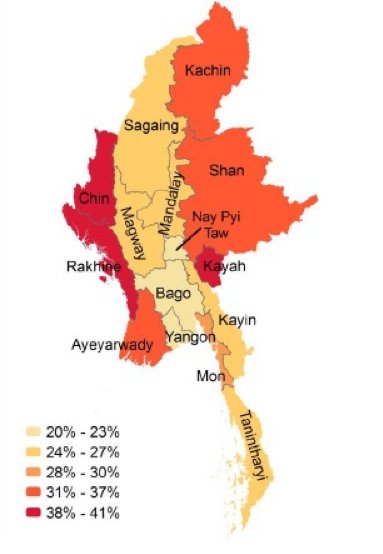
\includegraphics[width=0.5\linewidth]{figures/kayah1} 

}

\caption{Stunting prevalence by States and Regions}\label{fig:myanmarMap1}
\end{figure}

\begin{figure}[H]

{\centering 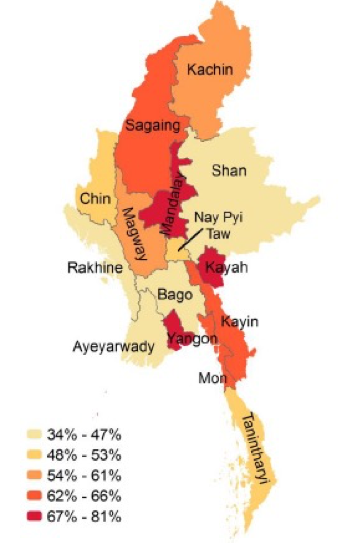
\includegraphics[width=0.5\linewidth]{figures/kayah2} 

}

\caption{Immunisation coverage by States and Regions}\label{fig:myanmarMap2}
\end{figure}

\begin{figure}[H]

{\centering 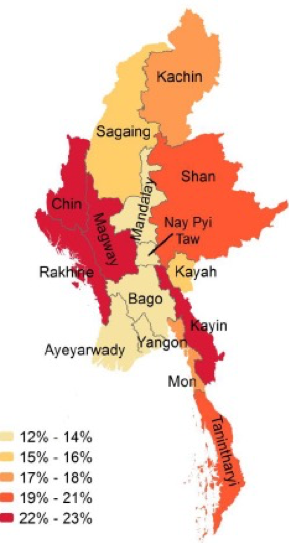
\includegraphics[width=0.5\linewidth]{figures/kayah3} 

}

\caption{Family planning unmet need by States and Regions}\label{fig:myanmarMap3}
\end{figure}

The NSPSP prioritizes the most geographically excluded and poorest States and Regions, and emphasizes the importance of including historically religious, ethnic, and other underserved minorities through increased cooperation and communication.

\hypertarget{objectives}{%
\section{Study aims and objectives}\label{objectives}}

To provide a basis for measuring and evaluating the outcomes and impact of the MCCT program over time, in line with the MSWRR's program to support maternal and child nutrition in support of the MS-NPAN by estimating current levels of indicators related to:

\begin{enumerate}
\def\labelenumi{\arabic{enumi}.}
\item
  Nutrition based on anthropometric measurements of child weight, height, and mid-upper arm circumference (MUAC) and maternal MUAC in Kayin State;
\item
  Behaviors related to nutrition, infant and young child feeding (IYCF), and health-seeking pratices among mothers in Kayin State; and,
\item
  Knowledge related to health, nutrition, and hygiene among pregnant women and mothers with under 5 children in Kayin state.
\end{enumerate}

\hypertarget{research-questions}{%
\subsection{Research Questions}\label{research-questions}}

\begin{enumerate}
\def\labelenumi{\arabic{enumi}.}
\item
  What are the current levels of indicators related to nutrition, infant and young child feeding (IYCF), and health-seeking behaviors of mothers and under 5 children in Kayin State?
\item
  What is the impact of the MCCT program on child stunting in Kayin State?
\item
  What is the impact of the MCCT program on maternal nutritional status in Kayin State?
\end{enumerate}

\hypertarget{methods}{%
\section{Methods}\label{methods}}

\hypertarget{design}{%
\subsection{Study design}\label{design}}

The study included two primary components:

\hypertarget{study1}{%
\subsubsection{Survey of selected households, villages, and townships}\label{study1}}

This was composed of three surveys.

\begin{enumerate}
\def\labelenumi{\arabic{enumi}.}
\item
  \textbf{Representative household survey} - The baseline survey was designed for the measurement and evaluation of outcomes over time by estimating the current levels of indicators related to nutrition, IYCF, and health-seeking behaviors. The baseline study was conducted during the roll-out of MCCT program in Kayin State.
\item
  \textbf{Village profiles} - Village level demographics, assets, and conditions were assessed in each of the selected villages in Kayin State.
\item
  \textbf{Township profiles} - Township profiles were developed from the township-level data collected from all townships in Kayin State from which sampled villages were from.
\end{enumerate}

This component of the study was designed to address research question 1 (Section \ref{research-questions}). The survey results were used to provide context to the results of the second study component (see Section \ref{study2}).

\hypertarget{sampling-frame}{%
\paragraph{Sampling frame}\label{sampling-frame}}

To assess the various outcome indicators for the assessment\footnote{Based on the earlier Chin assessment and based on feedback from various stakeholders.}, a two-stage cluster sample survey was implemented. The \textbf{first stage sample} was a sample of about 75 wards and villages tracts out of the total wards and villages tracts in Kayin State stratified into 1) \emph{urban}, 2) \emph{rural} and 3) \emph{hard-to-reach} areas. Stratification was based on administrative classifications and other characteristics such as remoteness and restricted access due to mixed administration. Sampling was proportional to population size of the ward or village tract. The \textbf{second stage sample}, also called the within-community sample, was a sample of households from the selected wards and villages tracts with mothers with children less than 5 years old. The second stage sample was selected using the list of household with children under 5 years of age from each village as identified by township General Administrative Department (GAD) whenever possible.

A total of about 14 households with pregnant mothers and mothers with children less than 5 years were sampled in each village. If a small community was selected that was likely to have fewer than the required number of eligible respondents, all eligible households and persons in that community are sampled by moving door-to-door. If a household had more than one mother with children under 5 years of age, all eligible women within the household were interviewed. In addition, all pregnant mothers present in the household of the respondents were measured for middle upper arm circumference (MUAC).

\hypertarget{sample-size-1}{%
\paragraph{Sample size estimation}\label{sample-size-1}}

Using childhood stunting as index indicator for sample size calculations, the sample size needed to detect a change of mean HAZ from 1.432 in Kayin State\footnote{Based on 2015 Myanmar Demographic and Health Survey \citep{MinistryofHealthandSports-MoHS/Myanmar2017}} to -0.932 with a calculated standard deviation 1.14406\footnote{Based on 2015 Myanmar Demographic and Health Survey \citep{MinistryofHealthandSports-MoHS/Myanmar2017}} was calculated. This is an equivalent drop in stunting prevalence of about 10\%. This equates to a sample size of 137 children less than 5 years old. Assuming a design effect for a cluster survey of 2, this sample size was inflated to 274. A sample size of 274 respondents was needed for each stratum (\emph{urban}, \emph{rural} and \emph{hard-to-reach}) in Kayin State giving a total of 822 respondents in total. Assuming a non-response rate of 20\% overall, a total of 330 respondents was the target sample for each stratum in Kayin State.

As described in the sampling frame above, a total of 25 villages per strata and 14 respondent mothers with children less than 5 years old were the target number of samples and a total of 350 respondents in each strata was the overall target in order to achieve at least 274. In Kayin state, a total of 1050 respondents was the overall target. This is anticipated to be more than enough sample size as per calculations above. For the selected respondents who were not present at the time of data collection, two revisits were conducted with the respondent classified as a non-responder after three unsuccessful attempts.

\hypertarget{study2}{%
\subsubsection{Quasi-experimental cohort study}\label{study2}}

As part of a longitudinal, quasi-experimental evaluation design, the baseline survey included a cohort of mothers and their children selected through specific study eligibility criteria based on eligibility and receipt of the services and benefits of the MCCT program. Once recruited, this cohort was assessed on appropriate indicators related to nutrition, IYCF and health-seeking behaviours at baseline. This same cohort will then be assessed at midline on the same set of appropriate and relevant indicators to detect any difference between those receiving benefits from the MCCT from those who are not based on a regression discontinuity analytical approach (see Section \ref{regression-discontinuity}).

This component of the study provides a statistically robust comparison between those exposed to the MCCT program and those who are not hence detecting the possible impact that the program has on a specific set of impact indicators.

Given the universal nature of the MCCT program and the need to create effective treatment and comparison groups to detect program impact, this study component used a similar regression discontinuity (RD) design as was developed and used for the MCCT evaluation in Chin State, but with distinct changes that address limitations of the latter \citep{MinistryofSocialWelfareReliefandResettlement2018}. This design was made possible by the fact that there is a specific cut-off point for program eligibility. Ultimately, the program (treatment) effect can be detected as a discontinuity in the regression line around this cut-off which in this case is a specific date that determines eligibility. The design is \emph{quasi-experimental}, since treatment and comparison groups were not selected at random but based on predefined characteristics.

\hypertarget{eligibility}{%
\paragraph{Eligibility criteria}\label{eligibility}}

Eligibility criteria depended on three factors:

\begin{itemize}
\item
  Date of start of recruitment into the MCCT program (1st October 2018)
\item
  Date of recruitment for study participants
\item
  Receipt of MCCT benefits
\end{itemize}

The optimal bandwidth of ages of the children to include in the study needed to be as close to the cut-off date as possible such that the ages of the children in the control and intervention groups will be roughly similarly distributed. This meant up to one month before and after the recruitment date of 1st October 2018. Given this, the following eligibility criteria were applied:

\textbf{Control group}

The criteria for eligibility to the control group of the study was women who gave birth on/after 1 September 2018 but before 1 October 2018 (i.e.~1 month before the MCCT registration cut-off).

\textbf{Intervention group}

The criteria for eligibility to the intervention group of the study was women who gave birth on or after 1 Oct 2018 but before 1 November 2018 (i.e.~1 month after the MCCT registration cut-off) and have been recruited into the MCCT program.

\hypertarget{sample-size-2}{%
\paragraph{Sample size and selection}\label{sample-size-2}}

The RD design effect was factored in for sample size calculations. This design effect was used to inflate standard randomized controlled trials (RCT) sample sizes in order to account for the RD design. The RD design effect was primarily influenced by the distribution of characteristics of the cut-off variable (i.e.~running variable) \citep{Bor2014}. Previous literature advises that if the running variable is normally distributed around the cut-off, then the design effect is approximately 2.75. If the running variable is uniformly distributed around the cut-off, the design effect is 4, and if it is bimodal in distribution, then the design effect can go up to 5 \citep{Schochet2009}.

Given that the running variable for this study is the start date of registration in relation to pregnancy, it was expected that there would be various peaks in number of pregnancies at specific time points following a general seasonal pattern not necessarily related to the cut-off date. The distribution is therefore likely multi-modal. So an assumption of at least 5 design effect for this RD design was taken into account.

Using prevalence of stunting as the index indicator for calculating sample size and using mean change in height-for-age z-score (HAZ) as the specific variable to use for assessing change, the same sample size calculation as in the survey was arrived at which was 137 for controls and 137 for intervention (total of 274).
However, given the very narrow bandwidth of inclusion into the study used (one month before and after the program start), it is likely that the universal population from which to select the cohort is quite small and that the total sample size of 274 is likely requiring an exhaustive sampling of all children born within the specified periods above. In this case, the inflation factor to account for design effect was not considered to be relevant given that an exhaustive sample will be drawn to begin with. Hence the 274 sample size for Kayin State was set as the target sample size.

\hypertarget{sample-recruitment}{%
\paragraph{Sample recruitment}\label{sample-recruitment}}

Sample recruitment utilised a full list or registry of births one month before and after the 1st of October 2018 in the wards and village tracts selected for the survey. As an exhaustive sample was needed, all fforts were undertaken to identify and recruit eligible women and their newborns into the study including engagement with the DSW in listing out and finding these births across Kayin state.

\hypertarget{data-collection}{%
\subsection{Data collection}\label{data-collection}}

Data was collected using an electronic data entry system based on the \textbf{Open Data Kit (ODK)} standard that runs on the Android operating software (OS) platform for mobile devices. The study instrument was encoded into the electronic data entry system platform and was served out of a secure aggregate server hosted by ONA\footnote{See \url{https://ona.io}}. Each data collector was provided with a tablet running on Android OS that was configured with the ODK application that receives the electronic data form. All measurements and answers by respondents were then recorded on the tablets and transmitted to the remote server whenever there was a mobile and/or wireless internet signal. This data collection system was not reliant on internet connection as the data collection could be performed offline, with the completed e-questionnaires saved on the interviewers' tablets. An internet connection was needed only when finalized encoded forms were ready to submit to the remote server, and this submission was done at regular intervals and timed when there was available internet connection for the data collectors. The survey teams aimed to submit forms on a daily basis.

\hypertarget{questionnaire-design}{%
\subsubsection{Questionnaire design:}\label{questionnaire-design}}

Structured questionnaires for the household survey, village profiles, and township profiles were developed in English and translated into Myanmar language. The household survey also included anthropometric measurements for weight, height and MUAC for all pregnant women, mothers, and every child up to five years of age in selected households. A separate form was developed for the anthropometric measurements.

The village profile questionnaire assessed various village level characteristics relevant to the study such as number of and distances to nearby markets, education, and health facilities; presence of community groups (e.g., Village Health Committees) and their functionality; presence of community volunteers (e.g., auxiliary midwives and community health workers); access and quality of water and sanitation facilities; and general agricultural practices.

The township profile questionnaire collected data on the township's population, geography, and governance, with summaries of key nutrition indicators.

Prior to the start of data collection, the household survey questionnaire was pilot tested to understand how well the wording and content, context effects, and interface design of the instruments performed in an actual survey setting and were revised as necessary. Respondents for field testing were purposively sampled from the same population as the baseline assessment (e.g., mothers from the study area, village leaders). Field testing was iterative with changes to the data collection instruments implemented immediately and the revised instrument was re-tested.

\hypertarget{training}{%
\subsection{Training of enumerators}\label{training}}

Different trainings were conducted based on the skill that was being trained and the type of personnel that was being trained.

\hypertarget{anthro-training}{%
\subsubsection{Anthropometric Training}\label{anthro-training}}

Recruited anthropometrists received an intensive 5-day training from an expert anthropometric measurement trainer with supervision by National Nutrition Center (NNC) and nutrition advisor(s). The training covered an introduction to the purpose of the study, nutritional indicators , anthropometry, accuracy and validity of measurements, utilization and equipment of the measurement tools (e.g., MUAC tape, weighing scales, measuring board), and electronic data entry. The training emphasized practice and standardization of the anthropometric measurements to be used during the study according to methods adapted from the \href{https://www.who.int/childgrowth/mgrs/en/}{WHO's Multicentre Growth Reference Study} \citep{DeOnis2004} and \href{https://intergrowth21.tghn.org}{INTERGROWTH-21 Project} \citep{Ismail2013} anthropometric training protocols.

During the training, women of reproductive age and children under five years of age were invited to participate as subjects, and each subject was measured twice by the expert trainer serving as gold standard and twice by each trainee. To assess inter- and intra-rater precision, the technical error of measurement (TEM) was calculated, with an acceptable TEM for an individual trainee defined as no more than twice that of the expert \citep{ulijaszek_kerr_1999}. Accuracy was assessed by calculating mean differences between the gold standard trainer and the trainee. Only participants who meet the required standard for accuracy and precision were selected for anthropometric data collection during the baseline assessment. The training was conducted in Myanmar language.

\hypertarget{interview-training}{%
\subsubsection{Interviewer and Supervisor Training}\label{interview-training}}

All supervisors and enumerators received an intensive 5-day training from study team members that covered the purposes of the study, informed consent procedures, the questionnaire guides and responses, electronic data entry, referral protocols for severe acute malnutrition, roles and responsibilities of all field staff, data quality assurance procedures, problem-solving, and conflict-sensitive approaches to data collection. The performance of trainees was assessed post-training during practice sessions.

\hypertarget{add-training}{%
\subsubsection{Additional Supervisor Training}\label{add-training}}

All supervisors received an additional 3 days of training from study team members that covered screening, random sampling method to identify respondents, quality control in the field, quality control of data entry and uploading, team management, and logistics.

\hypertarget{survy-management}{%
\subsection{Survey management and supervision}\label{survy-management}}

Five teams were responsible for data collection in Kayin State. During data collection, 1 field supervisor supervised 1 team each composed of 4 enumerators and 2 anthropometrists. Each team was expected to complete 14 household interviews and one village profile per day depending on feasibility. Community Partners International worked with the Central NNC and State/Region Nutrition Teams and nutrition experts in developing a referral guidelines and standard operating procedures to ensure that any women or children who were measured during the study and suspected of having severe acute malnutrition (SAM) were immediately referred to an appropriate health provider. Survey teams were provided with contact information of the nearest health providers to ensure timely referral. Alerts to refer women and children were programmed into the e-questionnaire on the ODK platform, based on WHO criteria for SAM.

\hypertarget{quality-control}{%
\subsection{Quality control}\label{quality-control}}

Quality control procedures throughout the assessment design, implementation, and analysis included:

\begin{itemize}
\item
  Translation, and pilot testing as described above;
\item
  Development of standard operating procedures and training manuals. CPI developed and distributed guidelines on data collection procedures, including the questionnaire and anthropometry methods, to all members of the data collection teams;
\item
  Training of data collectors where supervisors, enumerators, and anthropometrists practiced administering the questionnaire and checking and correcting questionnaires for accuracy and completeness. The performance of anthropometrists and data collectors were assessed in terms of confidence, independence, and reliability during practice sessions during the trainings, and based on results of an evaluation at the end of the training period;
\item
  Anthropometric devices were calibrated and supervisors re-assessed some of the anthropometric measurements at intervals. Maintenance and quality check of all the other devices were done regularly as per the manufacturer's instructions. Data collection was coordinated and continuously supervised by field supervisors and senior researchers.
\item
  The data collection tool was designed in such a way that any potential errors related to data entry were minimized by programmatically adding data entry checks that raise appropriate prompts to the data collector based on the potential error detected. The data collector was not allowed by the system to continue to the next field until the error has been corrected. For the anthropometric measurements, a test for the feasibility of the measurements taken based on the child's age and sex was implemented. If the measurement was above or below a certain threshold of feasible values, the system prompted the data collector to check their recording of the measurement, and to perform the measurement again. This approach was expected to pick up at least 90\% of possible errors due to data entry and measurement errors. to complement this, an algorithm was added to randomly ask the data collector to repeat the measurement, even if the result of the first measurement was plausible. This approach was expected to pick up at least 90\% of possible errors due to data entry and measurement errors.
\item
  The Data Manager reviewed the data in real-time as they were uploaded to the server. This was done using a purpose-built application called \texttt{myanmarMCCTchecks}\footnote{See \url{https://validmeasures.io/myanmarMCCTchecks}} that allows for routine data checks automatically. In most cases, the error was detected and corrected immediately due to the data quality assurance measures built into the ODK platform, but if necessary, the interviewer was requested to revisit the respondent. In this case, the corrected questionnaire was uploaded and the wrong one deleted, so that only correct, checked records were stored in the database.
\end{itemize}

\hypertarget{analysis}{%
\subsection{Data processing and analysis}\label{analysis}}

\hypertarget{processing-tools}{%
\subsubsection{Tools and methods}\label{processing-tools}}

Data handling, processing, analysis and reporting were done using \textbf{version 3.6.1} of the \href{https://cran.r-project.org}{R Language for Statistical Computing}\footnote{Can be downloaded from the \href{https://cran.r-project.org}{Comprehensive R Archive Network} where guidance on installing R is also available.} \citep{R2019}. The R package \textbf{myanmarMCCTdata} was developed to support the handling, processing and analysis of data collected for the study. The package includes functions to retrieve data from the \href{https://ona.io}{ONA} server database, to appropriately structure datasets, to check and clean data, to recode data to respective indicator sets, to estimate indicators and to perform appropriate comparative analysis specified by the analysis\footnote{See \url{https://validmeasures.org/myanmarMCCTdata} to learn more about the \textbf{myanmarMCCTdata} package and how data is handled and processed using this package.} \citep{myanmarData2019}. The package uses several other R packages that provide additional functions for data processing, analysis and reporting\footnote{For a full list of other R packages that \textbf{myanmarMCCTdata} depends on, see \url{https://validmeasures.org/myanmarMCCTdata}}.

The main motivation for using R was to achieve transparent and reproducible research between the study collaborators and with external reviewers and/or readers. Developing the \textbf{myanmarMCCTdata} R package is the first step towards this aim of transparency and reproducibility as any collaborator and/or reviewer can easily retrieve the same codebase for data handling, processing and analysis used by the primary researchers. The second step was writing reports (including this report) using R itself using a seamless integration between data analysis and reporting. This was achieved using R Markdown \citep{rmarkdown2018} for producting reports which included code chunks of how the data processed using \textbf{myanmarMCCTdata} functions were analysed to produce the results reported here. This report and the analysis herein, can be reviewed and reproduced by collaborators and reviewers by following instructions given \href{https://github.com/validmeasures/myanmarMCCTkayin}{here}.

\hypertarget{indicator-estimation}{%
\subsubsection{Indicator estimation}\label{indicator-estimation}}

Data was processed and recoded based on standard and established indicator definitions whenever available. For some indicators, modifications to standard definitions were made based on information requirements by stakekholders or study-specific definitions were established in order to achieve analysis requirements. Several recode functions were developed in R through the \textbf{myanmarMCCTdata} package for this purpose. The following indicator sets were assessed:

\hypertarget{mcct-program-coverage}{%
\paragraph{MCCT program coverage}\label{mcct-program-coverage}}

Given that actual exposure to the intervention is a key factor to assessing impact of the MCCT program, coverage was deemed important to assess and estimate. Based on eligibility criteria for MCCT, households were assessed whether they qualified for inclusion in MCCT. Households were also asked whether they were in the MCCT and receiving its benefits. These data were then used to assess program coverage defined as:

\[ \text{MCCT program coverage} ~ = ~ \frac{\text{Eligible households in MCCT program}}{\text{Total eligible households}} \]

This indicator was only estimated for the population survey sample component of the study.

\hypertarget{ppi}{%
\paragraph{Poverty probability index (PPI)}\label{ppi}}

The \href{https://www.povertyindex.org}{Poverty Probability Index (PPI)} is a poverty measurement tool that is statistically-sound, yet simple to use. The answers to 10 country-specific questions about a household's characteristics and asset ownership are scored to compute the likelihood that the household is living below a certain poverty line or definition\citep{InnovationsforPovertyAction2019}. PPI is used to identify households who are most likely to be poor or vulnerable to poverty.

The Myanmar MCCT survey collected answers to the 10 Myanmar-specific questions on household characteristics and asset ownership responses which were used to determine the household's PPI score based on the Myanmar national poverty line. The household's PPI score was then matched to poverty line/definition-specific lookup tables to determine the household's poverty probability. The matching of the PPI score to lookup tables was facilitated using the PPI lookup tables for Myanmar from the \texttt{ppitables} package \citep{Guevarra2019} for R.

\hypertarget{wash}{%
\paragraph{Water, sanitation and hygiene}\label{wash}}

Recoding for indicators for water, sanitation and hygiene (WASH) were based on standard indicator definitions provided by WHO and UNICEF \citep{WHOUNICEFJointMonitoringProgrammeforWaterSupplyandSanitation:2018vr, WorldHealthOrganization:2006vv}.

The following drinking water access indicators were assessed:

\begin{itemize}
\item
  Access to improved drinking water sources (regardless of collection time\footnote{Time to collect water from reported water source was not collected in baseline survey. The access to improved drinking water sources indicator does not take time into account. This indicator can be reframed as at least limited access to improved drinking water sources taking into account the definitions for limited and basic drinking water service.})
\item
  Access to unimproved drinking water sources only (unprotected dug well and unprotected spring)
\item
  Drinking water from surface water (directly from a river, dam, lake, pond, stream, canal/irrigation canal)
\item
  Probably safe drinking water based on appropriate water treatment method applied to water
\end{itemize}

These drinking water access indicators have been assessed for each of the three seasons (summer, rainy and winter season) experienced in Kayin and Kayin states.

In addition to drinking water access, the following drinking water use and storage behaviour was also assessed:

\begin{itemize}
\tightlist
\item
  Use of a water container/pot that is clean, covered and with a cup and handle
\end{itemize}

The following indicators on access to sanitation facilities were assessed:

\begin{itemize}
\item
  Access to improved sanitation facilities that are not shared with other households\footnote{This is termed as access to \textbf{basic} sanitation facilities as per current indicator definitions.}
\item
  Access to improved sanitation facilities that are shared with other households\footnote{This is termed as access to \textbf{limited} sanitation facilities as per current indicator definitions.}
\item
  Access to unimproved sanitation facilities
\item
  Use of open defecation
\end{itemize}

The following indicators on access to handwashing facilities were assessed:

\begin{itemize}
\item
  Access to handwashing facility on premises with soap and water\footnote{This is termed as access to \textbf{basic} handwashing facilities as per current indicator definitions.}
\item
  Access to handwashing facilities on premises without soap and water\footnote{This is termed as access to \textbf{limited} handwashing facilities as per current indicator definitions.}
\item
  No handwashing facilities
\end{itemize}

In addition, handwashing practices and behaviours were also assessed.

\hypertarget{fcs}{%
\paragraph{Food consumption score (FCS)}\label{fcs}}

The \textbf{Food Consumption Score (FCS)} is an index developed by the World Food program (WFP) in 1996 \citep{VulnerabilityAssessmentandMappingWorldFoodProgramme:2008ti}. The \textbf{FCS} is a household level indicator that aggregates food group diversity and frequency over the past 7 days. These food groups are then weighted according to their relative nutritional value. This means that food groups that are nutritionally-dense such as animal products are given greater weight than those containing less nutritionally dense foods such as tubers. The weights are then added up to come up with a household score which are then used to classify households into either poor, borderline, or acceptable food consumption. The \textbf{FCS} is a measure of quantity of caloric intake.

A brief questionnaire was used to ask respondents about the frequency of their households' consumption of eight different food groups over the previous seven days. The eight food groups are: main staples; pulses; vegetables; fruit; meat/fish; milk; sugar; and, oil. The frequency of consumption of these different food groups consumed by a household during the 7 days before the survey was then used to calculate a weighted diet diversity score for each household using the food group weights (Table \ref{tab:fcsWeights}) by multiplying the reported 7-day frequencies with the food group weights.

\newpage

\begin{longtable}[]{@{}cllr@{}}
\caption{\label{tab:fcsWeights} FCS food groups and weights}\tabularnewline
\toprule
\begin{minipage}[b]{0.07\columnwidth}\centering
\strut
\end{minipage} & \begin{minipage}[b]{0.47\columnwidth}\raggedright
\textbf{Food items}\strut
\end{minipage} & \begin{minipage}[b]{0.20\columnwidth}\raggedright
\textbf{Food groups}\strut
\end{minipage} & \begin{minipage}[b]{0.15\columnwidth}\raggedleft
\textbf{Weight}\strut
\end{minipage}\tabularnewline
\midrule
\endfirsthead
\toprule
\begin{minipage}[b]{0.07\columnwidth}\centering
\strut
\end{minipage} & \begin{minipage}[b]{0.47\columnwidth}\raggedright
\textbf{Food items}\strut
\end{minipage} & \begin{minipage}[b]{0.20\columnwidth}\raggedright
\textbf{Food groups}\strut
\end{minipage} & \begin{minipage}[b]{0.15\columnwidth}\raggedleft
\textbf{Weight}\strut
\end{minipage}\tabularnewline
\midrule
\endhead
\begin{minipage}[t]{0.07\columnwidth}\centering
1\strut
\end{minipage} & \begin{minipage}[t]{0.47\columnwidth}\raggedright
Maize , maize porridge, rice, sorghum,
millet pasta, bread and other cereals
Cassava, potatoes and sweet potatoes,
other tubers, plantains\strut
\end{minipage} & \begin{minipage}[t]{0.20\columnwidth}\raggedright
Main staples\strut
\end{minipage} & \begin{minipage}[t]{0.15\columnwidth}\raggedleft
2\strut
\end{minipage}\tabularnewline
\begin{minipage}[t]{0.07\columnwidth}\centering
2\strut
\end{minipage} & \begin{minipage}[t]{0.47\columnwidth}\raggedright
Beans, peas, groundnuts and cashew nuts\strut
\end{minipage} & \begin{minipage}[t]{0.20\columnwidth}\raggedright
Pulses\strut
\end{minipage} & \begin{minipage}[t]{0.15\columnwidth}\raggedleft
3\strut
\end{minipage}\tabularnewline
\begin{minipage}[t]{0.07\columnwidth}\centering
3\strut
\end{minipage} & \begin{minipage}[t]{0.47\columnwidth}\raggedright
Vegetables, leaves\strut
\end{minipage} & \begin{minipage}[t]{0.20\columnwidth}\raggedright
Vegetables\strut
\end{minipage} & \begin{minipage}[t]{0.15\columnwidth}\raggedleft
1\strut
\end{minipage}\tabularnewline
\begin{minipage}[t]{0.07\columnwidth}\centering
4\strut
\end{minipage} & \begin{minipage}[t]{0.47\columnwidth}\raggedright
Fruits\strut
\end{minipage} & \begin{minipage}[t]{0.20\columnwidth}\raggedright
Fruits\strut
\end{minipage} & \begin{minipage}[t]{0.15\columnwidth}\raggedleft
1\strut
\end{minipage}\tabularnewline
\begin{minipage}[t]{0.07\columnwidth}\centering
5\strut
\end{minipage} & \begin{minipage}[t]{0.47\columnwidth}\raggedright
Beef, goat, poultry, pork, eggs and
fish\strut
\end{minipage} & \begin{minipage}[t]{0.20\columnwidth}\raggedright
Meat and fish\strut
\end{minipage} & \begin{minipage}[t]{0.15\columnwidth}\raggedleft
4\strut
\end{minipage}\tabularnewline
\begin{minipage}[t]{0.07\columnwidth}\centering
6\strut
\end{minipage} & \begin{minipage}[t]{0.47\columnwidth}\raggedright
Milk yoghurt and other diary\strut
\end{minipage} & \begin{minipage}[t]{0.20\columnwidth}\raggedright
Milk\strut
\end{minipage} & \begin{minipage}[t]{0.15\columnwidth}\raggedleft
4\strut
\end{minipage}\tabularnewline
\begin{minipage}[t]{0.07\columnwidth}\centering
7\strut
\end{minipage} & \begin{minipage}[t]{0.47\columnwidth}\raggedright
Sugar and sugar products, honey\strut
\end{minipage} & \begin{minipage}[t]{0.20\columnwidth}\raggedright
Sugar\strut
\end{minipage} & \begin{minipage}[t]{0.15\columnwidth}\raggedleft
0.5\strut
\end{minipage}\tabularnewline
\begin{minipage}[t]{0.07\columnwidth}\centering
8\strut
\end{minipage} & \begin{minipage}[t]{0.47\columnwidth}\raggedright
Oils, fats and butter\strut
\end{minipage} & \begin{minipage}[t]{0.20\columnwidth}\raggedright
Oil\strut
\end{minipage} & \begin{minipage}[t]{0.15\columnwidth}\raggedleft
0.5\strut
\end{minipage}\tabularnewline
\begin{minipage}[t]{0.07\columnwidth}\centering
9\strut
\end{minipage} & \begin{minipage}[t]{0.47\columnwidth}\raggedright
Spices, tea, coffee, salt, fish powder,
small amounts of milk for tea.\strut
\end{minipage} & \begin{minipage}[t]{0.20\columnwidth}\raggedright
Condiments\strut
\end{minipage} & \begin{minipage}[t]{0.15\columnwidth}\raggedleft
0\strut
\end{minipage}\tabularnewline
\bottomrule
\end{longtable}

All the weighted consumption frequencies were then summed up per household to arrive at the FCS for the specific household. Then, Using the appropriate thresholds (Table \ref{tab:fcsThresholds}), each household is classified accordingly based on their FCS.

\begin{longtable}[]{@{}ll@{}}
\caption{\label{tab:fcsThresholds} FCS classification thresholds}\tabularnewline
\toprule
\begin{minipage}[b]{0.16\columnwidth}\raggedright
\textbf{FCS}\strut
\end{minipage} & \begin{minipage}[b]{0.20\columnwidth}\raggedright
\textbf{Profiles}\strut
\end{minipage}\tabularnewline
\midrule
\endfirsthead
\toprule
\begin{minipage}[b]{0.16\columnwidth}\raggedright
\textbf{FCS}\strut
\end{minipage} & \begin{minipage}[b]{0.20\columnwidth}\raggedright
\textbf{Profiles}\strut
\end{minipage}\tabularnewline
\midrule
\endhead
\begin{minipage}[t]{0.16\columnwidth}\raggedright
0 - 21\strut
\end{minipage} & \begin{minipage}[t]{0.20\columnwidth}\raggedright
Poor\strut
\end{minipage}\tabularnewline
\begin{minipage}[t]{0.16\columnwidth}\raggedright
21.5 - 35\strut
\end{minipage} & \begin{minipage}[t]{0.20\columnwidth}\raggedright
Borderline\strut
\end{minipage}\tabularnewline
\begin{minipage}[t]{0.16\columnwidth}\raggedright
\(>\) 35\strut
\end{minipage} & \begin{minipage}[t]{0.20\columnwidth}\raggedright
Acceptable\strut
\end{minipage}\tabularnewline
\bottomrule
\end{longtable}

\hypertarget{fcsn}{%
\paragraph{Food consumption score nutrition quality}\label{fcsn}}

In addition to the standard FCS, WFP has devices a set of nutritional adequacy indicators that assess the nutrition quality of the household diet using the data provided by a slightly modified FCS questionnaire that disaggregates some of the food groups into sub-food groups known to contain vitamin A, protein and heme-iron. This is called the Food Consumption Score Nutrition Quality Analysis or FCS-N \citep{WorldFoodProgramme:2015tn}. The FCS-N focuses on three nutrients - vitamin A, iron and protein - to assess the nutrition adequacy of a household's diet. The FCS-N was calculated by first aggregating the individual food groups into nutrient-rich food groups shown in Table \ref{tab:fcs3}.

\begin{table}[H]

\caption{\label{tab:fcs3}Food groups classified by nutrients-of-interest for FCS-N}
\centering
\begin{tabular}[t]{l>{\raggedright\arraybackslash}p{8cm}}
\toprule
\textbf{Nutrients} & \textbf{Food Groups}\\
\midrule
\rowcolor{gray!6}  Vitamin A-rich foods & Dairy, organ meat, eggs, orange vegetables, green leafy vegetables and orange fruits\\
Protein-rich foods & Pulses, dairy, flesh meat, organ meat, fish and eggs\\
\rowcolor{gray!6}  Heme iron-rich foods & Flesh meat, organ meat, fish\\
\bottomrule
\end{tabular}
\end{table}

Households were then classified by their frequency of consumption of the three nutrients of interest.

\begin{table}[H]

\caption{\label{tab:fcs4}FCS-N categories based on nutrient-rich food groups consumption}
\centering
\begin{tabular}[t]{lr}
\toprule
\textbf{Category} & \textbf{No. of days of consumption}\\
\midrule
\rowcolor{gray!6}  Never & 0 days\\
Sometimes & 1-6 days\\
\rowcolor{gray!6}  At least daily & 7 or more days\\
\bottomrule
\end{tabular}
\end{table}

\hypertarget{csi}{%
\paragraph{Coping strategy index}\label{csi}}

The coping strategy index or CSI is a simple indicator that reveals how households manage or cope with shortfalls in food consumption. It is based on a list of possible behaviours that households may use as strategies for coping with conditions of having little or no food to eat \citep{Maxwell:2008vh}. The CSI combines the frequency by which a behaviour is utilised and the severity of each strategy used. There are two variations of the CSI. One assesses food consumption behaviours or strategies employed by the household in response to food insecurity (consumption-based CSI) while the other looks into the longer term, livelihoods-based strategies employed by households (livelihoods-based CSI).

The consumption-based coping strategy index (CCSI) used in this study was based on the reduced CSI questionnaire in order to allow for comparability between results for states and over time. The reduced CSI is based on 5 behaviours and corresponding severity weights for each as shown below.

\begin{table}[H]

\caption{\label{tab:csi1}Reduced CSI strategies/behaviours and their corresponding severity weights}
\centering
\begin{tabular}[t]{lr}
\toprule
\textbf{Behaviours/Strategies} & \textbf{Severity Weights}\\
\midrule
\rowcolor{gray!6}  Rely on less preferred and less expensive food & 1\\
Borrow food or rely on help from a relative or friend & 2\\
\rowcolor{gray!6}  Limit portion size at mealtimes & 1\\
Restrict consumption by adults in order for small children to eat & 3\\
\rowcolor{gray!6}  Reduce number of meals eaten in a day & 1\\
\bottomrule
\end{tabular}
\end{table}

The CCSI was calculated by multiplying the reported frequency of utilising a coping behaviour by the corresponding severity weight shown in Table \ref{tab:csi1} and then taking the aggregate of these weighted scores. The CCSI is a continuous variable and the mean CCSI is used to describe the level of utilisation of coping strategies by households.

The livelihoods based coping strategies index or LCSI was used to better understand a household's longer term coping capacity to food insecurity. The respondent was asked to recall whether in the past 30 days their household has engaged in any of a set of 10 coping behaviours/strategies due to a lack of food or lack of money to buy food. These behaviours/categories were categorised into \emph{stress} strategies, \emph{crisis} strategies and \emph{emergency} strategies. Based on the respondent's responses, their household was classified into the most severe strategy reported.

\hypertarget{hfes}{%
\paragraph{Household food expenditure share}\label{hfes}}

Taking household expenditure as a proxy of income, the proportion of this expenditure spent on food is an indicator of household food security. A household that is more food insecure spends a bigger proportion of income on food. This indicator was calculated from the various monetary values of household spending grouped into food and non-food items. The share of household expenditure on food was estimated as follows:

\[ \text{Household food expenditure share} ~ = ~ \frac{\sum{\text{Household expenditure on food}}}{\sum{\text{Total household expenditure}}} ~ \times ~ 100 \]

~

The following (see Table \ref{tab:hfes1}) commonly used thresholds for classifying household food insecurity based on its food expenditure share were used:

\begin{table}[H]

\caption{\label{tab:hfes1}Commonly used HFES thresholds}
\centering
\begin{tabular}[t]{ll}
\toprule
HFES & Food insecurity classification\\
\midrule
\rowcolor{gray!6}  > 75\% & Very vulnerable\\
65-75\% & High food insecurity\\
\rowcolor{gray!6}  50-65\% & Medium food insecurity\\
< 50\% & Low food insecurity\\
\bottomrule
\end{tabular}
\end{table}

\hypertarget{chealth}{%
\paragraph{Child health}\label{chealth}}

The child health indicators of the Myanmar MCCT program Evaluation include the following:

\begin{itemize}
\item
  Immunisation coverage;
\item
  Period prevalence of childhood illnesses;
\item
  Treatment-seeking behaviour for childhood illnesses; and,
\item
  Prevalence of low birthweight
\end{itemize}

\newpage

\textbf{Immunisation coverage}

Coverage of the expanded program on immunisation (EPI) in Myanmar was based on the 2016 revised routine vaccination schedule when the pneumococcal and inactivated polio vaccine injection were introduced \citep{MoHMyanmar:2016wp} (see Table \ref{tab:epi1}).

\begin{table}[H]

\caption{\label{tab:epi1}Myanmar EPI Schedule 2016}
\centering
\begin{tabular}[t]{ll}
\toprule
\textbf{Dose/Age} & \textbf{Vaccine}\\
\midrule
 & BCG\\
\cmidrule{2-2}
\multirow{-2}{*}{\raggedright\arraybackslash At birth} & Hepatitis B\\
\cmidrule{1-2}
 & BCG\\
\cmidrule{2-2}
 & DPT, Hepatitis B, HiB\\
\cmidrule{2-2}
 & Pentavalent 1\\
\cmidrule{2-2}
 & Pneumococcal Conjugate Vaccine 1\\
\cmidrule{2-2}
\multirow{-5}{*}{\raggedright\arraybackslash First Dose (2nd month)} & Oral Polio Vaccine 1\\
\cmidrule{1-2}
 & DPT, Hepatitis B, HiB\\
\cmidrule{2-2}
 & Pentavalent 2\\
\cmidrule{2-2}
 & Pneumococcal Conjugate Vaccine 2\\
\cmidrule{2-2}
 & Oral Polio Vaccine 2\\
\cmidrule{2-2}
\multirow{-5}{*}{\raggedright\arraybackslash Second dose (4th month)} & Inactivated Polio Vaccine\\
\cmidrule{1-2}
 & DPT, Hepatitis, HiB\\
\cmidrule{2-2}
 & Pentavalent 3\\
\cmidrule{2-2}
 & Pneumococcal Conjugate Vaccine 3\\
\cmidrule{2-2}
\multirow{-4}{*}{\raggedright\arraybackslash Third dose (6th month)} & Oral Polio Vaccine 3\\
\cmidrule{1-2}
Fourth dose (9th month) & Measles - Rubella\\
\cmidrule{1-2}
Fifth dose (18th Month) & Measles\\
\bottomrule
\end{tabular}
\end{table}

Immunisation coverage indicators were calculated according to standard indicator definitions for children 12-23 months old \citep{WorldHealthOrganization:2005vp, WorldHealthOrganization:1991uh, HoshawWoodard:2001vm}.

In addition to the standard indicators, age-appropriate immunisation coverage indicators were calculated based on Myanmar's EPI schedule. This was done to be able to maximise the full sample size of children 0-59 months old and to assess whether children at various ages receive the appropriate vaccination as per Myanmar EPI schedule. This is similar to approaches used by other researchers to assess age-appropriate immunisation coverage \citep[\citet{Dombkowski:2004bt}]{Kidane:2004uy, Tadesse:2009dm, Odutola:2015bm}

\newpage

\textbf{Period prevalence of childhood illnesses and treatment-seeking}

Mothers' report of their children's illness specifically diarrhoea, fever\footnote{Fever is used as a proxy for illnesses due to an infection such as malaria} or cough\footnote{Cough is used as a proxy for an acute respiratory infection (ARI)}, in the past 2 weeks provided the data for assessing the period prevalence of these childhood illnesses. Then, for those whose children had been ill, mothers' reported on whether treatment was sought, where it was sought and whether payment for treatment was required was used to assess treatment-seeking.

\textbf{Child birthweight}

Child birthweight was assessed based on either mother's report of their child's birthweight or by recorded birthweight on the child's health card. However, for purposes of accuracy, only the recorded birthweight on a health card was used to determine whether a child was born with low birth weight. Children with birthweight of less than 2500 grams were classified as being born with low birthweight \citep{Woertman:1993hp, Kelly:1997wa}.

\hypertarget{cnut}{%
\paragraph{Child nutrition}\label{cnut}}

The Myanmar MCCT program evaluation assessed the following child nutrition indicators:

\textbf{Childhood undernutrition}

Respective childhood undernutrition indices for childhood stunting, childhood wasting and childhood underweight were assessed. The height-for-age z-scores (HAZ), weight-for-height z-scores (WAZ) and weight-for-age z-scores of each 6-59 month old child in the sample were calculated using the R package \textbf{zscorer}\footnote{See \url{https://nutriverse.io/zscorer} for details on how the z-scores are calculated} \citep{zscorer2019}. Once z-score values were calculated, implausible z-score values were flagged using the WHO Growth Standards flagging criteria \citep{WorldHealthOrganizationWHO2006}. This was facilitated through the \textbf{nutricheckr} R package\footnote{See \url{https://nutriverse.io/nutricheckr} for details on how the flagging criteria is applied} \citep{nutricheckr2019}. Further anthropometric data quality checks were performed using \textbf{nipnTK}\footnote{See \url{https://nutriverse.io/nipnTK} for details on how anthropometric data quality check is performed using the \textbf{nipnTK} R package} \citep{nipnTK2019} R package which is based on an anthropometric data quality check toolkit developed and produced by the \href{http://www.nipn-nutrition-platforms.org}{National Information Platforms for Nutrition (NIPN)} and funded by the European Union.

\textbf{Infant and young child feeding}

Infant and young child feeding indicators were assessed based on standard WHO and UNICEF definitions \citep{WorldHealthOrganization:2008vw}. The following indicators were assessed:

\begin{itemize}
\item
  Exclusive breastfeeding
\item
  Early initiation of breastfeeding
\item
  Minimum meal frequency
\item
  Minimum dietary diversity
\item
  Minimum acceptable diet
\end{itemize}

\hypertarget{mhealth}{%
\paragraph{Maternal health}\label{mhealth}}

A standard set of maternal health indicators covering \emph{family planning}, \emph{antenatal care}, \emph{birth/delivery}, \emph{postnatal care} and \emph{newborn care} were assessed.

\hypertarget{mnut}{%
\paragraph{Maternal nutrition}\label{mnut}}

The following maternal nutrition indicators were assessed:

\textbf{Maternal undernutrition}

Maternal undernutrition was assessed based on MUAC. No consensus on MUAC cut-offs to determine maternal acute undernutrition have been identified and currently used cut-offs are specifically for pregnant and lactating women (PLW). Current research suggest that a cut-off of 23 cms is the most appropriate for PLW \citep{Ververs:2013ee} instead of the commonly used 18.5 and 21 cms cutoffs in supplementation programmes for PLW. Given that the Myanmar MCCT dataset has data for women of reproductive age and not only PLW, the 18.5 and 21 cms cutoffs were used to assess levels of acute undernutrition in mothers (see Table \ref{tab:manthro1}).

\begin{table}[H]

\caption{\label{tab:manthro1}MUAC cut-offs for maternal acute undernutrition}
\centering
\begin{tabular}[t]{ll}
\toprule
\textbf{MUAC cut-offs} & \textbf{Classification}\\
\midrule
\rowcolor{gray!6}  < 21 & Global acute undernutrition\\
18.5 to 21 & Moderate acute undernutrition\\
\rowcolor{gray!6}  < 18.5 & Severe acute undernutrition\\
\bottomrule
\end{tabular}
\end{table}

\textbf{Minimum dietary diversity for women}

Minimum dietary diversity for women or MDD-W is a dichotomous indicator of whether or not women 15--49 years of age have consumed at least five out of ten defined food groups the previous day or night. The proportion of women 15--49 years of age who reach this minimum in a population can be used as a proxy indicator for higher micronutrient adequacy, one important dimension of diet quality.

The indicator is calculated as follows:

\[ \text{MDD-W} = \frac{\text{Women 15-49 years of age who consumed 5 out of 10 food groups in the previous day or night}}{\text{Women 15-49 years of age}} \]

The ten food groups are:

\begin{enumerate}
\def\labelenumi{\arabic{enumi}.}
\tightlist
\item
  Grains, white roots and tubers, and plantains
\item
  Pulses (beans, peas and lentils)
\item
  Nuts and seeds
\item
  Dairy
\item
  Meat, poultry and fish
\item
  Eggs
\item
  Dark green leafy vegetables
\item
  Other vitamin A-rich fruits and vegetables
\item
  Other vegetables
\item
  Other fruits
\end{enumerate}

A fully reproducible data processing report can be reviewed \href{https://github.com/validmeasures/myanmarMCCTprocessing}{here}.

Using the recoded data for indicators, population-level estimates with 95\% confidence limits of these indicators were calculated using standard classical estimation techniques. Proportion-type indicators were estimated by getting the proportion of those having the indicator of interest out of the total sample. The 95\% confidence limits for a proportion-type indicator was estimated using the following formula:

\[
\begin{aligned}
\text{95\% confidence limits} & ~ = ~ p ~ \pm ~ 1.96 ~ \times ~ \sqrt{\frac{p ~ \times ~ (1 ~ - ~ p)}{n ^ 2}} \\
\\
where: & \\
\\
p & ~ = ~ \text{proportion estimate} \\
n & ~ = ~ \text{sample size}
\end{aligned}
\]

Indicators requiring the calculation of the population mean were estimated by calculating the mean of the sample for the indicator of interest. The 95\% confidence limits for a population mean indicator was estimated using the following formula:

\[
\begin{aligned}
\text{95\% confidence limits} & ~ = ~ \sigma ~ \pm ~ 1.96 ~ \times ~ \frac{SD}{\sqrt{n}} \\
\\
where: & \\
\\
\sigma & ~ = ~ \text{sample mean} \\
SD & ~ = ~ \text{standard deviation} \\
n & ~ = ~ \text{sample size}
\end{aligned}
\]

Indicator estimation was performed on the dataset for respondents for the population-based survey component of the study.

\hypertarget{regression-discontinuity}{%
\subsubsection{Regression discontinuity}\label{regression-discontinuity}}

Using data from respondents who quality for eligibility to the second component of the study, outcome nutrition indicators for children and mothers were plotted by date of birth of the index child to demonstrate whether a regression discontinuity on the indicators of interest were demonstrable between those who are not benefitting from the MCCT program (on the basis of being born up to a month before the start of the program) and those who are (born up to a month after start of the program). Discontinuity was detected visually through the plot and statistically by testing any difference between the regression line of those in the control group to the regression line of those in the treatment group.

\hypertarget{results}{%
\section{Results}\label{results}}

\hypertarget{study1-results}{%
\subsection{Population-representative survey}\label{study1-results}}

\hypertarget{mcct-coverage}{%
\subsubsection{MCCT program coverage}\label{mcct-coverage}}

MCCT program coverage is extremely low for a program that is meant to universally cover children less than 24 months old. In urban areas, only 30\% of eligible households are enrolled in MCCT. This proportion drops to a little over half in rural areas and in hard-to-reach areas. More eligible wealthier households are covered by the program compared to eligible poorer households. On average, eligible households received about 2 cash transfers to date.

\begin{table}[H]

\caption{\label{tab:mcct1table}MCCT program coverage}
\centering
\fontsize{10}{12}\selectfont
\begin{tabular}[t]{>{\bfseries}l>{\bfseries}l>{\ttfamily}r>{\ttfamily}r}
\toprule
 &  & \makecell[c]{In MCCT\\(\%)} & \makecell[c]{Number\\of\\cash\\transfers\\received}\\
\midrule
\addlinespace[0.3em]
\multicolumn{4}{l}{\textbf{Kayin}}\\
\addlinespace[0.3em]
\multicolumn{4}{l}{\textit{\textbf{Geographic}}}\\
\hspace{1em}\hspace{1em} & Rural & 16.2 & 1.7\\
\cmidrule{2-4}
\hspace{1em}\hspace{1em} & Urban & 29.4 & 2.5\\
\cmidrule{2-4}
\hspace{1em}\hspace{1em} & Hard-to-reach & 13.6 & 1.8\\
\cmidrule{2-4}
\addlinespace[0.3em]
\multicolumn{4}{l}{\textit{\textbf{Wealth}}}\\
\hspace{1em}\hspace{1em} & Wealthiest & 26.4 & 2.5\\
\cmidrule{2-4}
\hspace{1em}\hspace{1em} & Wealthy & 26.2 & 2.2\\
\cmidrule{2-4}
\hspace{1em}\hspace{1em} & Medium & 16.5 & 1.9\\
\cmidrule{2-4}
\hspace{1em}\hspace{1em} & Poor & 7.5 & 1.8\\
\cmidrule{2-4}
\hspace{1em}\hspace{1em} & Poorest & 15.0 & 1.4\\
\bottomrule
\end{tabular}
\end{table}

MCCT is received mostly through the village head. For hard-to-reach areas and for poor households, the EHO also served as means of disbursements of MCCT (see Table \ref{tab:mcct2table}). MCCT is used predominanlty for food and clothes and the mother is the usual decisionmaker for how to use the cash transfer (see Table \ref{tab:mcct3table}).

\begin{table}[H]

\caption{\label{tab:mcct2table}How MCCT is received}
\centering
\fontsize{10}{12}\selectfont
\begin{tabular}[t]{>{\bfseries}l>{\bfseries}l>{\ttfamily}r>{\ttfamily}r>{\ttfamily}r>{\ttfamily}r>{\ttfamily}r>{\ttfamily}r>{\ttfamily}r}
\toprule
 &  & \makecell[c]{Mobile\\programme\\(\%)} & \makecell[c]{Wave\\money\\(\%)} & \makecell[c]{Village\\head/\\GAD\\(\%)} & \makecell[c]{EHO\\(\%)} & \makecell[c]{CBO\\(\%)} & \makecell[c]{Midwife\\(\%)} & \makecell[c]{Health\\staff\\(\%)}\\
\midrule
\addlinespace[0.3em]
\multicolumn{9}{l}{\textbf{Kayin}}\\
\addlinespace[0.3em]
\multicolumn{9}{l}{\textit{\textbf{Geographic}}}\\
\hspace{1em}\hspace{1em} & Rural & 0 & 0 & 84.9 & 3.8 & 0.0 & 11.3 & 0.0\\
\cmidrule{2-9}
\hspace{1em}\hspace{1em} & Urban & 0 & 0 & 94.8 & 0.0 & 0.0 & 0.0 & 0.0\\
\cmidrule{2-9}
\hspace{1em}\hspace{1em} & Hard-to-reach & 0 & 0 & 37.8 & 23.2 & 1.2 & 17.1 & 11.0\\
\cmidrule{2-9}
\addlinespace[0.3em]
\multicolumn{9}{l}{\textit{\textbf{Wealth}}}\\
\hspace{1em}\hspace{1em} & Wealthiest & 0 & 0 & 89.5 & 0.0 & 0.0 & 9.2 & 1.3\\
\cmidrule{2-9}
\hspace{1em}\hspace{1em} & Wealthy & 0 & 0 & 72.7 & 7.6 & 1.5 & 4.5 & 4.5\\
\cmidrule{2-9}
\hspace{1em}\hspace{1em} & Medium & 0 & 0 & 66.7 & 11.1 & 0.0 & 3.7 & 3.7\\
\cmidrule{2-9}
\hspace{1em}\hspace{1em} & Poor & 0 & 0 & 64.3 & 35.7 & 0.0 & 0.0 & 0.0\\
\cmidrule{2-9}
\hspace{1em}\hspace{1em} & Poorest & 0 & 0 & 56.8 & 13.5 & 0.0 & 21.6 & 8.1\\
\bottomrule
\end{tabular}
\end{table}

\begin{table}[H]

\caption{\label{tab:mcct3table}How MCCT is used and who decides}
\centering
\fontsize{10}{12}\selectfont
\begin{tabular}[t]{>{\bfseries}l>{\bfseries}l>{\ttfamily}r>{\ttfamily}r>{\ttfamily}r>{\ttfamily}r>{\ttfamily}r>{\ttfamily}r>{\ttfamily}r}
\toprule
\multicolumn{2}{c}{ } & \multicolumn{4}{c}{MCCT used for...} & \multicolumn{3}{c}{Decided by...} \\
\cmidrule(l{3pt}r{3pt}){3-6} \cmidrule(l{3pt}r{3pt}){7-9}
 &  & \makecell[c]{Food\\(\%)} & \makecell[c]{Education\\(\%)} & \makecell[c]{Housing\\(\%)} & \makecell[c]{Clothes\\(\%)} & \makecell[c]{Self\\(\%)} & \makecell[c]{Husband\\(\%)} & \makecell[c]{Other\\household\\head\\(\%)}\\
\midrule
\addlinespace[0.3em]
\multicolumn{9}{l}{\textbf{Kayin}}\\
\addlinespace[0.3em]
\multicolumn{9}{l}{\textit{\textbf{Geographic}}}\\
\hspace{1em}\hspace{1em} & Rural & 45.2 & 0 & 3.2 & 45.2 & 89.7 & 5.2 & 0.0\\
\cmidrule{2-9}
\hspace{1em}\hspace{1em} & Urban & 68.2 & 0 & 2.3 & 15.9 & 95.4 & 2.8 & 1.8\\
\cmidrule{2-9}
\hspace{1em}\hspace{1em} & Hard-to-reach & 85.7 & 0 & 0.0 & 4.8 & 86.8 & 13.2 & 0.0\\
\cmidrule{2-9}
\addlinespace[0.3em]
\multicolumn{9}{l}{\textit{\textbf{Wealth}}}\\
\hspace{1em}\hspace{1em} & Wealthiest & 43.8 & 0 & 3.1 & 28.1 & 92.5 & 7.5 & 0.0\\
\cmidrule{2-9}
\hspace{1em}\hspace{1em} & Wealthy & 87.5 & 0 & 0.0 & 12.5 & 91.2 & 5.9 & 2.9\\
\cmidrule{2-9}
\hspace{1em}\hspace{1em} & Medium & 57.1 & 0 & 4.8 & 28.6 & 90.4 & 3.8 & 0.0\\
\cmidrule{2-9}
\hspace{1em}\hspace{1em} & Poor & 100.0 & 0 & 0.0 & 0.0 & 94.1 & 5.9 & 0.0\\
\cmidrule{2-9}
\hspace{1em}\hspace{1em} & Poorest & 71.4 & 0 & 0.0 & 28.6 & 88.9 & 11.1 & 0.0\\
\bottomrule
\end{tabular}
\end{table}

\hypertarget{ppi-results}{%
\subsubsection{Poverty probability index}\label{ppi-results}}

\begin{figure}[H]

{\centering 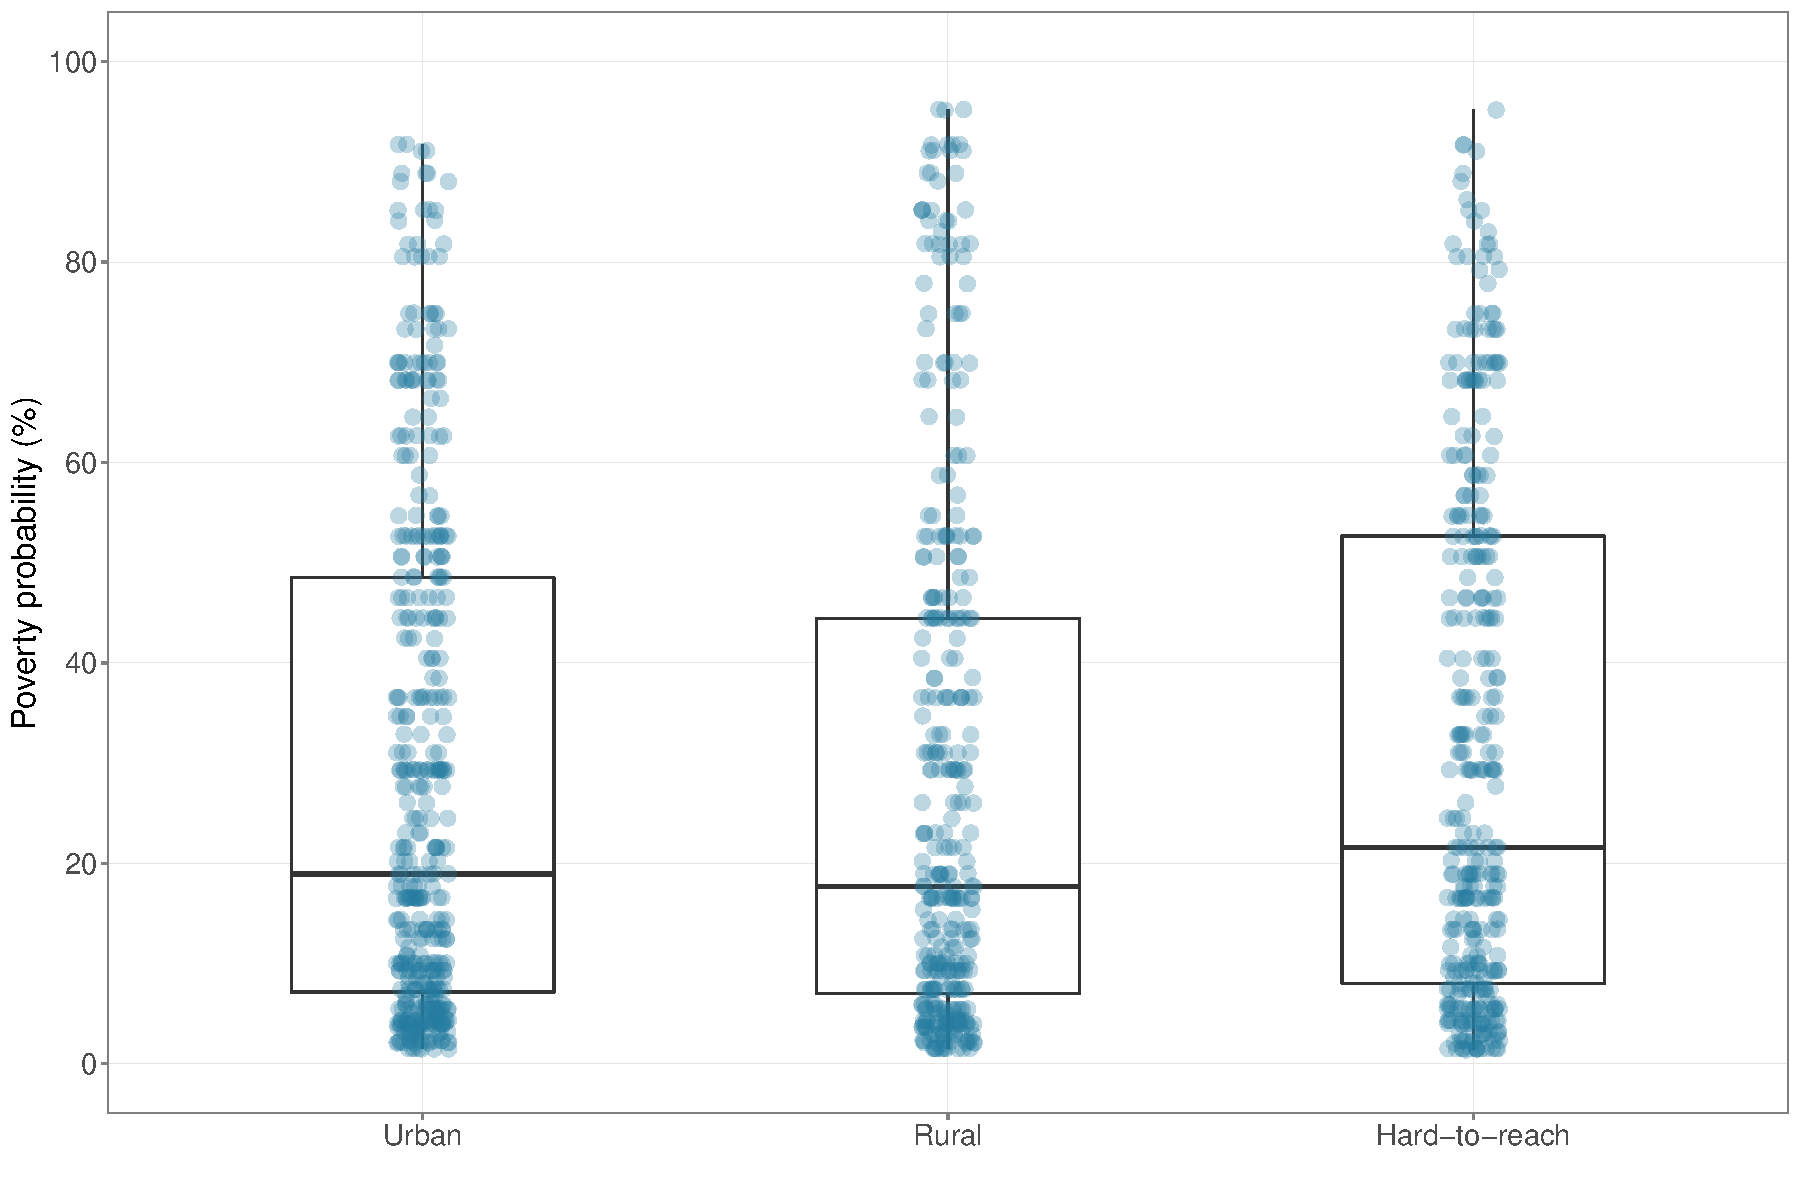
\includegraphics{kayinReport_files/figure-latex/ppiTable-1} 

}

\caption{Poverty probability index by location type}\label{fig:ppiTable}
\end{figure}

Poverty probability of households across different locations in Kayin state show high variability ranging from as low as 1.4\% to as high as a little over 95\%. This distribution of poverty is roughly similar across urban, rural and hard-to-reach areas as seen in Figure \ref{fig:ppiTable} above.

The poverty probabilities were primarily used to classify households into wealth quintiles which was subsequently used for wealth stratification of indicator results.

\hypertarget{fcs-results}{%
\subsubsection{Food consumption score}\label{fcs-results}}

\begin{table}[H]

\caption{\label{tab:fcs1table}Food consumption score}
\centering
\fontsize{12}{14}\selectfont
\begin{tabular}[t]{>{\bfseries}l>{\bfseries}l>{\ttfamily}r>{\ttfamily}r>{\ttfamily}r>{\ttfamily}r}
\toprule
 &  & \makecell[c]{Mean\\food\\consumption\\score} & \makecell[c]{Poor\\(\%)} & \makecell[c]{Borderline\\(\%)} & \makecell[c]{Acceptable\\(\%)}\\
\midrule
\addlinespace[0.3em]
\multicolumn{6}{l}{\textbf{Kayin}}\\
\addlinespace[0.3em]
\multicolumn{6}{l}{\textit{\textbf{Geographic}}}\\
\hspace{1em}\hspace{1em} & Rural & 60.0 & 1.4 & 5.2 & 93.4\\
\cmidrule{2-6}
\hspace{1em}\hspace{1em} & Urban & 66.9 & 1.6 & 1.8 & 96.5\\
\cmidrule{2-6}
\hspace{1em}\hspace{1em} & Hard-to-reach & 45.9 & 6.6 & 30.3 & 63.1\\
\cmidrule{2-6}
\addlinespace[0.3em]
\multicolumn{6}{l}{\textit{\textbf{Wealth}}}\\
\hspace{1em}\hspace{1em} & Wealthiest & 69.0 & 0.5 & 1.0 & 98.6\\
\cmidrule{2-6}
\hspace{1em}\hspace{1em} & Wealthy & 66.0 & 0.0 & 2.2 & 97.8\\
\cmidrule{2-6}
\hspace{1em}\hspace{1em} & Medium & 59.5 & 1.9 & 8.8 & 89.4\\
\cmidrule{2-6}
\hspace{1em}\hspace{1em} & Poor & 55.2 & 3.2 & 14.9 & 81.9\\
\cmidrule{2-6}
\hspace{1em}\hspace{1em} & Poorest & 42.2 & 7.2 & 32.7 & 60.1\\
\bottomrule
\end{tabular}
\end{table}

Table \ref{tab:fcs1table} presents FCS results by geographic location and by wealth quintiles. There is a clear geographic and wealth gradient with FCS as shown in Figure \ref{fig:fcs1plot} and Figure \ref{fig:fcs2plot}. Poor FCS is at 6.6\% in hard-to-reach areas whilst it is only 1.6\% and 1.4\% in urban and rural areas respectively. In the poor and poorest households, poor FCS is at 3.2\% and 7.2\% respectively compared to no households with poor FCS in medium, wealthy and wealthiest households.

\newpage

\begin{figure}[H]

{\centering 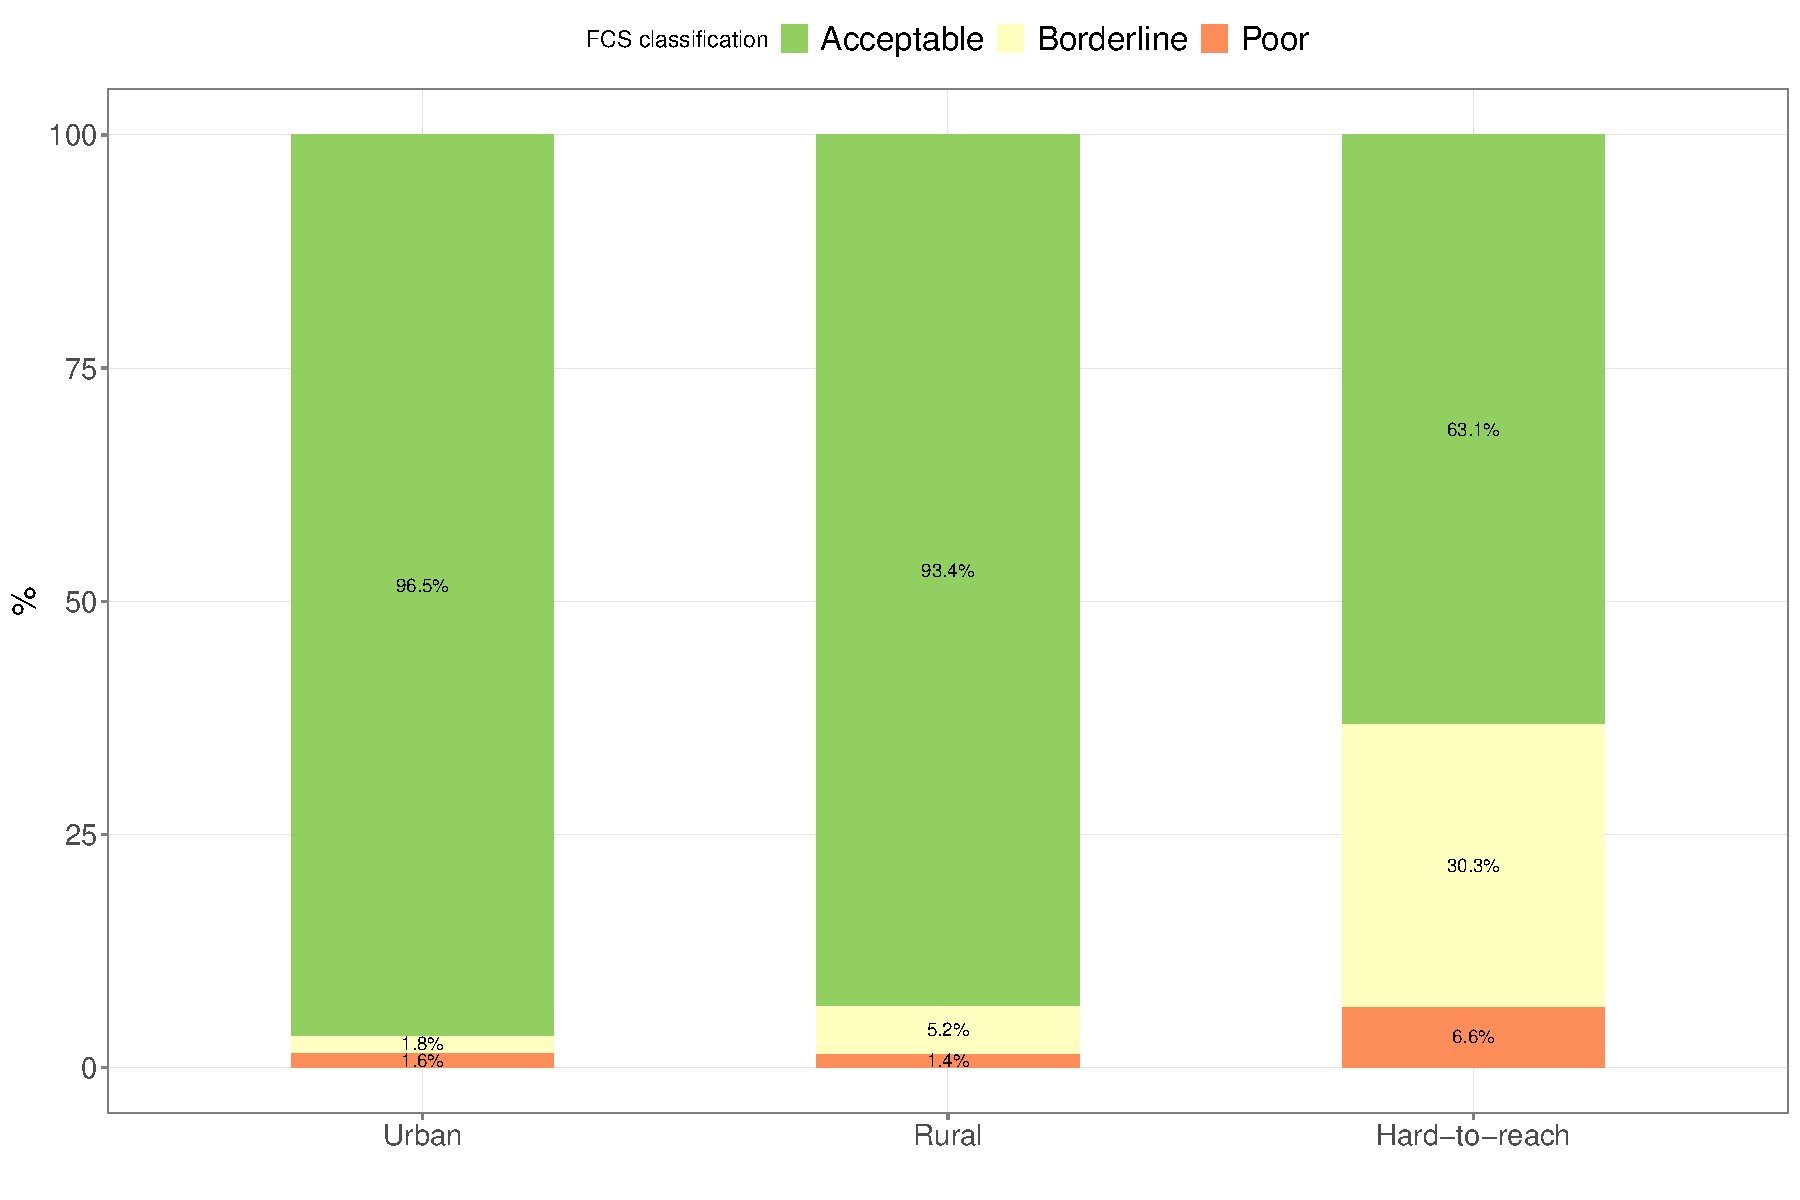
\includegraphics{kayinReport_files/figure-latex/fcs1plot-1} 

}

\caption{Food consumption score classification by location type}\label{fig:fcs1plot}
\end{figure}

\begin{figure}[H]

{\centering 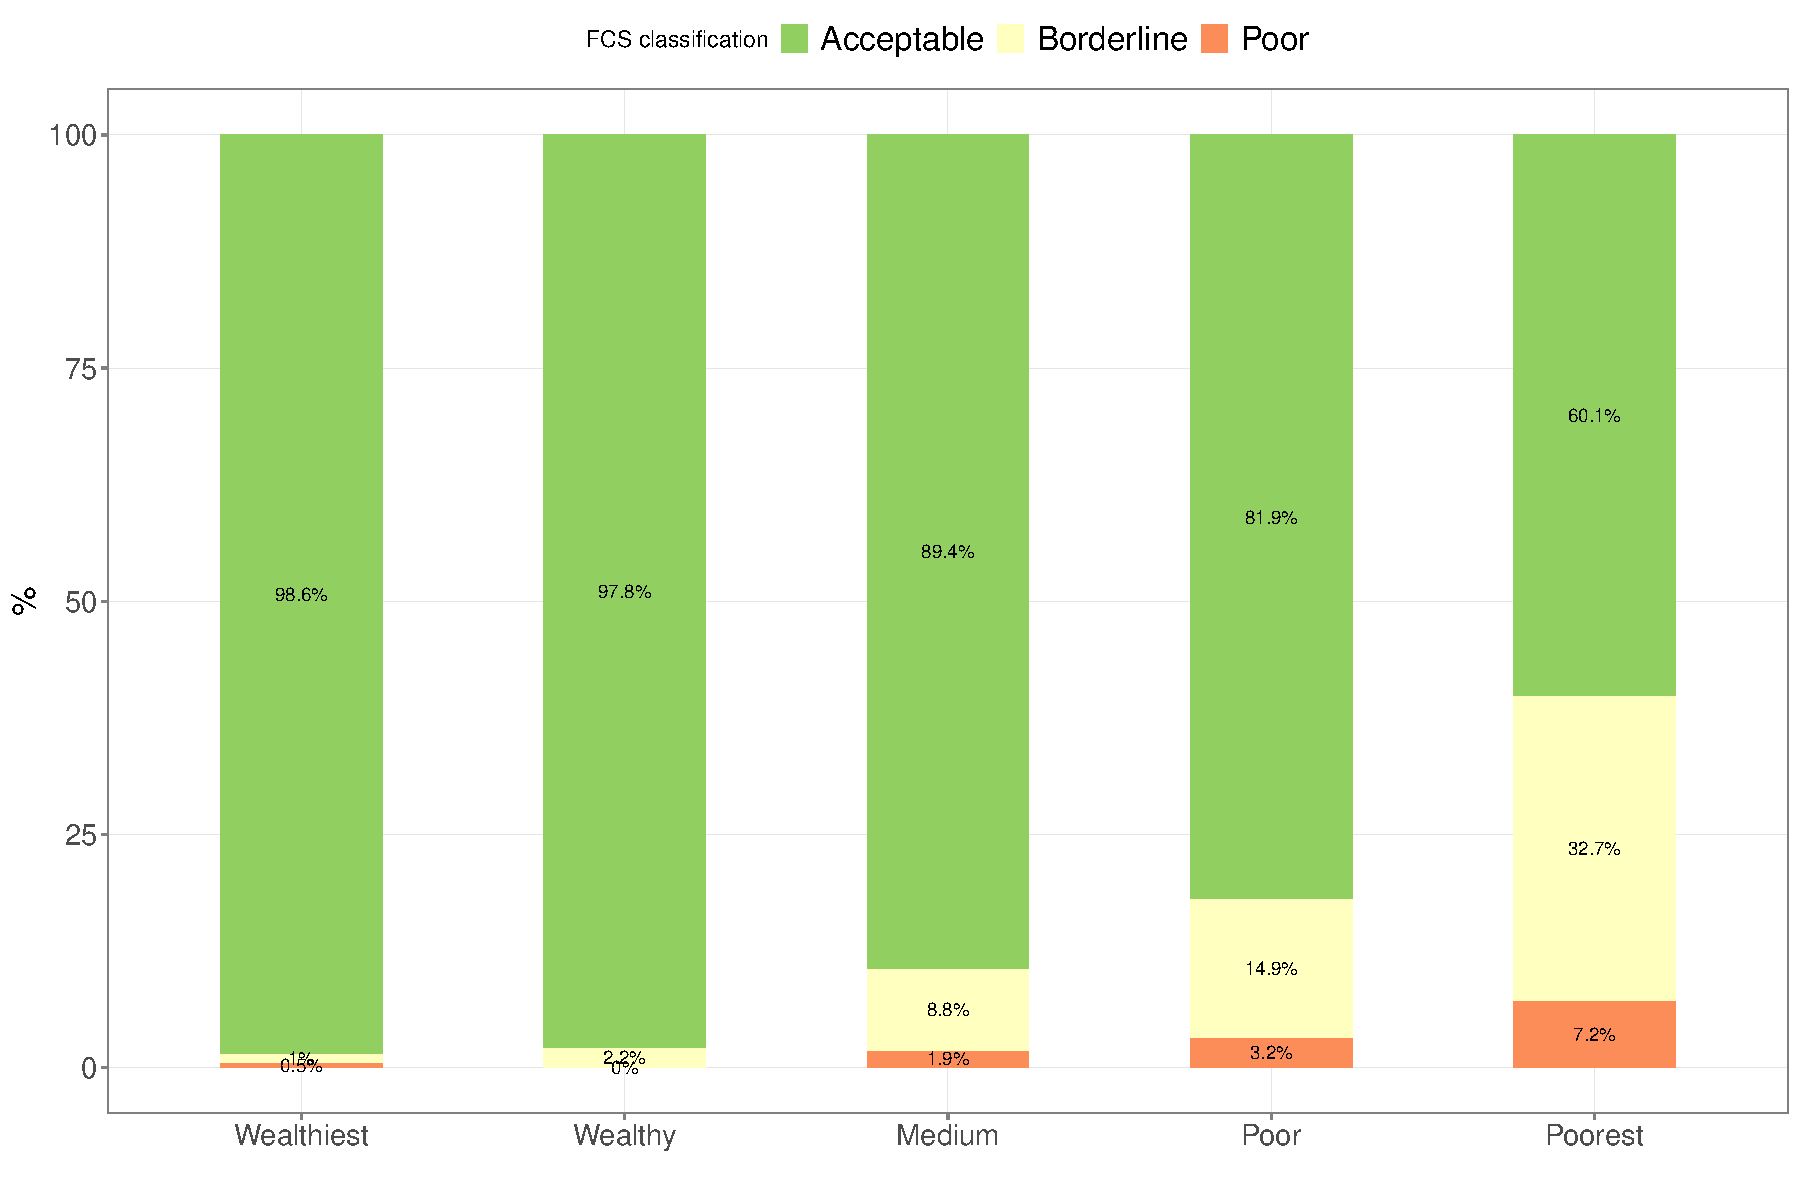
\includegraphics{kayinReport_files/figure-latex/fcs2plot-1} 

}

\caption{Food consumption score classification by wealth quintiles}\label{fig:fcs2plot}
\end{figure}

\newpage

\hypertarget{fcsn-results}{%
\subsubsection{Food consumption score - nutrition}\label{fcsn-results}}

Household consumption of vitamin A-, protein- and heme iron-rich foods indicates the quality of the household diet. In Kayin State, frequency of consumption of these nutrient-rich foods is generally high with vitamin A- and protein-rich foods consumed more frequently than heme iron-rich foods. In addition, the frequency of household consumption of these nutrients is influenced by geographic location and wealth. Vitamin A-rich foods are consumed at least daily by 81.8\% and 73.5\% of households in urban and rural areas respectively and then drops to as low as 58.3\% in hard-to-reach areas (see Figure \ref{fig:fcsn1plot}). The same decreasing pattern of frequency of vitamin A-rich foods consumption is noted when households are grouped by wealth quintiles with the majority of the wealthiest and the wealthy consuming vitamin A-rich foods at least daily while poor and poorest households consumed vitamin A-rich foods at least daily only 71\% and 48.4\% of the times respectively (see Figure \ref{fig:fcsn2plot}). This same trend is noted with frequency of household consumption of protein-rich foods (see Figure \ref{fig:fcsn3plot} and Figure \ref{fig:fcsn4plot}) and frequency of household consumption of heme iron-rich foods (see Figure \ref{fig:fcsn5plot} and \ref{fig:fcsn6plot}) but to a lesser magnitude.

\begin{table}[H]

\caption{\label{tab:fcsn1table}Food consumption score - nutrition}
\centering
\fontsize{9}{11}\selectfont
\begin{tabular}[t]{>{\bfseries}l>{\bfseries}l>{\ttfamily}r>{\ttfamily}r>{\ttfamily}r>{\ttfamily}r>{\ttfamily}r>{\ttfamily}r>{\ttfamily}r>{\ttfamily}r>{\ttfamily}r}
\toprule
\multicolumn{2}{c}{ } & \multicolumn{3}{c}{Vitamin A-rich foods} & \multicolumn{3}{c}{Protein-rich foods} & \multicolumn{3}{c}{Heme iron-rich foods} \\
\cmidrule(l{3pt}r{3pt}){3-5} \cmidrule(l{3pt}r{3pt}){6-8} \cmidrule(l{3pt}r{3pt}){9-11}
 &  & \makecell[c]{Never\\(\%)} & \makecell[c]{Sometimes\\(\%)} & \makecell[c]{At\\least\\daily\\(\%)} & \makecell[c]{Never\\(\%)} & \makecell[c]{Sometimes\\(\%)} & \makecell[c]{At\\least\\daily\\(\%)} & \makecell[c]{Never\\(\%)} & \makecell[c]{Sometimes\\(\%)} & \makecell[c]{At\\least\\daily\\(\%)}\\
\midrule
\addlinespace[0.3em]
\multicolumn{11}{l}{\textbf{Kayin}}\\
\addlinespace[0.3em]
\multicolumn{11}{l}{\textit{\textbf{Geographic}}}\\
\hspace{1em}\hspace{1em} & Rural & 4.6 & 21.9 & 73.5 & 1.4 & 20.2 & 78.4 & 5.2 & 46.4 & 48.4\\
\cmidrule{2-11}
\hspace{1em}\hspace{1em} & Urban & 1.8 & 16.4 & 81.8 & 1.8 & 8.8 & 89.4 & 2.3 & 44.6 & 53.1\\
\cmidrule{2-11}
\hspace{1em}\hspace{1em} & Hard-to-reach & 10.0 & 31.7 & 58.3 & 9.7 & 48.0 & 42.3 & 16.9 & 63.4 & 19.7\\
\cmidrule{2-11}
\addlinespace[0.3em]
\multicolumn{11}{l}{\textit{\textbf{Wealth}}}\\
\hspace{1em}\hspace{1em} & Wealthiest & 1.0 & 14.4 & 84.7 & 1.0 & 7.2 & 91.9 & 1.0 & 40.2 & 58.9\\
\cmidrule{2-11}
\hspace{1em}\hspace{1em} & Wealthy & 0.0 & 17.7 & 82.3 & 0.0 & 13.0 & 87.0 & 0.4 & 50.6 & 48.9\\
\cmidrule{2-11}
\hspace{1em}\hspace{1em} & Medium & 2.3 & 23.6 & 74.1 & 1.9 & 23.1 & 75.0 & 4.2 & 56.0 & 39.8\\
\cmidrule{2-11}
\hspace{1em}\hspace{1em} & Poor & 5.0 & 24.0 & 71.0 & 3.6 & 28.5 & 67.9 & 10.4 & 52.9 & 36.7\\
\cmidrule{2-11}
\hspace{1em}\hspace{1em} & Poorest & 15.2 & 36.3 & 48.4 & 11.7 & 52.9 & 35.4 & 20.2 & 58.3 & 21.5\\
\bottomrule
\end{tabular}
\end{table}

\begin{figure}[H]

{\centering 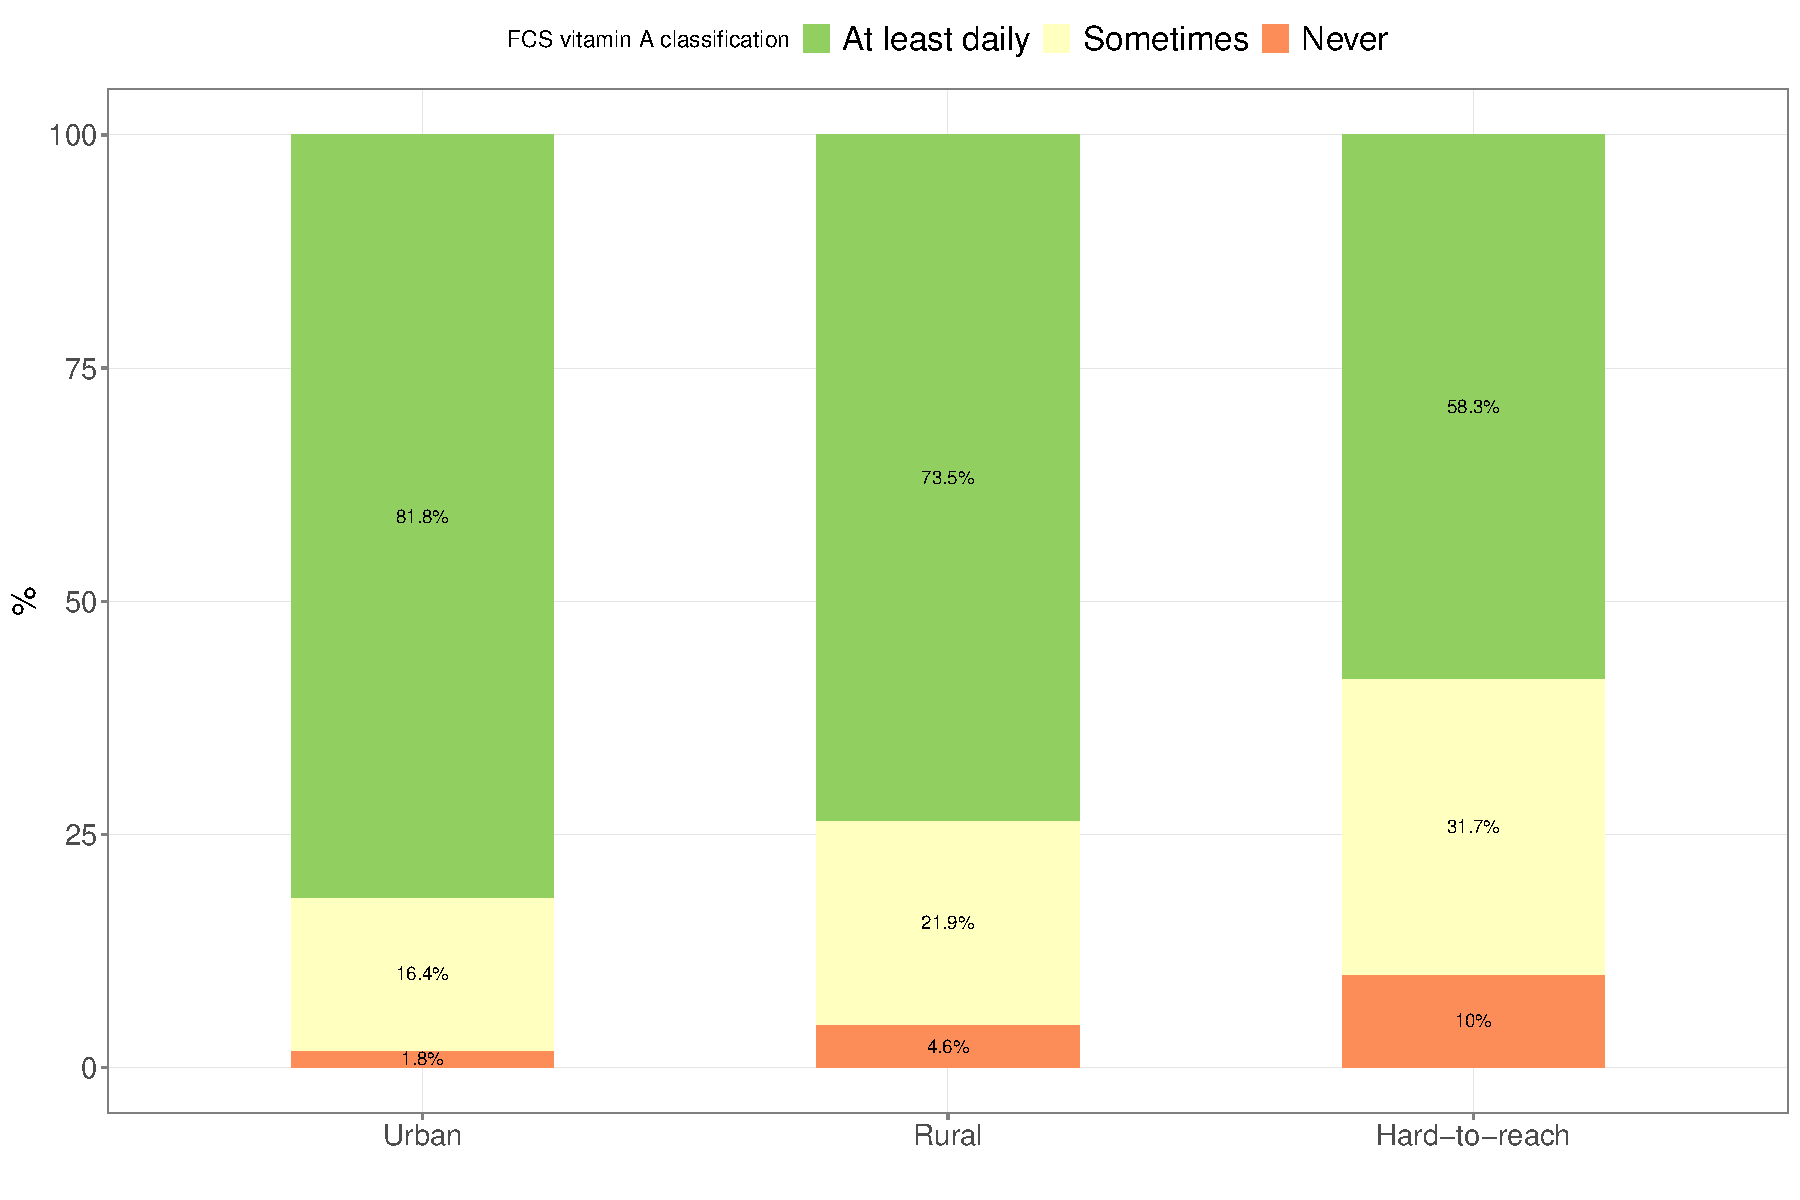
\includegraphics{kayinReport_files/figure-latex/fcsn1plot-1} 

}

\caption{Vitamin A food consumption score classification by location type}\label{fig:fcsn1plot}
\end{figure}

\begin{figure}[H]

{\centering 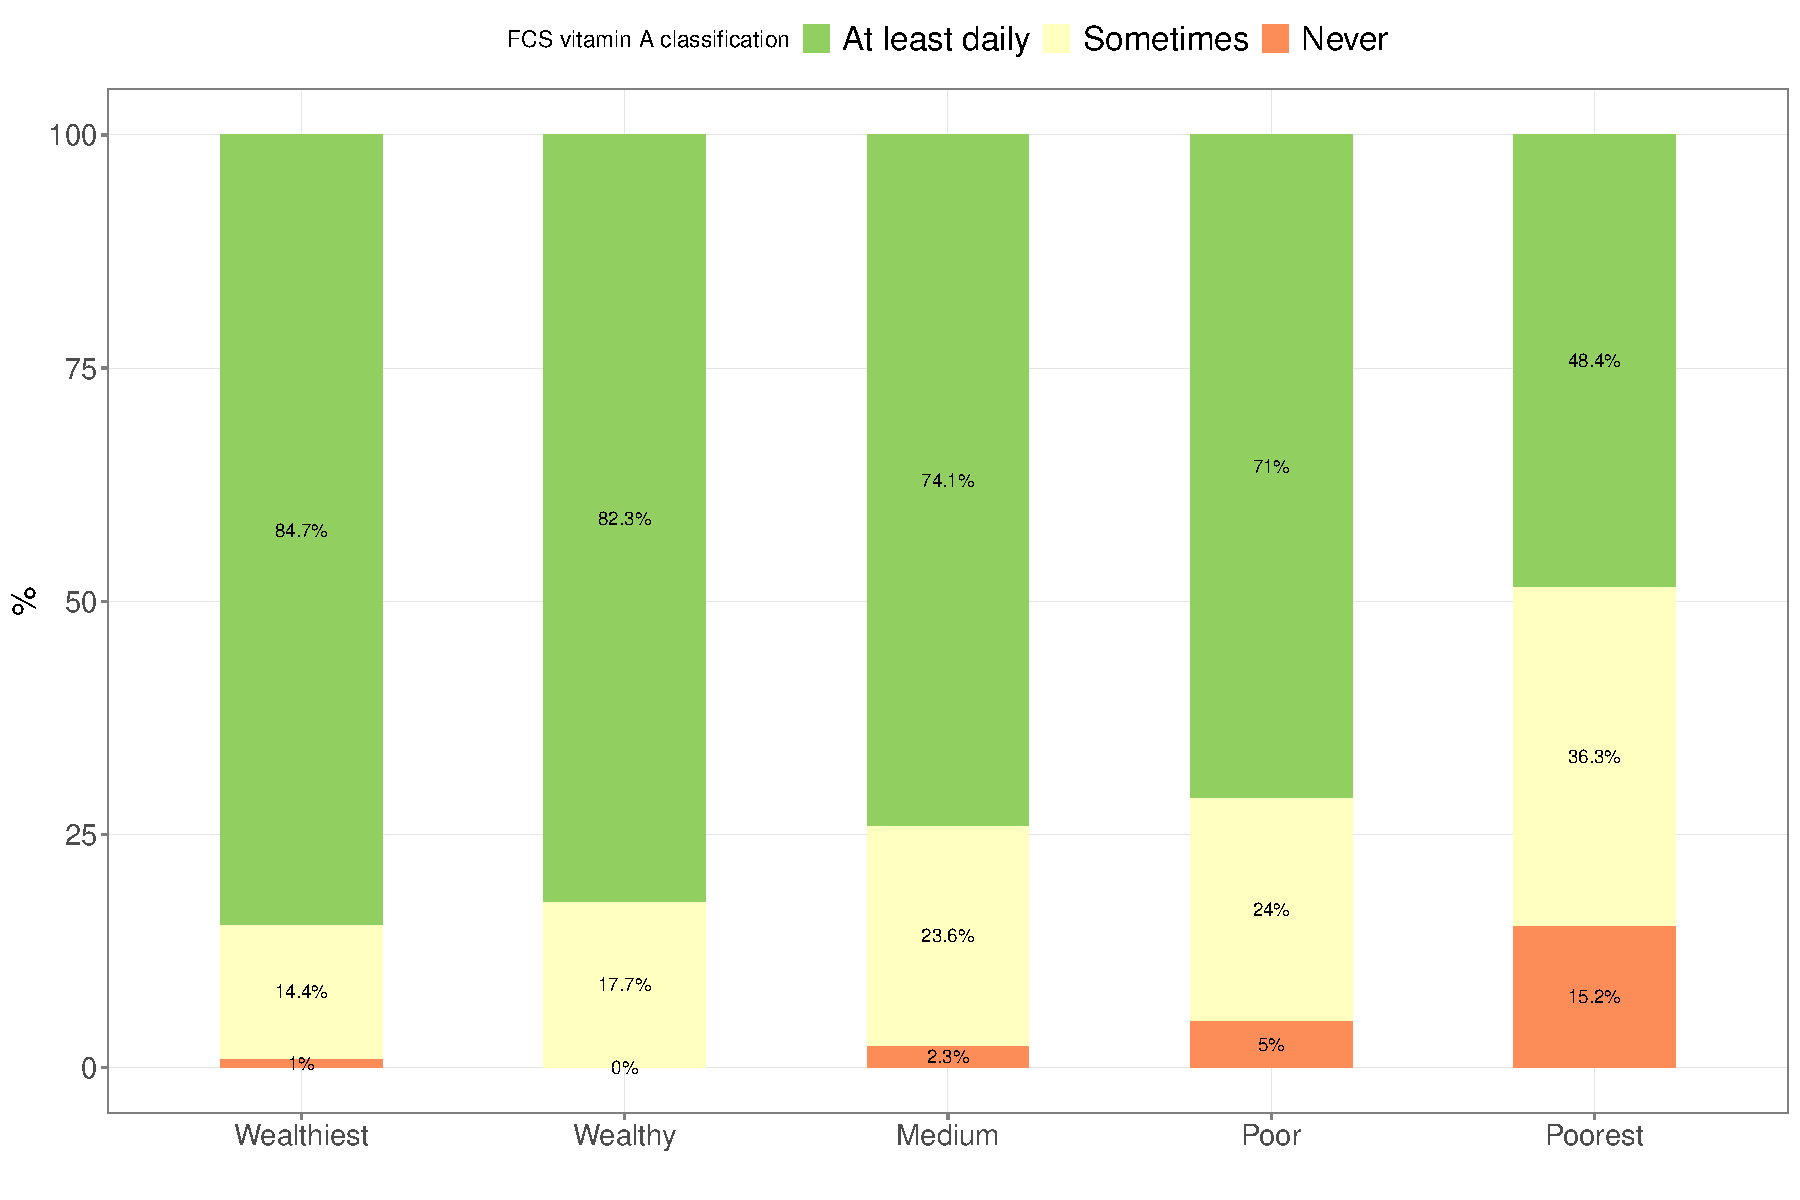
\includegraphics{kayinReport_files/figure-latex/fcsn2plot-1} 

}

\caption{Vitamin A food consumption score classification by wealth quintiles}\label{fig:fcsn2plot}
\end{figure}

\begin{figure}[H]

{\centering 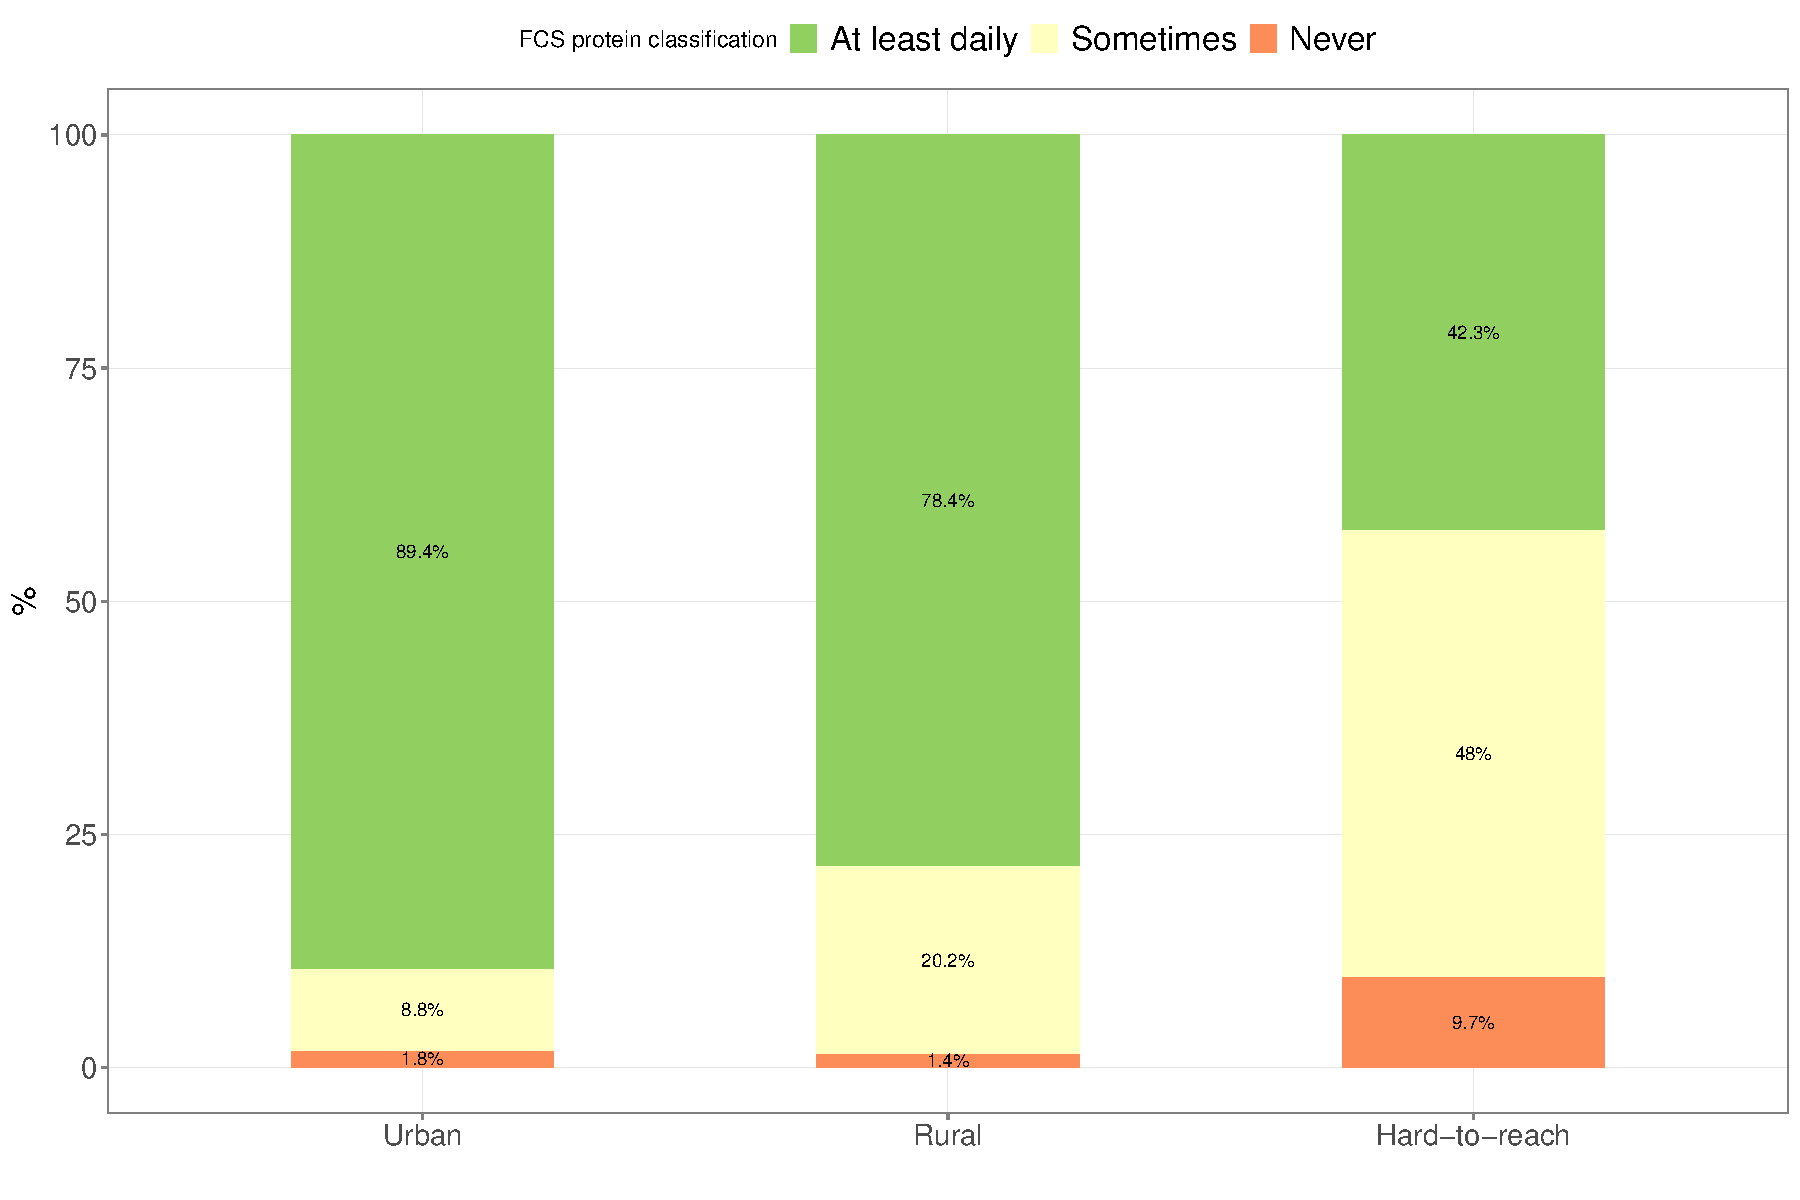
\includegraphics{kayinReport_files/figure-latex/fcsn3plot-1} 

}

\caption{Protein food consumption score classification by location type}\label{fig:fcsn3plot}
\end{figure}

\begin{figure}[H]

{\centering 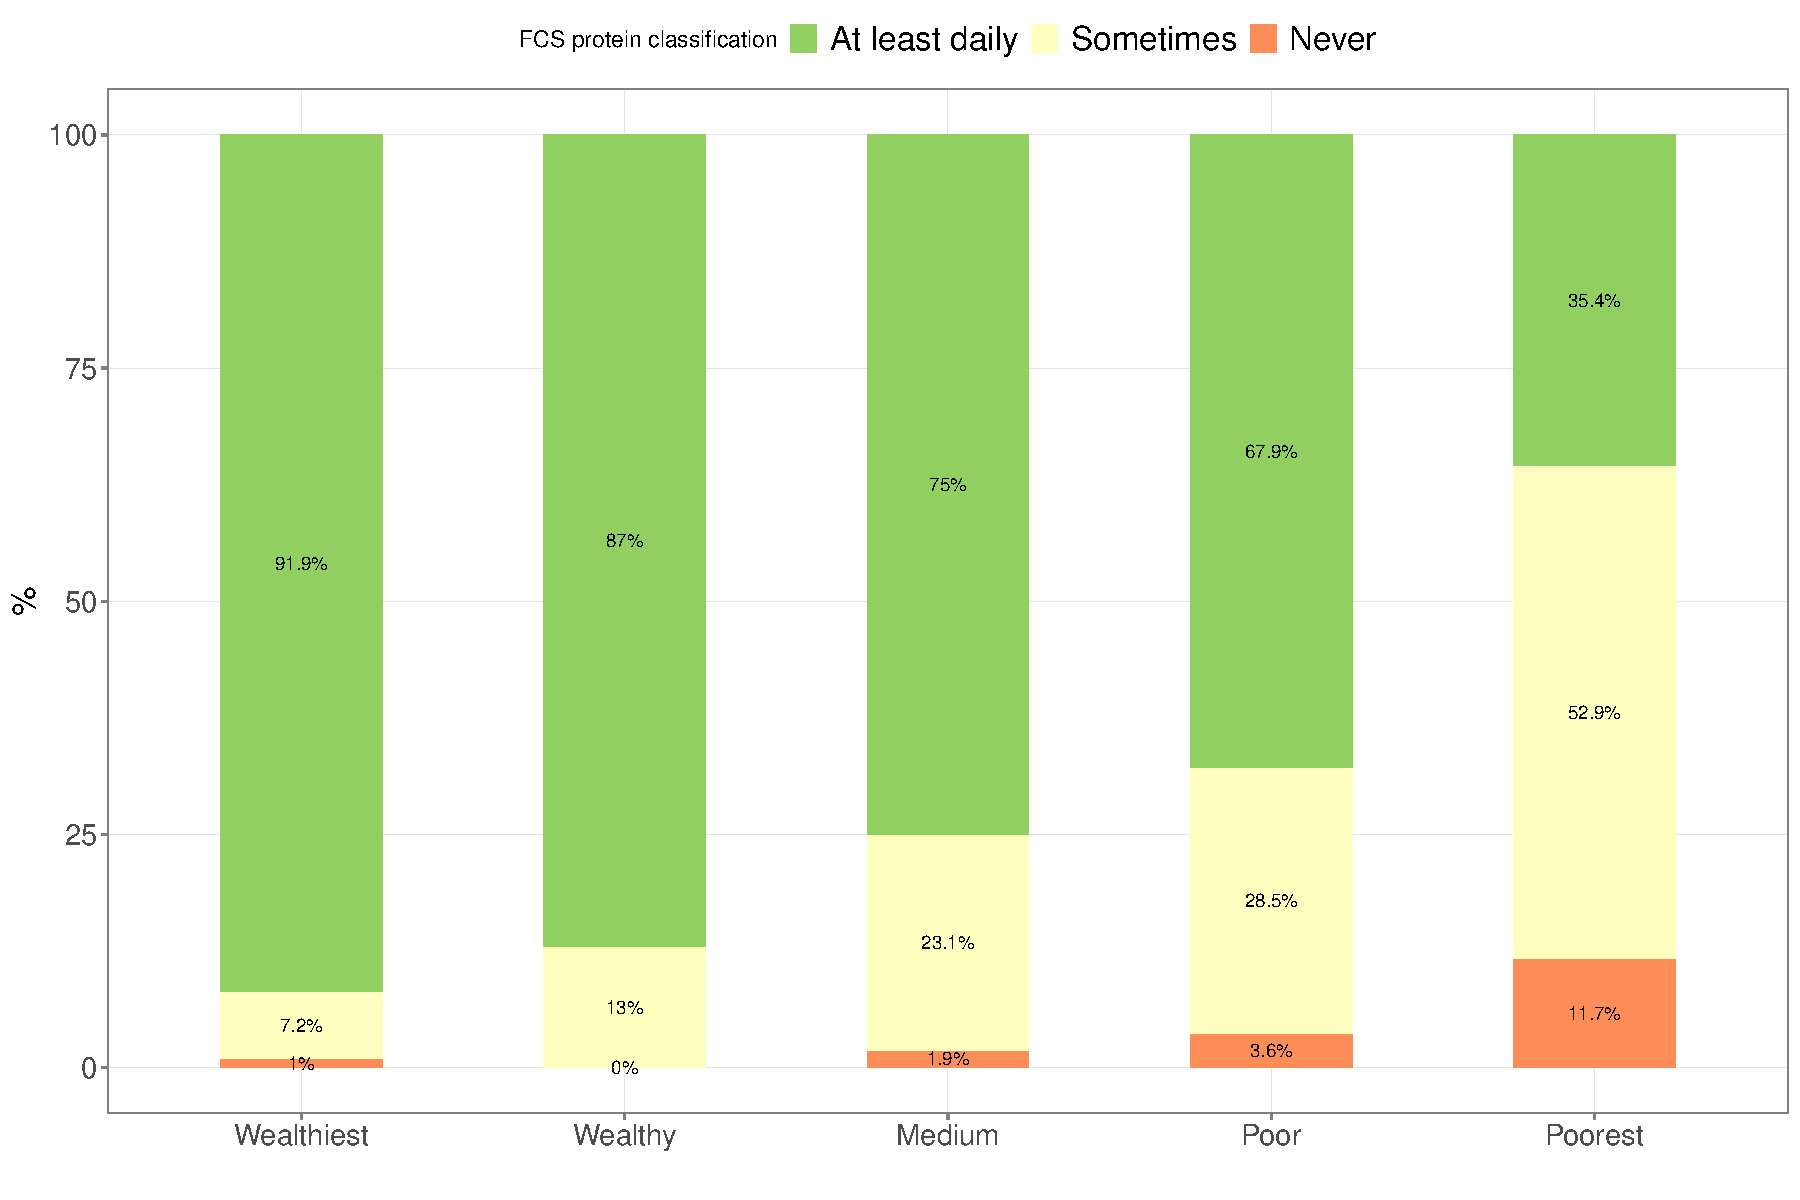
\includegraphics{kayinReport_files/figure-latex/fcsn4plot-1} 

}

\caption{Protein food consumption score classification by wealth quintiles}\label{fig:fcsn4plot}
\end{figure}

\begin{figure}[H]

{\centering 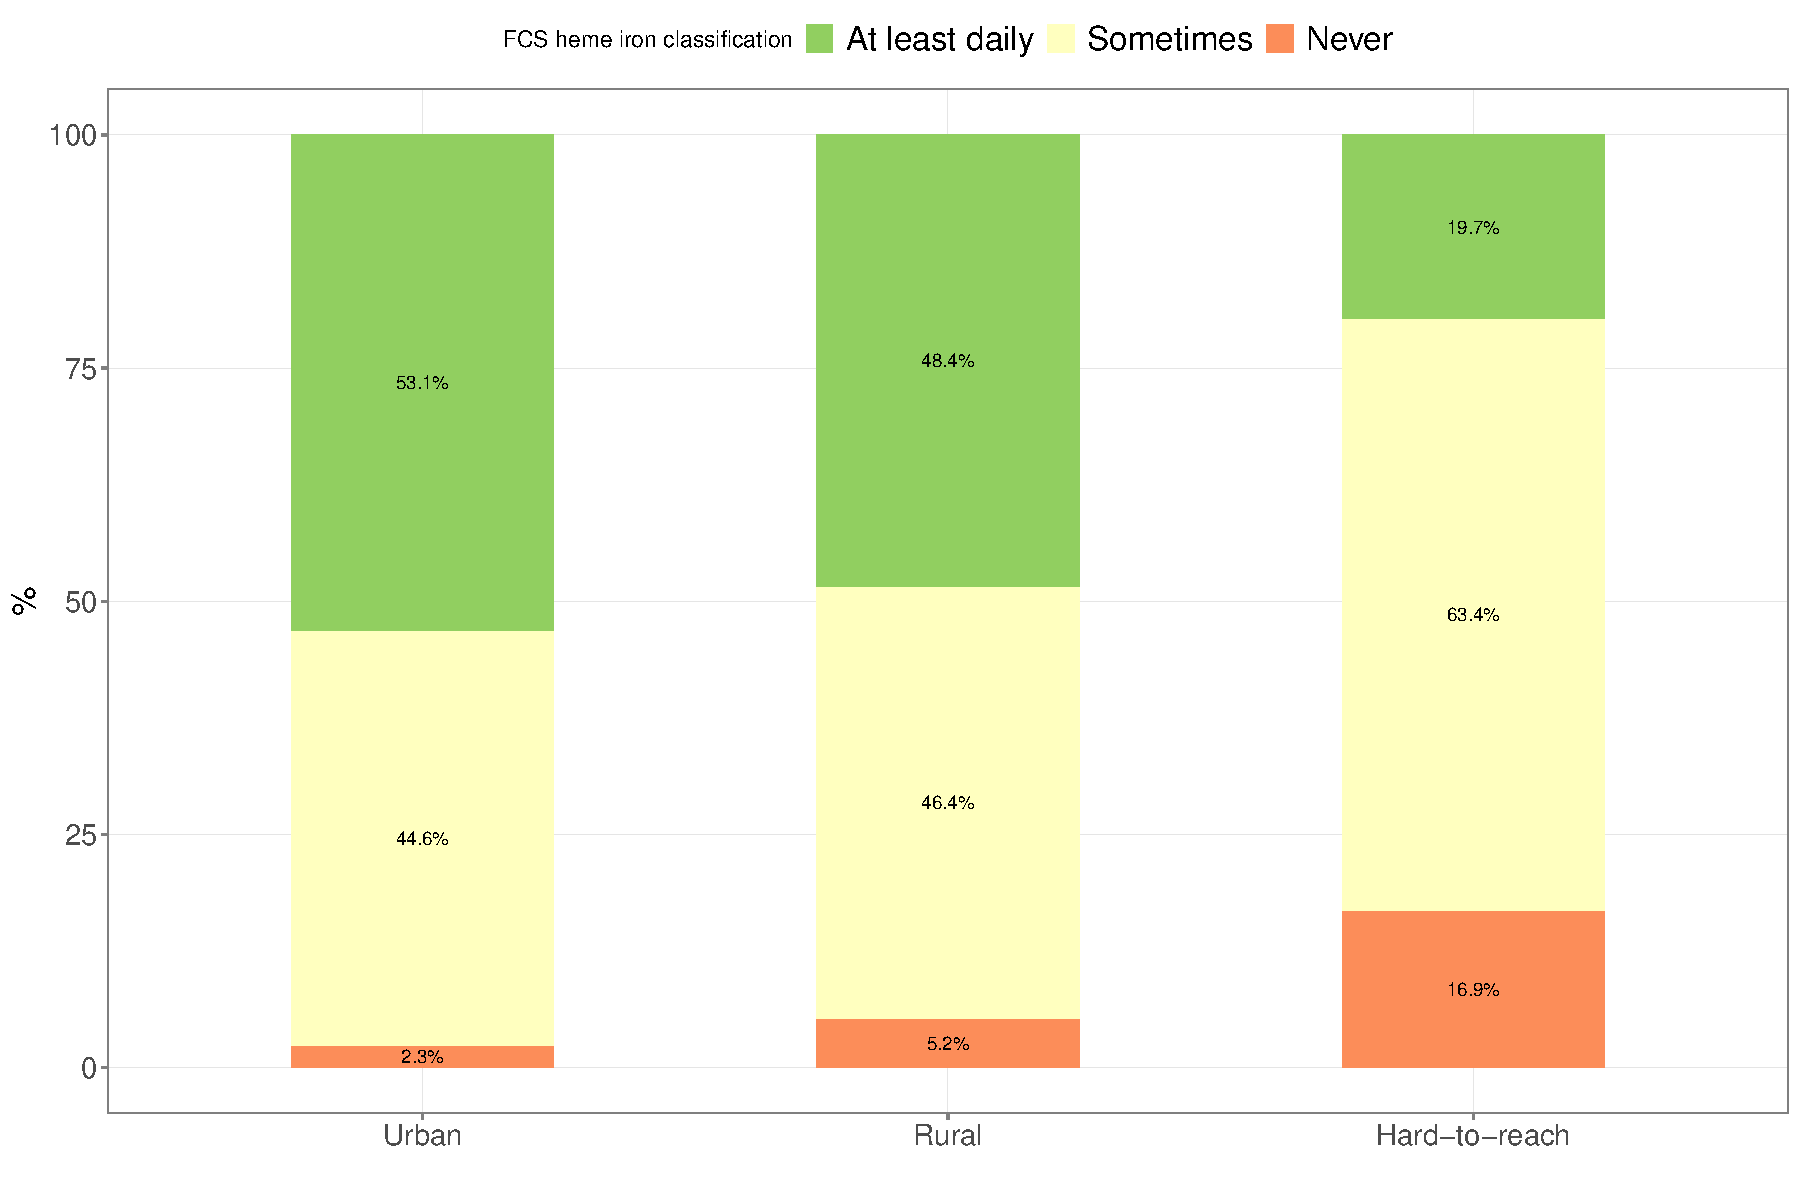
\includegraphics{kayinReport_files/figure-latex/fcsn5plot-1} 

}

\caption{Heme iron-rich food consumption score classification by location type}\label{fig:fcsn5plot}
\end{figure}

\begin{figure}[H]

{\centering 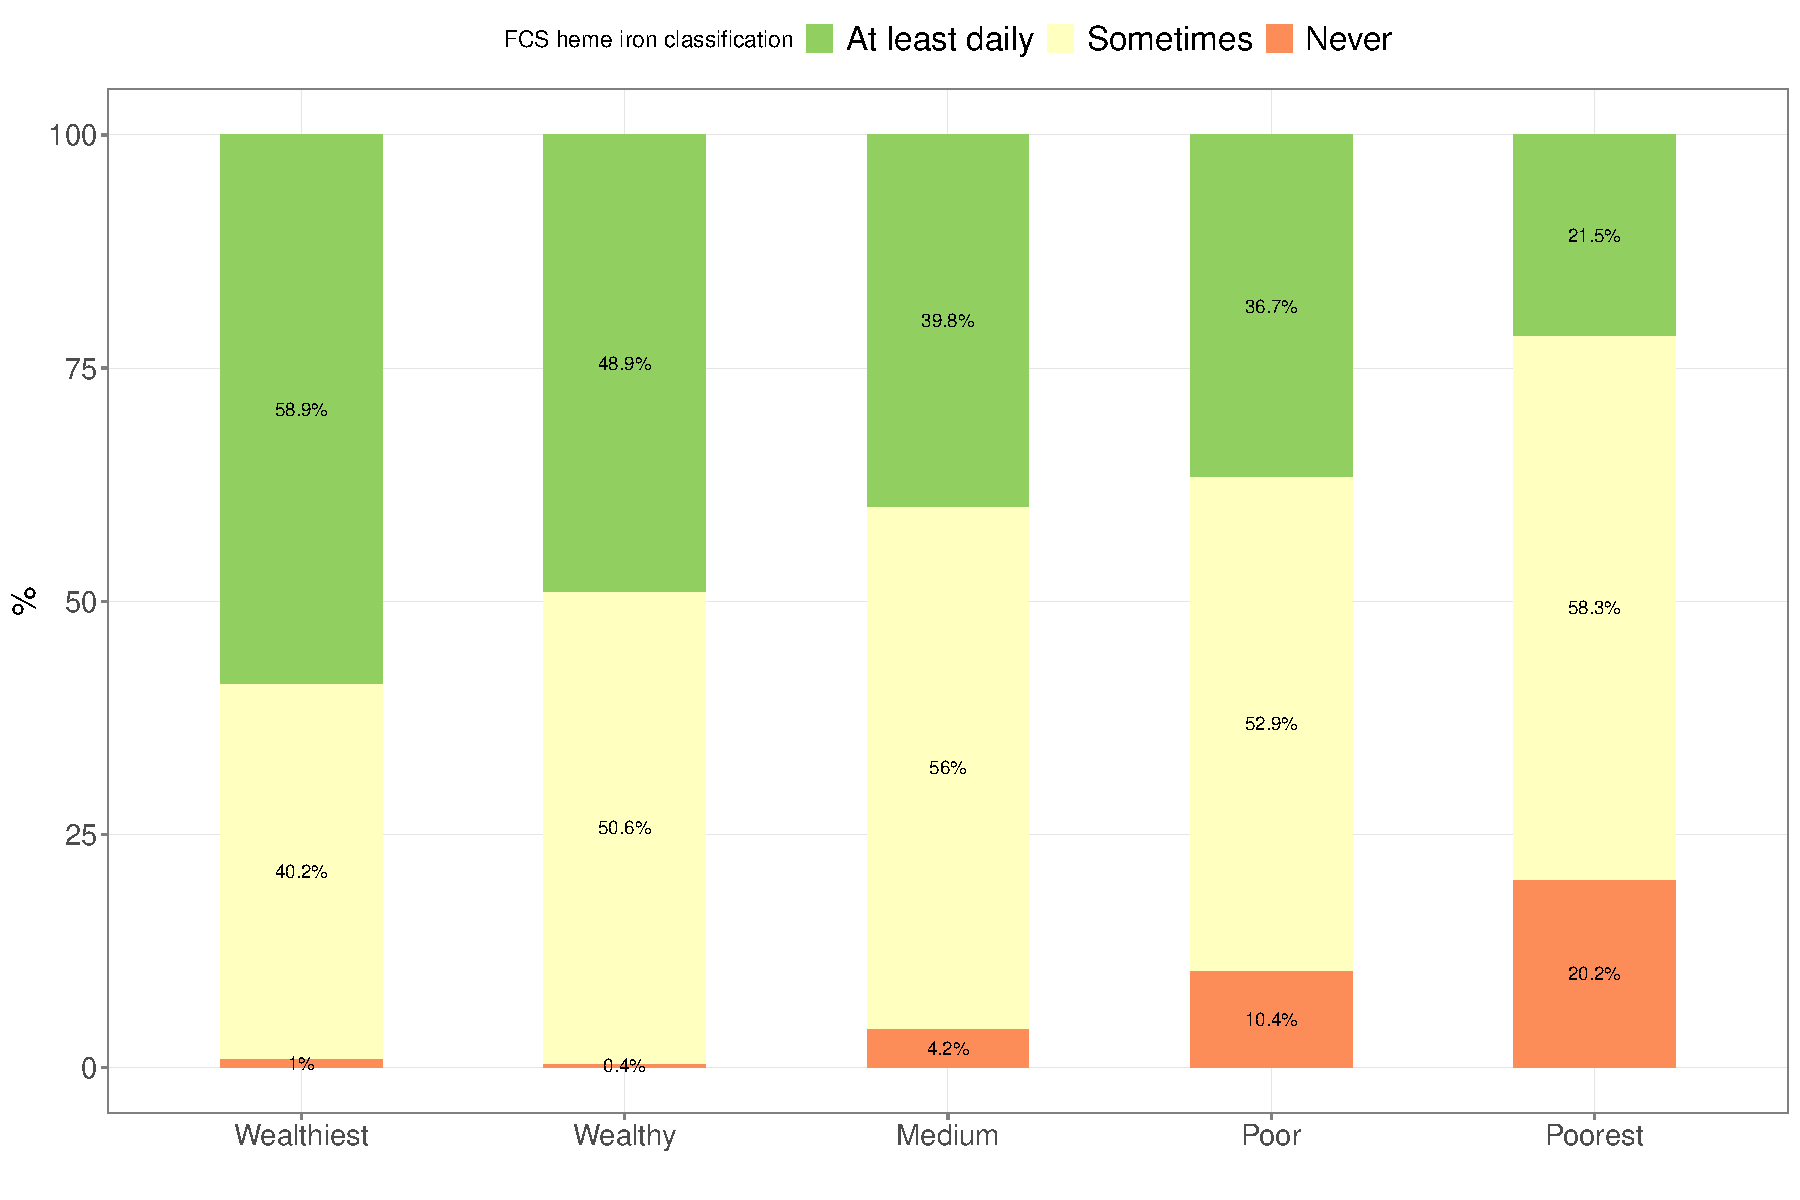
\includegraphics{kayinReport_files/figure-latex/fcsn6plot-1} 

}

\caption{Protein food consumption score classification by wealth quintiles}\label{fig:fcsn6plot}
\end{figure}

\hypertarget{csi-results}{%
\subsubsection{Coping strategies index}\label{csi-results}}

\hypertarget{ccsi-results}{%
\paragraph{Consumption-based coping strategies index}\label{ccsi-results}}

\begin{table}[H]

\caption{\label{tab:ccsi1table}Consumption-based Coping Strategies Index}
\centering
\fontsize{12}{14}\selectfont
\begin{tabular}[t]{>{\bfseries}l>{\bfseries}l>{\ttfamily}r}
\toprule
 &  & Mean CSI\\
\midrule
\addlinespace[0.3em]
\multicolumn{3}{l}{\textbf{Kayin}}\\
\addlinespace[0.3em]
\multicolumn{3}{l}{\textit{\textbf{Geographic}}}\\
\hspace{1em}\hspace{1em} & Rural & 3.0\\
\cmidrule{2-3}
\hspace{1em}\hspace{1em} & Urban & 2.8\\
\cmidrule{2-3}
\hspace{1em}\hspace{1em} & Hard-to-reach & 3.2\\
\cmidrule{2-3}
\addlinespace[0.3em]
\multicolumn{3}{l}{\textit{\textbf{Wealth}}}\\
\hspace{1em}\hspace{1em} & Wealthiest & 2.0\\
\cmidrule{2-3}
\hspace{1em}\hspace{1em} & Wealthy & 2.1\\
\cmidrule{2-3}
\hspace{1em}\hspace{1em} & Medium & 2.7\\
\cmidrule{2-3}
\hspace{1em}\hspace{1em} & Poor & 3.3\\
\cmidrule{2-3}
\hspace{1em}\hspace{1em} & Poorest & 5.2\\
\bottomrule
\end{tabular}
\end{table}

Households in Kayin state are employing very few consumption-based coping strategies (see Table \ref{tab:ccsi1table}). Use of consumption-based coping strategies is higher in households in hard-to-reach areas (3.2) compared to households in urban and rural areas (2.8 and 3 respectively) as shown in Figure \ref{fig:ccsi1plot} and Figure \ref{fig:ccsi2plot}.

\newpage

\begin{figure}[H]

{\centering 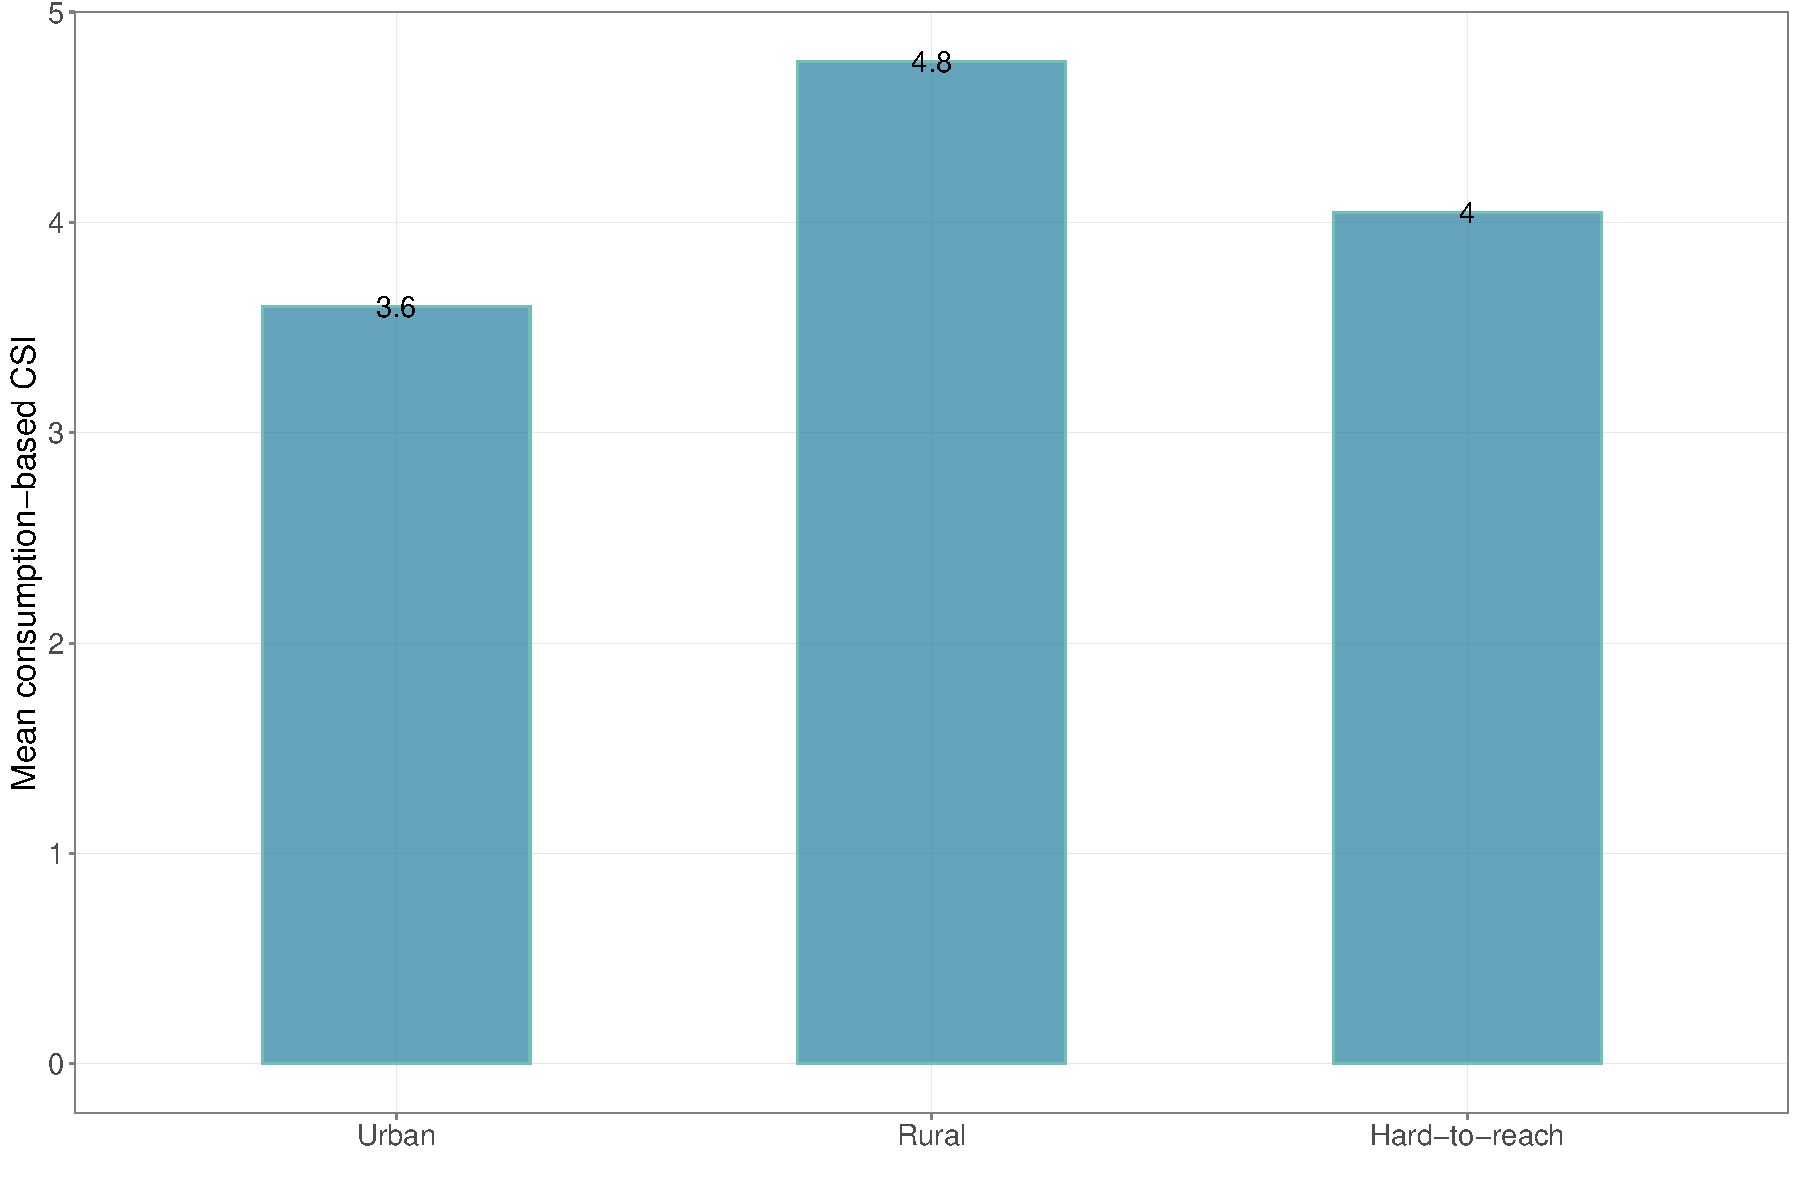
\includegraphics{kayinReport_files/figure-latex/ccsi1plot-1} 

}

\caption{Consumption-based coping strategies index by location type}\label{fig:ccsi1plot}
\end{figure}

\begin{figure}[H]

{\centering 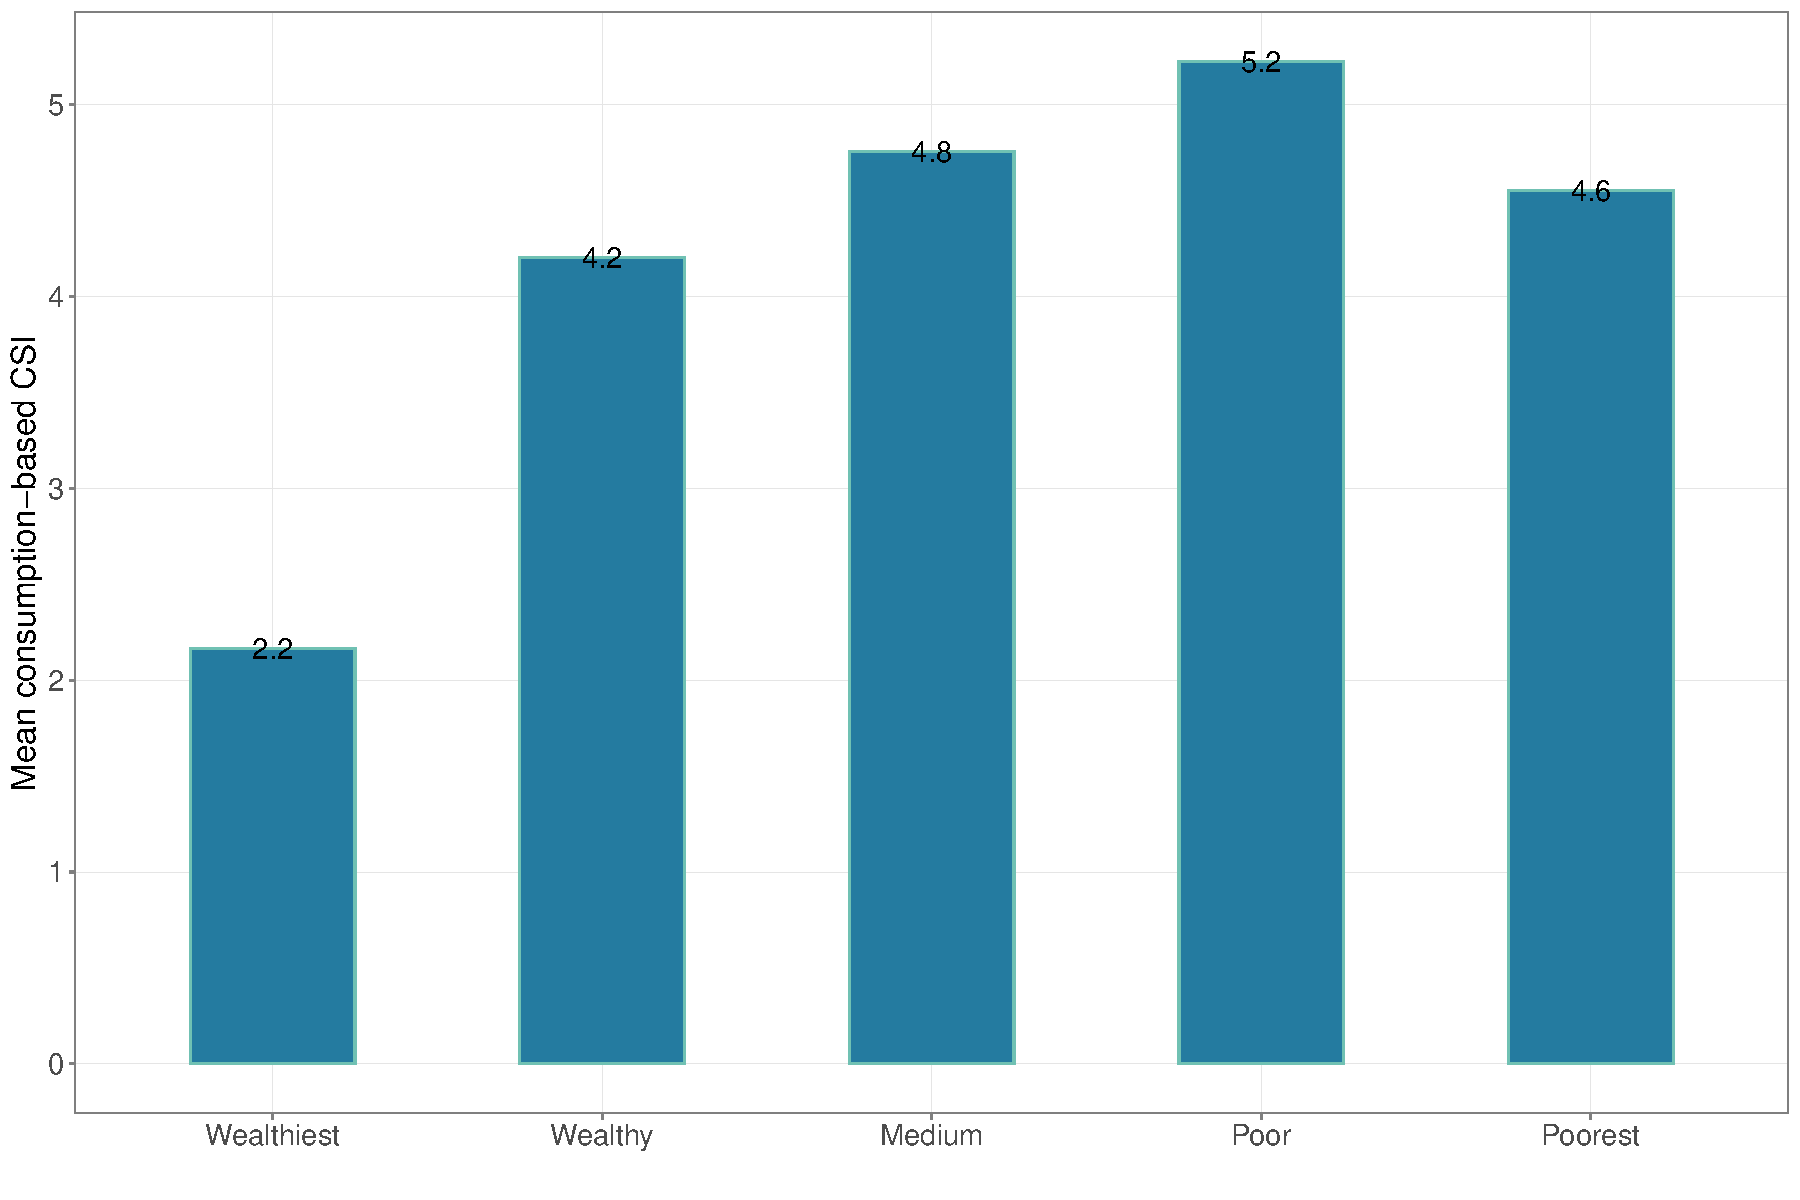
\includegraphics{kayinReport_files/figure-latex/ccsi2plot-1} 

}

\caption{Consumption-based coping strategies index by wealth quintiles}\label{fig:ccsi2plot}
\end{figure}

\hypertarget{lcsi-results}{%
\paragraph{Livelihood-based coping strategies index}\label{lcsi-results}}

The use of a few consumption-based coping strategies by households in Kayin state can be partly explained by close to 50\% of households being relatively food secure in that they are not requiring longer-term livelihoods-based coping strategies. However, up to 40\% of households across Kayin State utilise stress type of livelihoods coping strategies in the longer term (see Table \ref{tab:lcsi1Table}). There is a seeming geographical and wealth gradient for livelihoods-based coping strategies. A higher proportion of households in hard-to-reach areas are relatively food secure and a lower proportion of households in hard-to-reach areas are in stress (see Figure \ref{fig:lcsi1plot}). A similar trend can be found across wealth classes in that higher proportion of food secure households and lower proportion of households in stress or in crisis were observed among poorer households compared to wealthier households (see Figure \ref{fig:lcsi2plot}).

\begin{table}[H]

\caption{\label{tab:lcsi1table}Livelihoods-based coping strategies index}
\centering
\fontsize{12}{14}\selectfont
\begin{tabular}[t]{>{\bfseries}l>{\bfseries}l>{\ttfamily}r>{\ttfamily}r>{\ttfamily}r>{\ttfamily}r}
\toprule
 &  & \makecell[c]{Secure\\(\%)} & \makecell[c]{Stress\\(\%)} & \makecell[c]{Crisis\\(\%)} & \makecell[c]{Emergency\\(\%)}\\
\midrule
\addlinespace[0.3em]
\multicolumn{6}{l}{\textbf{Kayin}}\\
\addlinespace[0.3em]
\multicolumn{6}{l}{\textit{\textbf{Geographic}}}\\
\hspace{1em}\hspace{1em} & Rural & 46.7 & 39.8 & 11.5 & 2.0\\
\cmidrule{2-6}
\hspace{1em}\hspace{1em} & Urban & 39.7 & 44.6 & 14.8 & 0.9\\
\cmidrule{2-6}
\hspace{1em}\hspace{1em} & Hard-to-reach & 60.6 & 32.0 & 5.4 & 2.0\\
\cmidrule{2-6}
\addlinespace[0.3em]
\multicolumn{6}{l}{\textit{\textbf{Wealth}}}\\
\hspace{1em}\hspace{1em} & Wealthiest & 46.9 & 43.5 & 8.6 & 1.0\\
\cmidrule{2-6}
\hspace{1em}\hspace{1em} & Wealthy & 40.7 & 45.0 & 13.4 & 0.9\\
\cmidrule{2-6}
\hspace{1em}\hspace{1em} & Medium & 47.2 & 38.0 & 13.9 & 0.9\\
\cmidrule{2-6}
\hspace{1em}\hspace{1em} & Poor & 49.3 & 37.1 & 10.9 & 2.7\\
\cmidrule{2-6}
\hspace{1em}\hspace{1em} & Poorest & 55.6 & 33.6 & 8.1 & 2.7\\
\bottomrule
\end{tabular}
\end{table}

\newpage

\begin{figure}[H]

{\centering 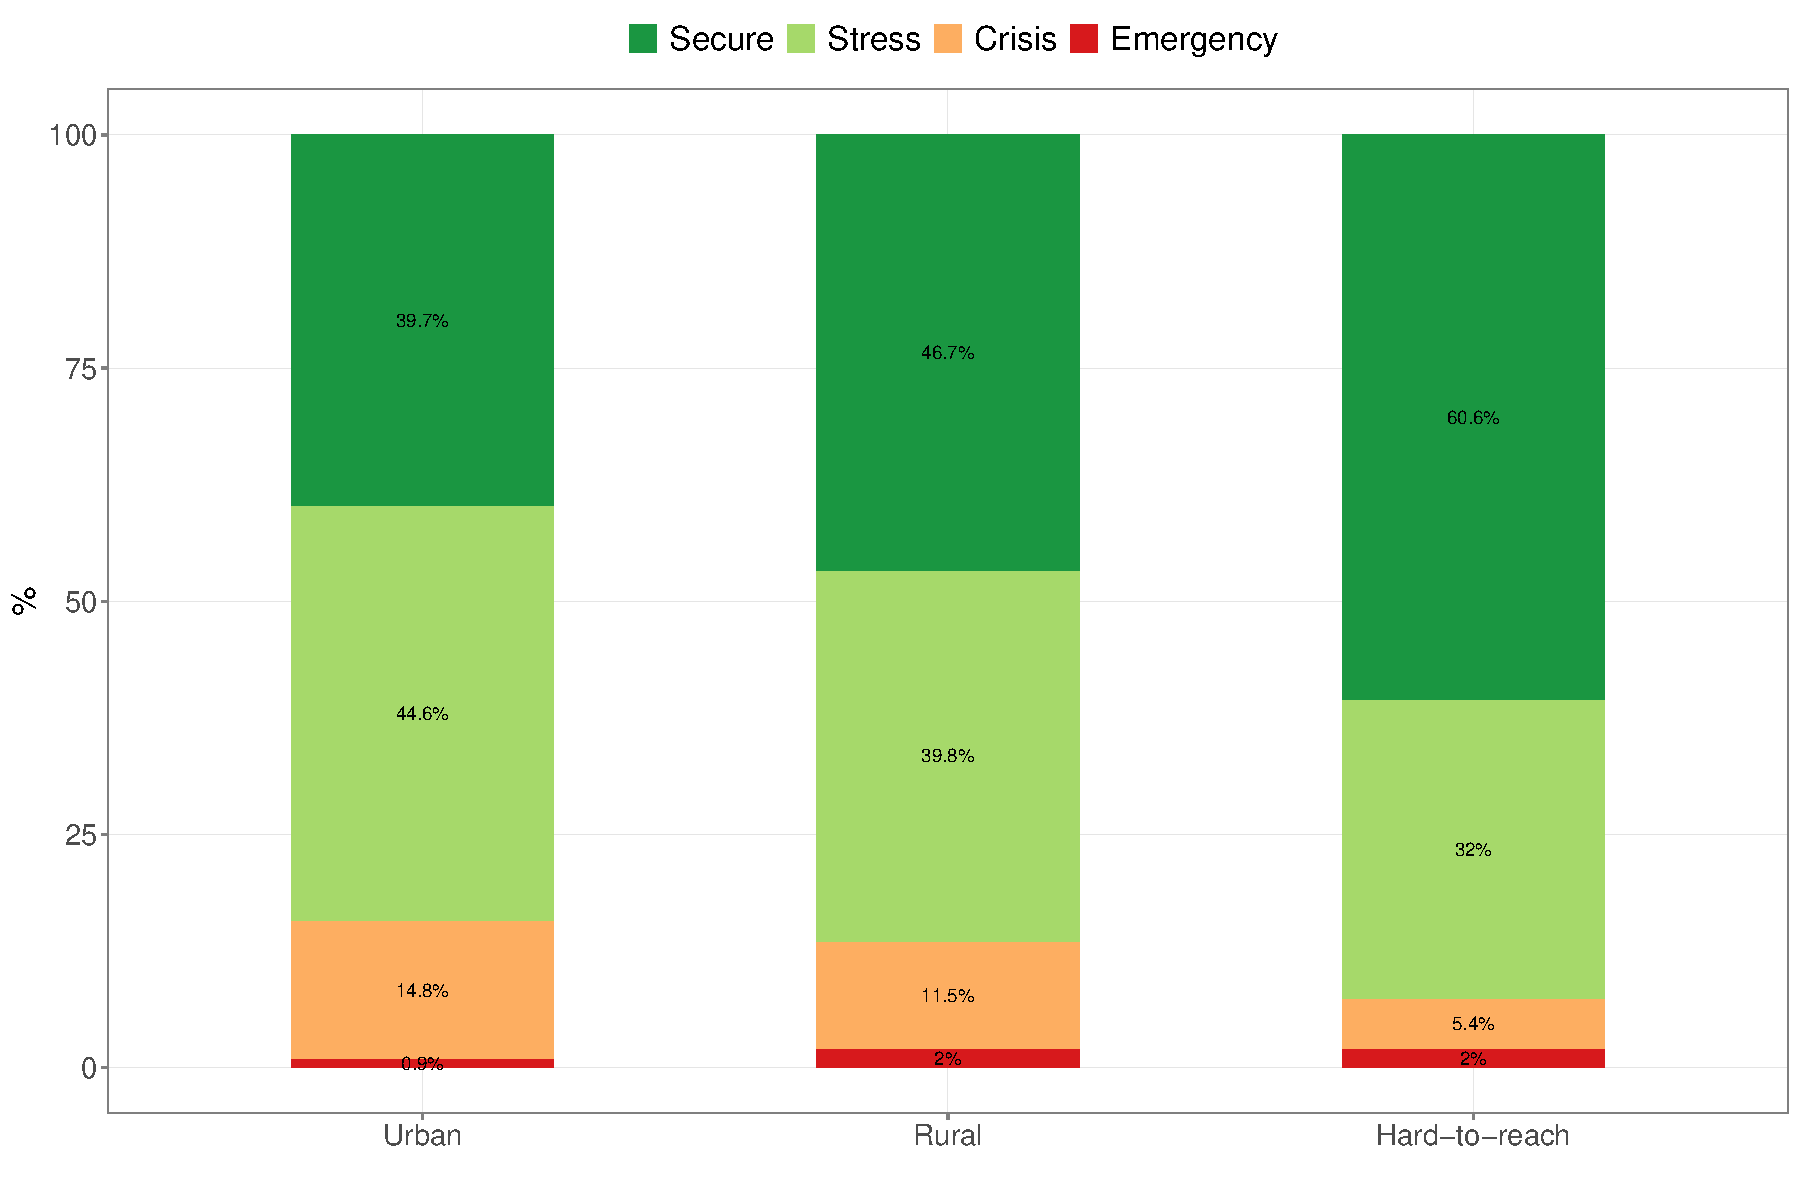
\includegraphics{kayinReport_files/figure-latex/lcsi1plot-1} 

}

\caption{Livelihoods-based coping strategies index by location type}\label{fig:lcsi1plot}
\end{figure}

\begin{figure}[H]

{\centering 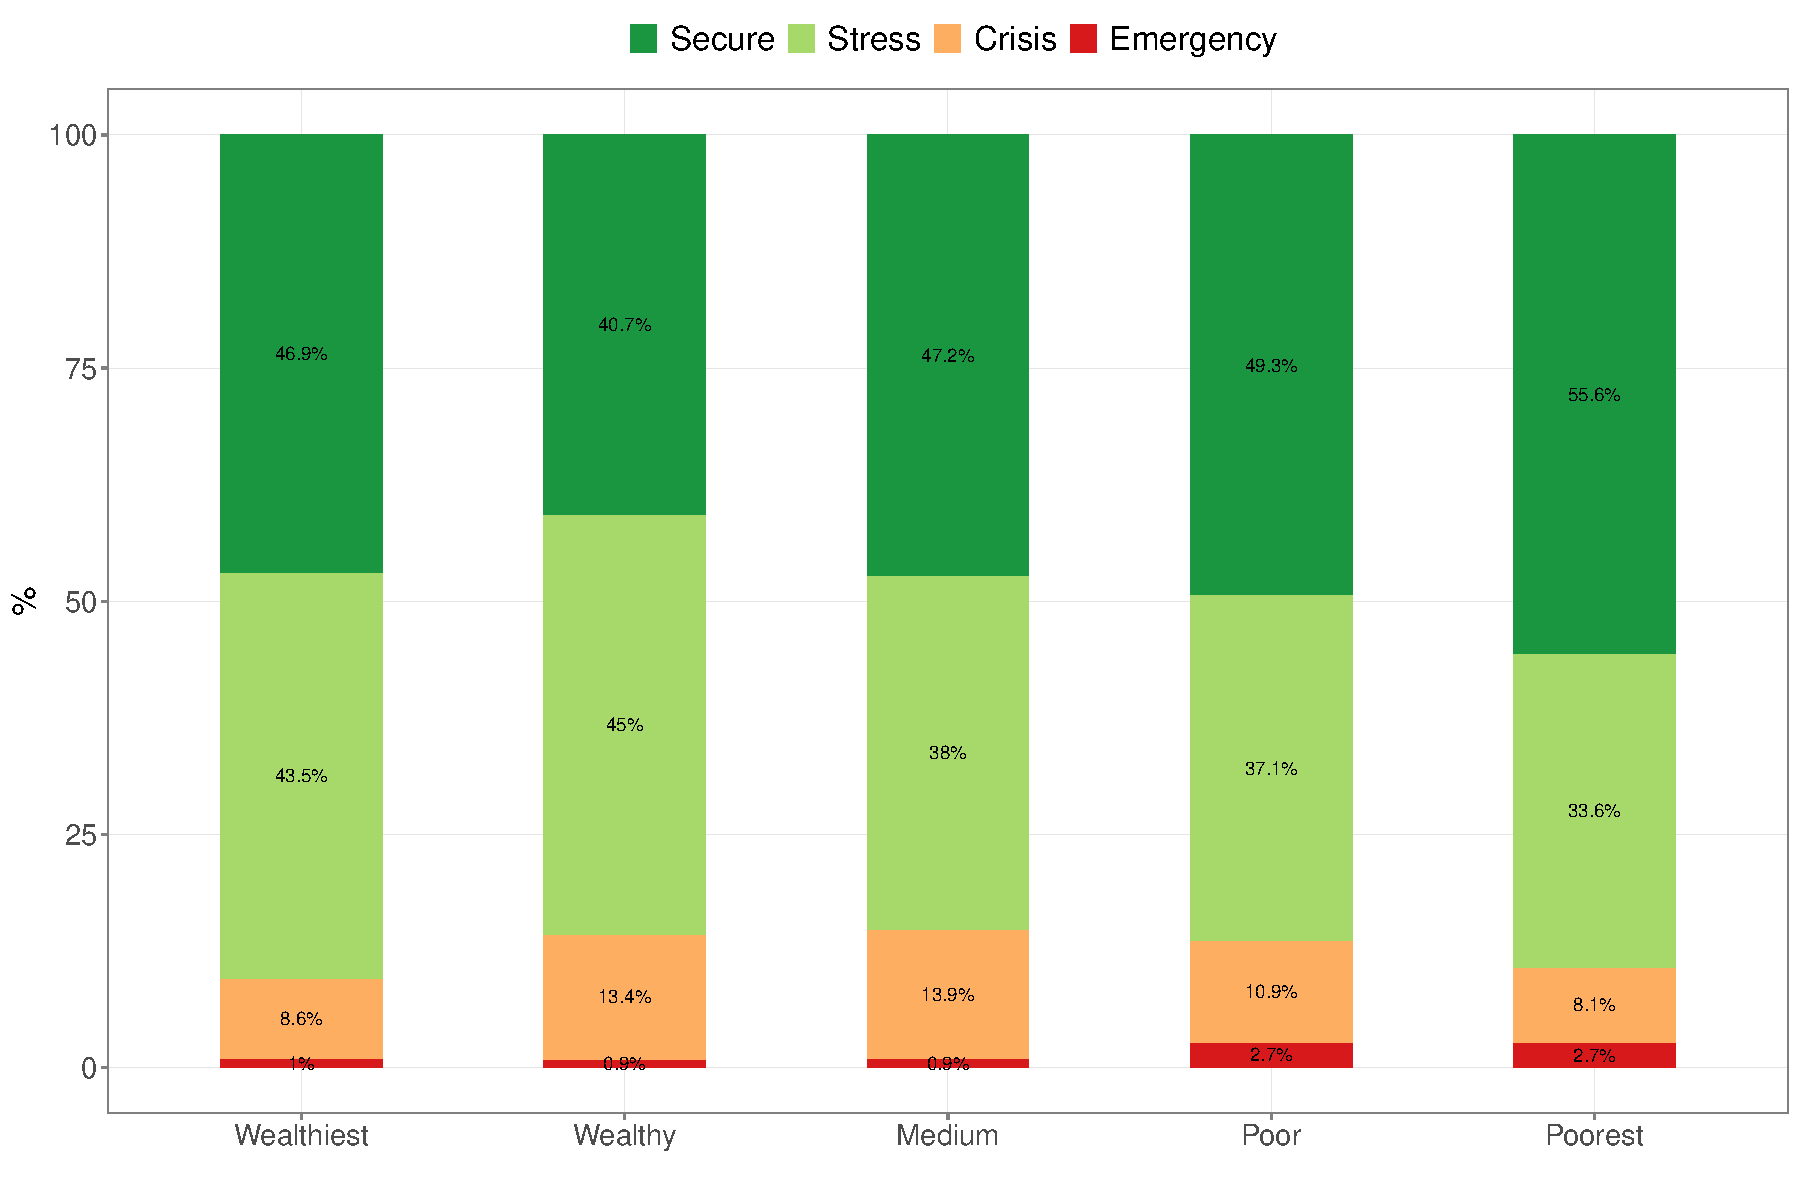
\includegraphics{kayinReport_files/figure-latex/lcsi2plot-1} 

}

\caption{Livelihoods-based coping strategies index by wealth quintiles}\label{fig:lcsi2plot}
\end{figure}

\hypertarget{hfes-results}{%
\subsubsection{Household food expenditure share}\label{hfes-results}}

Majority of households accross Kayin state have low food insecurity (see Table \ref{tab:hfes2table}) based on household food expenditure share (HFES). However, there are pockets of households in mostly hard-to-reach areas and households who are poor and poorest that are highly food insecure or vulnerable (see Figure \ref{fig:hfesScatterPlot1} and Figure \ref{fig:hfesScatterPlot2}).

\begin{table}[H]

\caption{\label{tab:hfes2table}Household food expenditure share}
\centering
\fontsize{12}{14}\selectfont
\begin{tabular}[t]{>{\bfseries}l>{\bfseries}l>{\ttfamily}r>{\ttfamily}r>{\ttfamily}r>{\ttfamily}r}
\toprule
\multicolumn{2}{c}{ } & \multicolumn{4}{c}{Food Insecurity by HFES} \\
\cmidrule(l{3pt}r{3pt}){3-6}
 &  & \makecell[c]{Vulnerable\\(\%)} & \makecell[c]{High\\(\%)} & \makecell[c]{Medium\\(\%)} & \makecell[c]{Low\\(\%)}\\
\midrule
\addlinespace[0.3em]
\multicolumn{6}{l}{\textbf{Kayin}}\\
\addlinespace[0.3em]
\multicolumn{6}{l}{\textit{\textbf{Geographic}}}\\
\hspace{1em}\hspace{1em} & Rural & 1.2 & 0.3 & 0.0 & 98.6\\
\cmidrule{2-6}
\hspace{1em}\hspace{1em} & Urban & 0.2 & 0.2 & 0.0 & 99.5\\
\cmidrule{2-6}
\hspace{1em}\hspace{1em} & Hard-to-reach & 1.1 & 1.7 & 1.4 & 95.7\\
\cmidrule{2-6}
\addlinespace[0.3em]
\multicolumn{6}{l}{\textit{\textbf{Wealth}}}\\
\hspace{1em}\hspace{1em} & Wealthiest & 0.0 & 0.0 & 0.0 & 100.0\\
\cmidrule{2-6}
\hspace{1em}\hspace{1em} & Wealthy & 0.0 & 0.0 & 0.0 & 100.0\\
\cmidrule{2-6}
\hspace{1em}\hspace{1em} & Medium & 1.4 & 1.4 & 0.0 & 97.2\\
\cmidrule{2-6}
\hspace{1em}\hspace{1em} & Poor & 1.4 & 0.5 & 0.5 & 97.7\\
\cmidrule{2-6}
\hspace{1em}\hspace{1em} & Poorest & 1.3 & 1.8 & 1.8 & 95.1\\
\bottomrule
\end{tabular}
\end{table}

\newpage

\begin{figure}[H]

{\centering 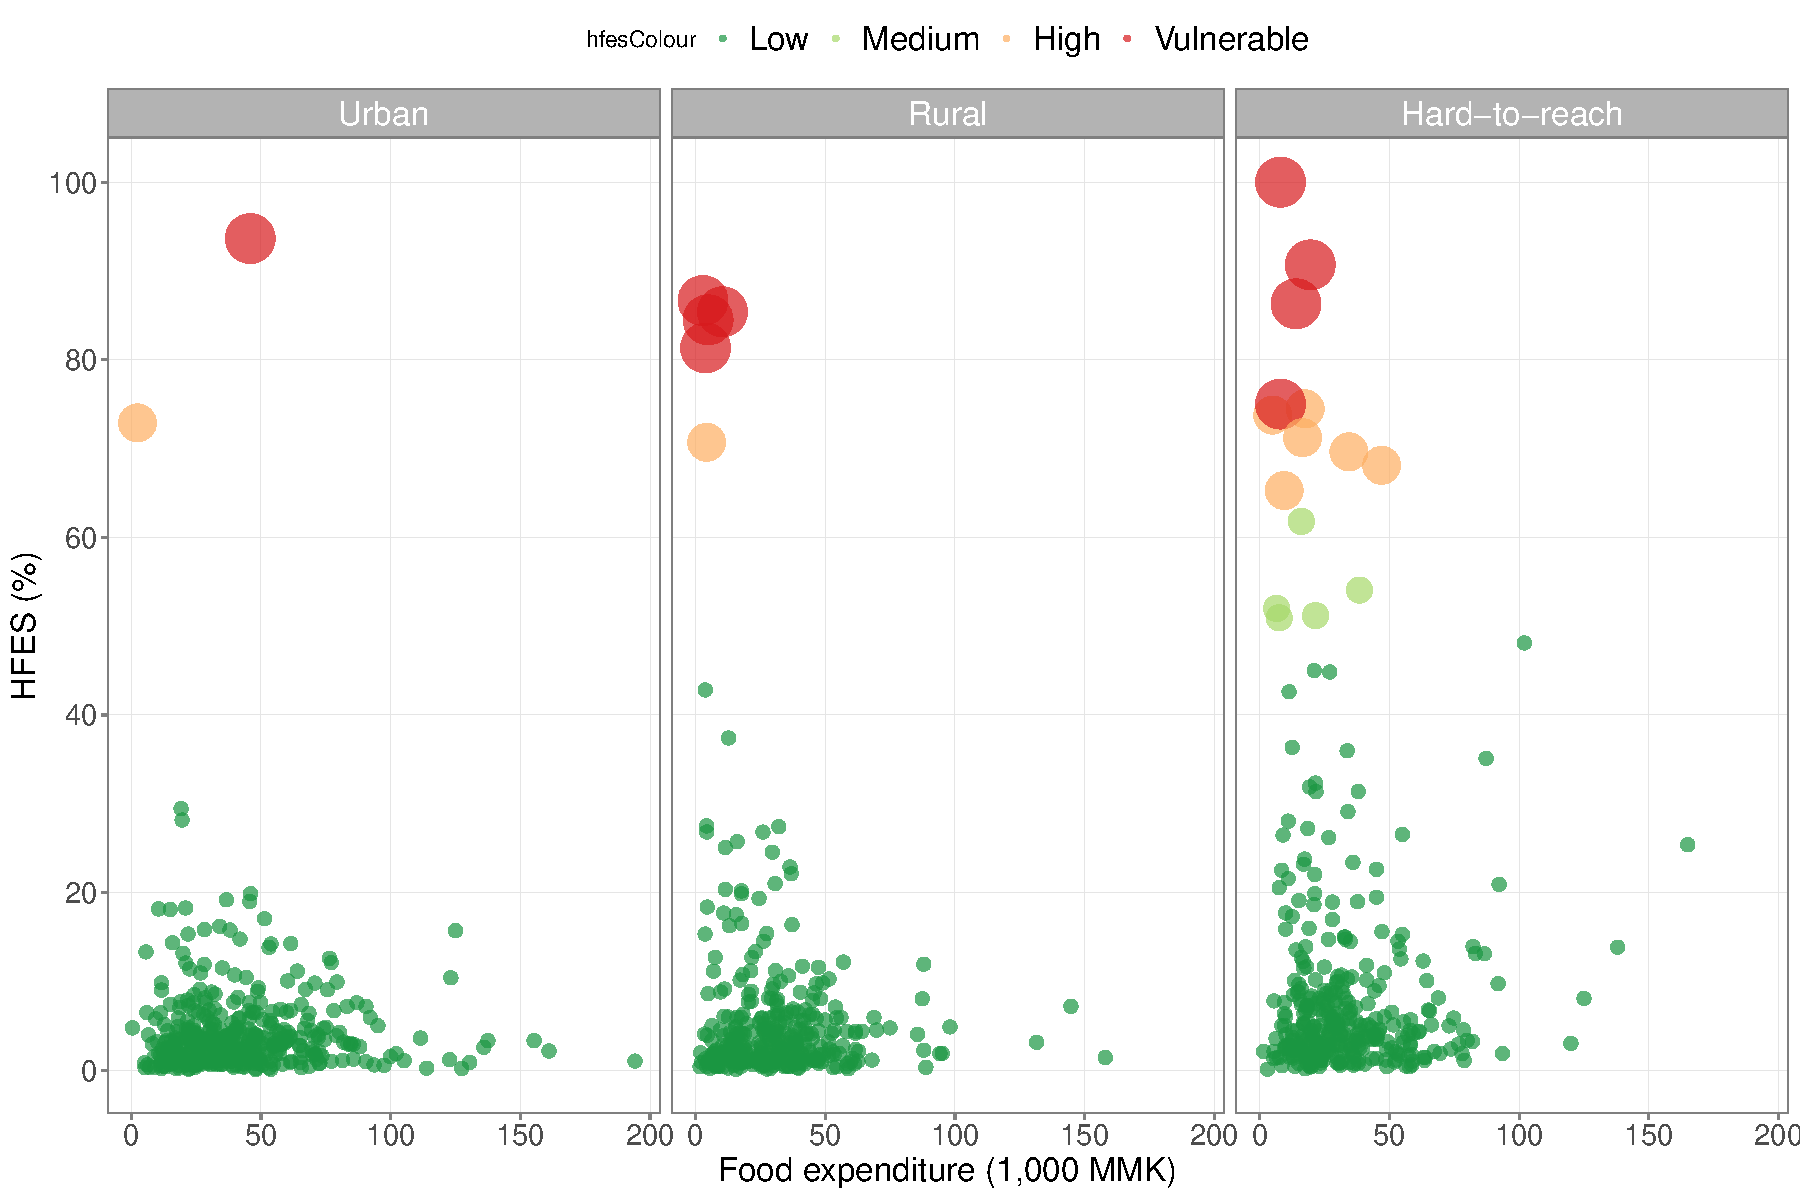
\includegraphics{kayinReport_files/figure-latex/hfesScatterPlot1-1} 

}

\caption{Household food expenditure share by location type}\label{fig:hfesScatterPlot1}
\end{figure}

\begin{figure}[H]

{\centering 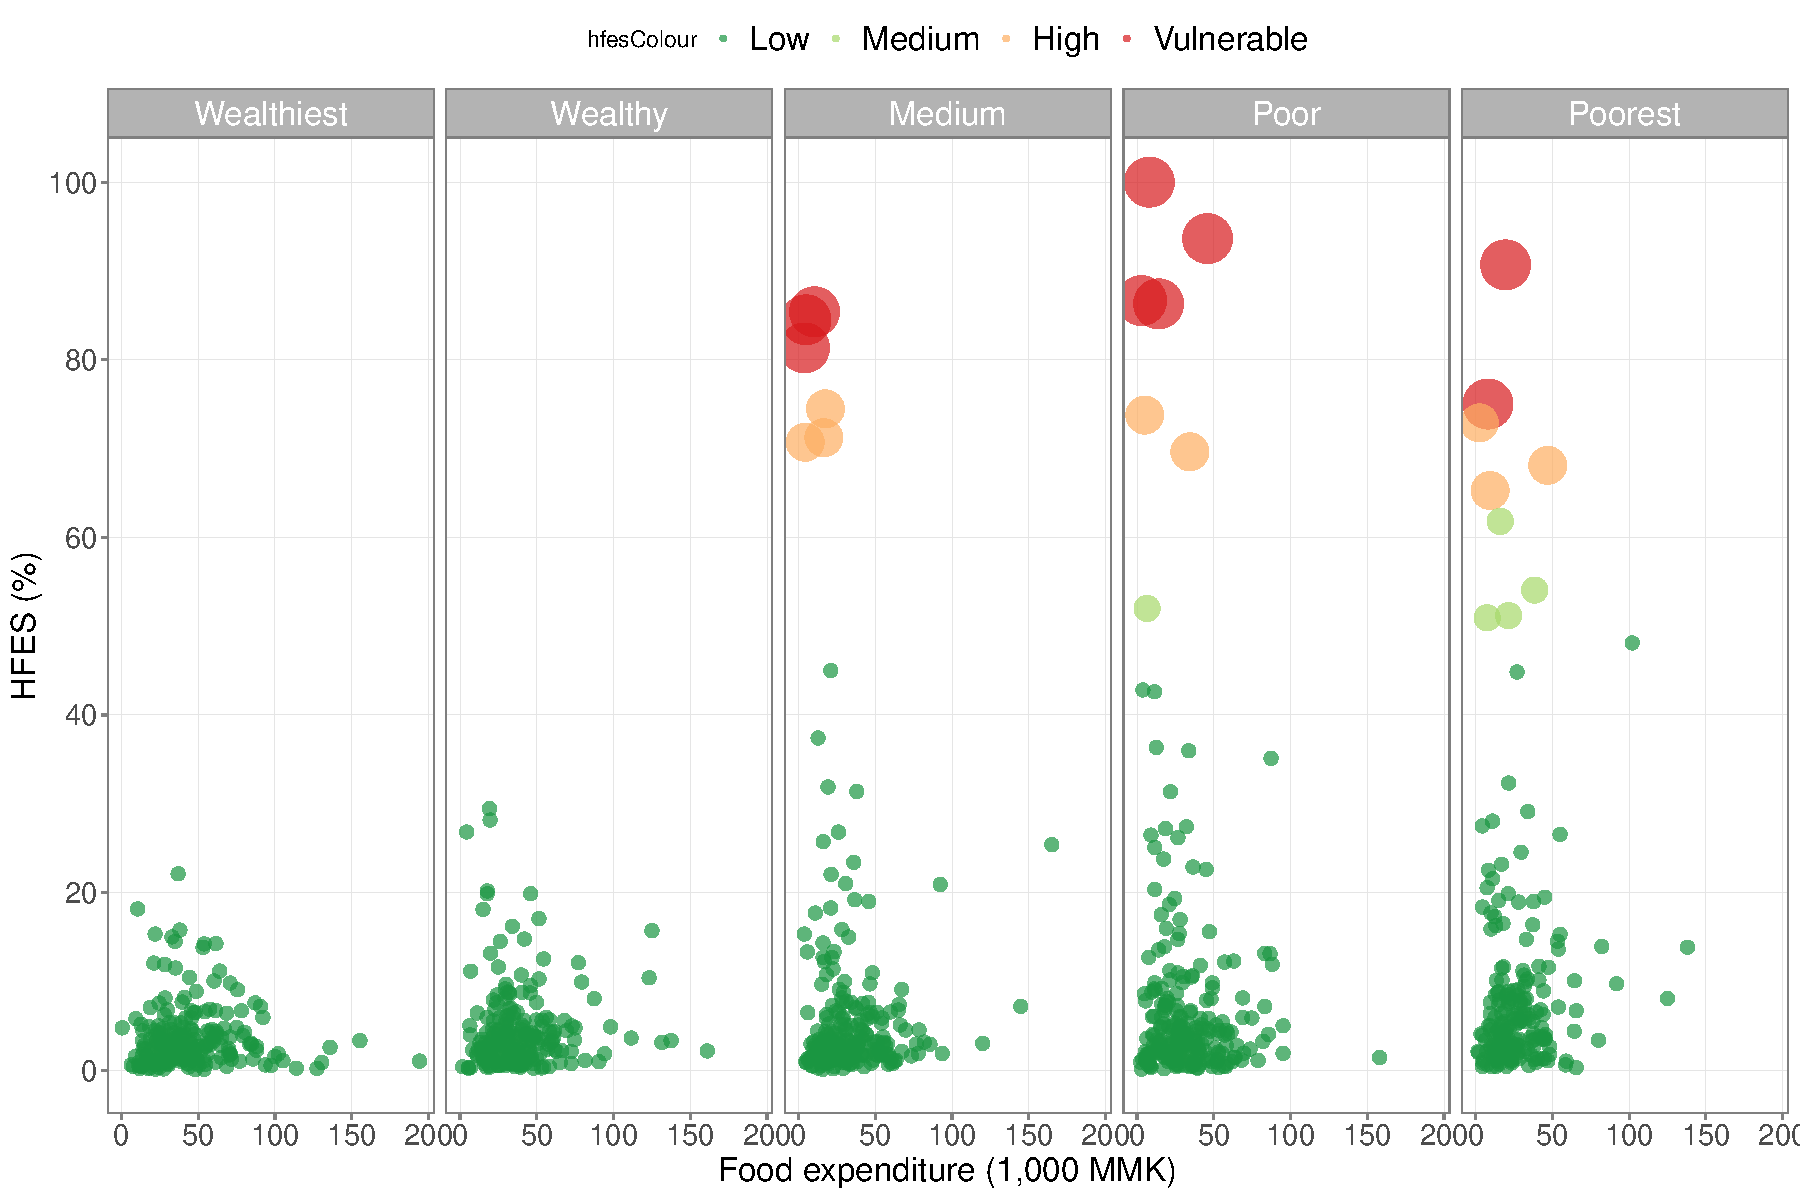
\includegraphics{kayinReport_files/figure-latex/hfesScatterPlot2-1} 

}

\caption{Household food expenditure share by wealth quintiles}\label{fig:hfesScatterPlot2}
\end{figure}

\hypertarget{wash-results}{%
\subsubsection{Water, sanitation and hygiene}\label{wash-results}}

\hypertarget{water-results}{%
\paragraph{Water services ladder}\label{water-results}}

There is minimal seasonal variation in households' access to drinking water with a majority of households able to get water from improved sources of drinking water whole year round (see \ref{tab:wash1table}). However, up to 18\% of households in hard-to-reach areas use surface water as their drinking water source (see Figure \ref{fig:wash1plot}). Interestingly, in urban areas, up to 4\% still access drinking water from surface water. Figure \ref{fig:wash2plot} show that the poorer the household gets, the higher the probability that the household is accessing drinking water from surface water.

\begin{table}[H]

\caption{\label{tab:wash1table}Water service ladders}
\centering
\fontsize{8}{10}\selectfont
\begin{tabular}[t]{>{\bfseries}l>{\bfseries}l>{\ttfamily}r>{\ttfamily}r>{\ttfamily}r>{\ttfamily}r>{\ttfamily}r>{\ttfamily}r>{\ttfamily}r>{\ttfamily}r>{\ttfamily}r}
\toprule
\multicolumn{2}{c}{\textbf{ }} & \multicolumn{3}{c}{\textbf{Summer Season}} & \multicolumn{3}{c}{\textbf{Rainy Season}} & \multicolumn{3}{c}{\textbf{Winter Season}} \\
\cmidrule(l{3pt}r{3pt}){3-5} \cmidrule(l{3pt}r{3pt}){6-8} \cmidrule(l{3pt}r{3pt}){9-11}
 &  & \makecell[c]{At least\\limited\\(\%)} & \makecell[c]{Unimproved\\(\%)} & \makecell[c]{Surface\\water\\(\%)} & \makecell[c]{At least\\limited\\(\%)} & \makecell[c]{Unimproved\\(\%)} & \makecell[c]{Surface\\water\\(\%)} & \makecell[c]{At least\\limited\\(\%)} & \makecell[c]{Unimproved\\(\%)} & \makecell[c]{Surface\\water\\(\%)}\\
\midrule
\addlinespace[0.3em]
\multicolumn{11}{l}{\textbf{Kayin}}\\
\addlinespace[0.3em]
\multicolumn{11}{l}{\textit{\textbf{Geographic}}}\\
\hspace{1em}\hspace{1em} & Rural & 90.8 & 5.2 & 4.0 & 91.0 & 5.8 & 3.2 & 91.0 & 5.2 & 3.8\\
\cmidrule{2-11}
\hspace{1em}\hspace{1em} & Urban & 95.8 & 3.5 & 0.7 & 96.3 & 3.5 & 0.2 & 96.0 & 3.5 & 0.5\\
\cmidrule{2-11}
\hspace{1em}\hspace{1em} & Hard-to-reach & 57.7 & 18.0 & 24.3 & 65.1 & 15.1 & 19.7 & 60.0 & 16.9 & 23.1\\
\cmidrule{2-11}
\addlinespace[0.3em]
\multicolumn{11}{l}{\textit{\textbf{Wealth}}}\\
\hspace{1em}\hspace{1em} & Wealthiest & 97.6 & 1.9 & 0.5 & 98.6 & 1.4 & 0.0 & 97.1 & 2.4 & 0.5\\
\cmidrule{2-11}
\hspace{1em}\hspace{1em} & Wealthy & 91.3 & 4.3 & 4.3 & 93.5 & 4.3 & 2.2 & 91.8 & 3.9 & 4.3\\
\cmidrule{2-11}
\hspace{1em}\hspace{1em} & Medium & 77.3 & 11.1 & 11.6 & 80.6 & 9.3 & 10.2 & 78.2 & 10.6 & 11.1\\
\cmidrule{2-11}
\hspace{1em}\hspace{1em} & Poor & 71.5 & 14.9 & 13.6 & 76.0 & 13.1 & 10.9 & 72.9 & 14.5 & 12.7\\
\cmidrule{2-11}
\hspace{1em}\hspace{1em} & Poorest & 72.6 & 11.2 & 16.1 & 74.9 & 11.7 & 13.5 & 74.9 & 10.3 & 14.8\\
\bottomrule
\end{tabular}
\end{table}

\newpage

\begin{figure}[H]

{\centering 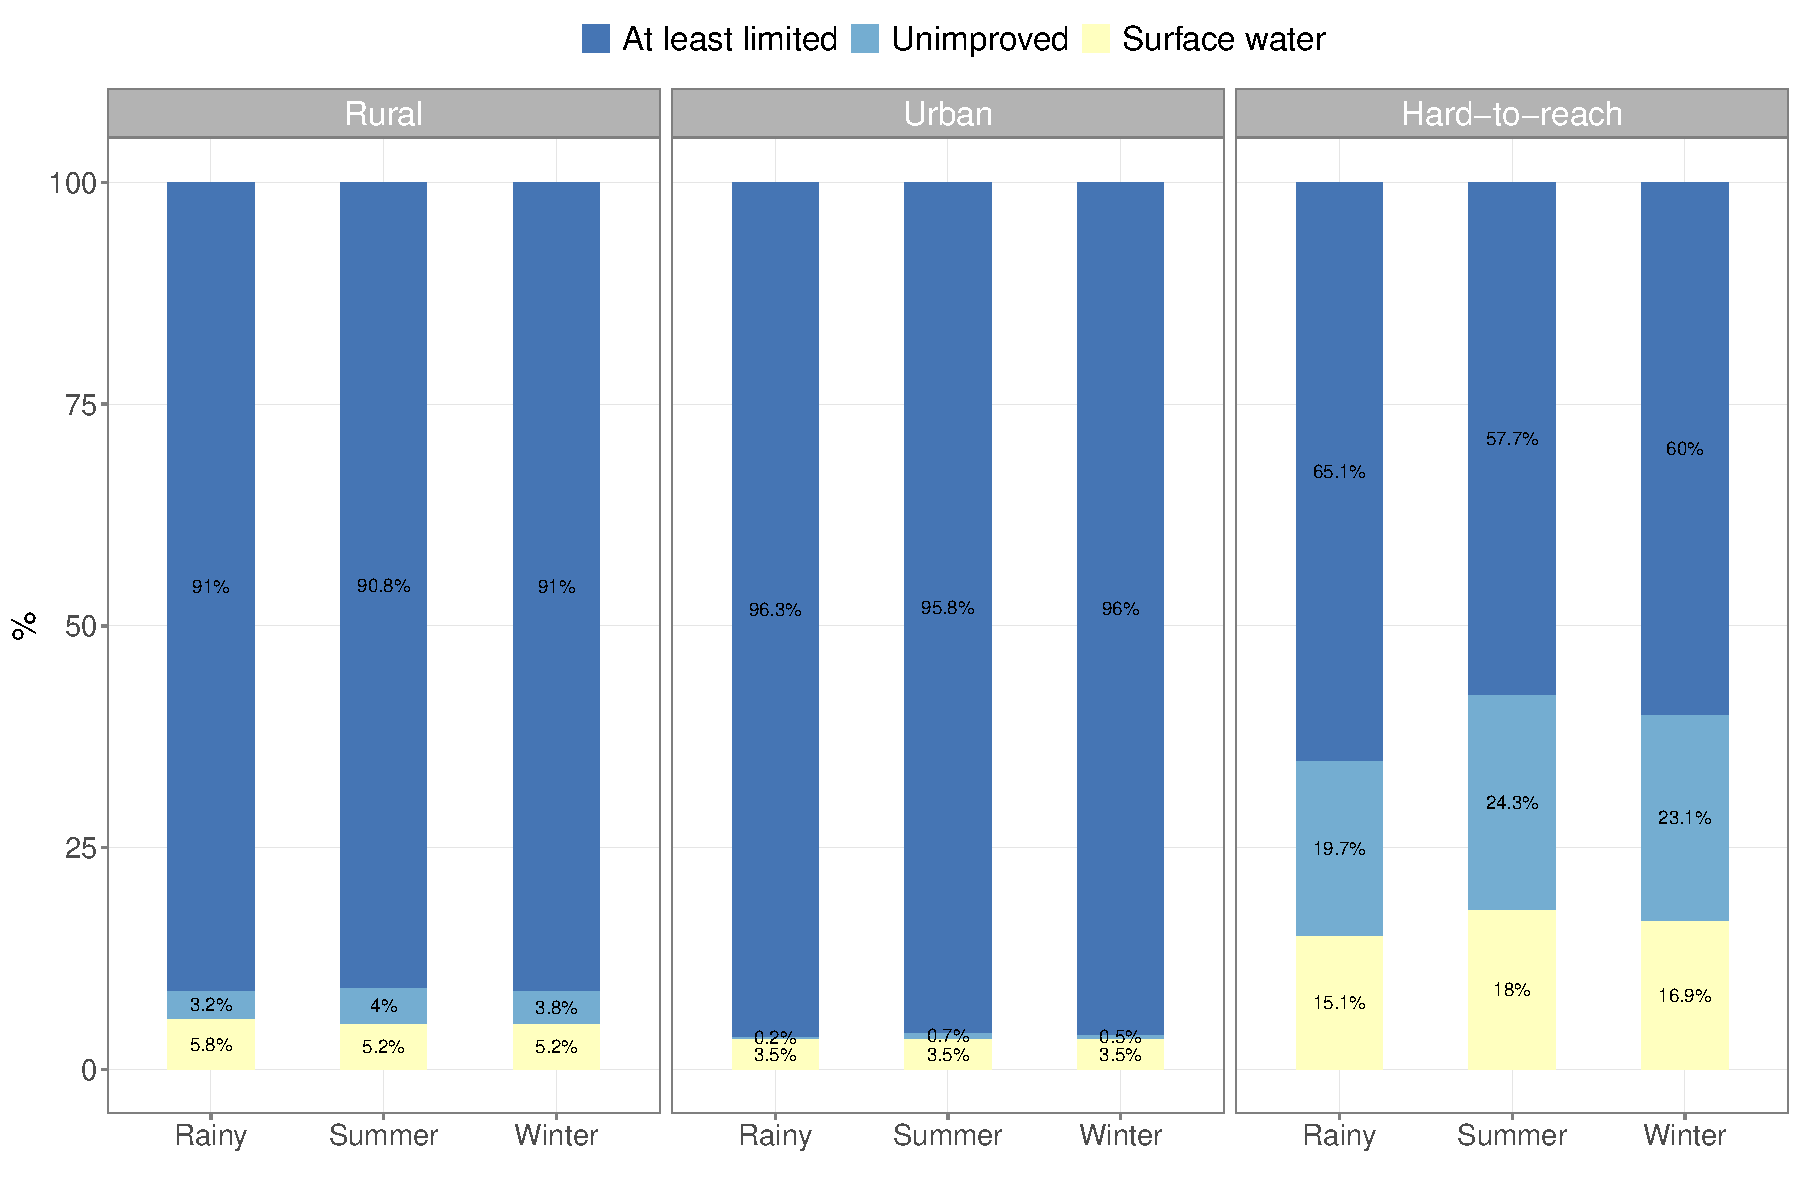
\includegraphics{kayinReport_files/figure-latex/wash1plot-1} 

}

\caption{Water services ladder by location type}\label{fig:wash1plot}
\end{figure}

\begin{figure}[H]

{\centering 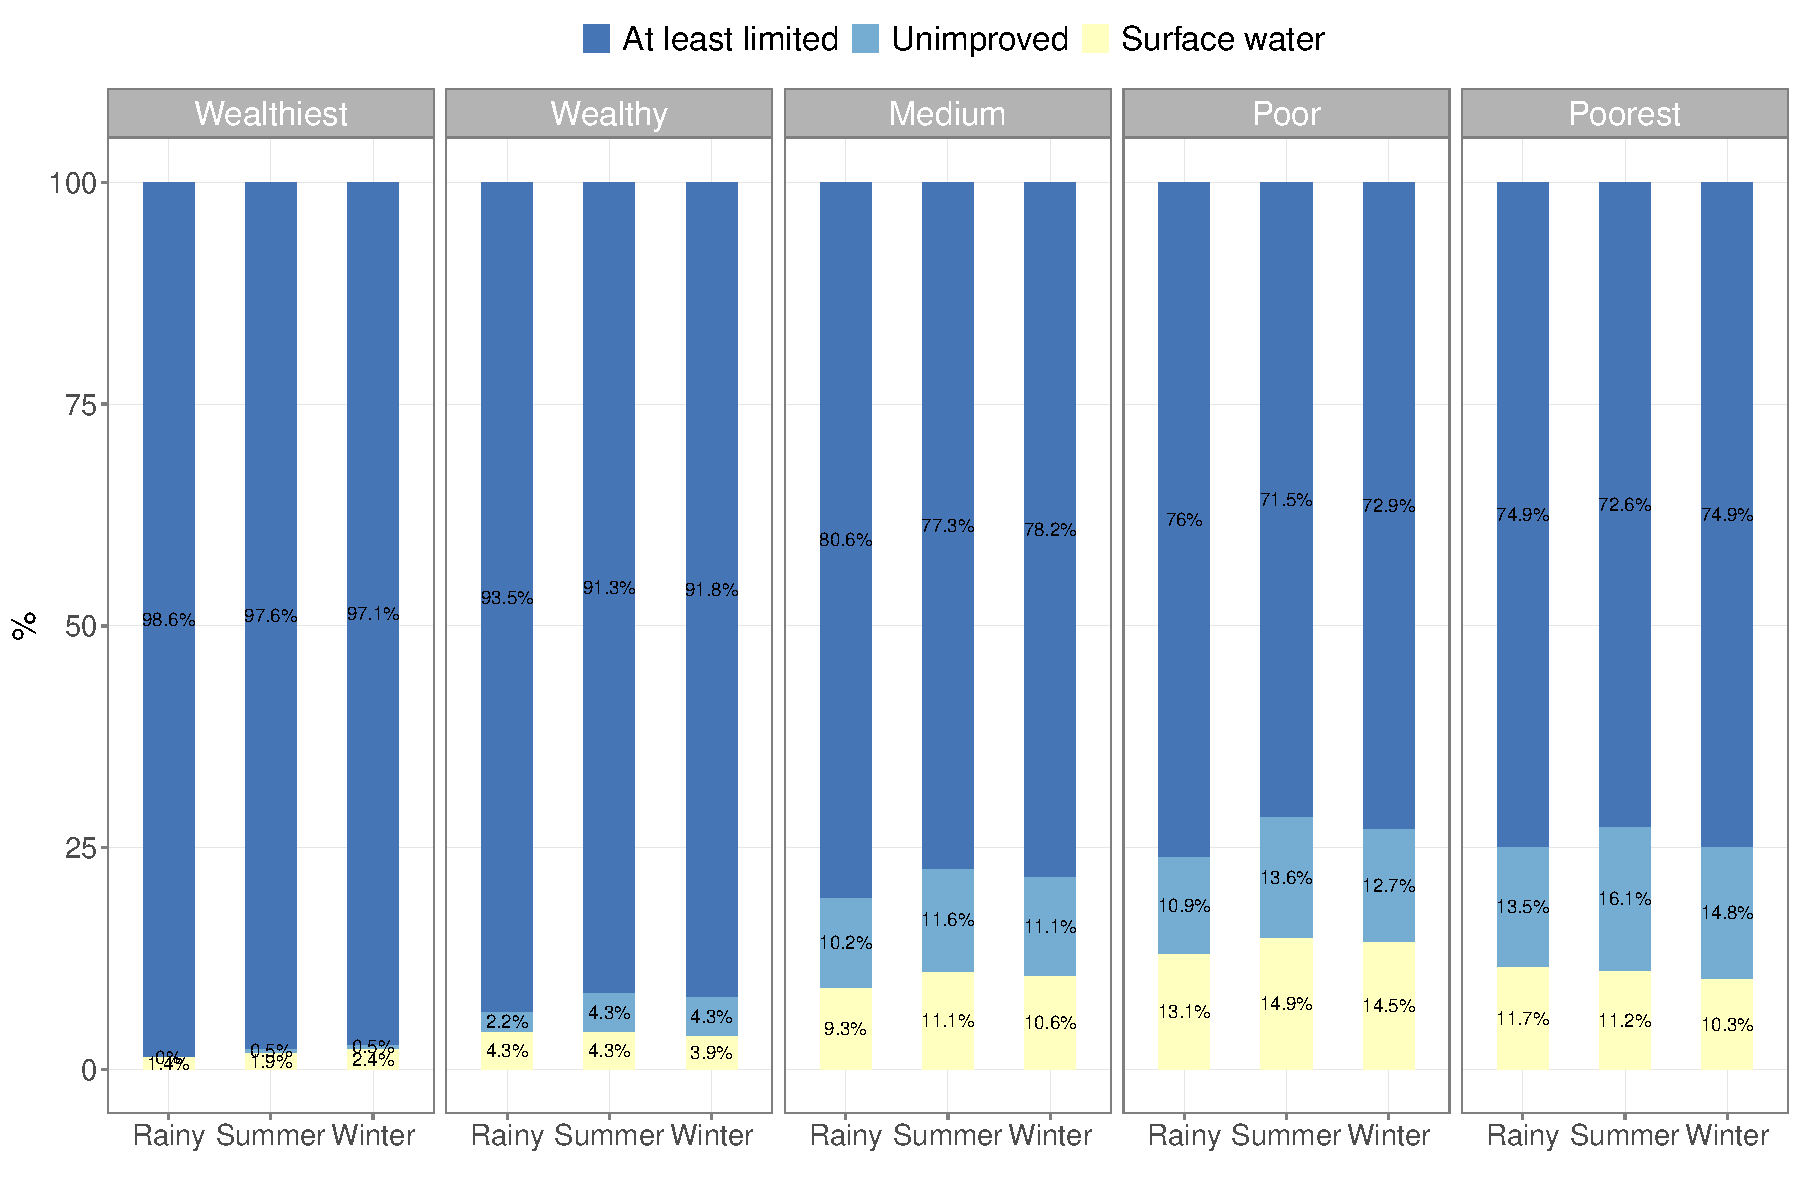
\includegraphics{kayinReport_files/figure-latex/wash2plot-1} 

}

\caption{Water services ladder by wealth quintiles}\label{fig:wash2plot}
\end{figure}

\hypertarget{sanitation-services-ladder}{%
\paragraph{Sanitation services ladder}\label{sanitation-services-ladder}}

Up to 78\% of households in urban areas of Kayin state have at least limited (improved toilet facility but shared with other households) or basic (improved sanitation facility and not shared with other households) sanitation facilities (see Table \ref{tab:san1table}). On the other hand, unimproved sanitation facilities and open defection are used by more households in hard-to-reach areas (see \ref{fig:san1plot}) and increasingly used as households get poorer (see Figure \ref{fig:san2plot}). Up to 7.7\% of wealthiest households and 19\% of wealthy households have unimproved sanitation facilities.

\begin{table}[H]

\caption{\label{tab:san1table}Sanitation service ladders}
\centering
\fontsize{12}{14}\selectfont
\begin{tabular}[t]{>{\bfseries}l>{\bfseries}l>{\ttfamily}r>{\ttfamily}r>{\ttfamily}r>{\ttfamily}r}
\toprule
 &  & \makecell[c]{Basic\\(\%)} & \makecell[c]{Limited\\(\%)} & \makecell[c]{Unimproved\\(\%)} & \makecell[c]{Open\\Defecation\\(\%)}\\
\midrule
\addlinespace[0.3em]
\multicolumn{6}{l}{\textbf{Kayin}}\\
\addlinespace[0.3em]
\multicolumn{6}{l}{\textit{\textbf{Geographic}}}\\
\hspace{1em}\hspace{1em} & Rural & 12.4 & 49.1 & 25.4 & 11.6\\
\cmidrule{2-6}
\hspace{1em}\hspace{1em} & Urban & 14.8 & 63.2 & 20.4 & 0.2\\
\cmidrule{2-6}
\hspace{1em}\hspace{1em} & Hard-to-reach & 16.9 & 32.3 & 14.9 & 36.0\\
\cmidrule{2-6}
\addlinespace[0.3em]
\multicolumn{6}{l}{\textit{\textbf{Wealth}}}\\
\hspace{1em}\hspace{1em} & Wealthiest & 14.4 & 77.5 & 7.7 & 0.0\\
\cmidrule{2-6}
\hspace{1em}\hspace{1em} & Wealthy & 14.3 & 63.2 & 19.0 & 2.6\\
\cmidrule{2-6}
\hspace{1em}\hspace{1em} & Medium & 17.6 & 42.1 & 29.2 & 10.2\\
\cmidrule{2-6}
\hspace{1em}\hspace{1em} & Poor & 12.2 & 37.1 & 26.7 & 22.6\\
\cmidrule{2-6}
\hspace{1em}\hspace{1em} & Poorest & 14.3 & 25.1 & 19.3 & 39.9\\
\bottomrule
\end{tabular}
\end{table}

\newpage

\begin{figure}[H]

{\centering 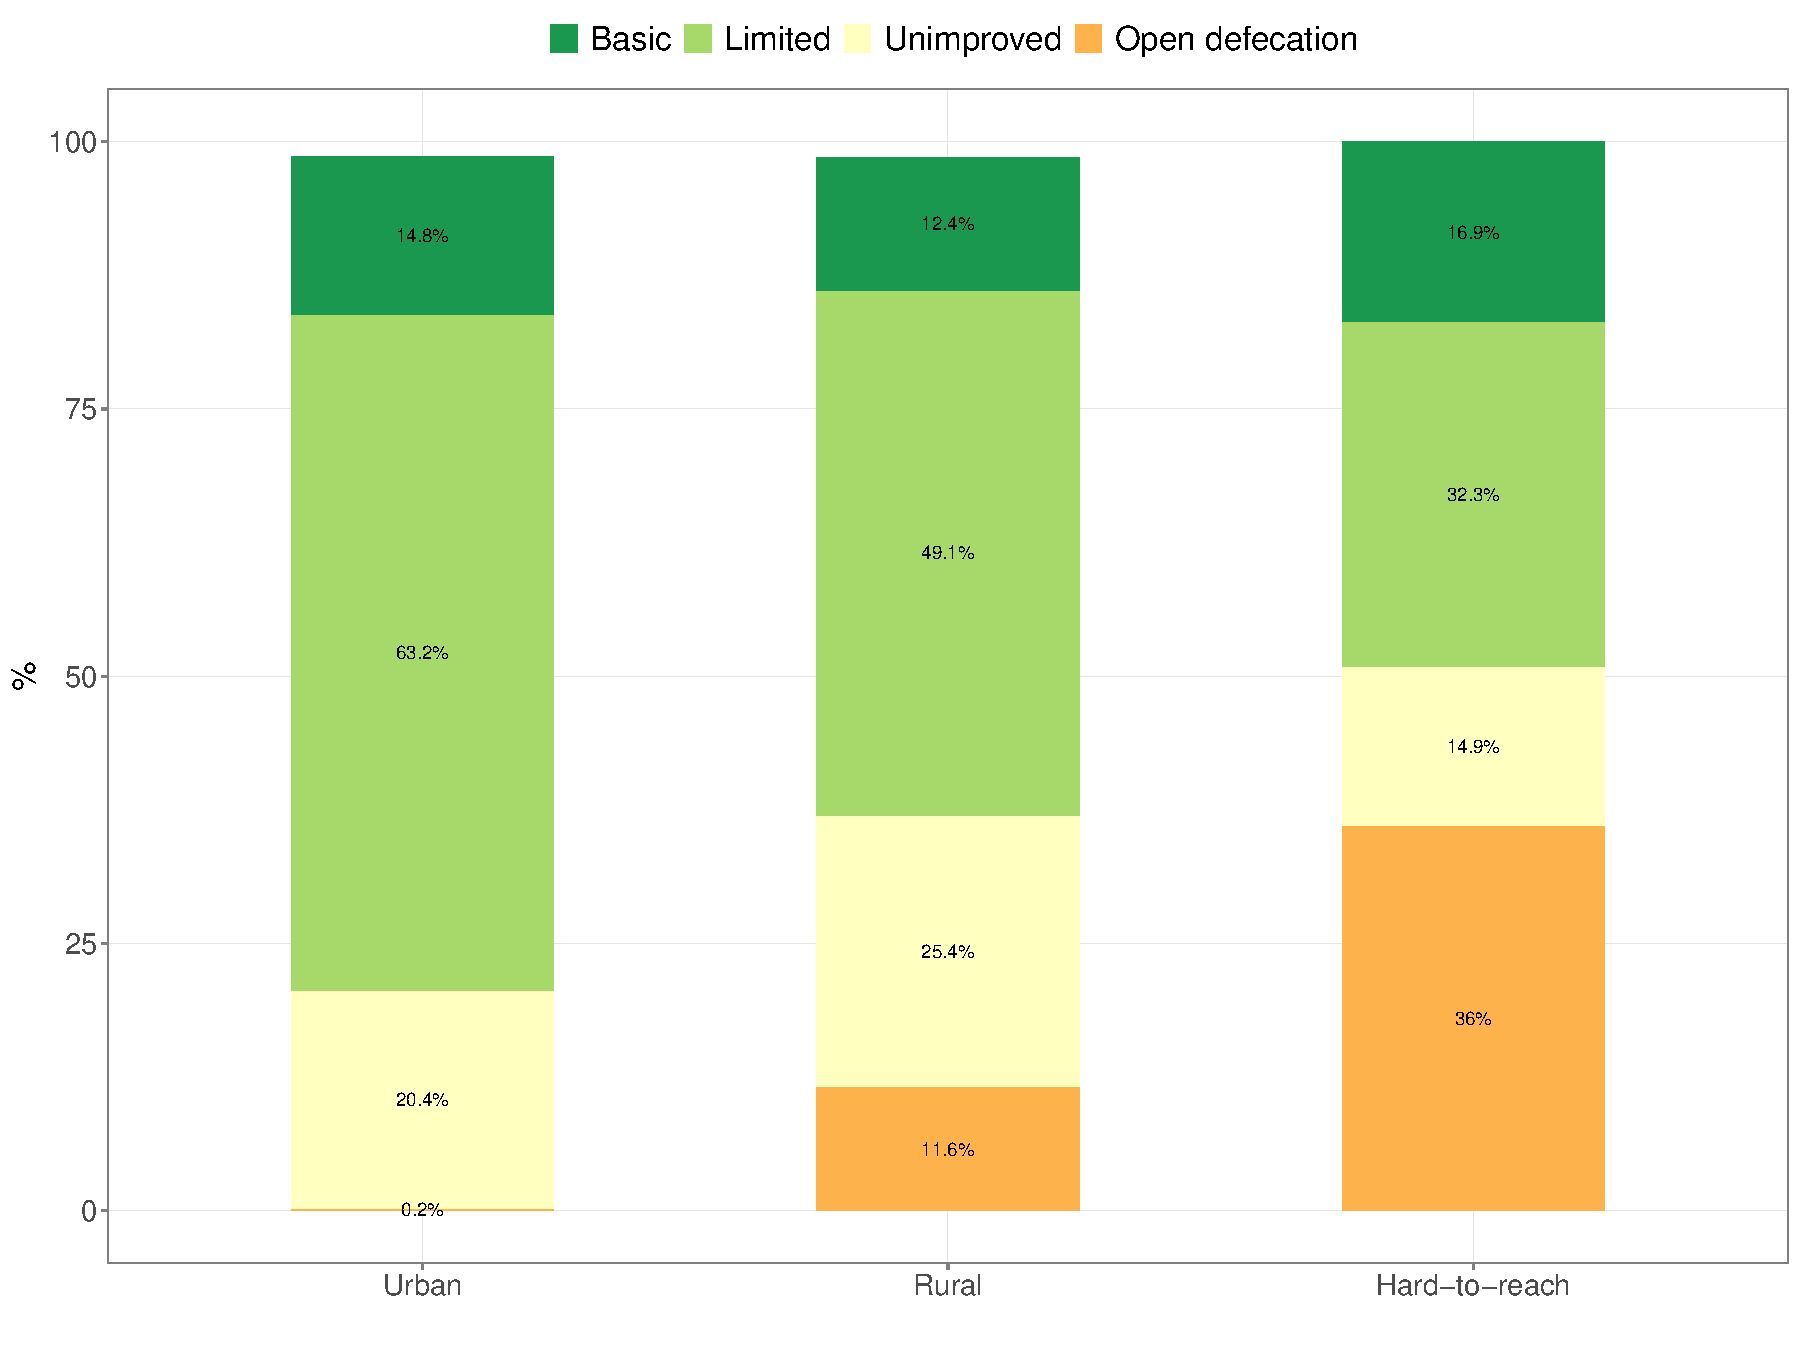
\includegraphics{kayinReport_files/figure-latex/san1plot-1} 

}

\caption{Sanitation services ladder by location type}\label{fig:san1plot}
\end{figure}

\begin{figure}[H]

{\centering 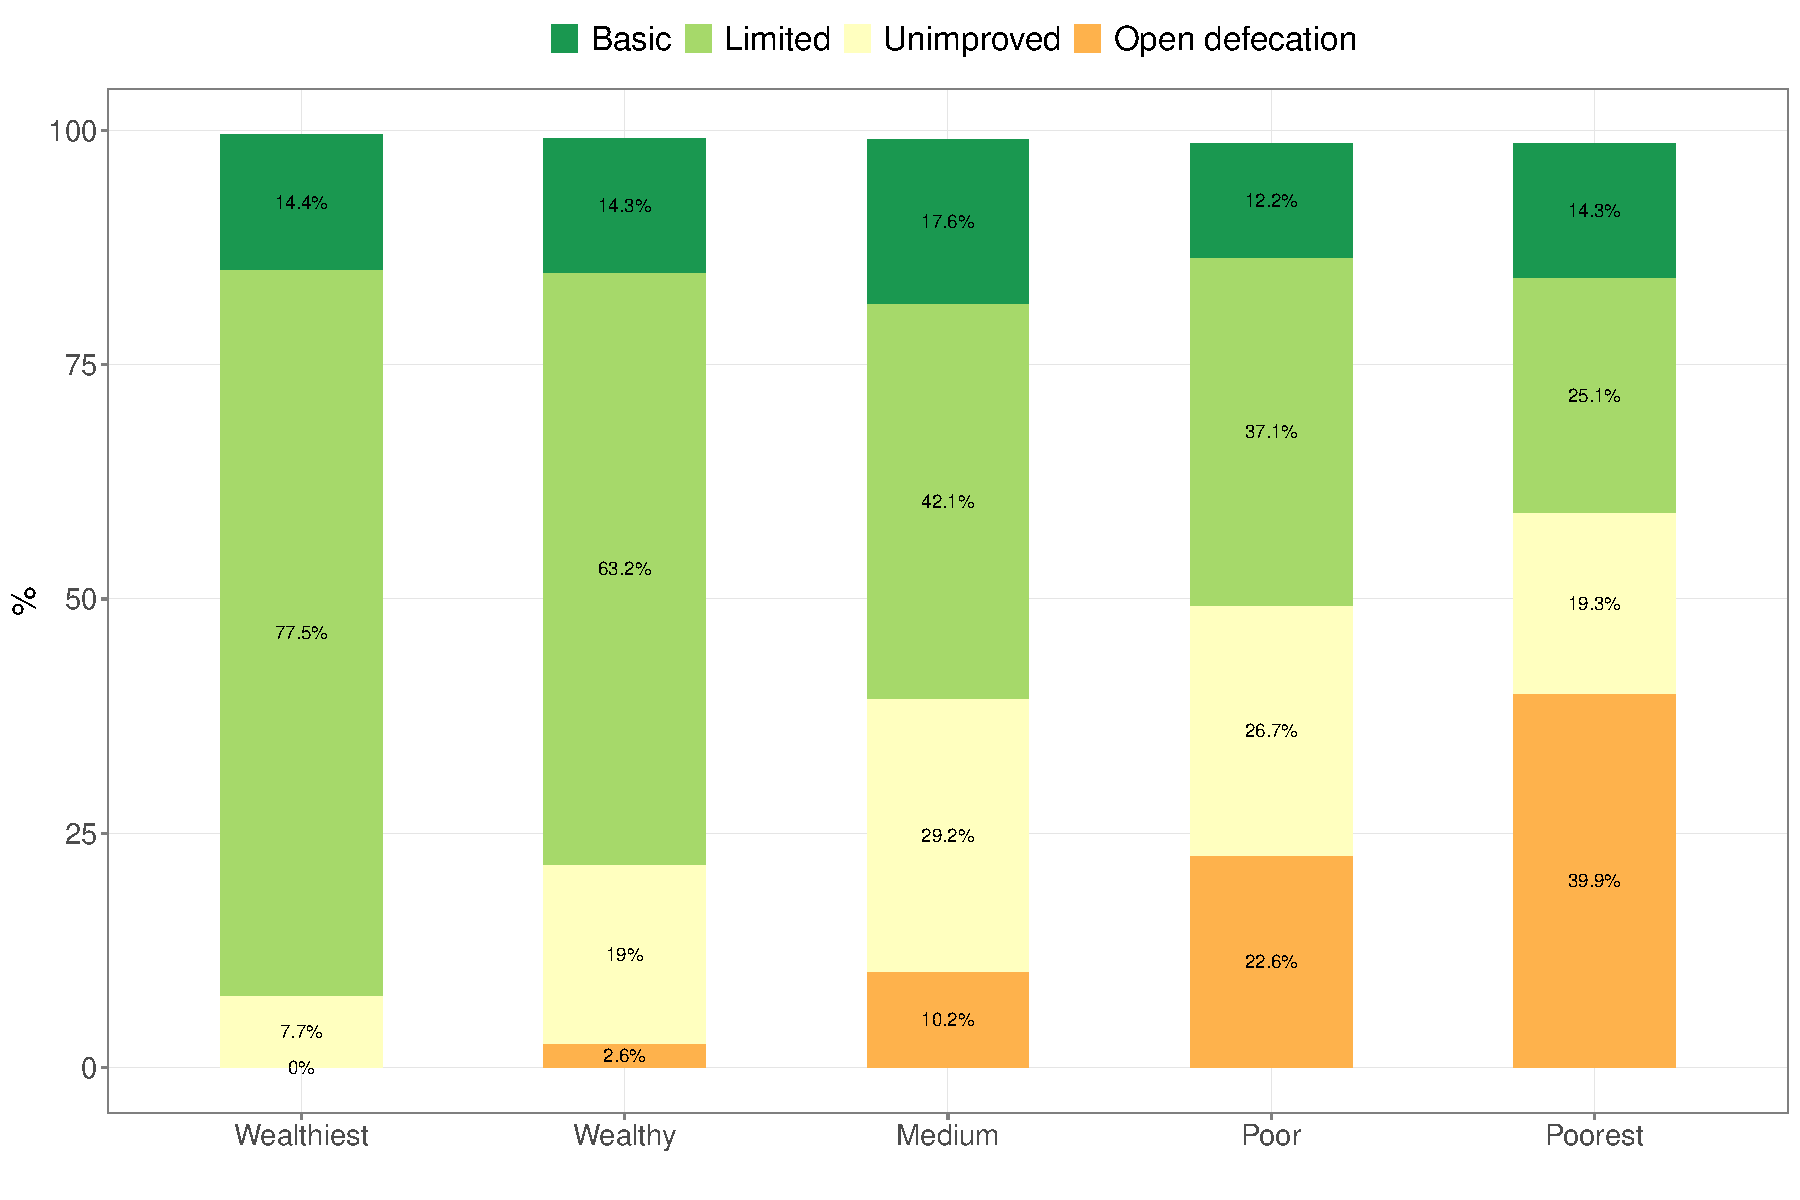
\includegraphics{kayinReport_files/figure-latex/san2plot-1} 

}

\caption{Water services ladder by wealth quintiles}\label{fig:san2plot}
\end{figure}

\hypertarget{handwashing-service-ladder}{%
\paragraph{Handwashing service ladder}\label{handwashing-service-ladder}}

Access to basic (handwashing facilities with water and soap) handwashing facilities is as high as 93.8\% in urban areas and 87.9\% in rural areas. Hard-to-reach areas on the other hand have much lower access to basic facilities and with the highest proportion of households with no facilities at all (see Figure \ref{fig:handwashing1plot}). The same trend exists as households get poorer with the poorest households having low levels of access to basic handwashing facilities and highest levels of no handwashing facilities (see Figure \ref{fig:handwashing2plot}).

\begin{table}[H]

\caption{\label{tab:handwashing1table}Handwashing service ladders}
\centering
\fontsize{12}{14}\selectfont
\begin{tabular}[t]{>{\bfseries}l>{\bfseries}l>{\ttfamily}r>{\ttfamily}r>{\ttfamily}r}
\toprule
 &  & \makecell[c]{Basic\\(\%)} & \makecell[c]{Limited\\(\%)} & \makecell[c]{No\\Facility\\(\%)}\\
\midrule
\addlinespace[0.3em]
\multicolumn{5}{l}{\textbf{Kayin}}\\
\addlinespace[0.3em]
\multicolumn{5}{l}{\textit{\textbf{Geographic}}}\\
\hspace{1em}\hspace{1em} & Rural & 87.9 & 0.3 & 3.5\\
\cmidrule{2-5}
\hspace{1em}\hspace{1em} & Urban & 93.8 & 0.0 & 2.1\\
\cmidrule{2-5}
\hspace{1em}\hspace{1em} & Hard-to-reach & 46.0 & 2.3 & 6.9\\
\cmidrule{2-5}
\addlinespace[0.3em]
\multicolumn{5}{l}{\textit{\textbf{Wealth}}}\\
\hspace{1em}\hspace{1em} & Wealthiest & 96.2 & 0.0 & 0.5\\
\cmidrule{2-5}
\hspace{1em}\hspace{1em} & Wealthy & 88.7 & 0.0 & 3.5\\
\cmidrule{2-5}
\hspace{1em}\hspace{1em} & Medium & 79.6 & 0.5 & 4.6\\
\cmidrule{2-5}
\hspace{1em}\hspace{1em} & Poor & 67.4 & 0.9 & 6.8\\
\cmidrule{2-5}
\hspace{1em}\hspace{1em} & Poorest & 54.7 & 2.7 & 4.9\\
\bottomrule
\end{tabular}
\end{table}

\newpage

\begin{figure}[H]

{\centering 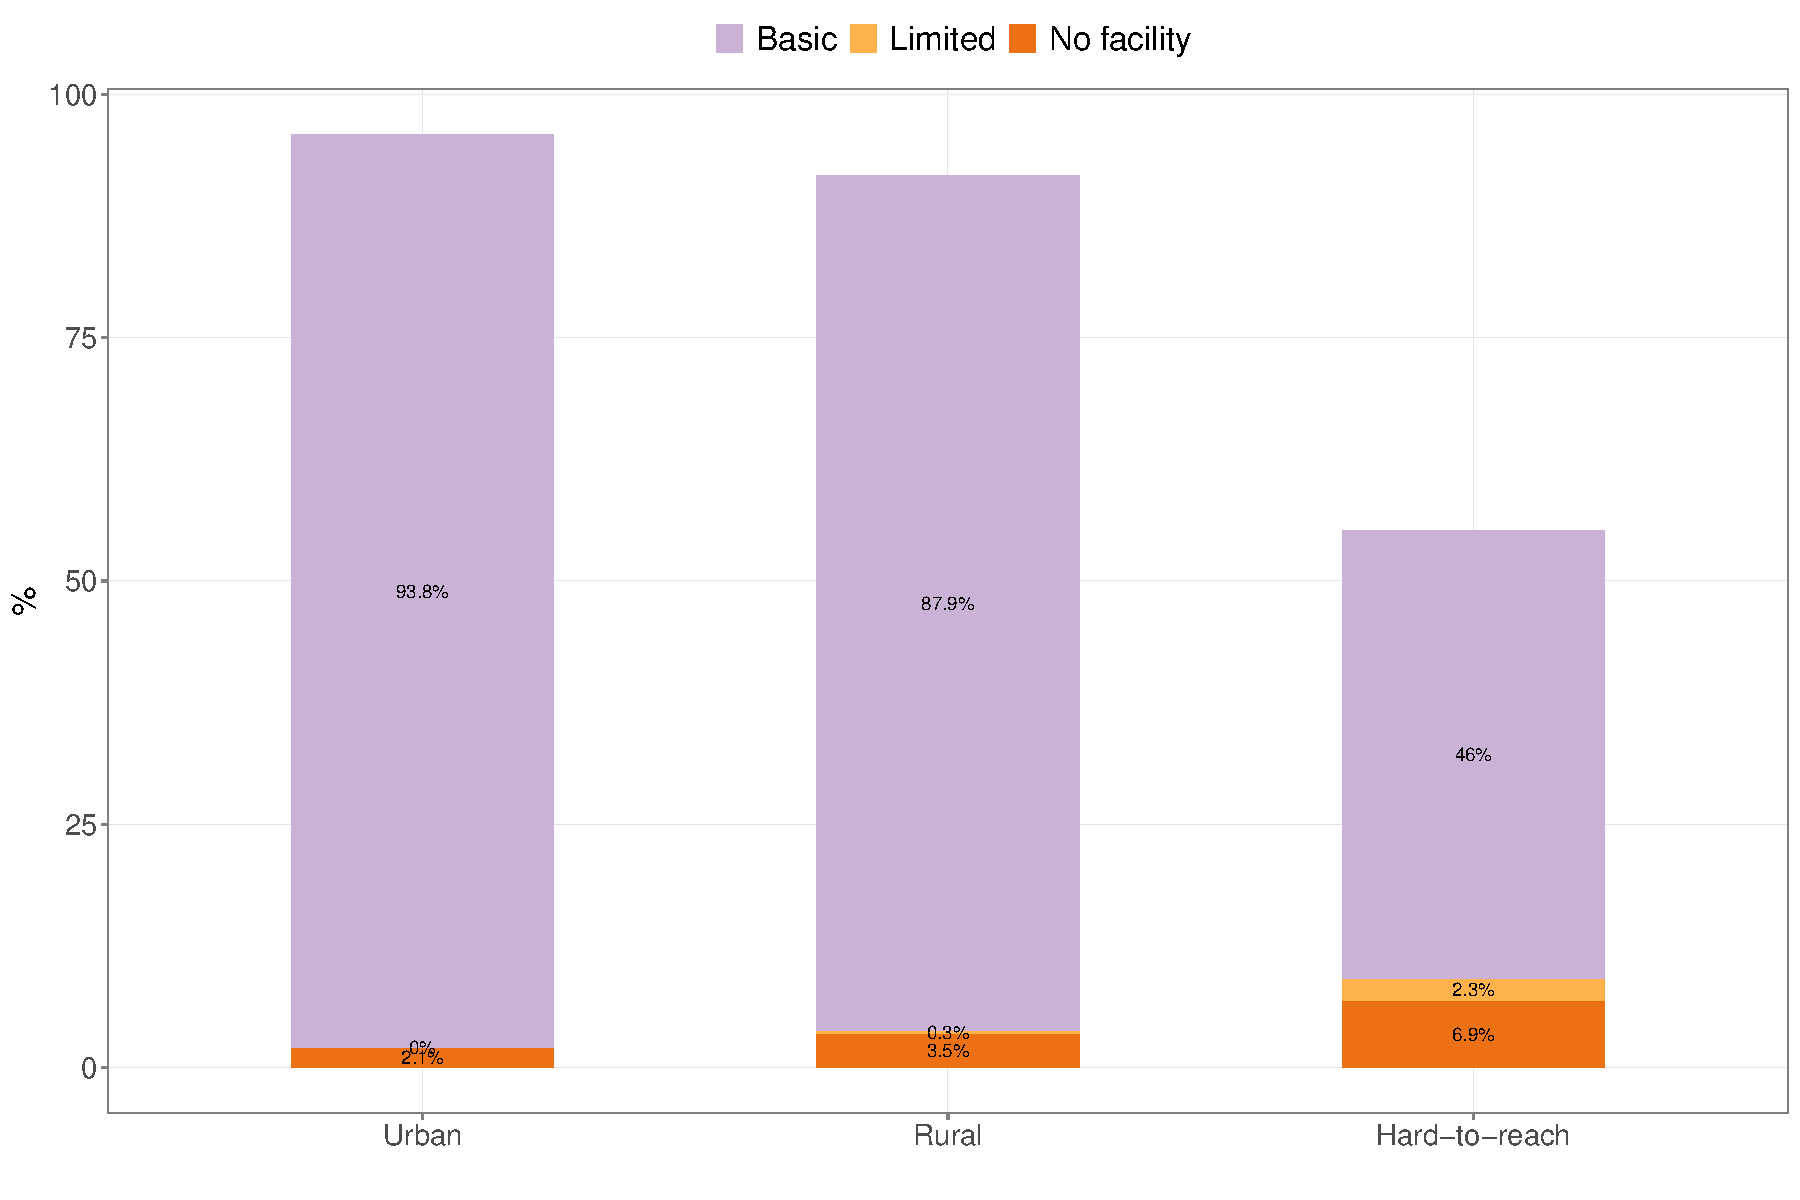
\includegraphics{kayinReport_files/figure-latex/handwashing1plot-1} 

}

\caption{Handwashing services ladder by location type}\label{fig:handwashing1plot}
\end{figure}

\begin{figure}[H]

{\centering 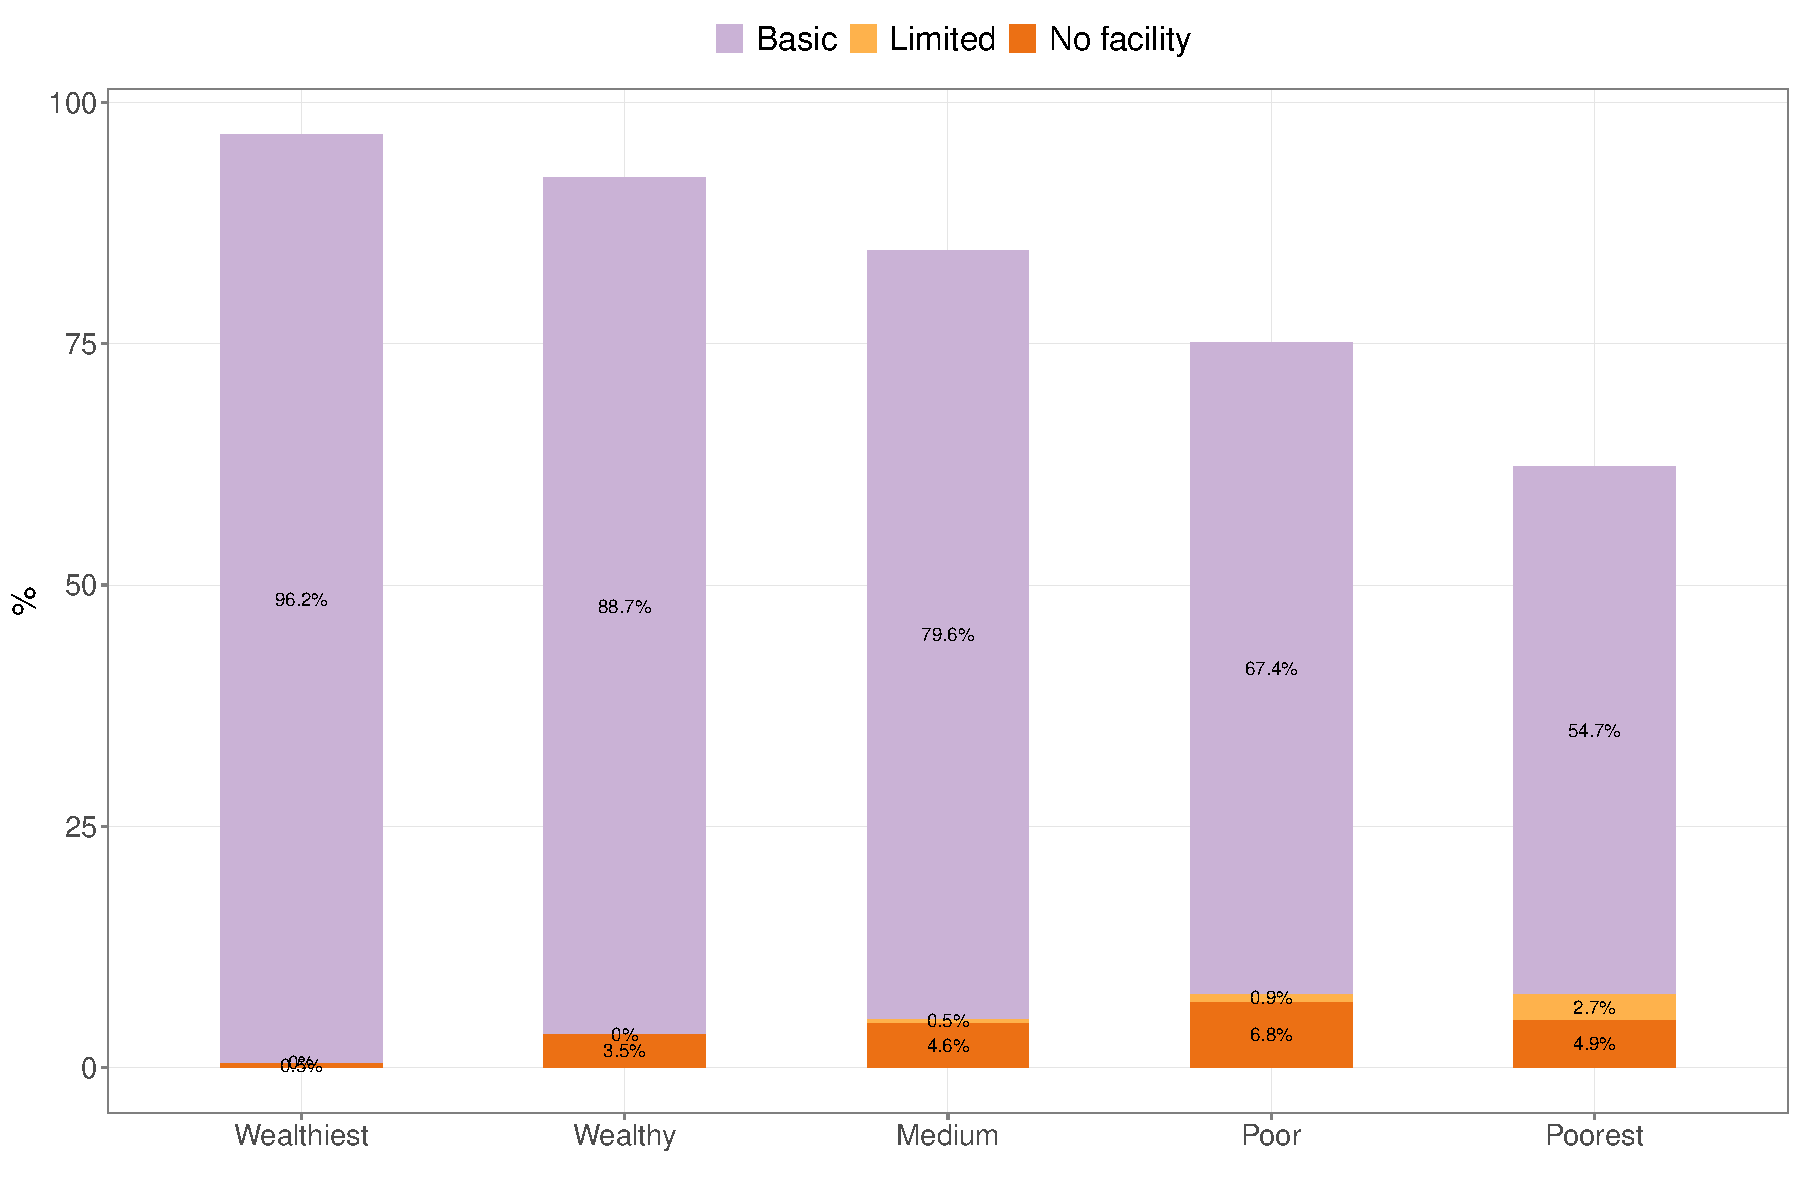
\includegraphics{kayinReport_files/figure-latex/handwashing2plot-1} 

}

\caption{Handwashing services ladder by wealth quintiles}\label{fig:handwashing2plot}
\end{figure}

\hypertarget{chealth-results}{%
\subsubsection{Child health}\label{chealth-results}}

\hypertarget{epi-results}{%
\paragraph{Immunisation coverage}\label{epi-results}}

Immunisation coverage in Kayin state tells a story of a generally wide exposure to immunisation services with nearly all children having had any immunisation in urban and rural areas and up to 86\% in hard-to-reach areas then falters early and dramatically with immunisation access as proxied by BCG vaccination drastically dropping to only as high as 22\% in urban and rural areas and 15\% in hard-to-reach areas. This drop in immunisation coverage continues with utilisation of immunisation services (as proxied by children getting all required pentavalent vaccinations) further drops particularly in hard-to-reach areas and then full immunisation coverage drops significantly in all areas but more profoundly in hard-to-reach areas (see Figure \ref{fig:epi1plot}).

Per vaccination type coverage, as to be expected, is significantly low across the whole of Kayin state (see Table \ref{tab:epi2table}) with households in hard-to-reach areas and poor and poorest households with significantly lower per vaccine type coverage, except for BCG, compared to urban and rural areas and wealthy and wealthiest households (see Figure \ref{fig:epi3plot} and Figure \ref{fig:epi4plot}).

Coverage of vitamin A supplementation, a service that is usually delivered together with immunisation, is relatively higher and going up to about 60\% in rural areas but much lower in urban and hard-to-reach areas (see Figure \ref{fig:epi5plot}) and lower in wealthiest and poorest households (see Figure \ref{fig:epi6plot}). Deworming coverage is low at only up to 25\% in rural areas and considerably lower in urban and hard-to-reach areas (see Figure \ref{fig:epi5plot}). Interestingly, poorest households have relatively higher deworming rates among wealth classes (see Figure \ref{fig:epi6plot}).

\begin{table}[H]

\caption{\label{tab:epi1table}Immunisation coverage}
\centering
\fontsize{8}{10}\selectfont
\begin{tabular}[t]{>{\bfseries}l>{\bfseries}l>{\ttfamily}r>{\ttfamily}r>{\ttfamily}r>{\ttfamily}r>{\ttfamily}r>{\ttfamily}r}
\toprule
 &  & \makecell[c]{Ever\\vaccinated\\(\%)} & \makecell[c]{Vaccination\\card\\retention\\rate\\(\%)} & \makecell[c]{Immunisation\\access\\(\%)} & \makecell[c]{Immunisation\\utilisation\\(\%)} & \makecell[c]{Full\\immunisation\\coverage\\(\%)} & \makecell[c]{Hepatitis B\\immunisation\\given\\within\\first\\24\\hours\\(\%)}\\
\midrule
\addlinespace[0.3em]
\multicolumn{8}{l}{\textbf{Kayin}}\\
\addlinespace[0.3em]
\multicolumn{8}{l}{\textit{\textbf{Geographic}}}\\
\hspace{1em}\hspace{1em} & Rural & 100.0 & 80.4 & 21.1 & 19.6 & 5.5 & 40.7\\
\cmidrule{2-8}
\hspace{1em}\hspace{1em} & Urban & 98.3 & 82.2 & 21.5 & 19.4 & 6.0 & 55.5\\
\cmidrule{2-8}
\hspace{1em}\hspace{1em} & Hard-to-reach & 85.5 & 75.4 & 15.2 & 10.3 & 3.7 & 25.0\\
\cmidrule{2-8}
\addlinespace[0.3em]
\multicolumn{8}{l}{\textit{\textbf{Wealth}}}\\
\hspace{1em}\hspace{1em} & Wealthiest & 100.0 & 90.7 & 19.8 & 18.3 & 4.6 & 57.5\\
\cmidrule{2-8}
\hspace{1em}\hspace{1em} & Wealthy & 100.0 & 76.1 & 23.1 & 20.0 & 6.6 & 51.9\\
\cmidrule{2-8}
\hspace{1em}\hspace{1em} & Medium & 96.9 & 85.7 & 21.2 & 18.4 & 4.5 & 41.0\\
\cmidrule{2-8}
\hspace{1em}\hspace{1em} & Poor & 94.2 & 81.6 & 16.7 & 14.0 & 6.2 & 36.4\\
\cmidrule{2-8}
\hspace{1em}\hspace{1em} & Poorest & 86.3 & 63.6 & 16.5 & 12.6 & 3.8 & 18.7\\
\bottomrule
\end{tabular}
\end{table}

\newpage

\begin{figure}[H]

{\centering 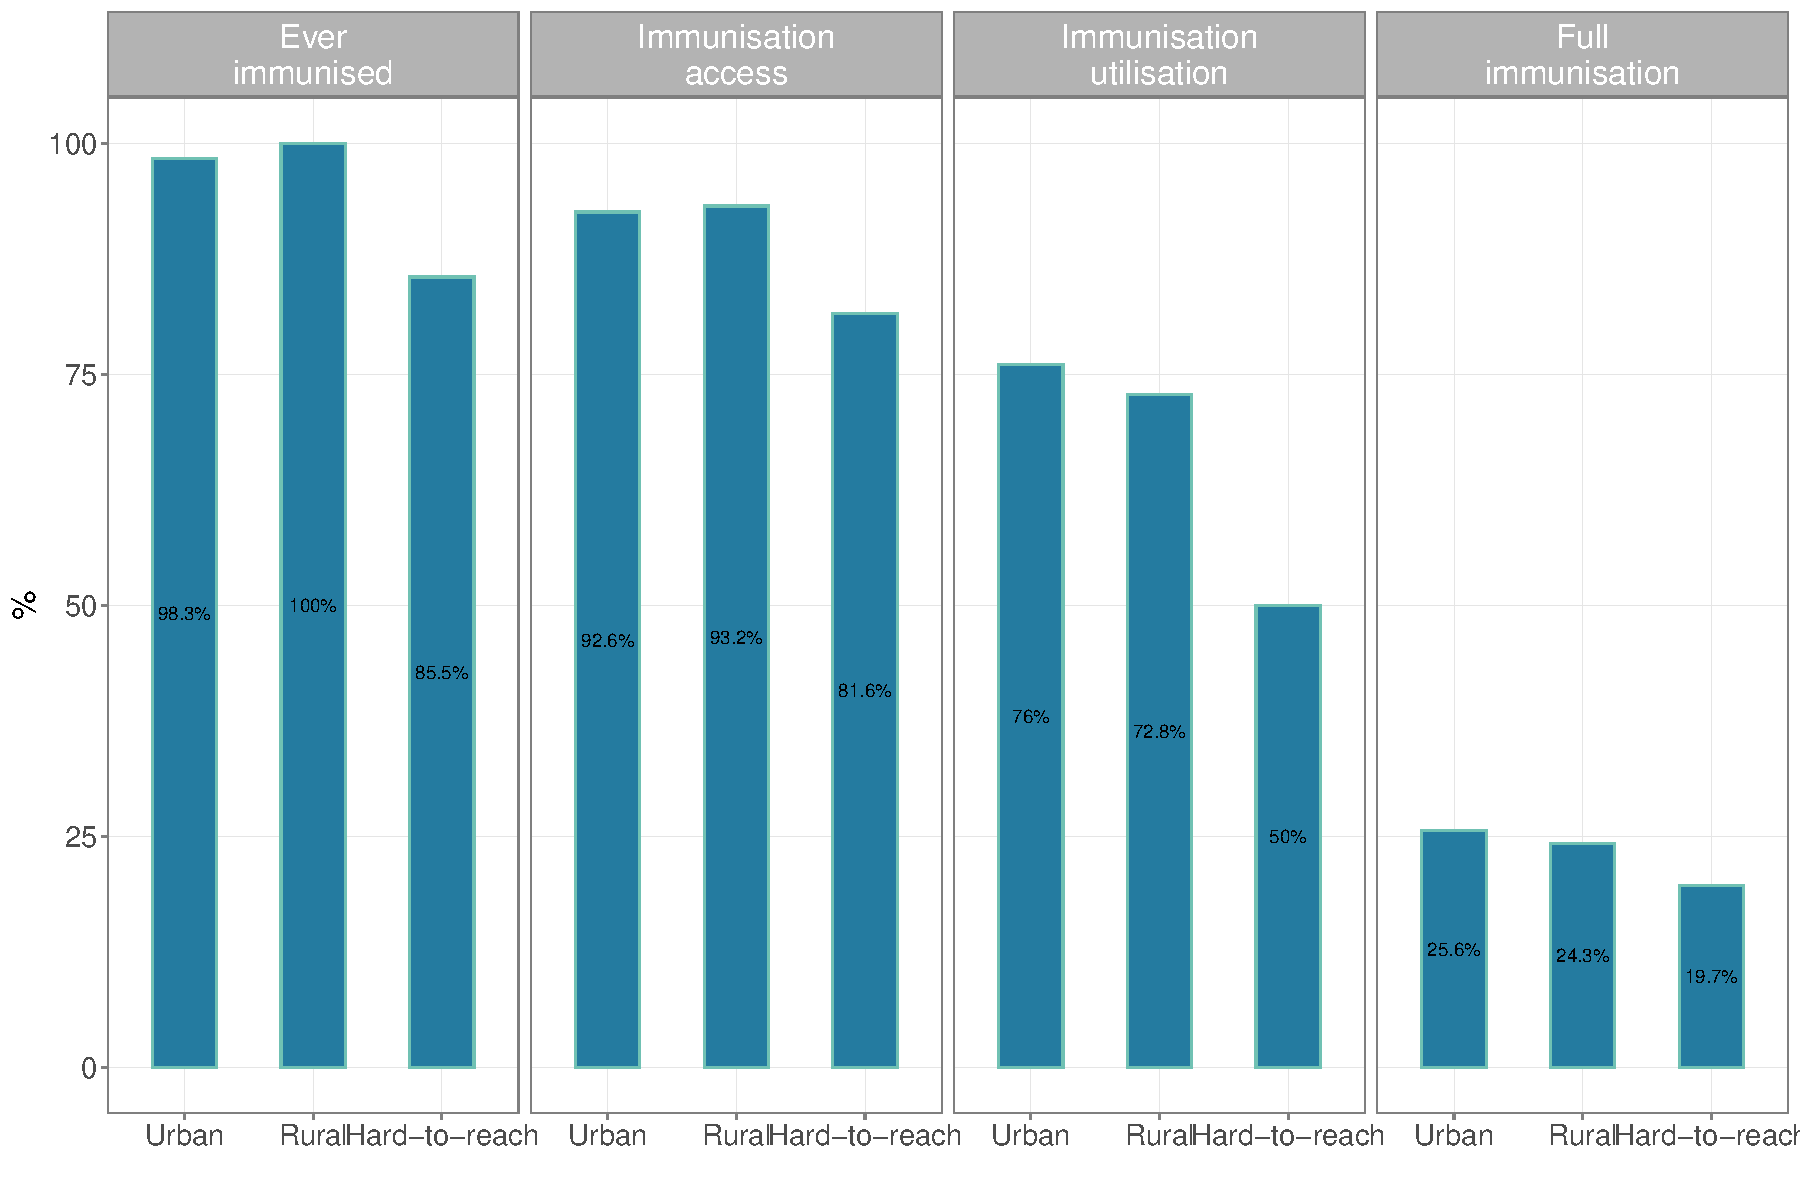
\includegraphics{kayinReport_files/figure-latex/epi1plot-1} 

}

\caption{Immunisation coverage by location type}\label{fig:epi1plot}
\end{figure}

\begin{figure}[H]

{\centering 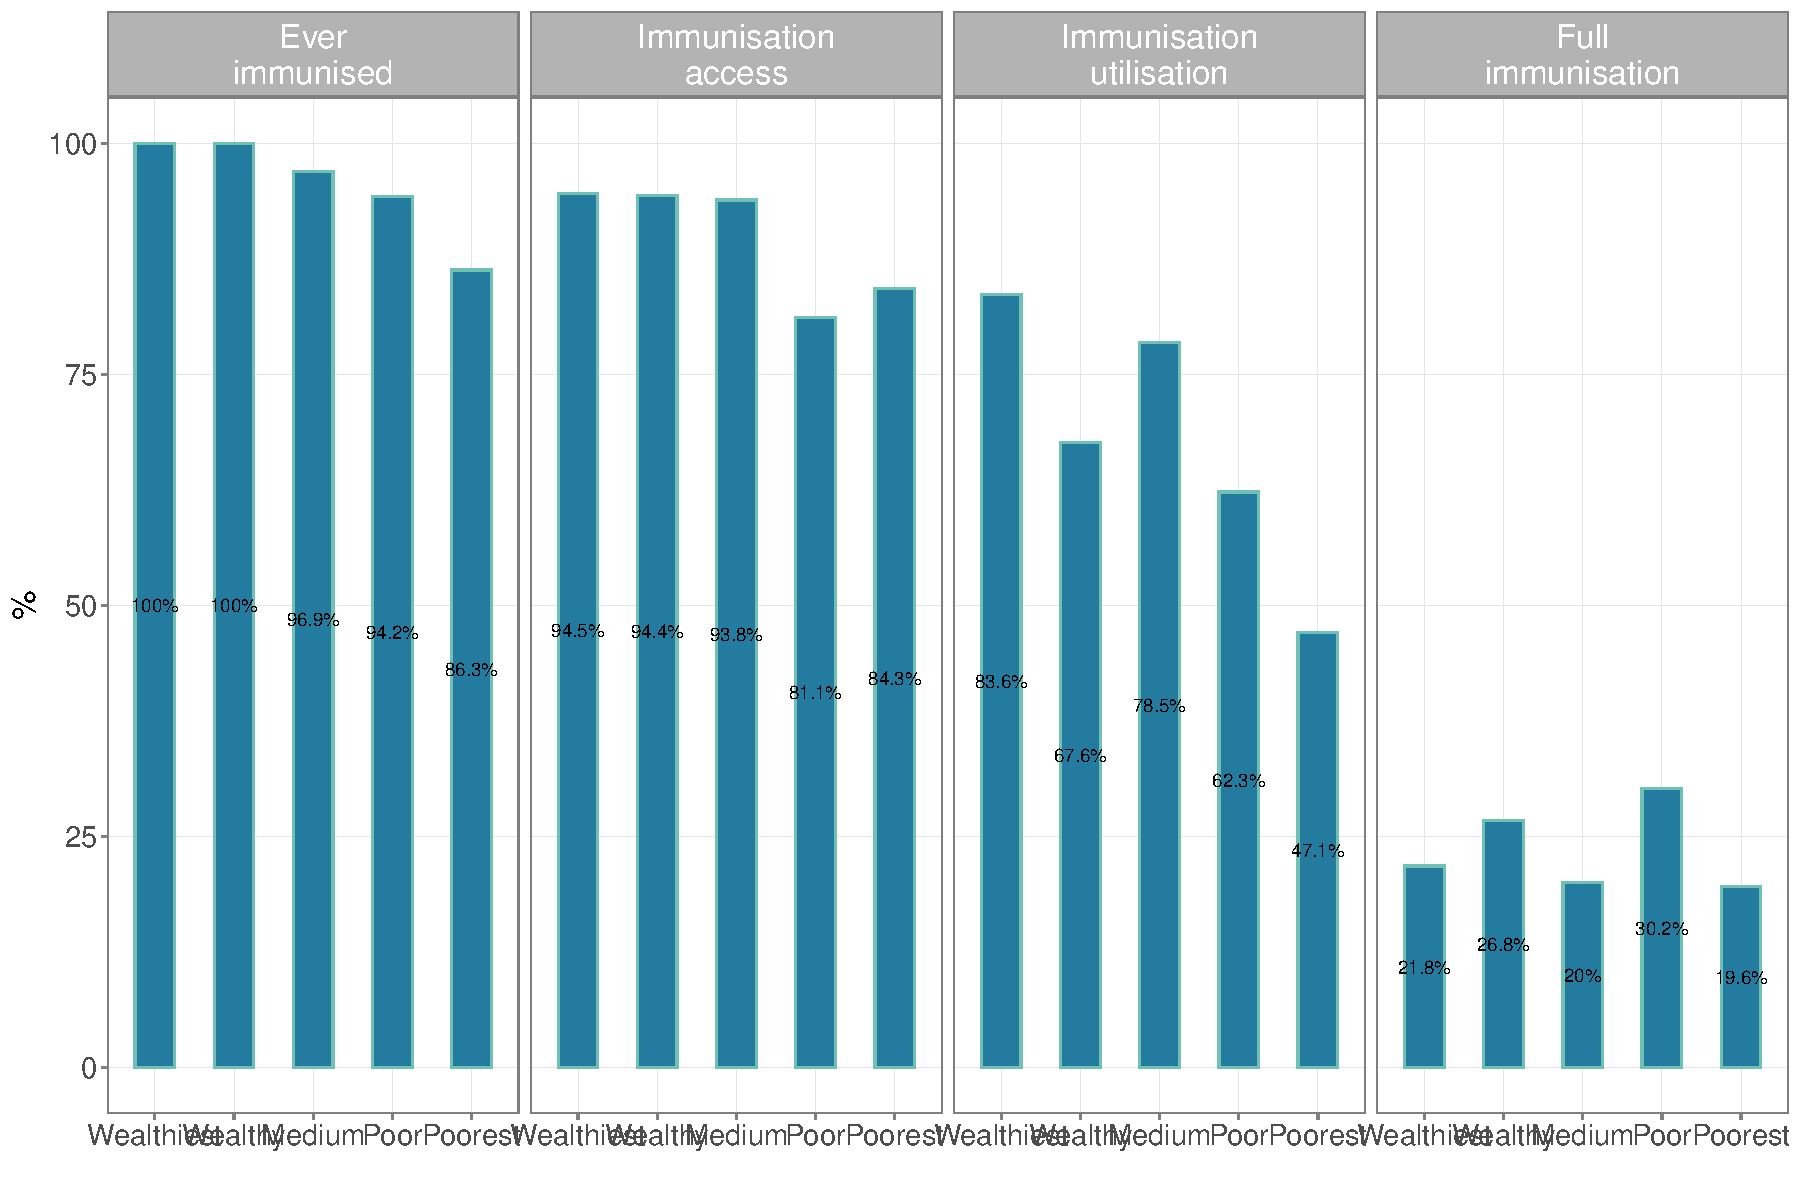
\includegraphics{kayinReport_files/figure-latex/epi2plot-1} 

}

\caption{Immunisation coverage by wealth quintiles}\label{fig:epi2plot}
\end{figure}

\begin{landscape}\begin{table}[H]

\caption{\label{tab:epi2table}Immunisation coverage per vaccine type}
\centering
\fontsize{9}{11}\selectfont
\begin{tabular}[t]{>{\bfseries}l>{\bfseries}l>{\ttfamily}r>{\ttfamily}r>{\ttfamily}r>{\ttfamily}r>{\ttfamily}r>{\ttfamily}r>{\ttfamily}r>{\ttfamily}r>{\ttfamily}r>{\ttfamily}r>{\ttfamily}r>{\ttfamily}r>{\ttfamily}r}
\toprule
 &  & \makecell[c]{BCG\\(\%)} & \makecell[c]{Hepatitis B\\(\%)} & \makecell[c]{Penta 1\\(\%)} & \makecell[c]{Penta 2\\(\%)} & \makecell[c]{Penta 3\\(\%)} & \makecell[c]{OPV 1\\(\%)} & \makecell[c]{OPV 2\\(\%)} & \makecell[c]{OPV 3\\(\%)} & \makecell[c]{IPV\\(\%)} & \makecell[c]{Measles 1\\(\%)} & \makecell[c]{Measles 2\\(\%)} & \makecell[c]{Rubella\\(\%)} & \makecell[c]{Pneumococcal\\(\%)}\\
\midrule
\addlinespace[0.3em]
\multicolumn{15}{l}{\textbf{Kayin}}\\
\addlinespace[0.3em]
\multicolumn{15}{l}{\textit{\textbf{Geographic}}}\\
\hspace{1em}\hspace{1em} & Rural & 21.1 & 13.4 & 22.0 & 21.4 & 19.6 & 22.0 & 21.8 & 20.9 & 14.5 & 20.3 & 13.4 & 13.0 & 10.6\\
\cmidrule{2-15}
\hspace{1em}\hspace{1em} & Urban & 21.5 & 14.8 & 21.7 & 21.5 & 19.4 & 22.5 & 21.3 & 19.6 & 16.5 & 18.7 & 9.0 & 11.3 & 10.6\\
\cmidrule{2-15}
\hspace{1em}\hspace{1em} & Hard-to-reach & 15.2 & 11.3 & 15.0 & 12.5 & 10.3 & 15.2 & 12.0 & 10.8 & 10.0 & 10.8 & 7.1 & 7.4 & 6.6\\
\cmidrule{2-15}
\addlinespace[0.3em]
\multicolumn{15}{l}{\textit{\textbf{Wealth}}}\\
\hspace{1em}\hspace{1em} & Wealthiest & 19.8 & 14.5 & 20.2 & 19.8 & 18.3 & 20.6 & 19.8 & 19.1 & 17.2 & 17.2 & 8.0 & 9.5 & 8.8\\
\cmidrule{2-15}
\hspace{1em}\hspace{1em} & Wealthy & 23.1 & 15.2 & 23.1 & 22.8 & 20.0 & 23.8 & 22.1 & 20.0 & 16.6 & 20.0 & 11.7 & 11.7 & 10.7\\
\cmidrule{2-15}
\hspace{1em}\hspace{1em} & Medium & 21.2 & 14.9 & 20.8 & 20.8 & 18.4 & 21.9 & 20.8 & 19.1 & 14.9 & 19.1 & 10.1 & 10.8 & 10.1\\
\cmidrule{2-15}
\hspace{1em}\hspace{1em} & Poor & 16.7 & 12.0 & 18.2 & 15.9 & 14.0 & 18.2 & 15.1 & 14.3 & 12.0 & 15.5 & 11.6 & 12.0 & 9.7\\
\cmidrule{2-15}
\hspace{1em}\hspace{1em} & Poorest & 16.5 & 9.6 & 16.5 & 14.2 & 12.6 & 16.1 & 15.3 & 14.2 & 8.8 & 12.3 & 7.7 & 9.2 & 7.7\\
\bottomrule
\end{tabular}
\end{table}
\end{landscape}

\begin{figure}[H]

{\centering 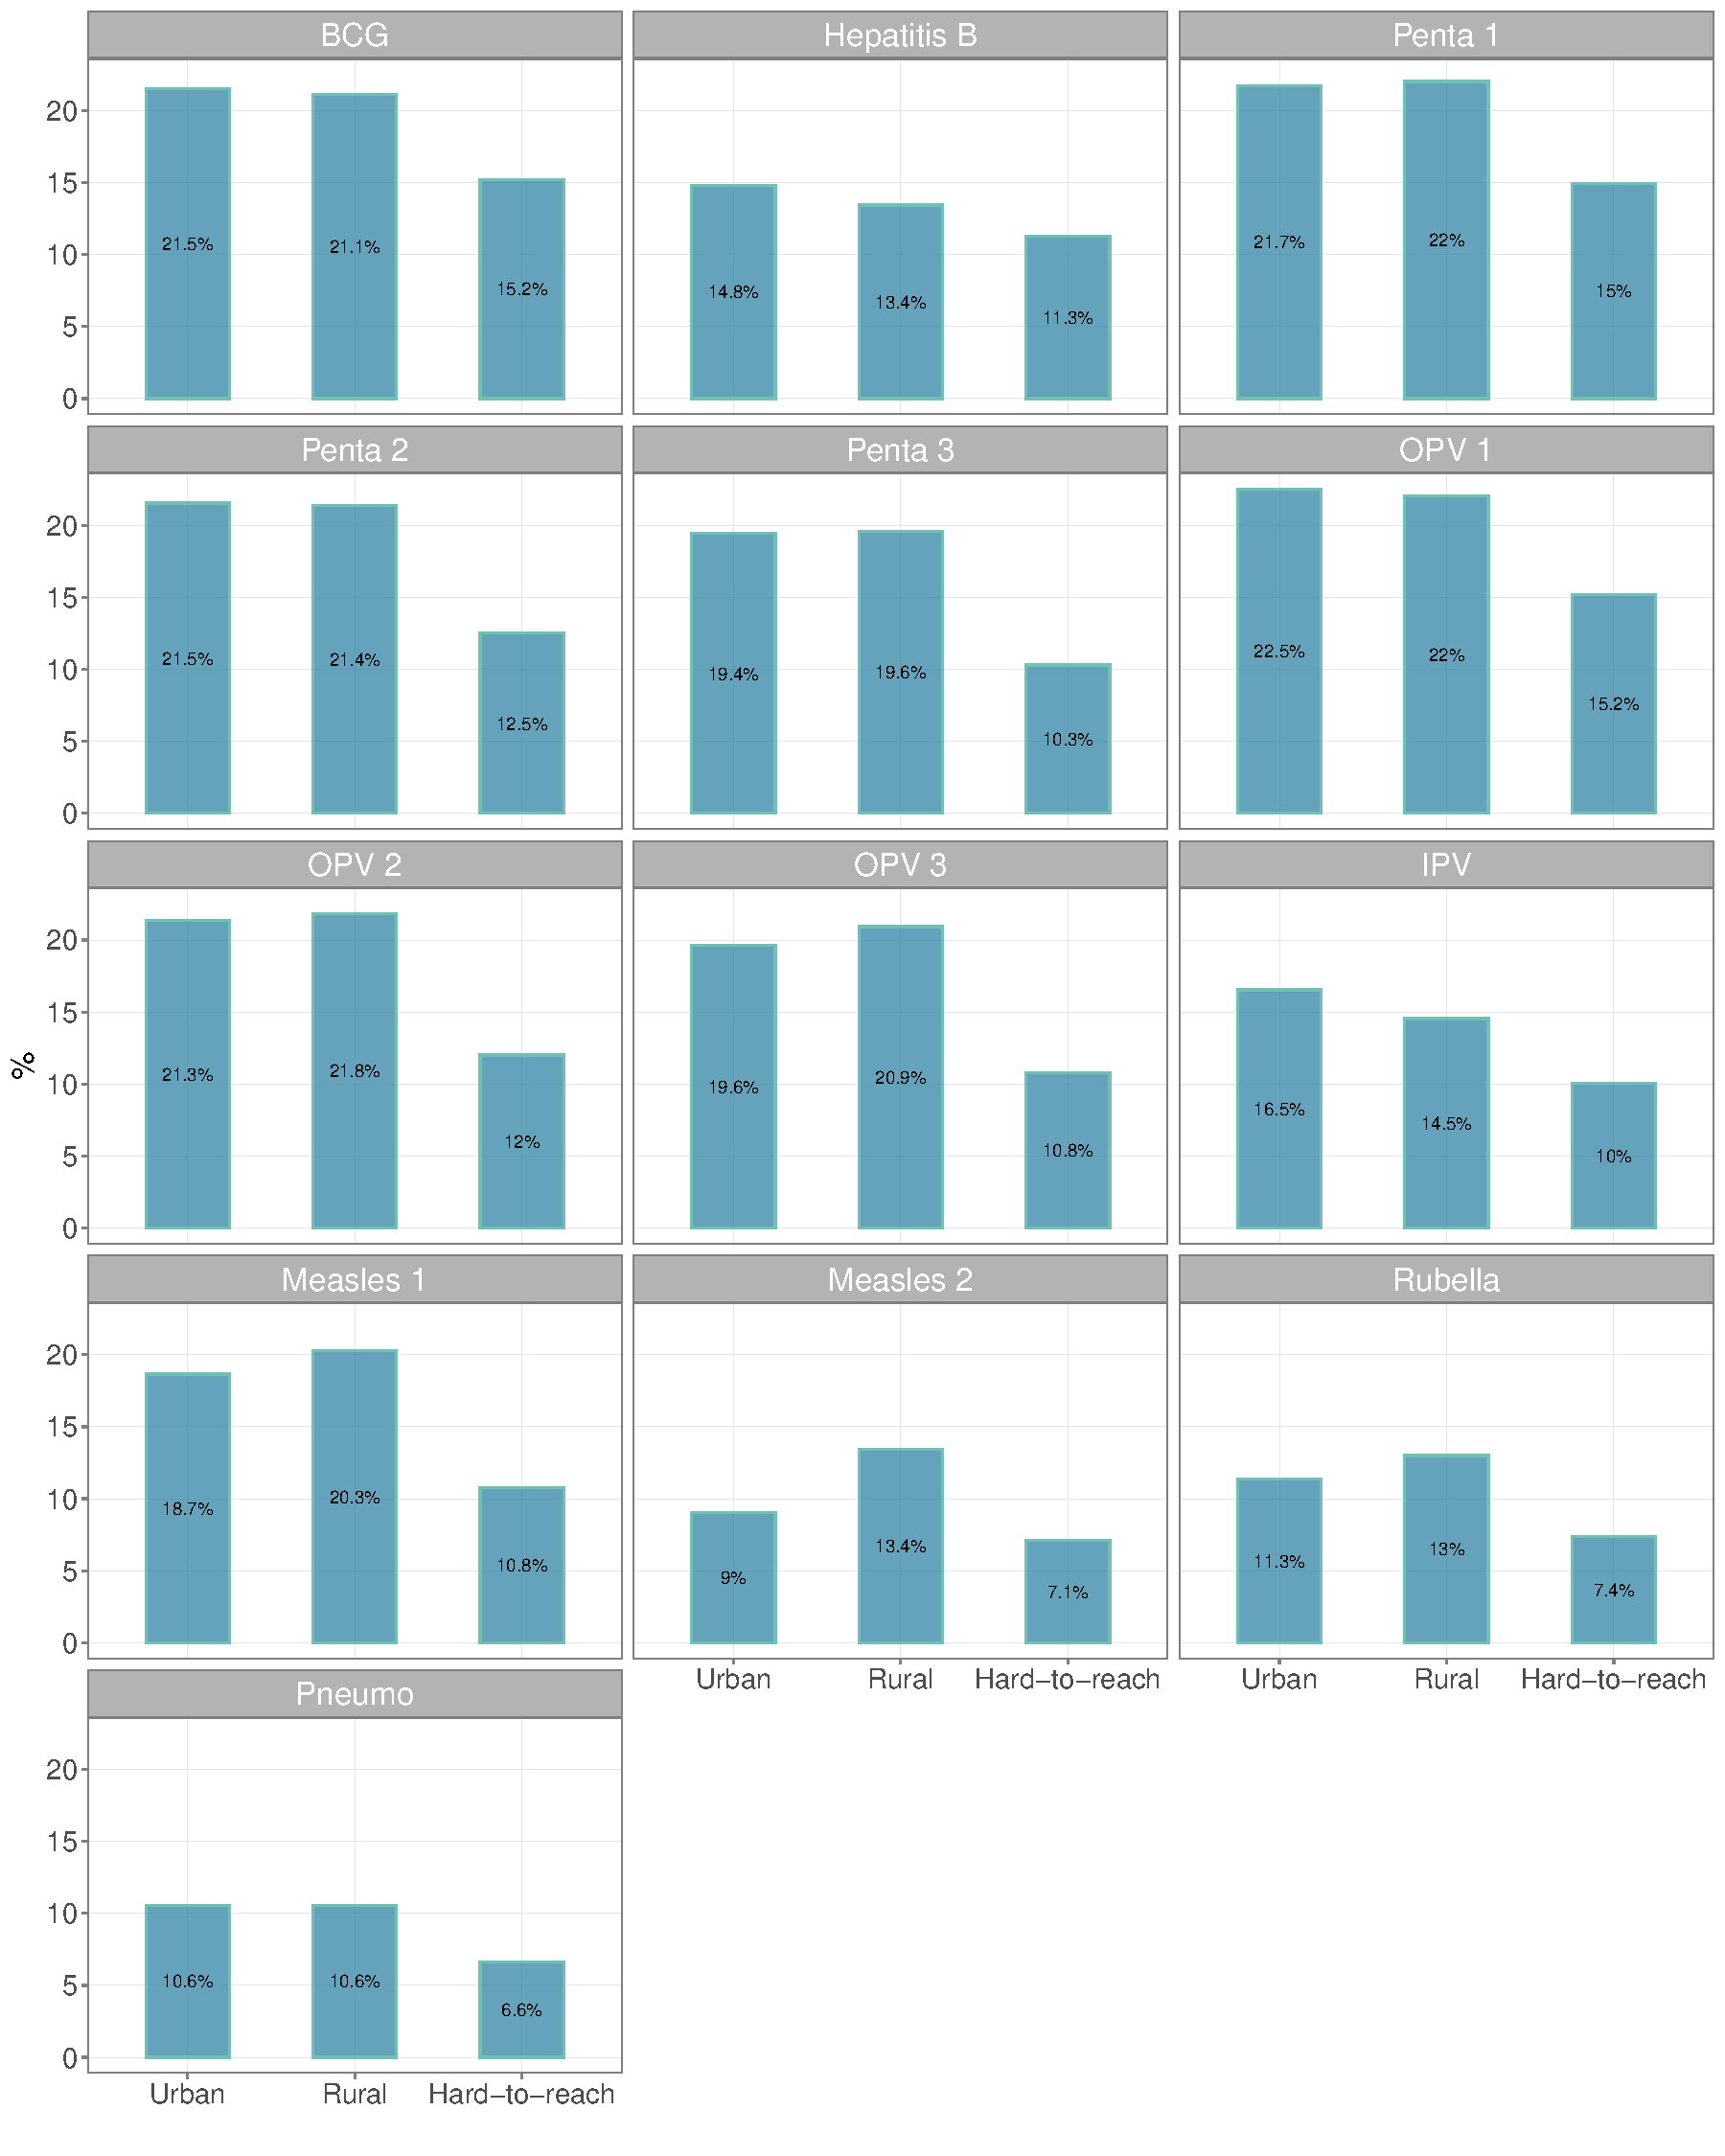
\includegraphics{kayinReport_files/figure-latex/epi3plot-1} 

}

\caption{Immunisation coverage per vaccine by location type}\label{fig:epi3plot}
\end{figure}

\begin{figure}[H]

{\centering 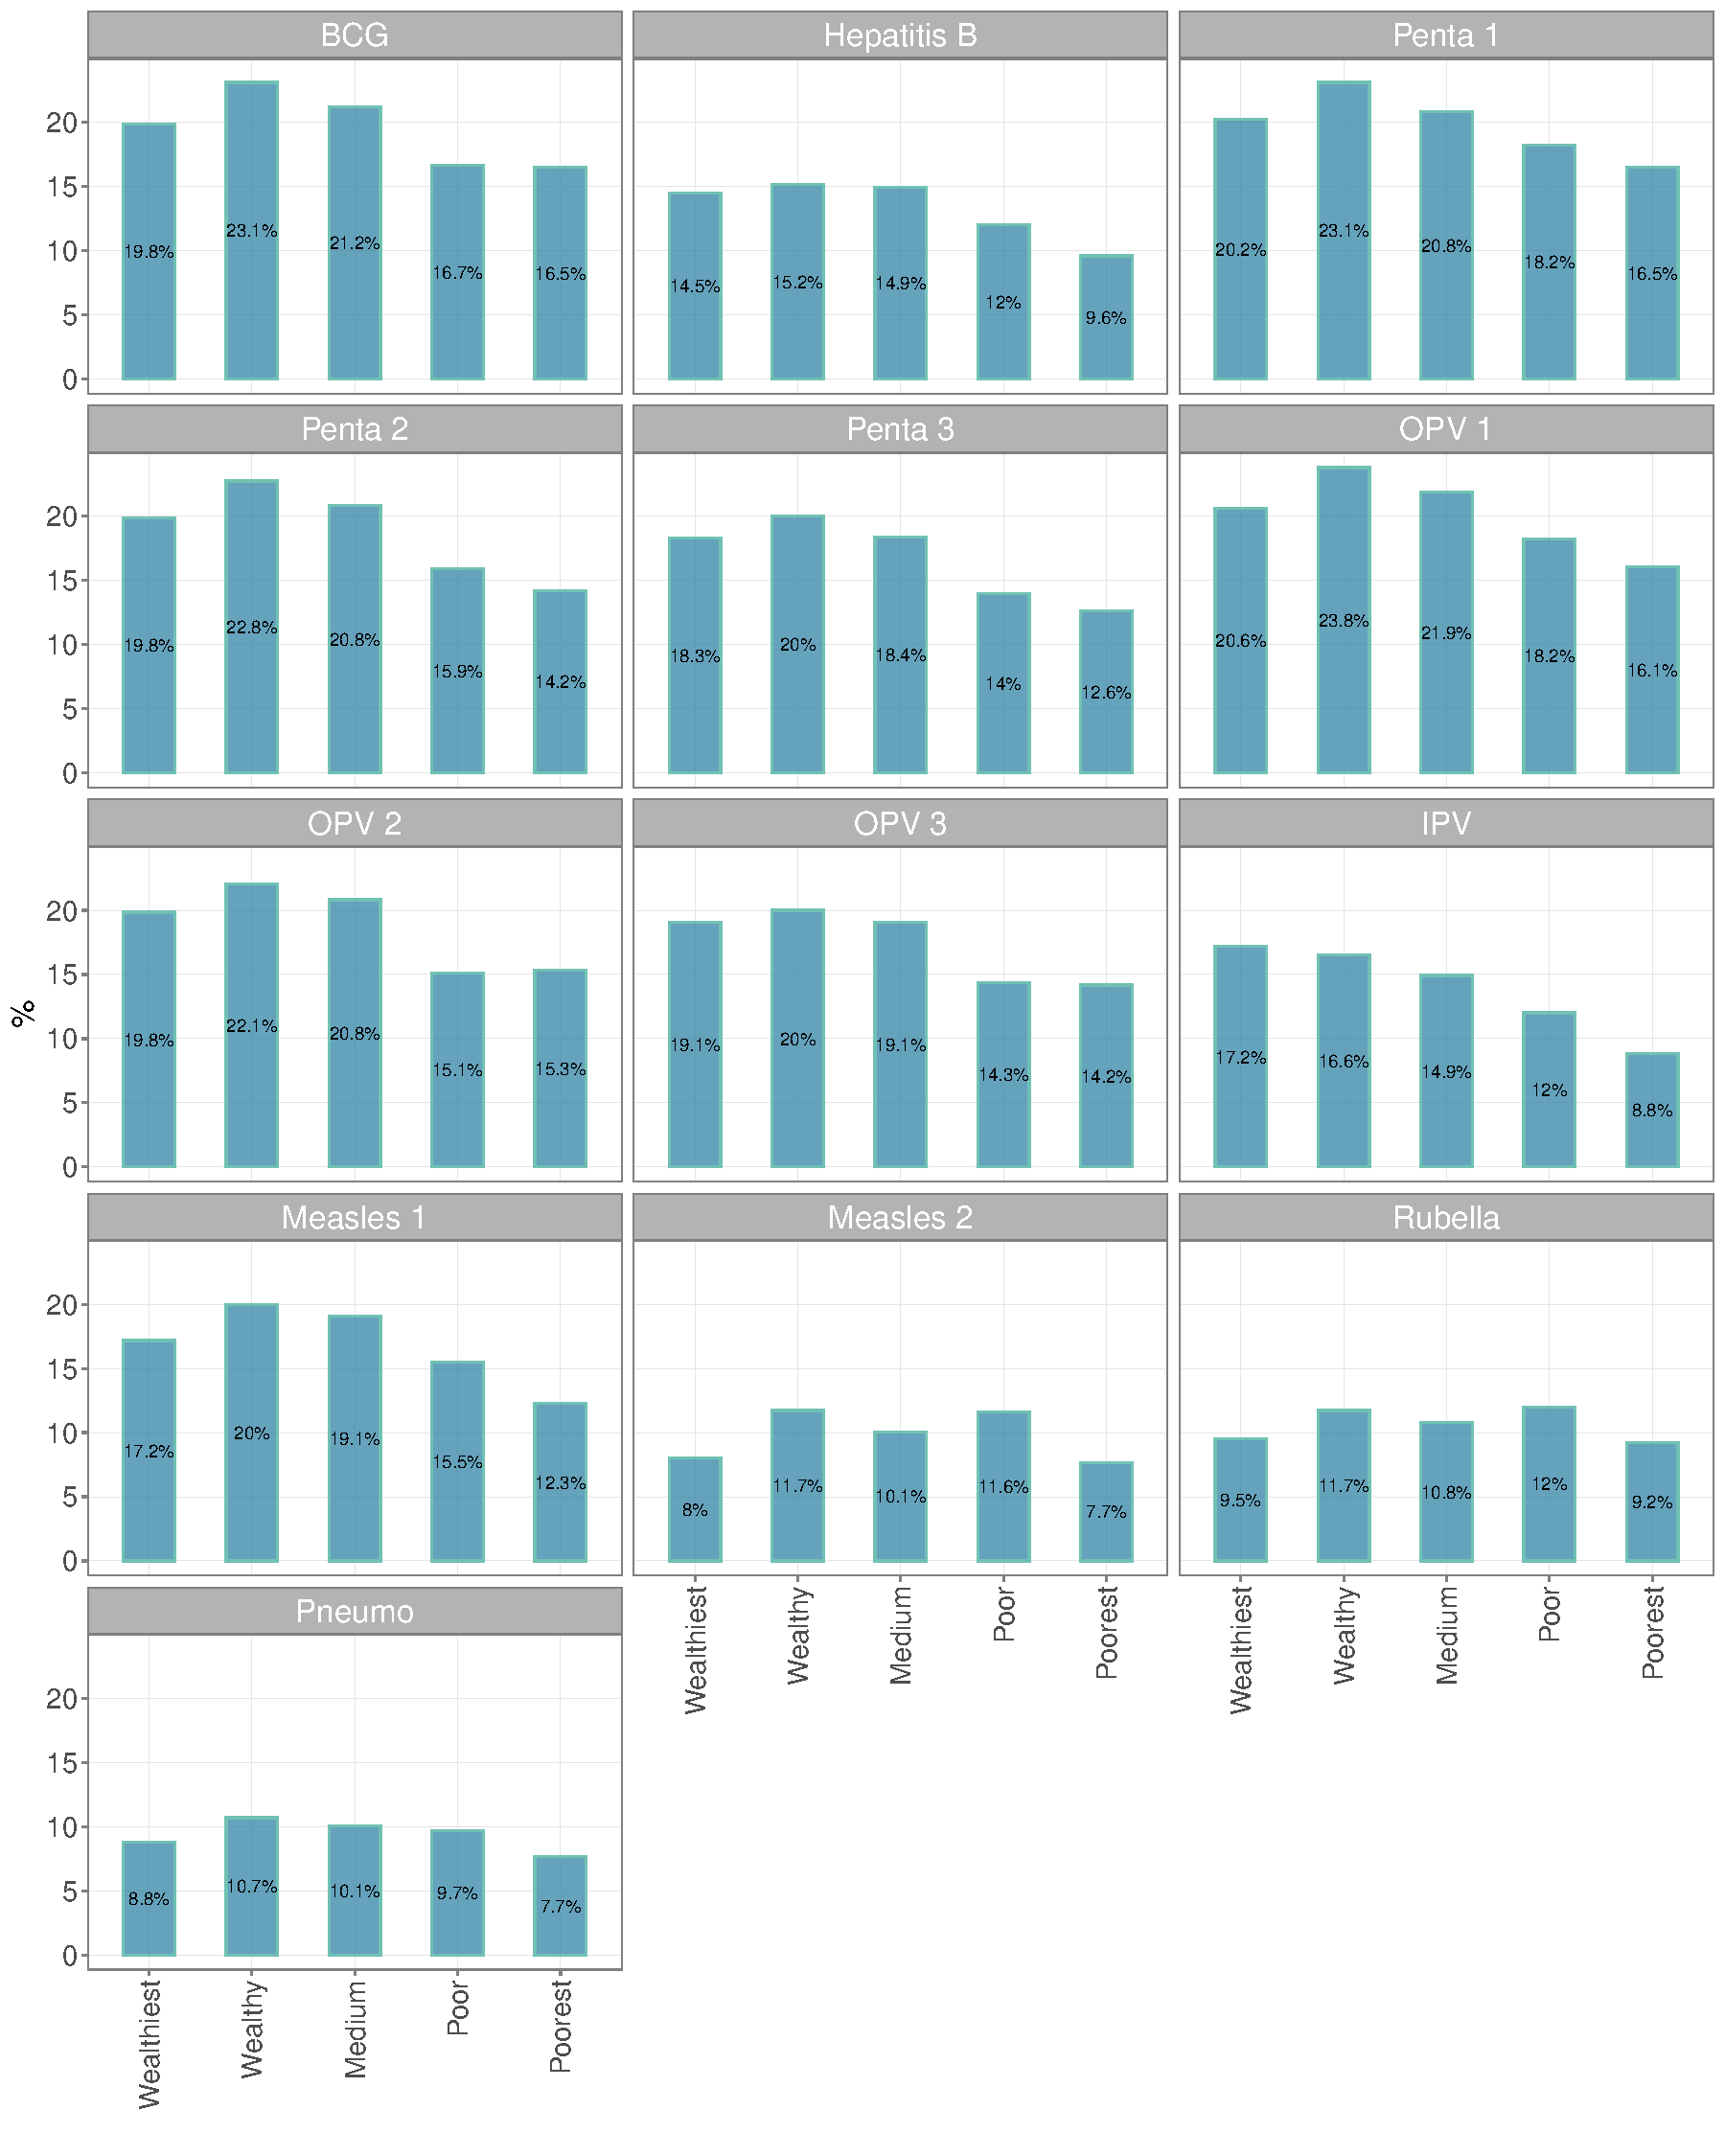
\includegraphics{kayinReport_files/figure-latex/epi4plot-1} 

}

\caption{Immunisation coverage per vaccine by wealth quintiles}\label{fig:epi4plot}
\end{figure}

Age-appropriate immunisation coverage per vaccine and overall (see Table \ref{tab:epi1aTable}, Figure \ref{fig:epi3aPlot} and \ref{fig:epi4aPlot}) show similar rates and trends across location types and wealth classes as the standard immunisation coverage indicators. This would indicate that the low levels of immunisaiton is a long-standing issue rather than just a current phenomenon.

\begin{landscape}\begin{table}[H]

\caption{\label{tab:epi1aTable}Age-appropriate immunisation coverage}
\centering
\fontsize{10}{12}\selectfont
\begin{tabular}[t]{>{\bfseries}l>{\bfseries}l>{\ttfamily}r>{\ttfamily}r>{\ttfamily}r>{\ttfamily}r>{\ttfamily}r>{\ttfamily}r>{\ttfamily}r>{\ttfamily}r>{\ttfamily}r>{\ttfamily}r>{\ttfamily}r>{\ttfamily}r>{\ttfamily}r}
\toprule
 &  & \makecell[c]{BCG\\(\%)} & \makecell[c]{Hepatitis B\\(\%)} & \makecell[c]{Penta 1\\(\%)} & \makecell[c]{Penta 2\\(\%)} & \makecell[c]{Penta 3\\(\%)} & \makecell[c]{Polio 1\\(\%)} & \makecell[c]{Polio 2\\(\%)} & \makecell[c]{Polio 3\\(\%)} & \makecell[c]{IPV\\(\%)} & \makecell[c]{Measles 1\\(\%)} & \makecell[c]{Measles 2\\(\%)} & \makecell[c]{Rubella\\(\%)} & \makecell[c]{Age-\\appropriate\\immunisation\\(\%)}\\
\midrule
\addlinespace[0.3em]
\multicolumn{15}{l}{\textbf{Kayin}}\\
\addlinespace[0.3em]
\multicolumn{15}{l}{\textit{\textbf{Geographic}}}\\
\hspace{1em}\hspace{1em} & Rural & 21.1 & 13.4 & 23.6 & 22.9 & 20.3 & 23.8 & 23.3 & 22.2 & 14.5 & 20.9 & 10.1 & 13.0 & 10.6\\
\cmidrule{2-15}
\hspace{1em}\hspace{1em} & Urban & 21.5 & 14.8 & 23.1 & 22.3 & 19.4 & 24.4 & 22.7 & 20.0 & 16.5 & 18.7 & 6.7 & 11.3 & 8.7\\
\cmidrule{2-15}
\hspace{1em}\hspace{1em} & Hard-to-reach & 15.2 & 11.3 & 22.3 & 16.4 & 11.5 & 23.8 & 18.6 & 14.0 & 10.0 & 12.5 & 4.7 & 7.4 & 3.7\\
\cmidrule{2-15}
\addlinespace[0.3em]
\multicolumn{15}{l}{\textit{\textbf{Wealth}}}\\
\hspace{1em}\hspace{1em} & Wealthiest & 19.8 & 14.5 & 21.4 & 20.2 & 18.7 & 22.1 & 21.0 & 19.8 & 17.2 & 17.2 & 5.3 & 9.5 & 6.5\\
\cmidrule{2-15}
\hspace{1em}\hspace{1em} & Wealthy & 23.1 & 15.2 & 25.2 & 24.1 & 20.3 & 25.9 & 23.4 & 20.7 & 16.6 & 20.0 & 8.6 & 11.7 & 9.3\\
\cmidrule{2-15}
\hspace{1em}\hspace{1em} & Medium & 21.2 & 14.9 & 23.6 & 22.6 & 18.8 & 25.0 & 23.3 & 21.2 & 14.9 & 19.4 & 7.3 & 10.8 & 8.0\\
\cmidrule{2-15}
\hspace{1em}\hspace{1em} & Poor & 16.7 & 12.0 & 22.9 & 18.6 & 15.1 & 23.6 & 19.8 & 16.3 & 12.0 & 16.3 & 9.3 & 12.0 & 8.9\\
\cmidrule{2-15}
\hspace{1em}\hspace{1em} & Poorest & 16.5 & 9.6 & 22.2 & 18.0 & 13.4 & 23.8 & 21.1 & 16.5 & 8.8 & 14.9 & 5.4 & 9.2 & 5.7\\
\bottomrule
\end{tabular}
\end{table}
\end{landscape}

\begin{figure}[H]

{\centering 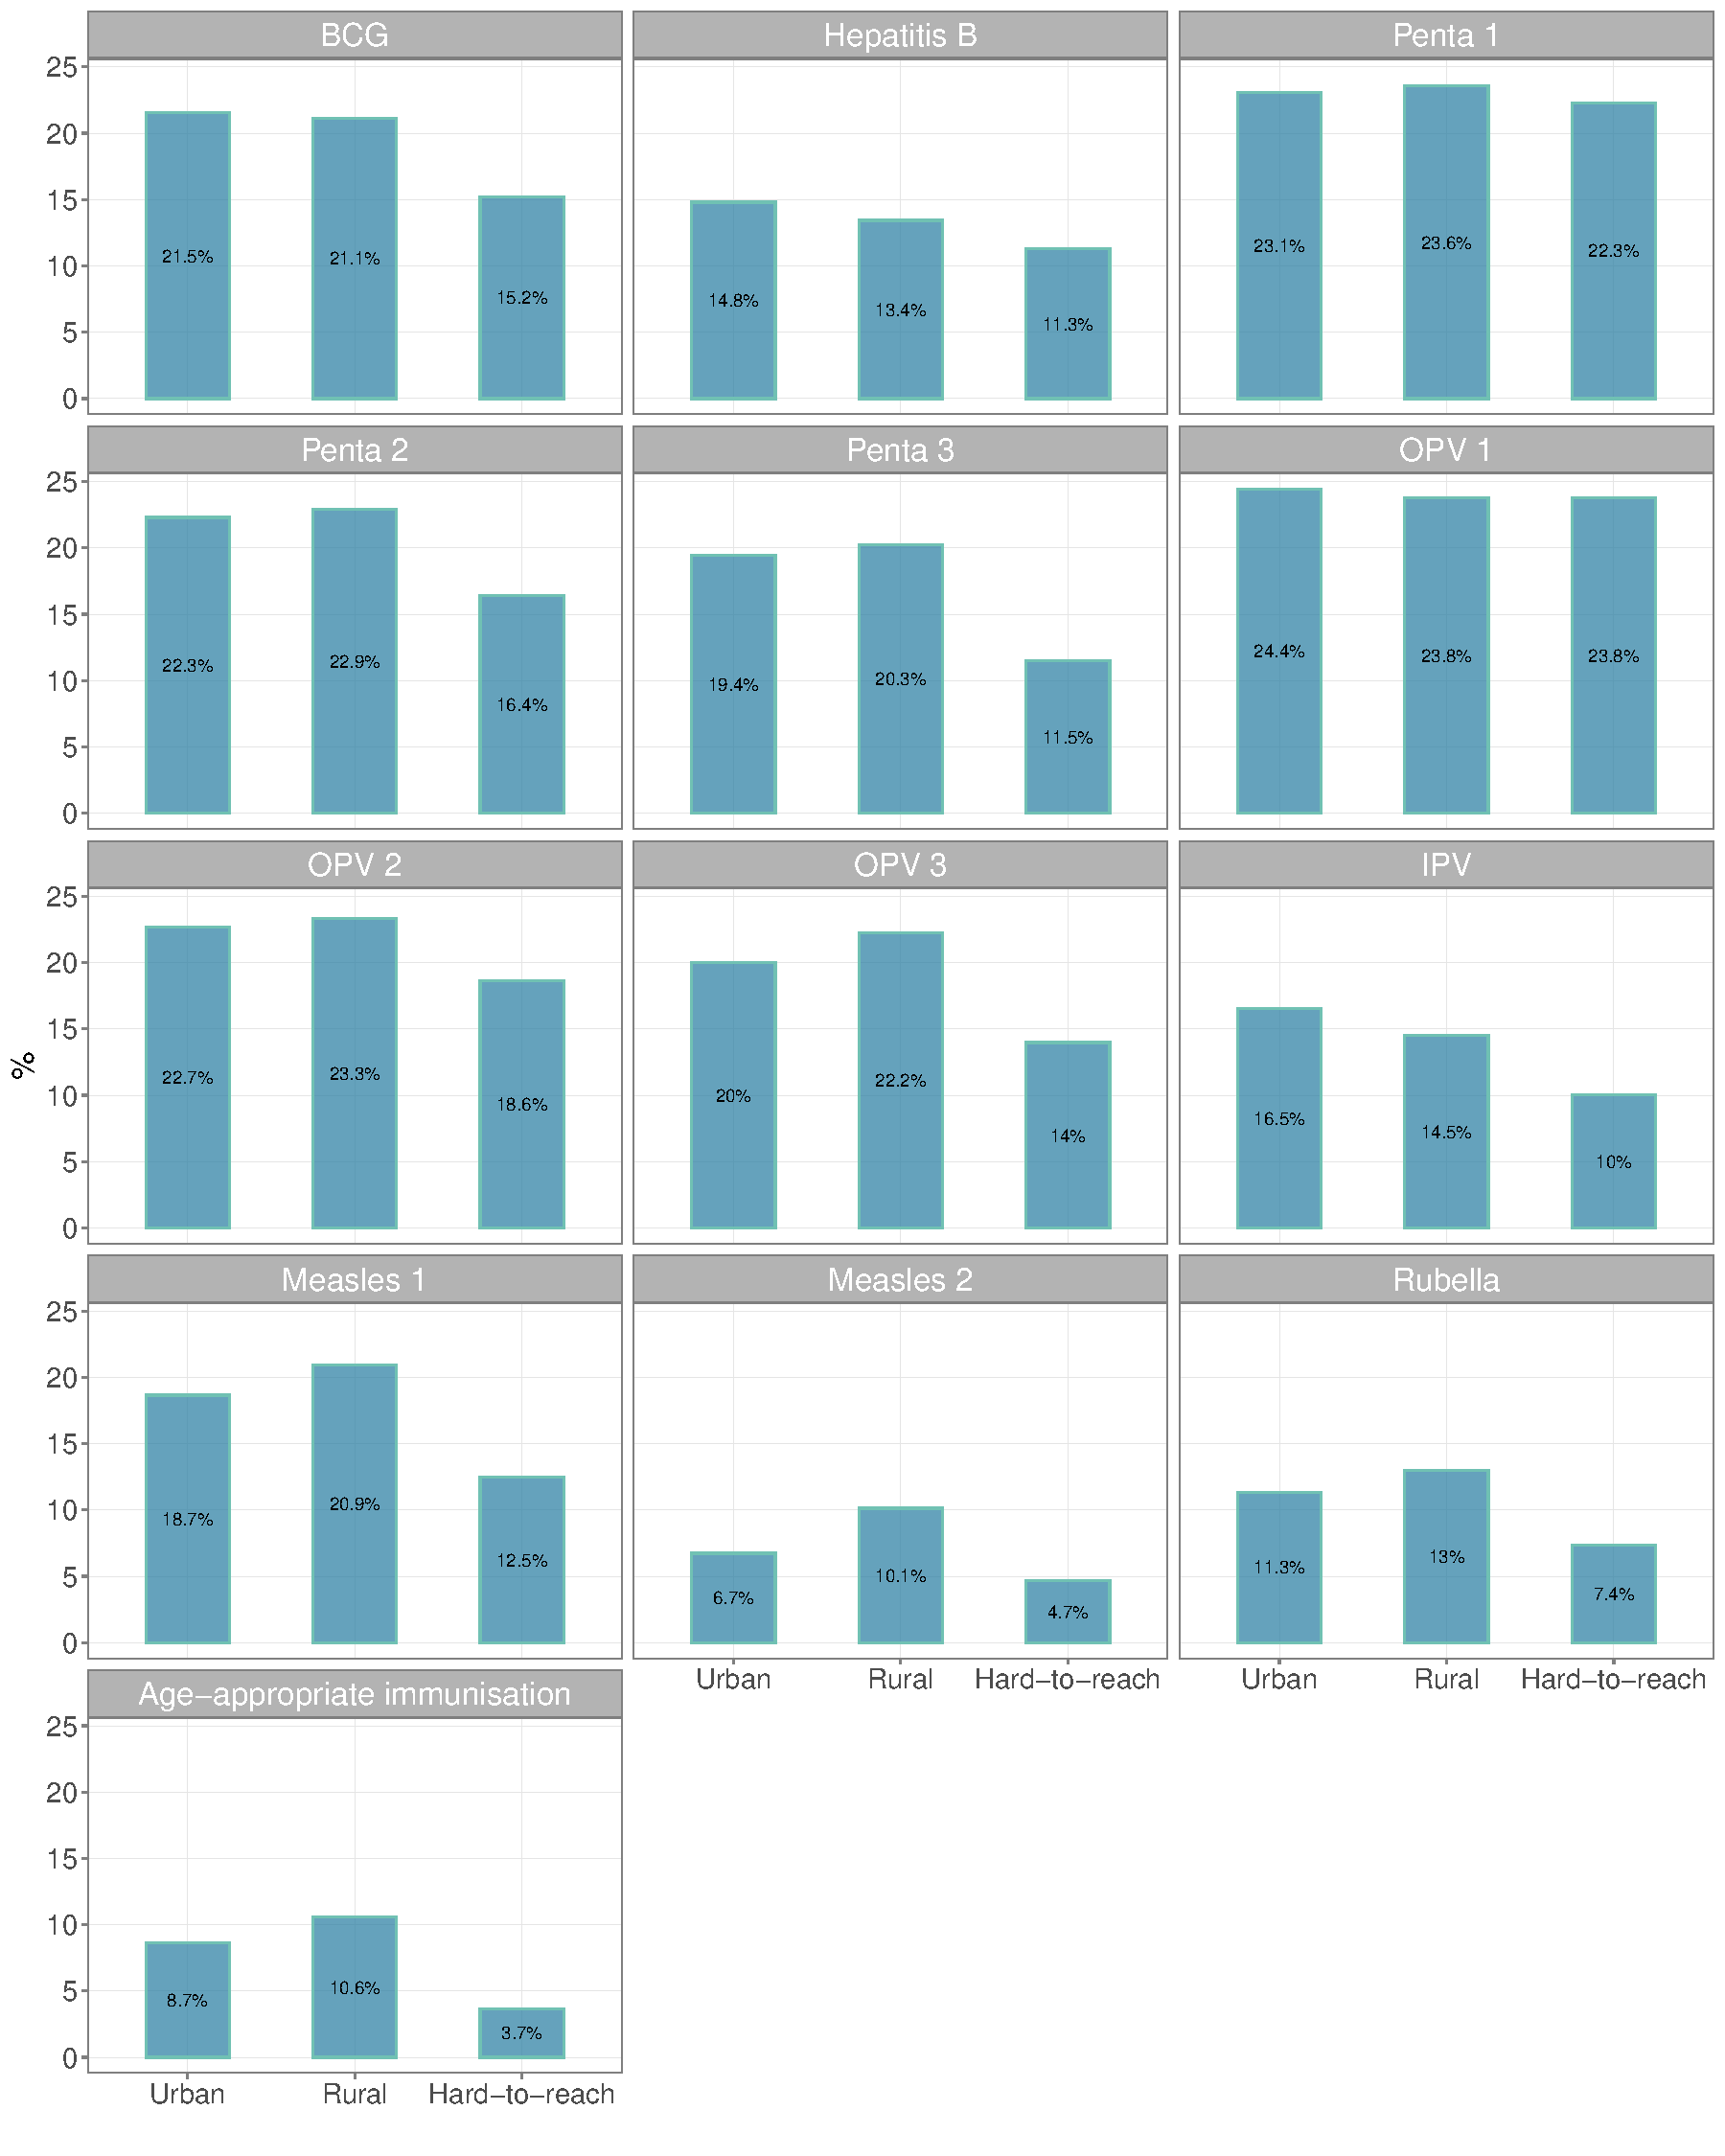
\includegraphics{kayinReport_files/figure-latex/epi3aPlot-1} 

}

\caption{Age-appropriate immunisation coverage per vaccine by location type}\label{fig:epi3aPlot}
\end{figure}

\begin{figure}[H]

{\centering 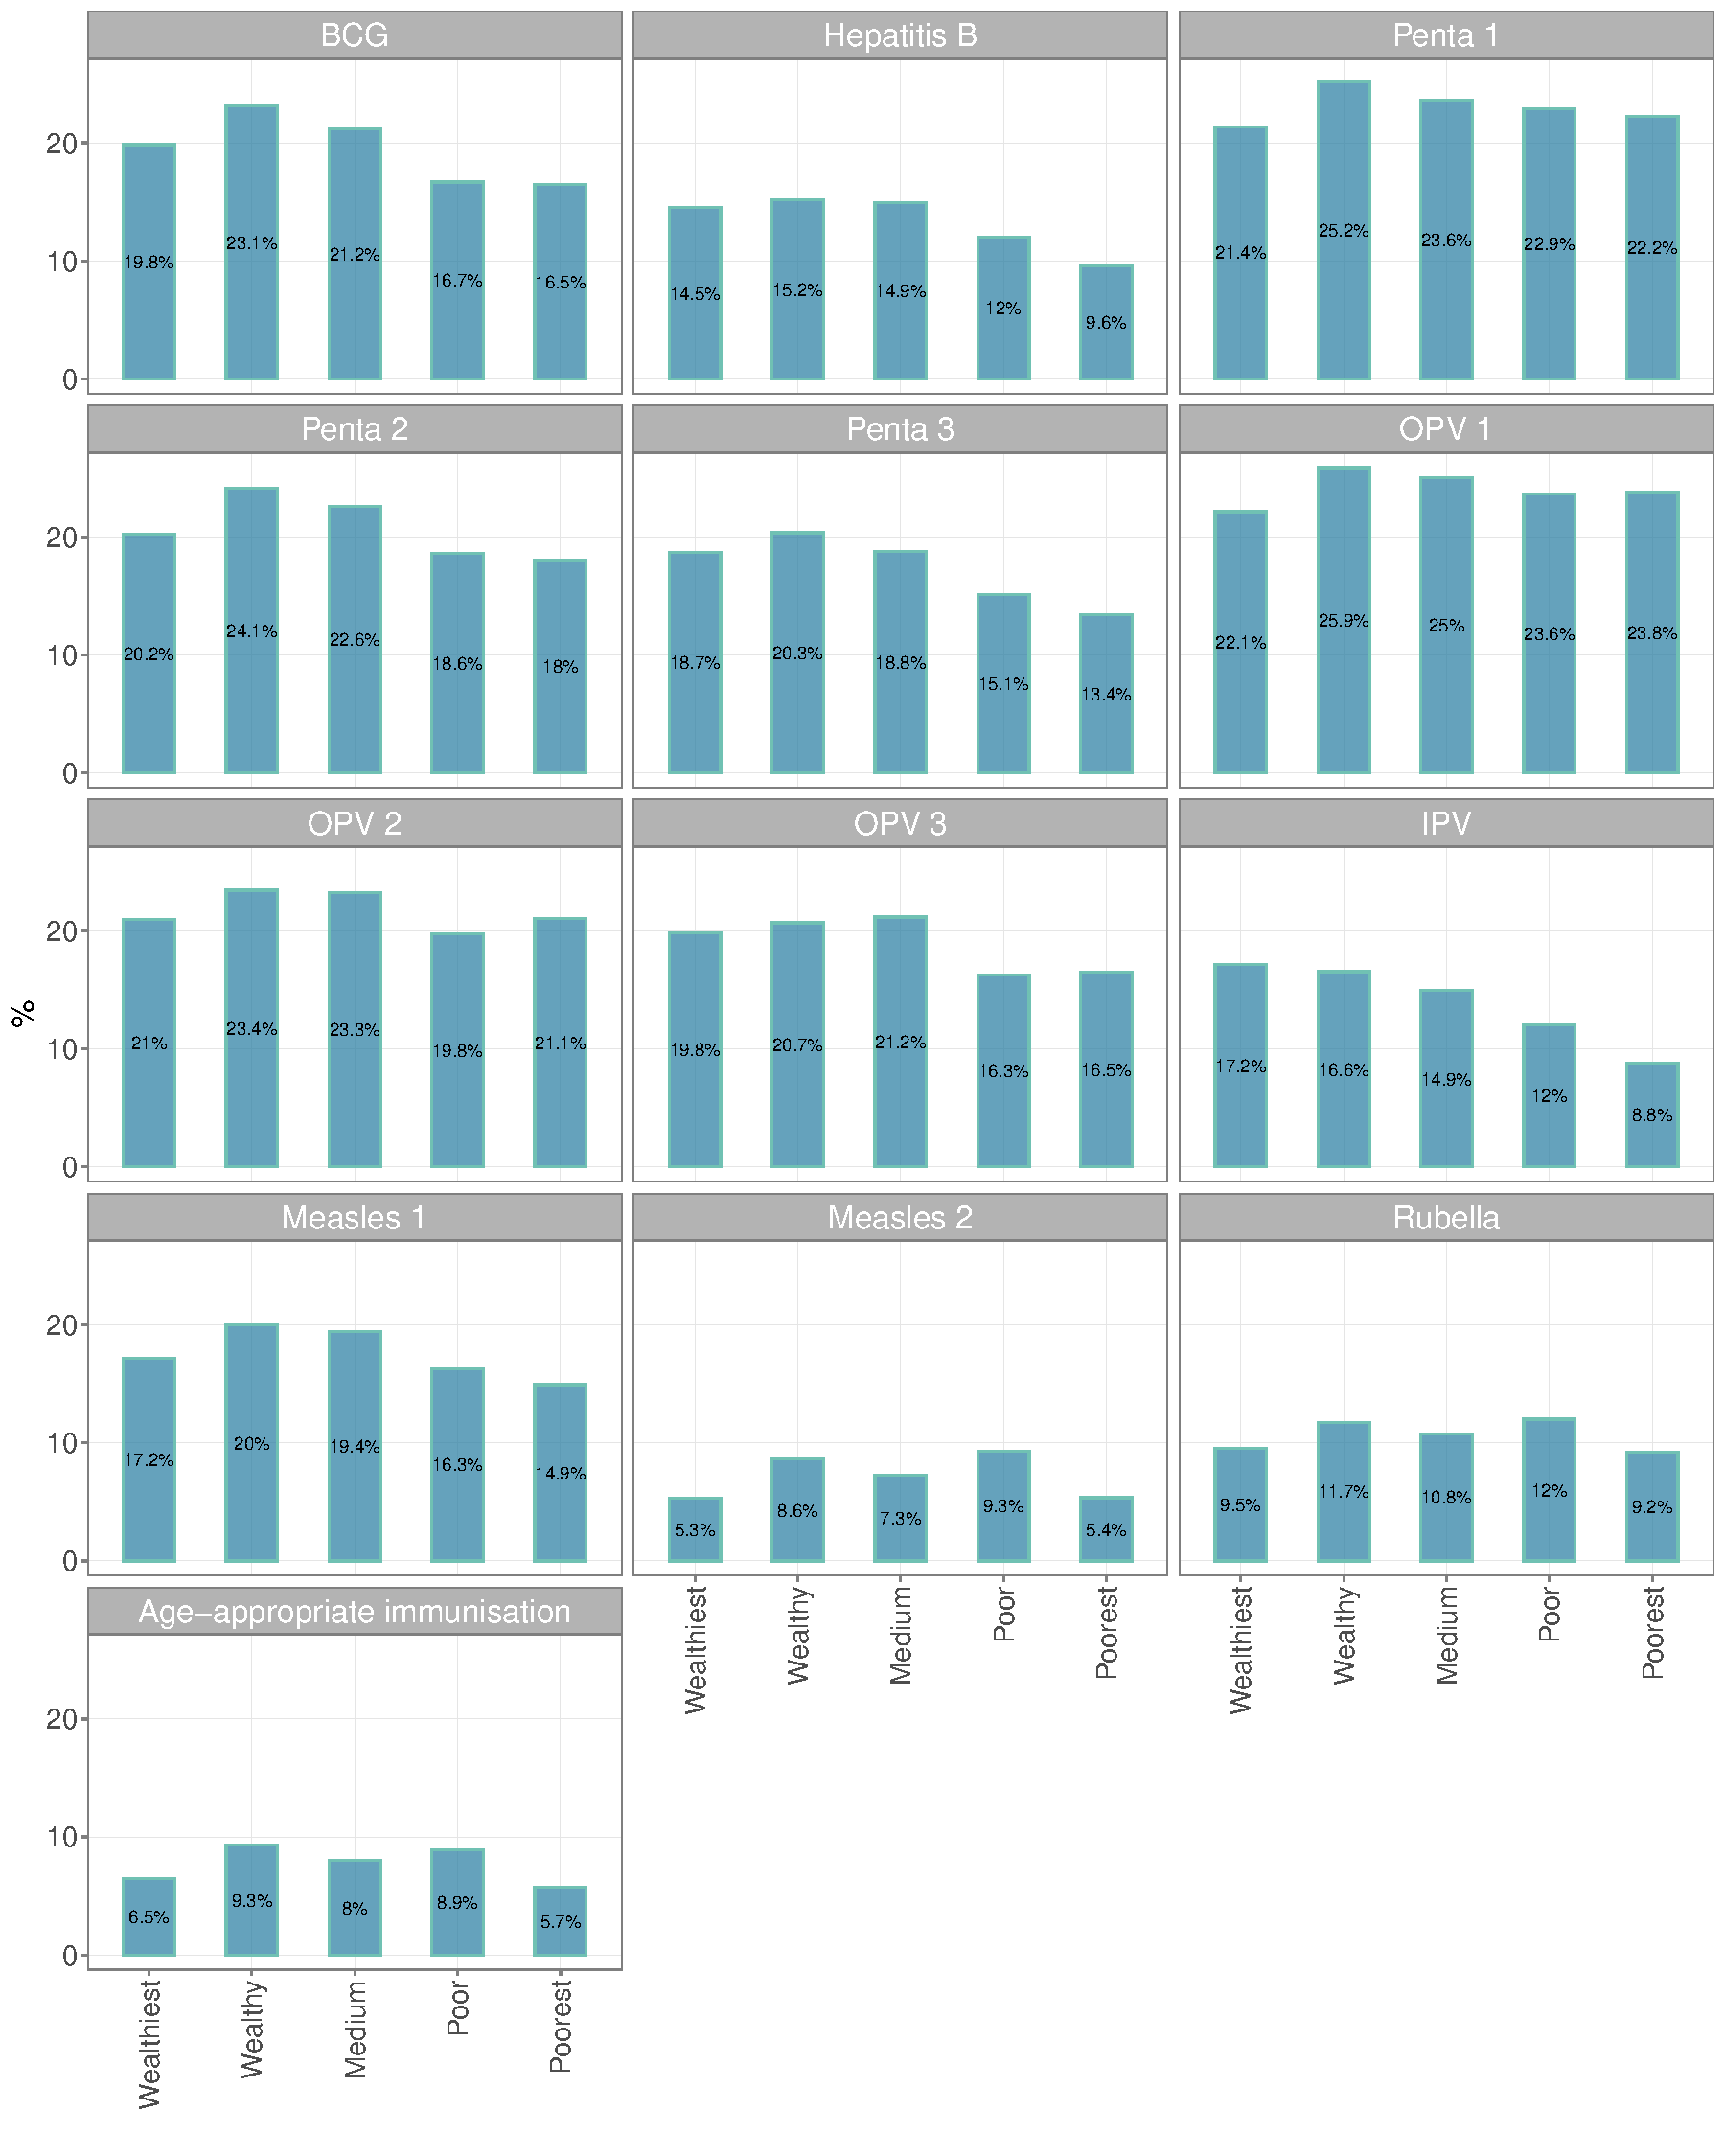
\includegraphics{kayinReport_files/figure-latex/epi4aPlot-1} 

}

\caption{Age-appropriate immunisation coverage per vaccine by wealth quintiles}\label{fig:epi4aPlot}
\end{figure}

\begin{table}[H]

\caption{\label{tab:epi3table}Coverage of immunisation-associated services}
\centering
\fontsize{12}{14}\selectfont
\begin{tabular}[t]{>{\bfseries}l>{\bfseries}l>{\ttfamily}r>{\ttfamily}r}
\toprule
 &  & \makecell[c]{Vitamin\\A\\supplementation\\(\%)} & \makecell[c]{Deworming\\(\%)}\\
\midrule
\addlinespace[0.3em]
\multicolumn{4}{l}{\textbf{Kayin}}\\
\addlinespace[0.3em]
\multicolumn{4}{l}{\textit{\textbf{Geographic}}}\\
\hspace{1em}\hspace{1em} & Rural & 56.5 & 24.9\\
\cmidrule{2-4}
\hspace{1em}\hspace{1em} & Urban & 35.8 & 10.9\\
\cmidrule{2-4}
\hspace{1em}\hspace{1em} & Hard-to-reach & 26.5 & 13.8\\
\cmidrule{2-4}
\addlinespace[0.3em]
\multicolumn{4}{l}{\textit{\textbf{Wealth}}}\\
\hspace{1em}\hspace{1em} & Wealthiest & 33.6 & 11.5\\
\cmidrule{2-4}
\hspace{1em}\hspace{1em} & Wealthy & 40.3 & 15.5\\
\cmidrule{2-4}
\hspace{1em}\hspace{1em} & Medium & 40.2 & 15.6\\
\cmidrule{2-4}
\hspace{1em}\hspace{1em} & Poor & 41.1 & 15.9\\
\cmidrule{2-4}
\hspace{1em}\hspace{1em} & Poorest & 36.6 & 22.0\\
\bottomrule
\end{tabular}
\end{table}

\begin{figure}[H]

{\centering 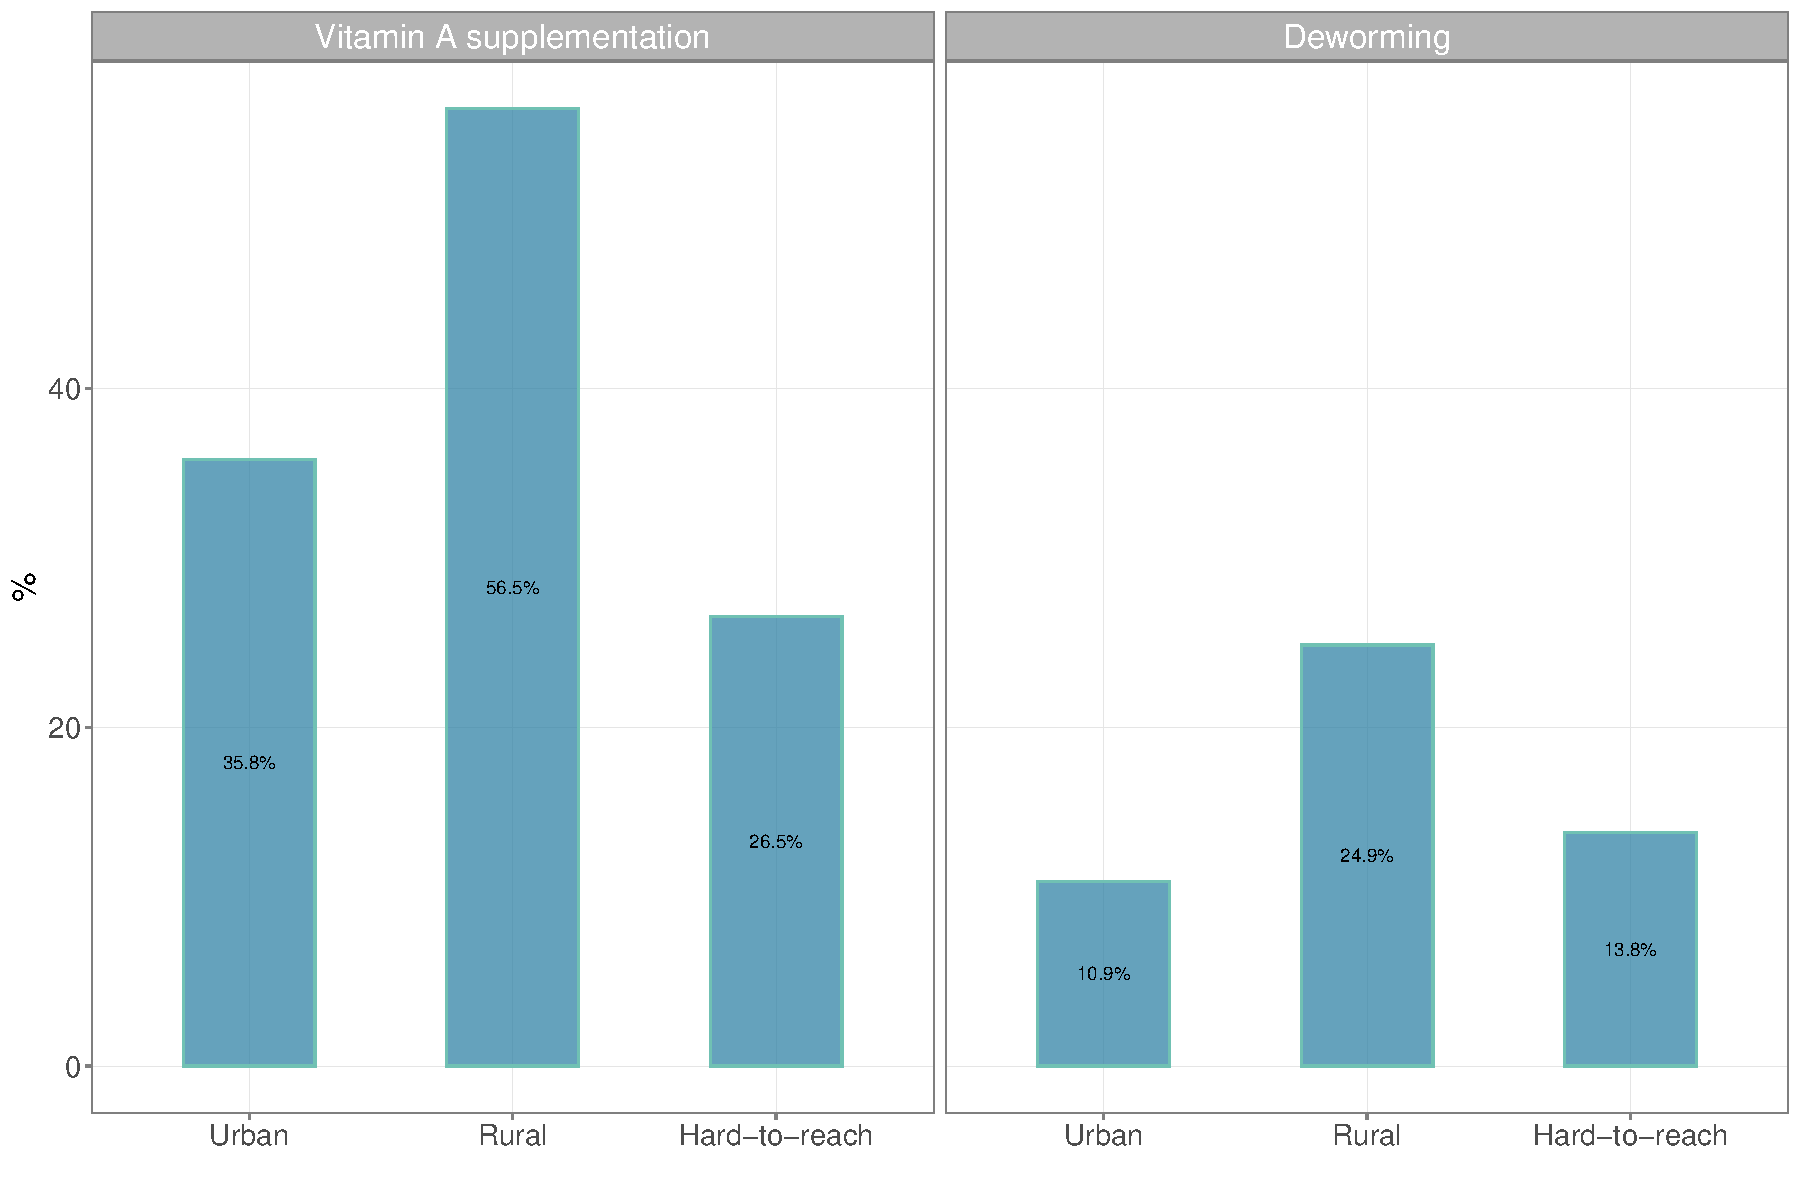
\includegraphics{kayinReport_files/figure-latex/epi5plot-1} 

}

\caption{Immunisation-associated services coverage by location type}\label{fig:epi5plot}
\end{figure}

\begin{figure}[H]

{\centering 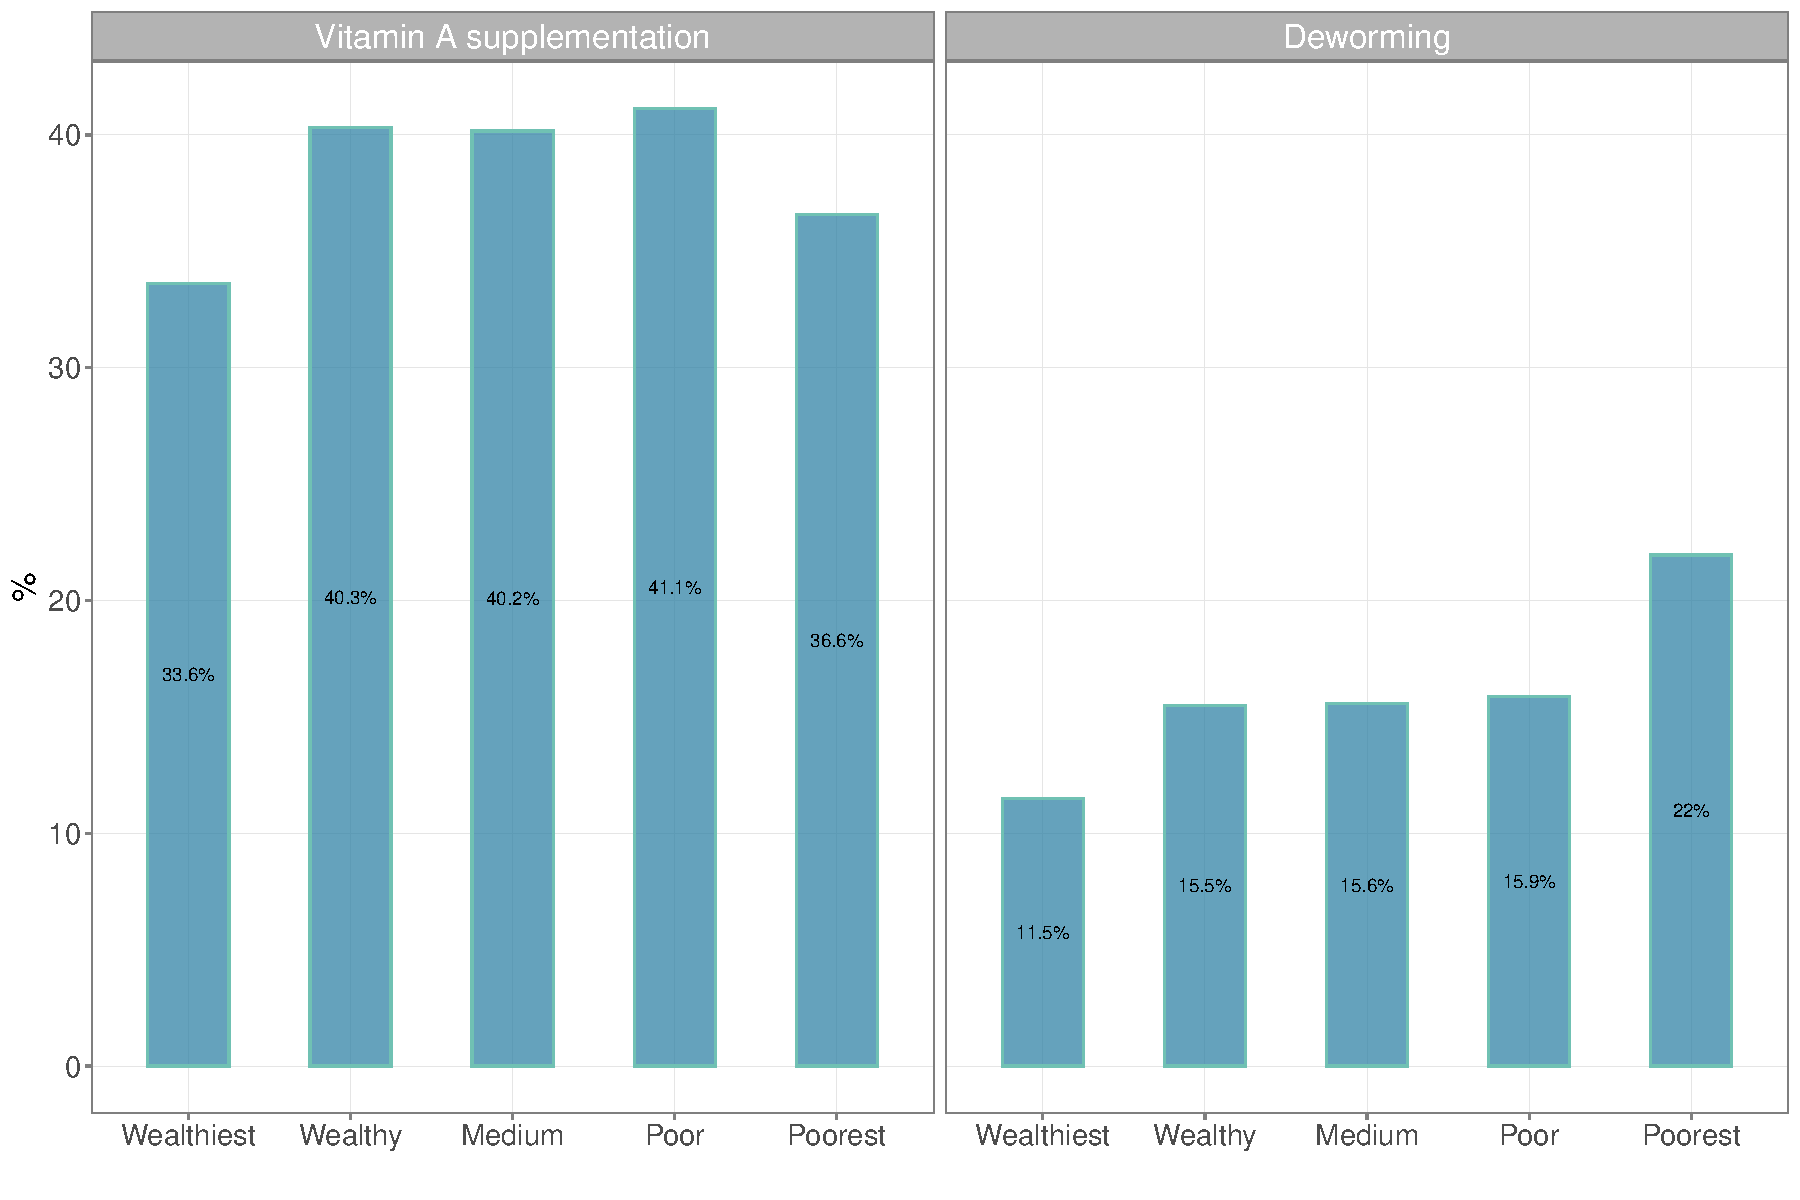
\includegraphics{kayinReport_files/figure-latex/epi6plot-1} 

}

\caption{Immunisation-associated services coverage by wealth quintiles}\label{fig:epi6plot}
\end{figure}

\hypertarget{illness}{%
\paragraph{Period prevalence of childhood illnesses}\label{illness}}

Fever is the most self-reported illness in children 6-59 months old with up to 29\% of mothers reporting fever in their children in the past 2 weeks in rural areas followed closely by those in urban areas at 26\% and by 18\% of mothers in hard-to-reach areas (see Figure \ref{fig:ill1plot}). The wealthier households also report fever the most at 27\% compared to 19\% for poor and 21\% for poorest households (see Figure \ref{fig:ill2plot}).

ARI is the next most self-reported illness in children 6-59 months old with up to 11\% of mothers in hard-to-reach areas reporting ARI in their children in the past 2 weeks (see Figure \ref{fig:ill1plot}. No clear trend by wealth classes can be observed with self-reporting of ARI (see Figure \ref{fig:ill2plot}).

Diarrhoea is the least self-reported illness in children 6-59 months old with 2\% of mothers in urban areas reporting cough in their children in the past 2 weeks. Those in rural and hard-to-reach areas report diarrhoea the most at 3\% (see Figure \ref{fig:ill1plot}. The poorest households reported the most diarrhoea in children at 5\% (see Figure \ref{fig:ill2plot}).

\begin{table}[H]

\caption{\label{tab:ill1table}Period prevalence of childhood illnesses}
\centering
\fontsize{12}{14}\selectfont
\begin{tabular}[t]{>{\bfseries}l>{\bfseries}l>{\ttfamily}r>{\ttfamily}r>{\ttfamily}r}
\toprule
 &  & \makecell[c]{Diarrhoea\\(\%)} & \makecell[c]{ARI\\(\%)} & \makecell[c]{Fever\\(\%)}\\
\midrule
\addlinespace[0.3em]
\multicolumn{5}{l}{\textbf{Kayin}}\\
\addlinespace[0.3em]
\multicolumn{5}{l}{\textit{\textbf{Geographic}}}\\
\hspace{1em}\hspace{1em} & Rural & 3.2 & 9.0 & 28.5\\
\cmidrule{2-5}
\hspace{1em}\hspace{1em} & Urban & 1.6 & 8.1 & 25.8\\
\cmidrule{2-5}
\hspace{1em}\hspace{1em} & Hard-to-reach & 2.9 & 11.3 & 18.0\\
\cmidrule{2-5}
\addlinespace[0.3em]
\multicolumn{5}{l}{\textit{\textbf{Wealth}}}\\
\hspace{1em}\hspace{1em} & Wealthiest & 2.0 & 8.9 & 27.1\\
\cmidrule{2-5}
\hspace{1em}\hspace{1em} & Wealthy & 1.1 & 7.9 & 27.2\\
\cmidrule{2-5}
\hspace{1em}\hspace{1em} & Medium & 2.3 & 8.9 & 27.1\\
\cmidrule{2-5}
\hspace{1em}\hspace{1em} & Poor & 2.7 & 10.8 & 18.8\\
\cmidrule{2-5}
\hspace{1em}\hspace{1em} & Poorest & 4.7 & 9.9 & 20.6\\
\bottomrule
\end{tabular}
\end{table}

\newpage

\begin{figure}[H]

{\centering 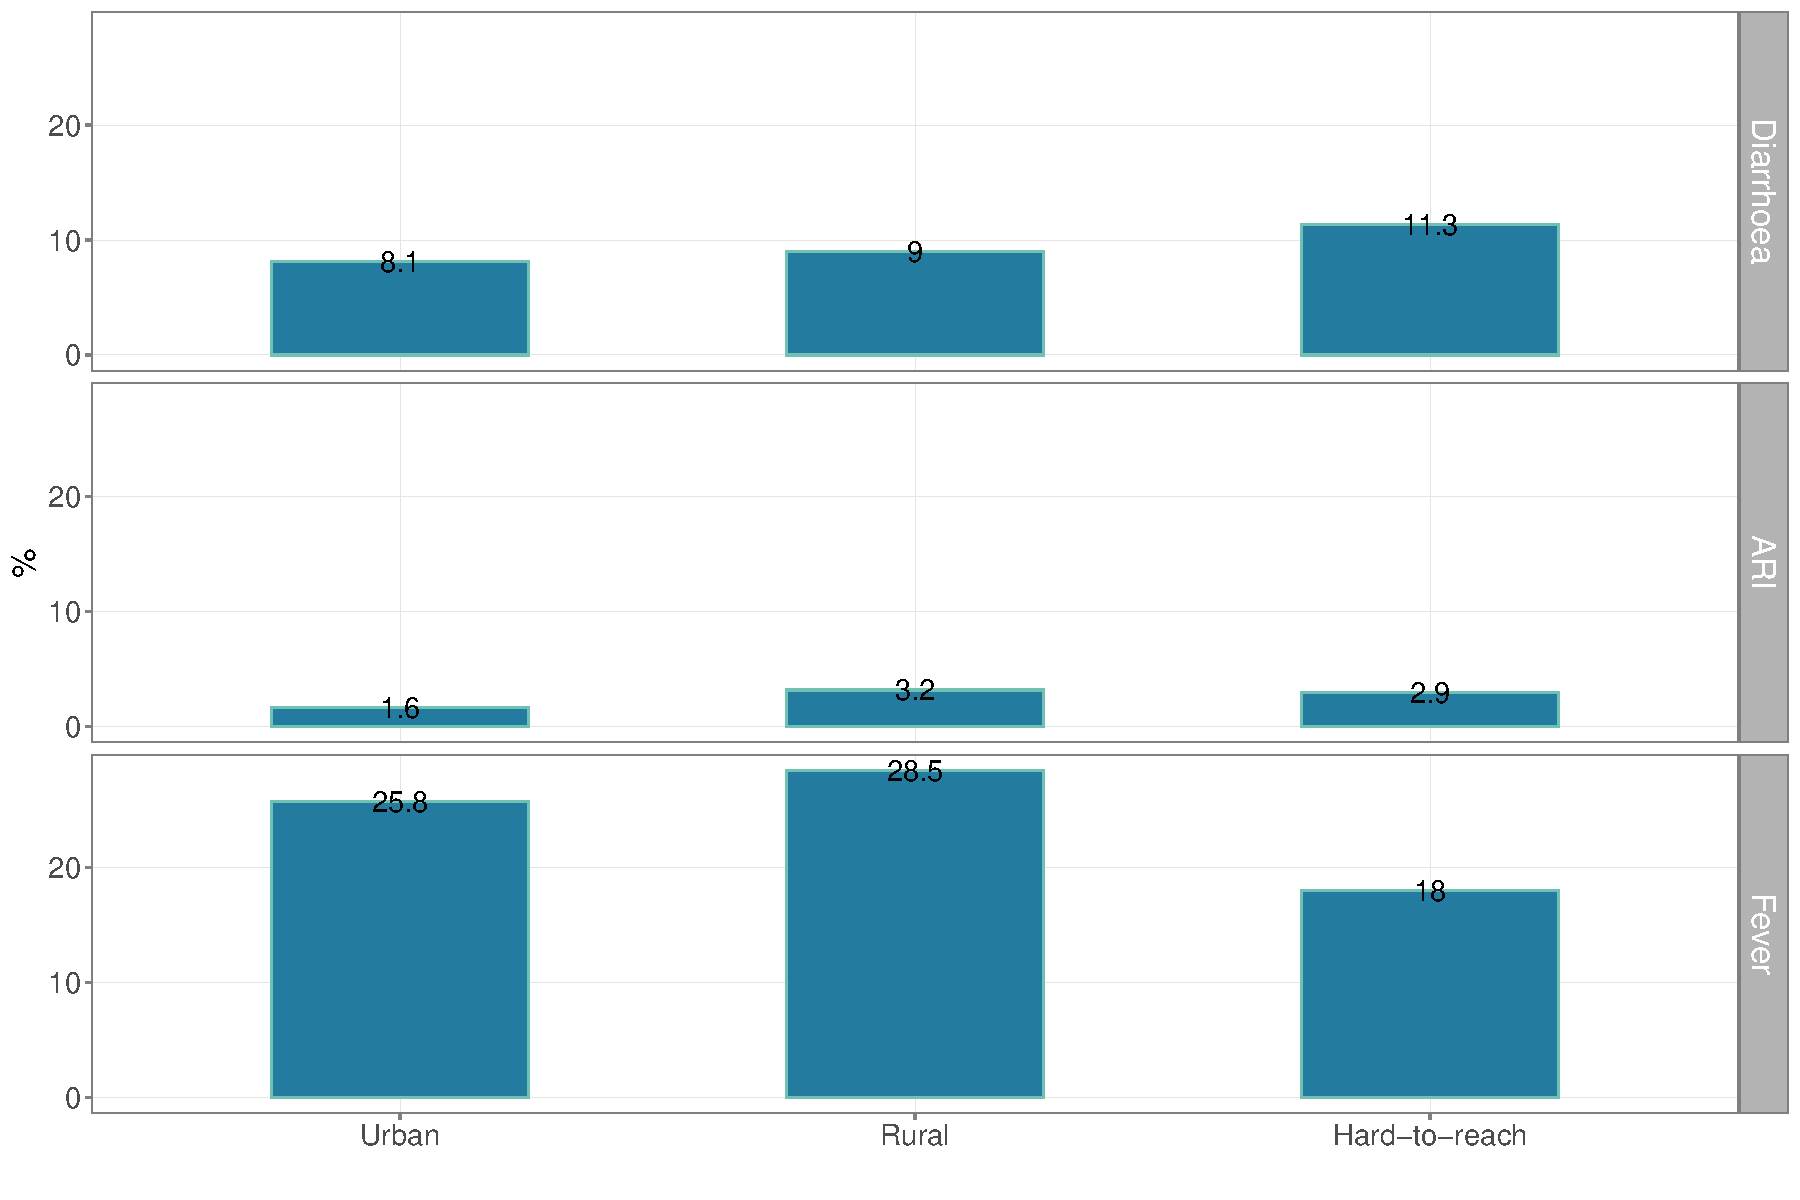
\includegraphics{kayinReport_files/figure-latex/ill1plot-1} 

}

\caption{Period prevalence of childhood illnesses by location type}\label{fig:ill1plot}
\end{figure}

\begin{figure}[H]

{\centering 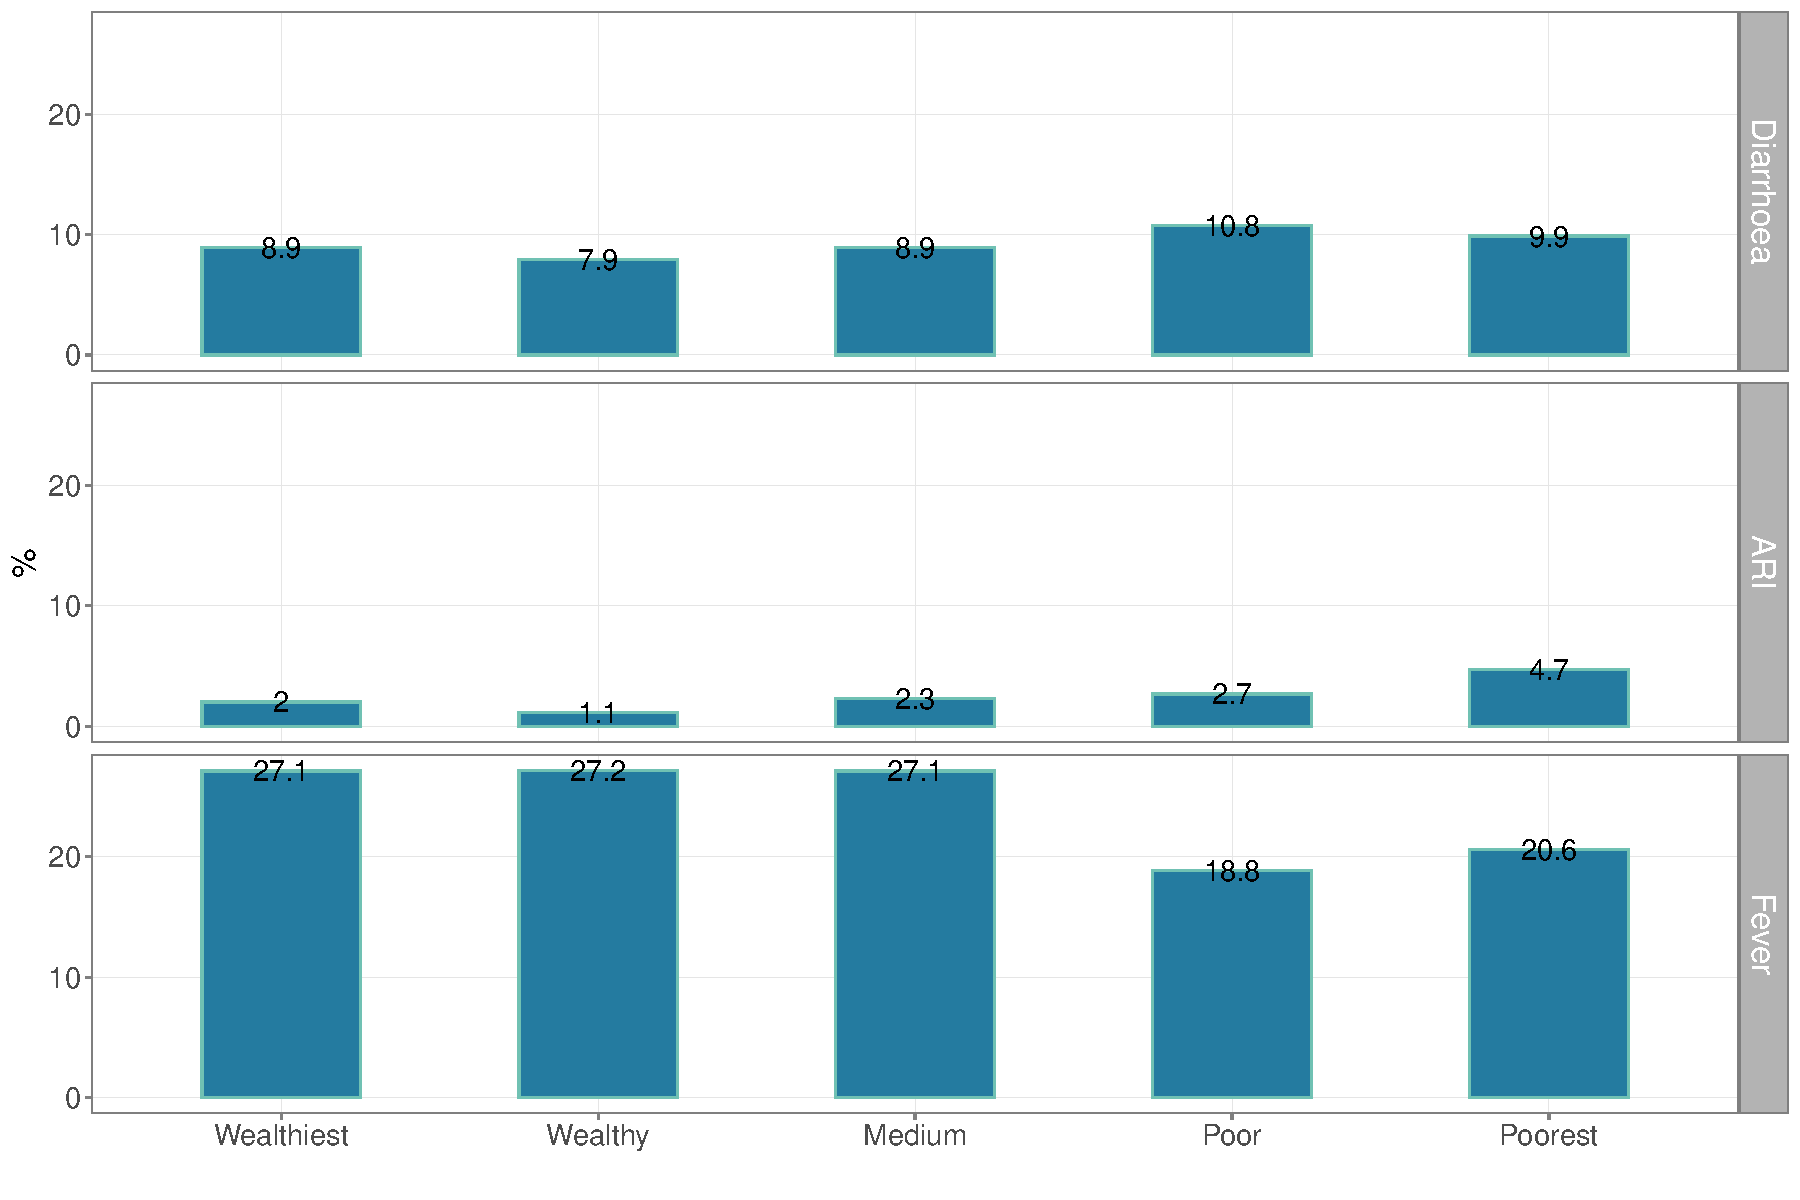
\includegraphics{kayinReport_files/figure-latex/ill2plot-1} 

}

\caption{Period prevalence of childhood illnesses by wealth quintiles}\label{fig:ill2plot}
\end{figure}

\hypertarget{ctreatment}{%
\paragraph{Treatment-seeking behaviour}\label{ctreatment}}

\hypertarget{diarrhoea}{%
\subparagraph{Diarrhoea}\label{diarrhoea}}

Treatment-seeking for diarrhoea in Kayin state can be characterised by households in urban areas seeking treatment the most (88\%) followed closely by those in hard-to-reach areas at 80\%. Those in urban areas are seeking treatment slightly less (see Figure \ref{fig:diarrhoea1plot}). Most households across the wealth classifications seek treatment for diarrhoea except for the poorest households who seek treatment for diarrhoea the least at 55\% and the wealthiest at 80\% (see Figure \ref{fig:diarrhoea2plot}). When asked why treatment was not sought for diarrhoea, those from the urban areas felt that treatment wasn't necessary and that cost was also a consideration whilst those in rural areas reported seeking alternative treatment and that health facility was inaccessible (see Figure \ref{fig:diarrhoea3plot}). Cost was the main reason for not seeking treatment from those in hard-to-reach areas. Time to treatment was short (1 day on average) and the same across areas (see Table \ref{tab:diarrhoea1table}).

Those from urban areas tended to see a private doctor whilst those from rural areas sought care from the RHC or the SRHC. Those from hard-to-reach areas tended to self-medicate or get care from an EHO clinic (see Figure \ref{fig:diarrhoea5plot}). Most of the wealthiest households sought treatment from a private clinic/doctor whilst the poor and the poorest households sought care from either the station hospital, ethnic health worker, community health worker or self-medicated with drugs from the shop (see Figure \ref{fig:diarrhoea6plot})

Costs incurred for treatment were mostly for medications (see Table \ref{tab:diarrhoea3table}).

\begin{landscape}\begin{table}[H]

\caption{\label{tab:diarrhoea1table}Treatment-seeking for diarrhoea}
\centering
\fontsize{10}{12}\selectfont
\begin{tabular}[t]{>{\bfseries}l>{\bfseries}l>{\ttfamily}r>{\ttfamily}r>{\ttfamily}r>{\ttfamily}r>{\ttfamily}r>{\ttfamily}r>{\ttfamily}r>{\ttfamily}r>{\ttfamily}r}
\toprule
\multicolumn{4}{c}{\textbf{ }} & \multicolumn{7}{c}{\textbf{Reasons for not seeking treatment}} \\
\cmidrule(l{3pt}r{3pt}){5-11}
 &  & \makecell[c]{Sought\\treatment\\(\%)} & \makecell[c]{Time to\\treatment\\(days)} & \makecell[c]{No\\facility\\(\%)} & \makecell[c]{Facility\\inaccessible\\(\%)} & \makecell[c]{Expensive\\(\%)} & \makecell[c]{Not\\necessary\\(\%)} & \makecell[c]{Advised\\not to\\(\%)} & \makecell[c]{Alternative\\treatment\\(\%)} & \makecell[c]{Do not know\\treamtent\\(\%)}\\
\midrule
\addlinespace[0.3em]
\multicolumn{11}{l}{\textbf{Kayin}}\\
\addlinespace[0.3em]
\multicolumn{11}{l}{\textit{\textbf{Geographic}}}\\
\hspace{1em}\hspace{1em} & Rural & 76.9 & 1.2 & 0 & 14.3 & 0.0 & 0.0 & 0 & 42.9 & 0\\
\cmidrule{2-11}
\hspace{1em}\hspace{1em} & Urban & 87.5 & 1.1 & 0 & 0.0 & 33.3 & 33.3 & 0 & 0.0 & 0\\
\cmidrule{2-11}
\hspace{1em}\hspace{1em} & Hard-to-reach & 80.0 & 1.3 & 0 & 0.0 & 50.0 & 0.0 & 0 & 0.0 & 0\\
\cmidrule{2-11}
\addlinespace[0.3em]
\multicolumn{11}{l}{\textit{\textbf{Wealth}}}\\
\hspace{1em}\hspace{1em} & Wealthiest & 80.0 & 1.0 & 0 & 0.0 & 50.0 & 0.0 & 0 & 0.0 & 0\\
\cmidrule{2-11}
\hspace{1em}\hspace{1em} & Wealthy & 100.0 & 1.3 & 0 & 0.0 & 0.0 & 0.0 & 0 & 0.0 & 0\\
\cmidrule{2-11}
\hspace{1em}\hspace{1em} & Medium & 100.0 & 1.2 & 0 & 0.0 & 0.0 & 0.0 & 0 & 0.0 & 0\\
\cmidrule{2-11}
\hspace{1em}\hspace{1em} & Poor & 100.0 & 1.3 & 0 & 0.0 & 0.0 & 0.0 & 0 & 100.0 & 0\\
\cmidrule{2-11}
\hspace{1em}\hspace{1em} & Poorest & 54.5 & 1.3 & 0 & 10.0 & 30.0 & 10.0 & 0 & 10.0 & 0\\
\bottomrule
\end{tabular}
\end{table}
\end{landscape}

\begin{figure}[H]

{\centering 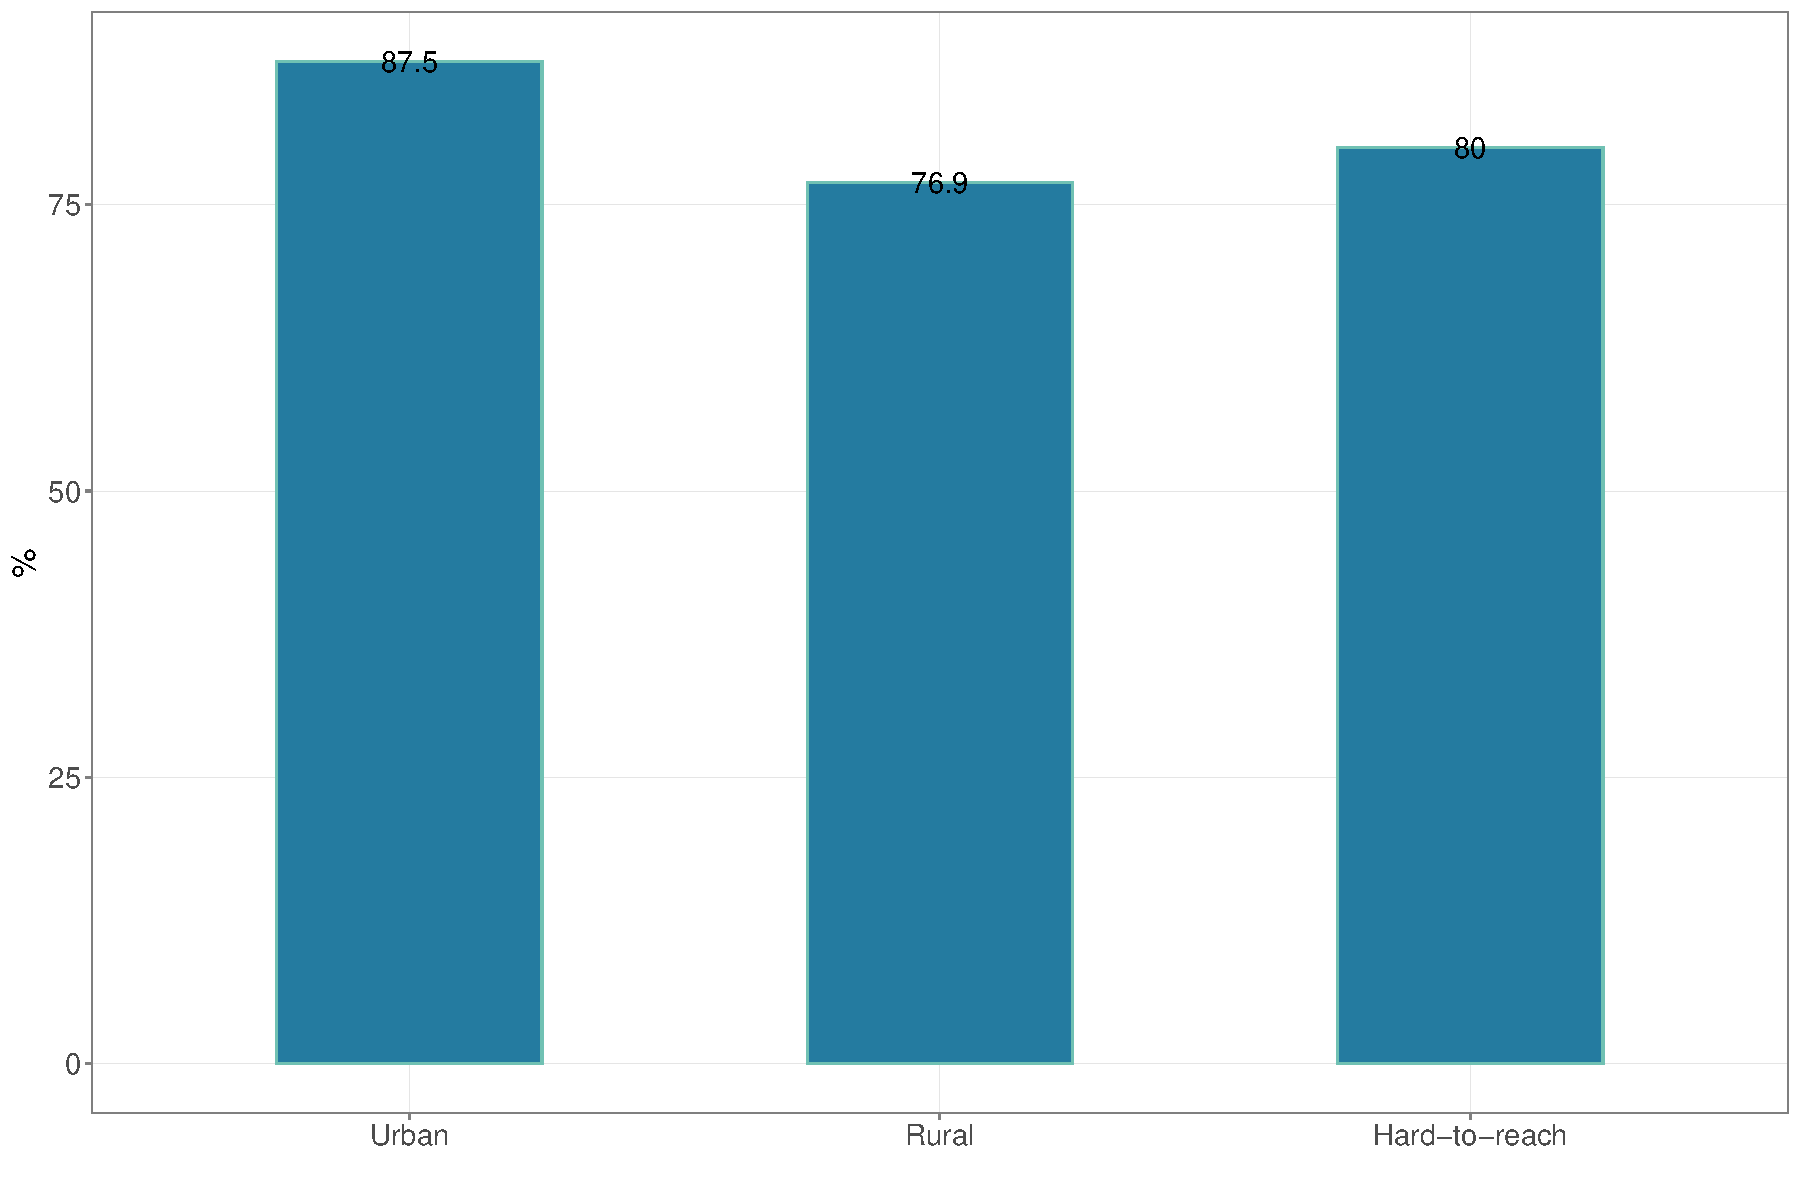
\includegraphics{kayinReport_files/figure-latex/diarrhoea1plot-1} 

}

\caption{Treatment-seeking for diarrhoea by location type}\label{fig:diarrhoea1plot}
\end{figure}

\begin{figure}[H]

{\centering 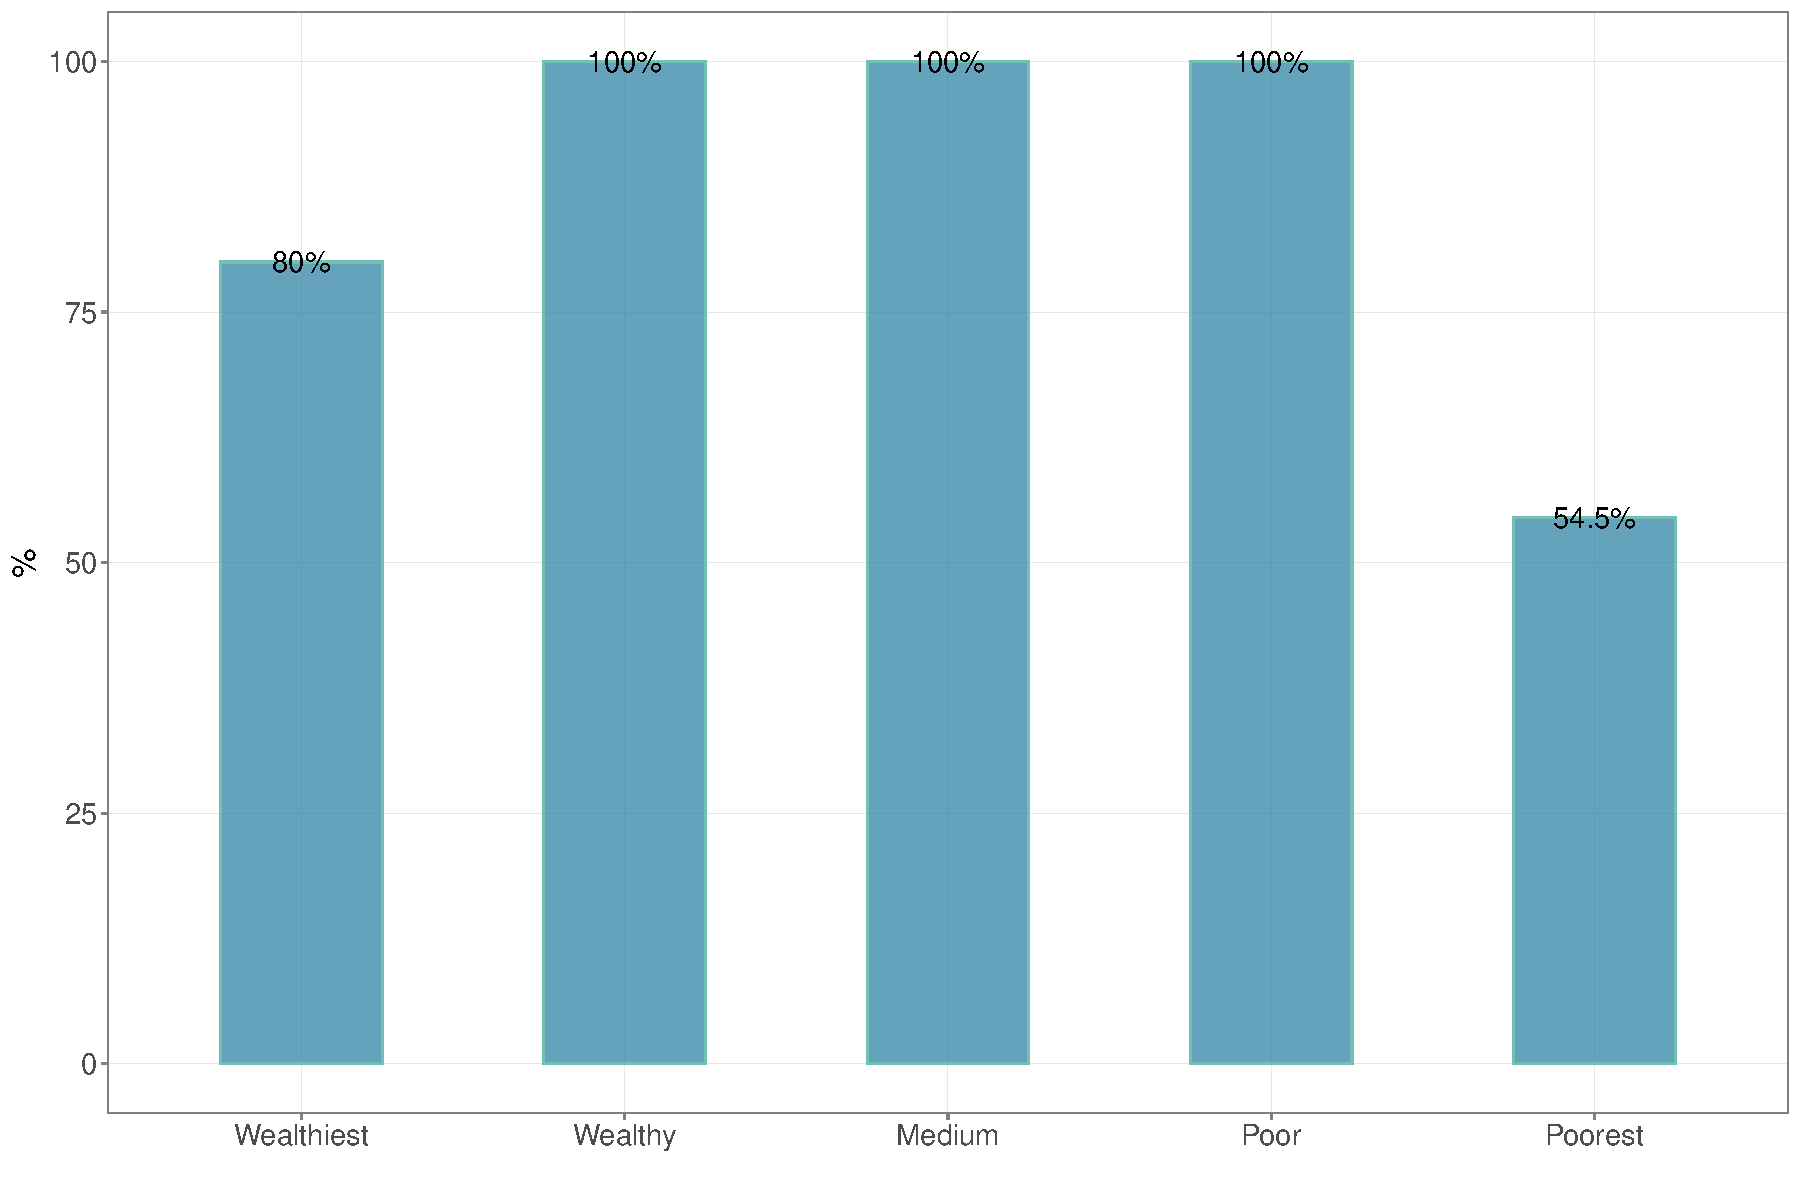
\includegraphics{kayinReport_files/figure-latex/diarrhoea2plot-1} 

}

\caption{Treatment-seeking for diarrhoea by wealth quintiles}\label{fig:diarrhoea2plot}
\end{figure}

\begin{figure}[H]

{\centering 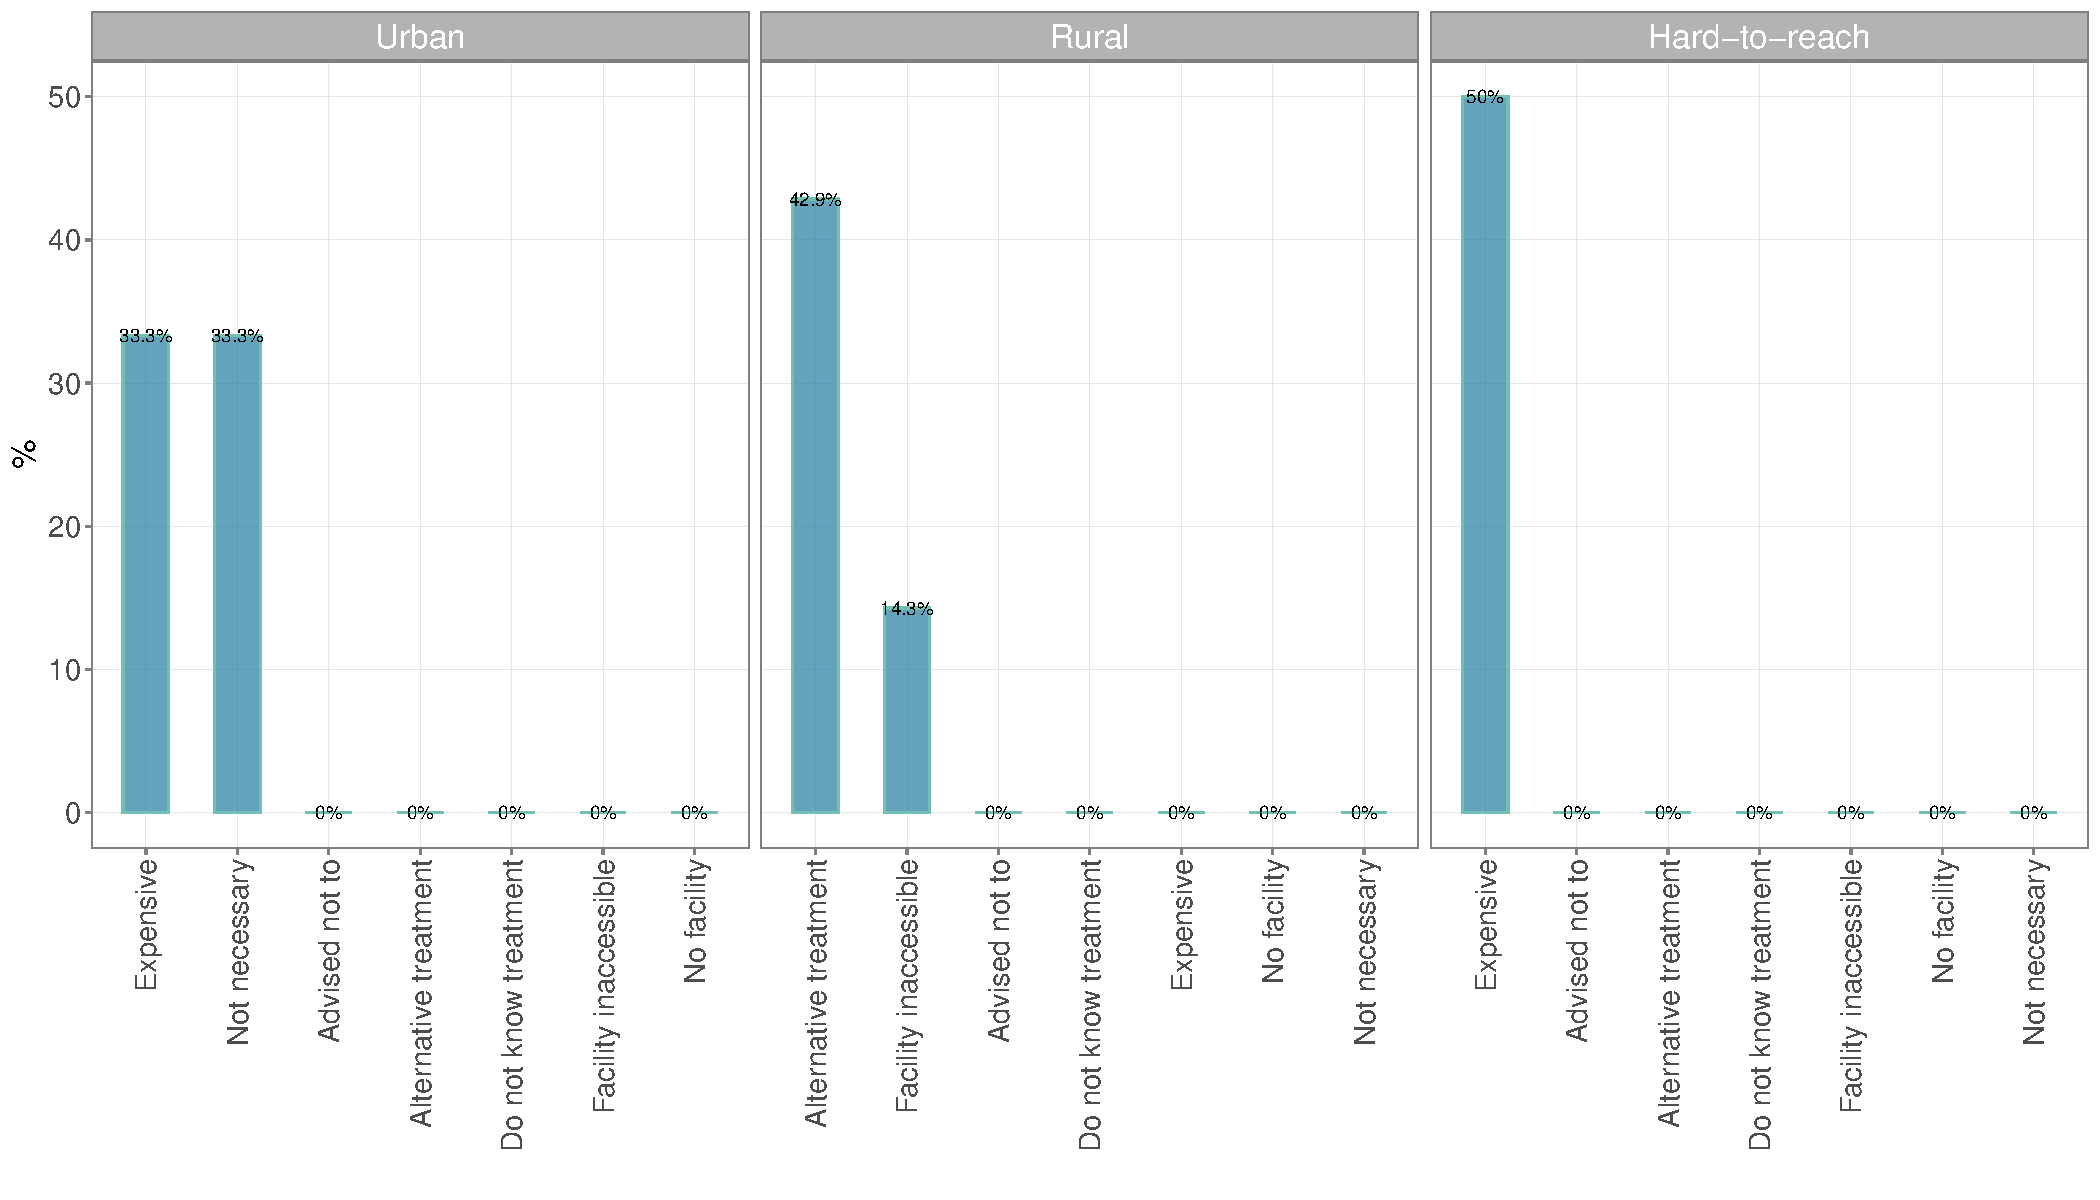
\includegraphics{kayinReport_files/figure-latex/diarrhoea3plot-1} 

}

\caption{Reasons for not seeking treatment by location type}\label{fig:diarrhoea3plot}
\end{figure}

\begin{figure}[H]

{\centering 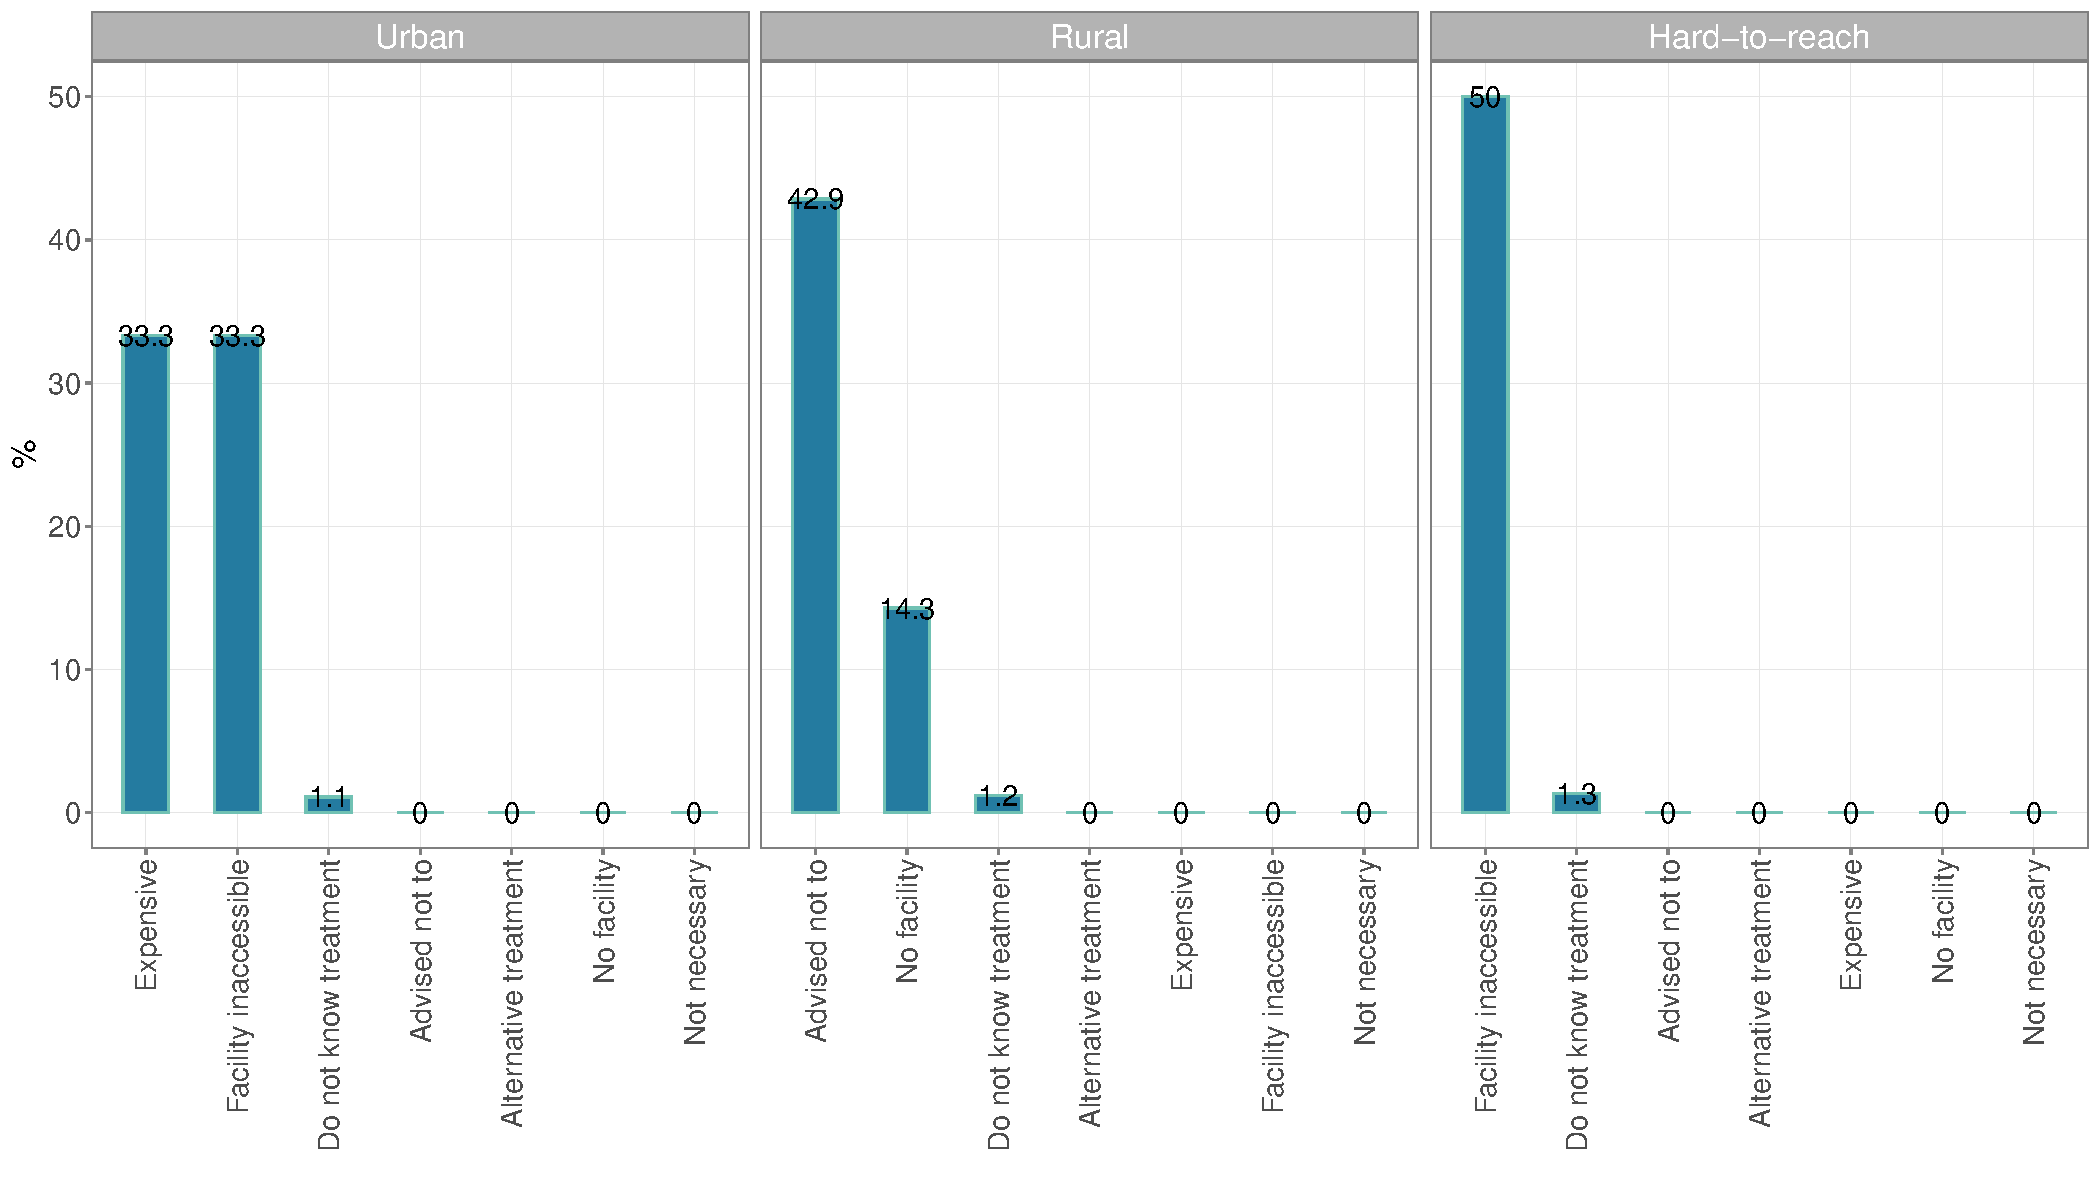
\includegraphics{kayinReport_files/figure-latex/diarrhoea4plot-1} 

}

\caption{Reasons for not seeking treatment by wealth quintiles}\label{fig:diarrhoea4plot}
\end{figure}

\begin{landscape}\begin{table}[H]

\caption{\label{tab:diarrhoea2table}Where/who treatment is sought from}
\centering
\fontsize{9}{11}\selectfont
\begin{tabular}[t]{>{\bfseries}l>{\bfseries}l>{\ttfamily}r>{\ttfamily}r>{\ttfamily}r>{\ttfamily}r>{\ttfamily}r>{\ttfamily}r>{\ttfamily}r>{\ttfamily}r>{\ttfamily}r>{\ttfamily}r>{\ttfamily}r>{\ttfamily}r>{\ttfamily}r}
\toprule
\multicolumn{2}{c}{\textbf{ }} & \multicolumn{13}{c}{\textbf{Where/who treatment is sought from}} \\
\cmidrule(l{3pt}r{3pt}){3-15}
 &  & \makecell[c]{Township\\hospital\\(\%)} & \makecell[c]{Station\\hospital\\(\%)} & \makecell[c]{RHC/\\health\\assistant\\(\%)} & \makecell[c]{SRHC/\\midwife\\(\%)} & \makecell[c]{Private\\clinic/\\doctor\\(\%)} & \makecell[c]{Community\\health\\worker\\(\%)} & \makecell[c]{Traditional\\healer\\(\%)} & \makecell[c]{Untrained\\health\\worker\\(\%)} & \makecell[c]{Drug\\from\\shop\\(\%)} & \makecell[c]{EHO\\clinic/\\volunteer\\(\%)} & \makecell[c]{Family\\member\\(\%)} & \makecell[c]{NGOs/\\clinic\\(\%)} & \makecell[c]{Auxilliary\\midwife\\(\%)}\\
\midrule
\addlinespace[0.3em]
\multicolumn{15}{l}{\textbf{Kayin}}\\
\addlinespace[0.3em]
\multicolumn{15}{l}{\textit{\textbf{Geographic}}}\\
\hspace{1em}\hspace{1em} & Rural & 11.1 & 5.6 & 22.2 & 22.2 & 0.0 & 5.6 & 0.0 & 0.0 & 11.1 & 0.0 & 0.0 & 0 & 11.1\\
\cmidrule{2-15}
\hspace{1em}\hspace{1em} & Urban & 9.1 & 0.0 & 0.0 & 9.1 & 81.8 & 0.0 & 0.0 & 0.0 & 0.0 & 0.0 & 0.0 & 0 & 0.0\\
\cmidrule{2-15}
\hspace{1em}\hspace{1em} & Hard-to-reach & 0.0 & 13.0 & 4.3 & 8.7 & 4.3 & 8.7 & 4.3 & 4.3 & 21.7 & 21.7 & 8.7 & 0 & 0.0\\
\cmidrule{2-15}
\addlinespace[0.3em]
\multicolumn{15}{l}{\textit{\textbf{Wealth}}}\\
\hspace{1em}\hspace{1em} & Wealthiest & 0.0 & 0.0 & 0.0 & 14.3 & 85.7 & 0.0 & 0.0 & 0.0 & 0.0 & 0.0 & 0.0 & 0 & 0.0\\
\cmidrule{2-15}
\hspace{1em}\hspace{1em} & Wealthy & 0.0 & 16.7 & 16.7 & 0.0 & 33.3 & 0.0 & 0.0 & 0.0 & 0.0 & 0.0 & 16.7 & 0 & 0.0\\
\cmidrule{2-15}
\hspace{1em}\hspace{1em} & Medium & 8.3 & 0.0 & 0.0 & 33.3 & 0.0 & 8.3 & 0.0 & 8.3 & 25.0 & 0.0 & 8.3 & 0 & 0.0\\
\cmidrule{2-15}
\hspace{1em}\hspace{1em} & Poor & 7.7 & 15.4 & 23.1 & 7.7 & 7.7 & 0.0 & 7.7 & 0.0 & 7.7 & 15.4 & 0.0 & 0 & 7.7\\
\cmidrule{2-15}
\hspace{1em}\hspace{1em} & Poorest & 0.0 & 7.7 & 7.7 & 7.7 & 7.7 & 15.4 & 0.0 & 0.0 & 23.1 & 23.1 & 0.0 & 0 & 7.7\\
\bottomrule
\end{tabular}
\end{table}
\end{landscape}

\begin{figure}[H]

{\centering 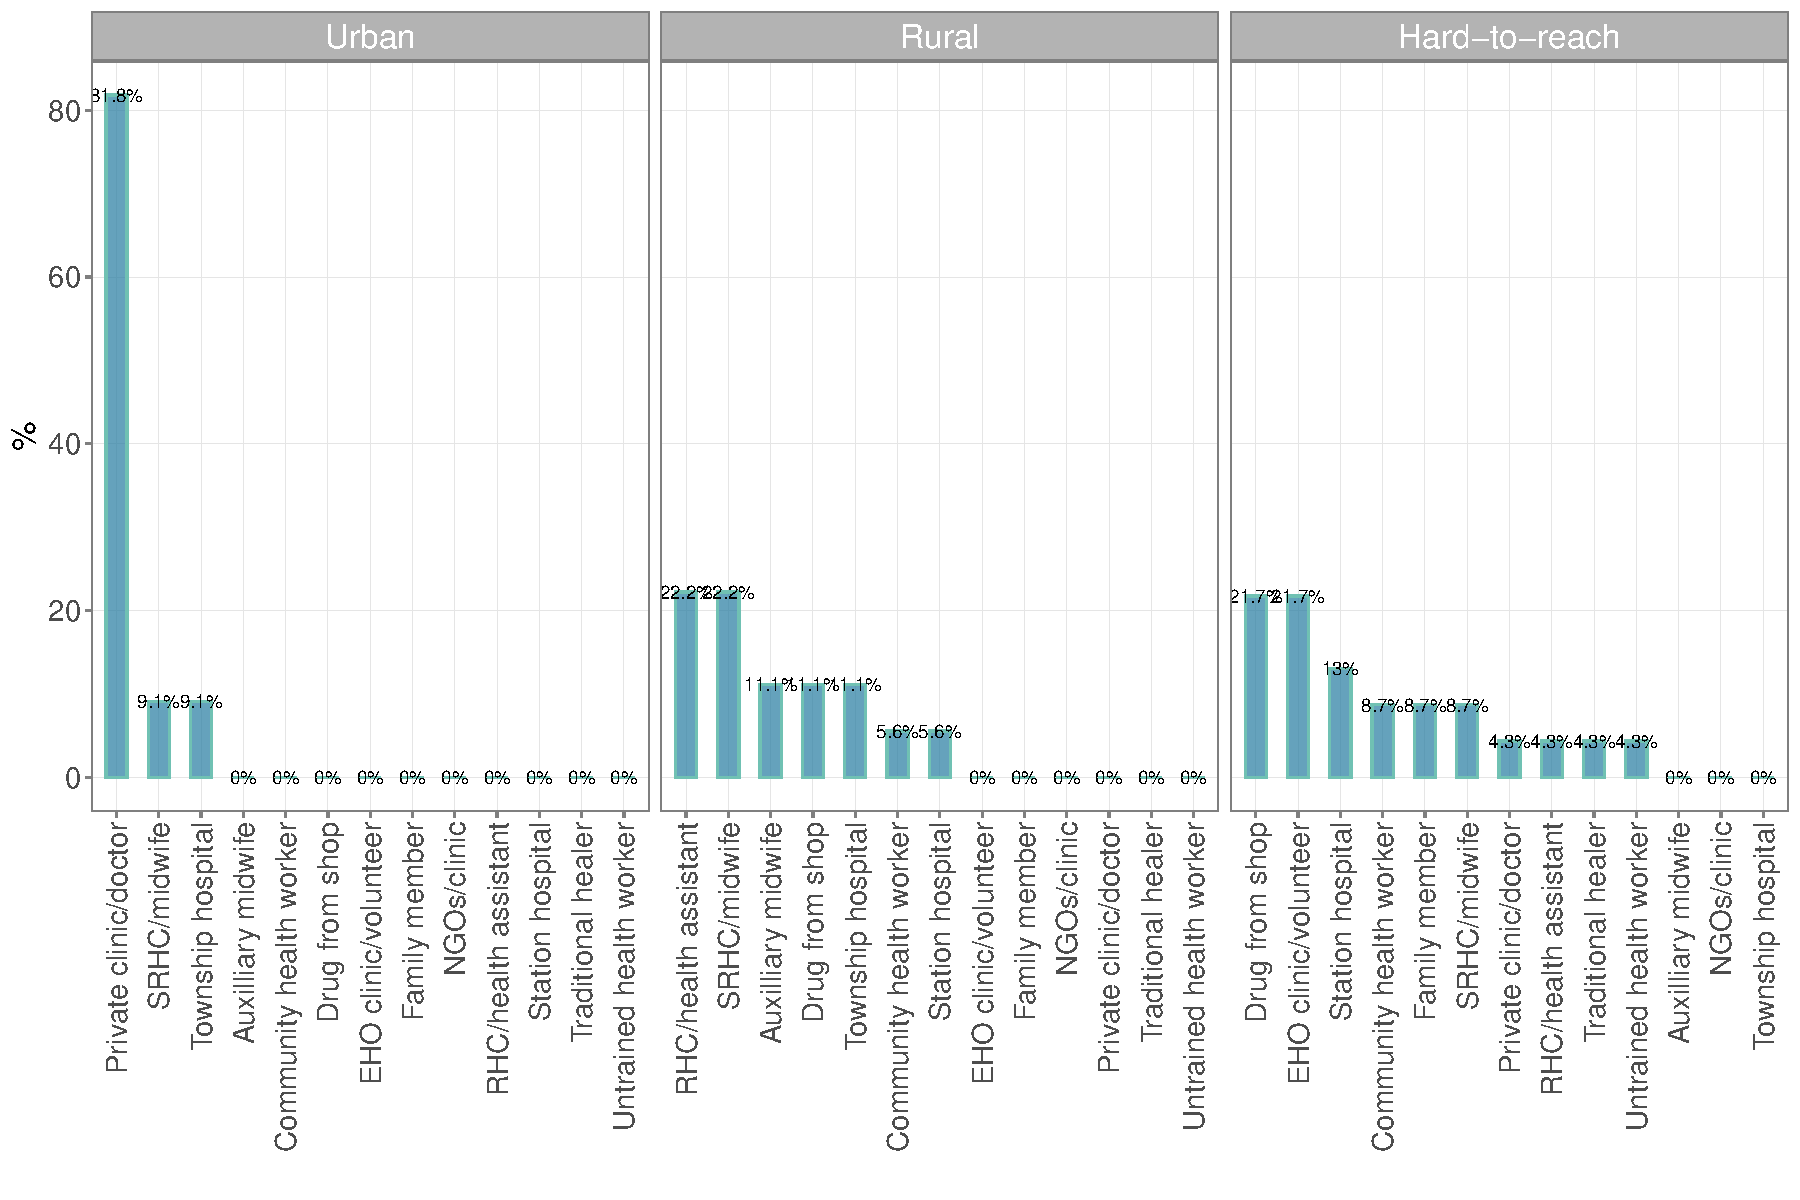
\includegraphics{kayinReport_files/figure-latex/diarrhoea5plot-1} 

}

\caption{Where/who treatment is sought from by location type}\label{fig:diarrhoea5plot}
\end{figure}

\begin{figure}[H]

{\centering 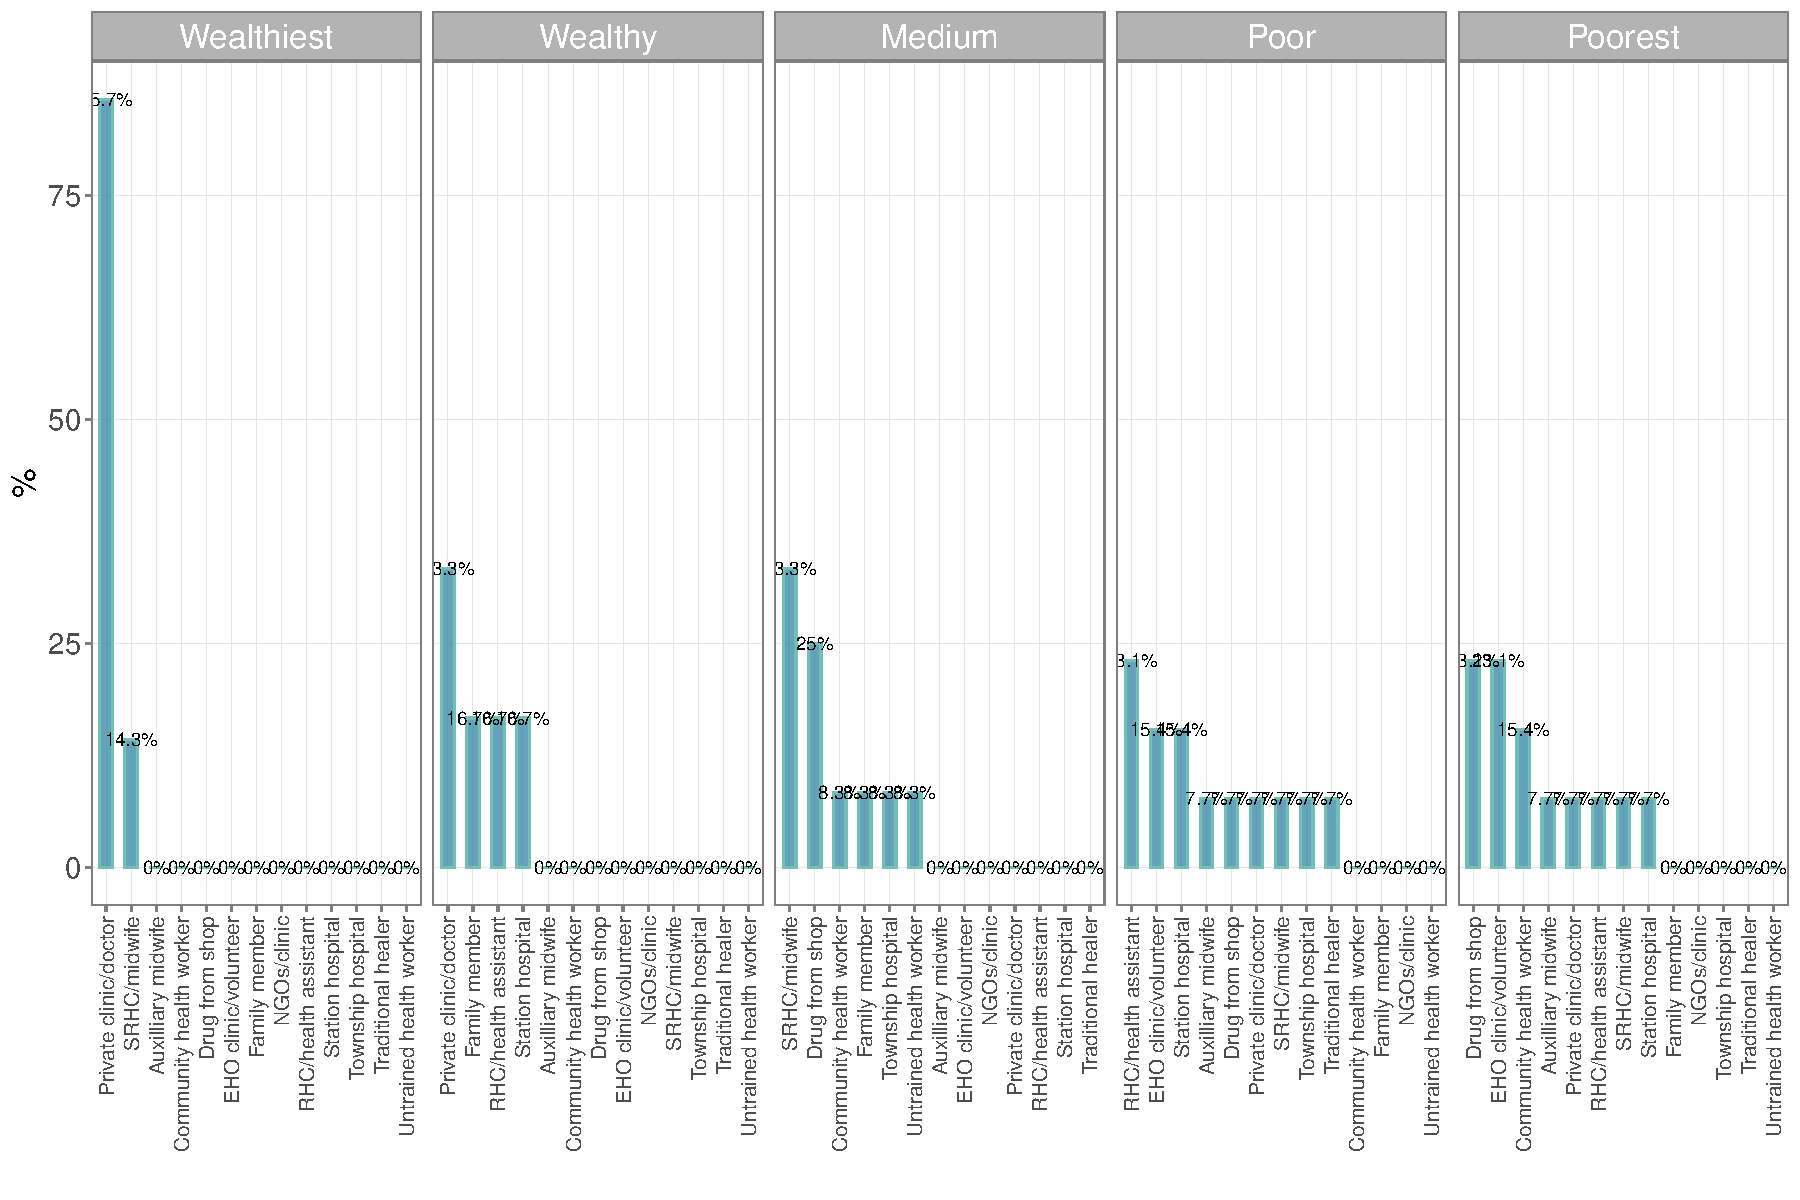
\includegraphics{kayinReport_files/figure-latex/diarrhoea6plot-1} 

}

\caption{Where/who treatment is sought from by wealth quintiles}\label{fig:diarrhoea6plot}
\end{figure}

\begin{landscape}\begin{table}[H]

\caption{\label{tab:diarrhoea3table}Payment for treatment}
\centering
\fontsize{10}{12}\selectfont
\begin{tabular}[t]{>{\bfseries}l>{\bfseries}l>{\ttfamily}r>{\ttfamily}r>{\ttfamily}r>{\ttfamily}r>{\ttfamily}r>{\ttfamily}r>{\ttfamily}r>{\ttfamily}r}
\toprule
\multicolumn{3}{c}{\textbf{ }} & \multicolumn{6}{c}{\textbf{Payment for}} & \multicolumn{1}{c}{\textbf{ }} \\
\cmidrule(l{3pt}r{3pt}){4-9}
 &  & \makecell[c]{Payment\\for\\service\\(MMK)} & \makecell[c]{Transportation\\(\%)} & \makecell[c]{Registration\\(\%)} & \makecell[c]{Medicine\\(\%)} & \makecell[c]{Laboratory\\fees\\(\%)} & \makecell[c]{Provider\\fees\\(\%)} & \makecell[c]{Gifts\\(\%)} & \makecell[c]{Took\\loan\\(\%)}\\
\midrule
\addlinespace[0.3em]
\multicolumn{10}{l}{\textbf{Kayin}}\\
\addlinespace[0.3em]
\multicolumn{10}{l}{\textit{\textbf{Geographic}}}\\
\hspace{1em}\hspace{1em} & Rural & 13700.5 & 0.0 & 0 & 100.0 & 0 & 0 & 0 & 18.8\\
\cmidrule{2-10}
\hspace{1em}\hspace{1em} & Urban & 7681.8 & 0.0 & 0 & 100.0 & 0 & 0 & 0 & 20.0\\
\cmidrule{2-10}
\hspace{1em}\hspace{1em} & Hard-to-reach & 6869.6 & 6.7 & 0 & 86.7 & 0 & 0 & 0 & 15.8\\
\cmidrule{2-10}
\addlinespace[0.3em]
\multicolumn{10}{l}{\textit{\textbf{Wealth}}}\\
\hspace{1em}\hspace{1em} & Wealthiest & 8214.3 & 0.0 & 0 & 100.0 & 0 & 0 & 0 & 16.7\\
\cmidrule{2-10}
\hspace{1em}\hspace{1em} & Wealthy & 8333.3 & 0.0 & 0 & 100.0 & 0 & 0 & 0 & 20.0\\
\cmidrule{2-10}
\hspace{1em}\hspace{1em} & Medium & 7909.1 & 0.0 & 0 & 100.0 & 0 & 0 & 0 & 27.3\\
\cmidrule{2-10}
\hspace{1em}\hspace{1em} & Poor & 2625.7 & 0.0 & 0 & 100.0 & 0 & 0 & 0 & 18.2\\
\cmidrule{2-10}
\hspace{1em}\hspace{1em} & Poorest & 17207.7 & 11.1 & 0 & 77.8 & 0 & 0 & 0 & 9.1\\
\bottomrule
\end{tabular}
\end{table}
\end{landscape}

\begin{figure}[H]

{\centering 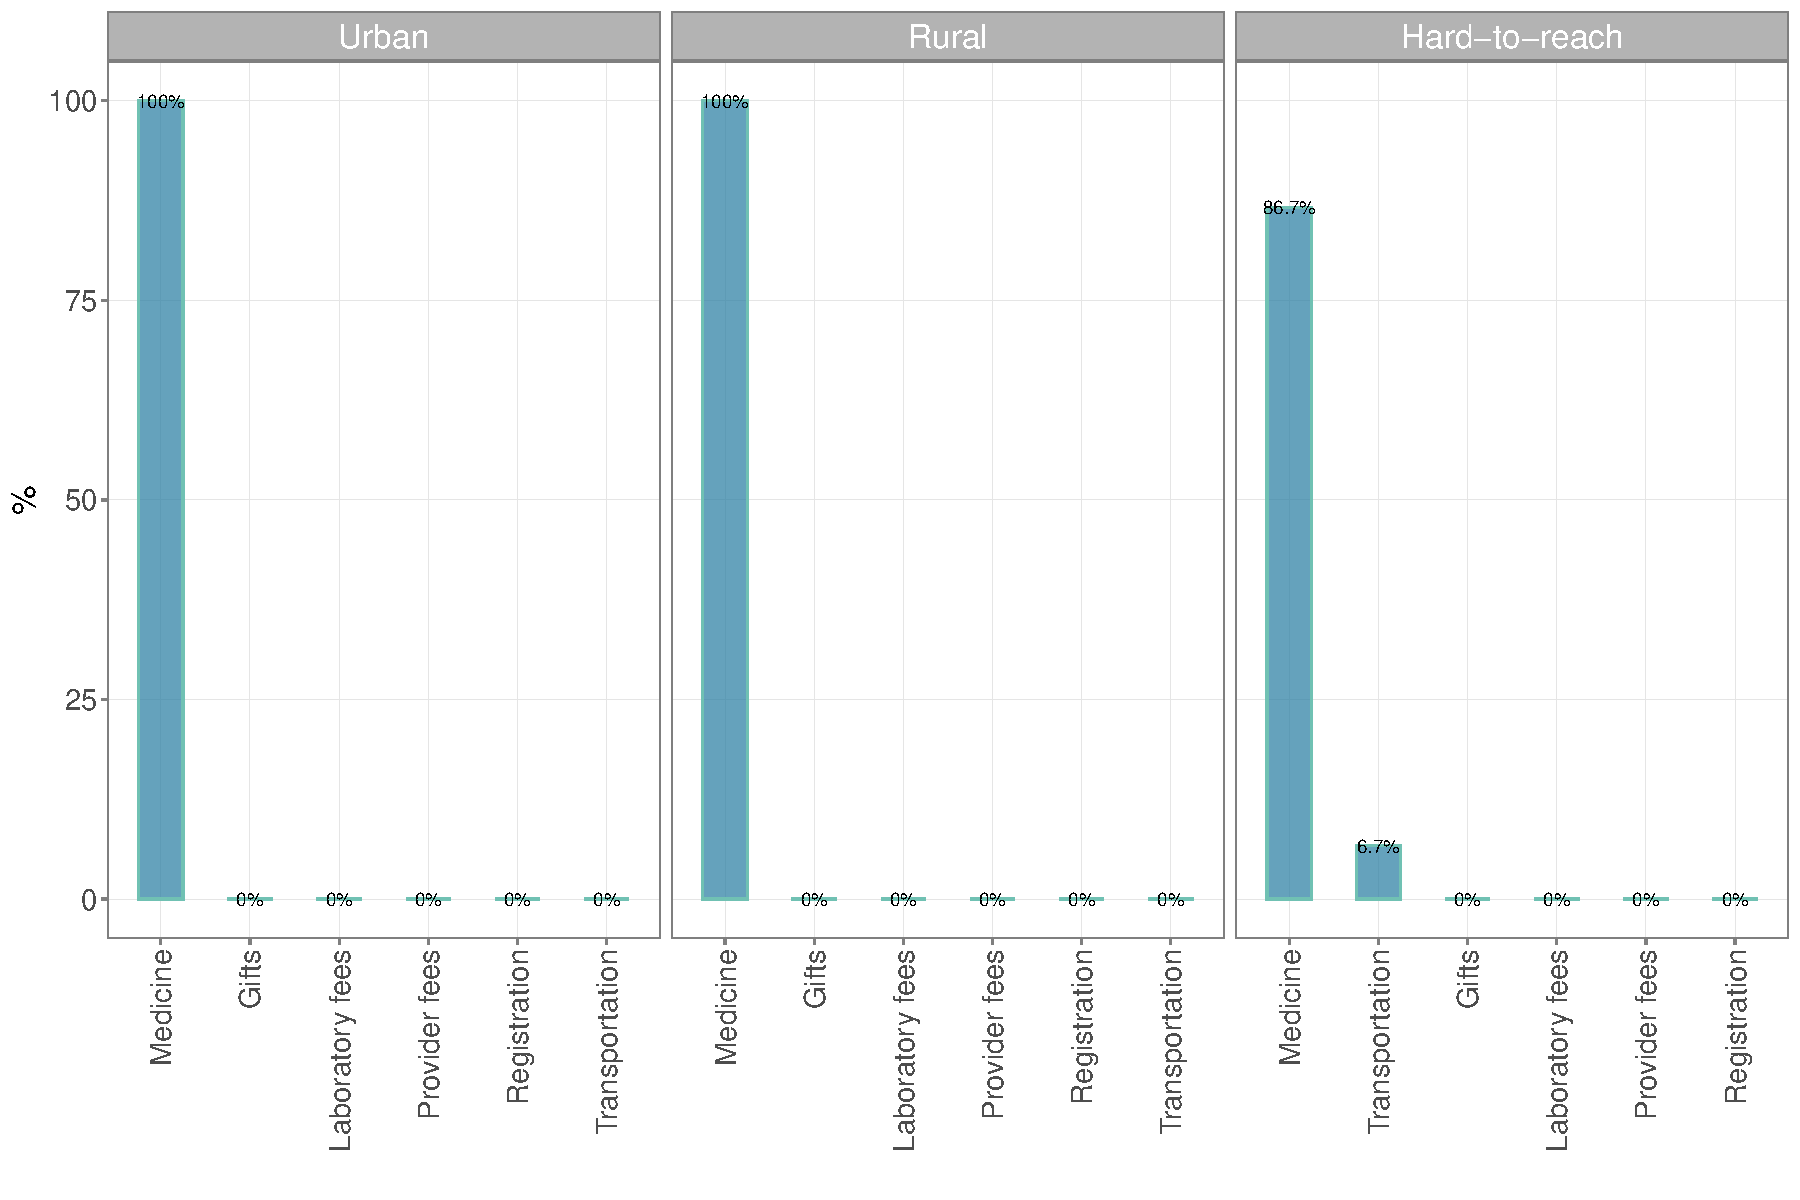
\includegraphics{kayinReport_files/figure-latex/diarrhoea7plot-1} 

}

\caption{Costs incurred for treatment by location type}\label{fig:diarrhoea7plot}
\end{figure}

\begin{figure}[H]

{\centering 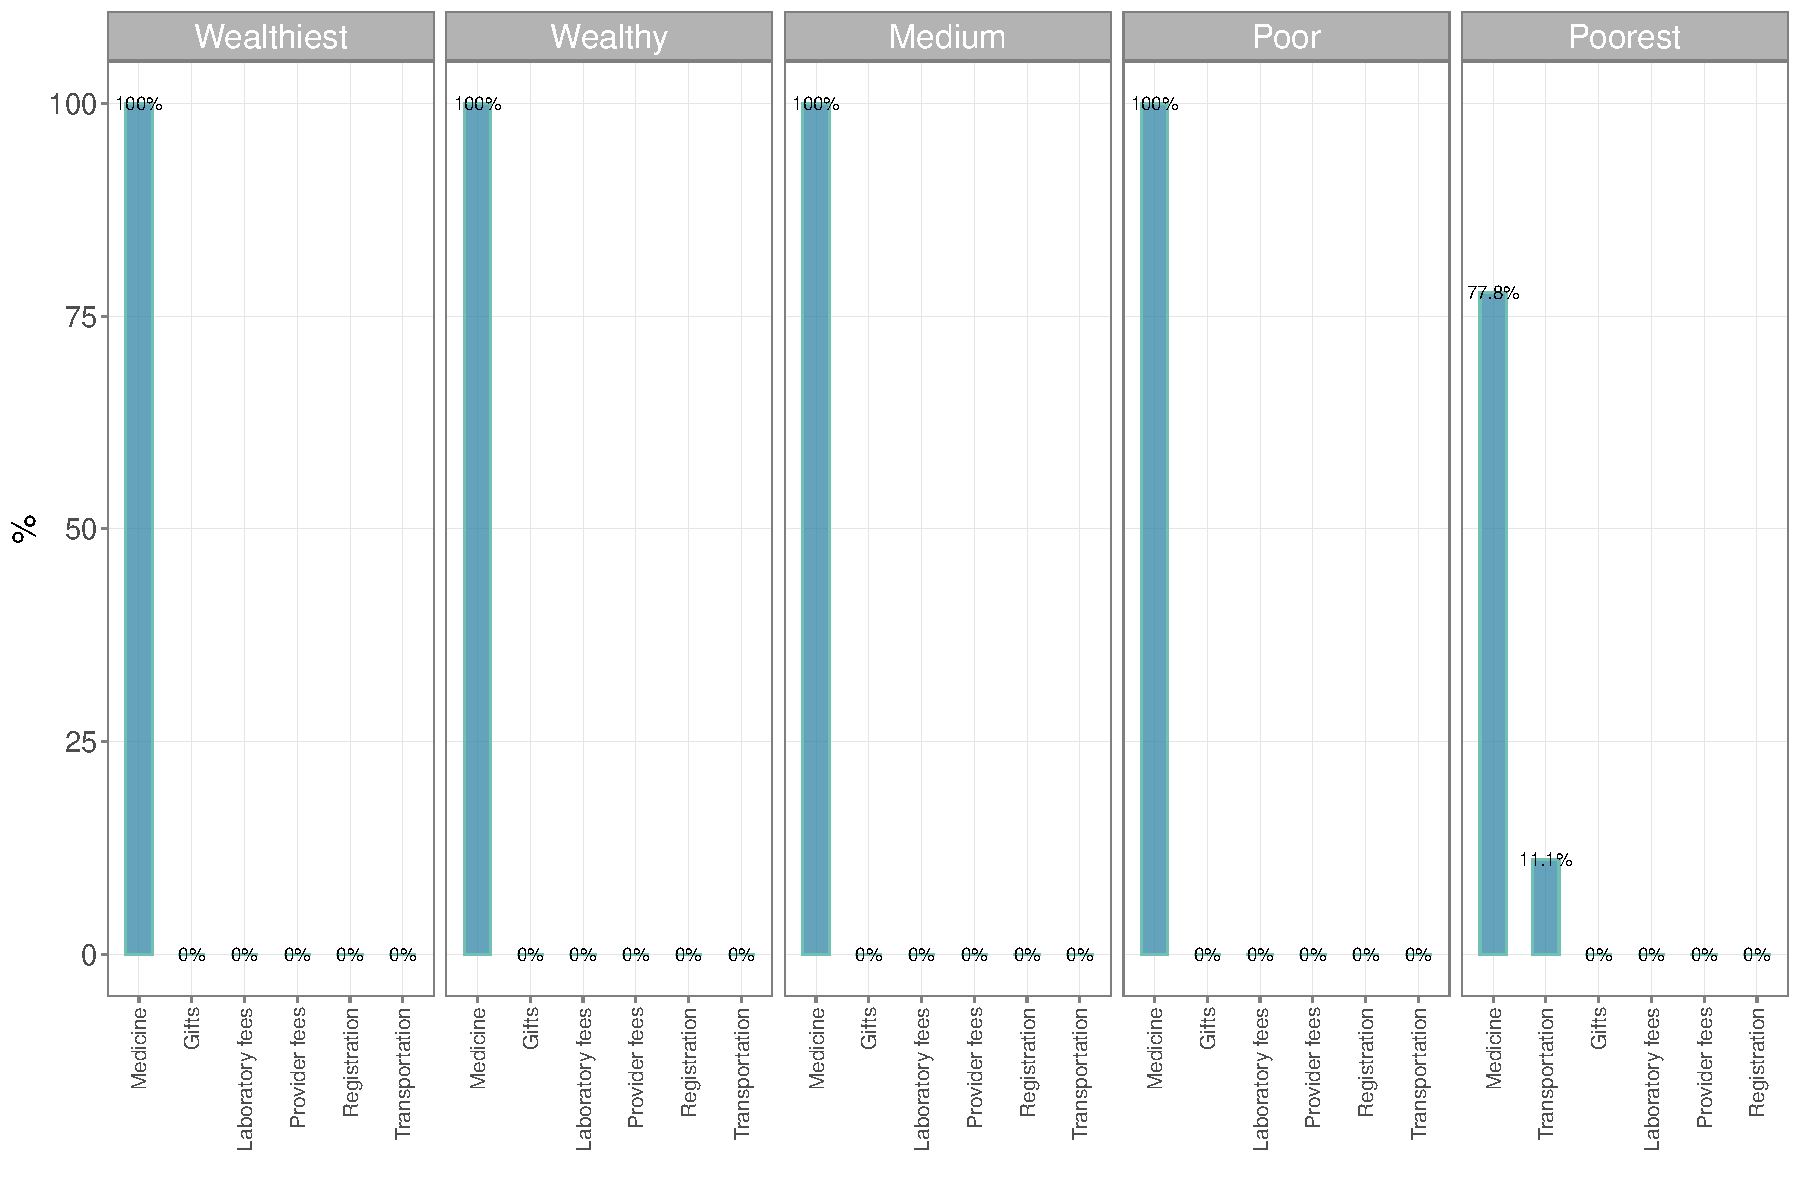
\includegraphics{kayinReport_files/figure-latex/diarrhoea8plot-1} 

}

\caption{Costs incurred for treatment by wealth quintile}\label{fig:diarrhoea8plot}
\end{figure}

\hypertarget{ari}{%
\subparagraph{Acute respiratory infection}\label{ari}}

Treatment-seeking for ARI in Kayin state can be characterised by households in rural areas seeking treatment the most (89.2\%) followed closely by those from urban areas at 85\% whilst those in hard-to-reach areas seeking treatment less at 74\% (see Figure \ref{fig:ari1plot}). Most households in the wealthier classes and much lesser number of households from the poorer classes sought care for ARI (see Figure \ref{fig:ari2plot}).

When asked why treatment was not sought for ARI, those from the urban areas didn't think it was necessary or found alternative treatment. Those from hard-to-reach areas, on the other hand, don't know treatment for ARI hence have not sough care (see Figure \ref{fig:ari3plot}). Amongst the wealthier households, most think that treatment wasn't necessary or sought alternative treatment. Those in the poorer households, on the other hand, don't know of any treatment whilst also thinking that treatment wasn't necessary or seeking alternative treatment (see Figure \ref{fig:ari4plot}).

Those from urban areas tended to see a private doctor whilst those from rural and hard-to-reach areas predominantly went to the EHO clinic or self-medicated (see Figure \ref{fig:ari5plot}). The wealthier households sought treatement for ARI from a private clinic/doctor whilst the poorer households went to the ethnic health worker or self-medicated (see Figure \ref{fig:ari6plot}).

Costs incurred for treatment were primarily for medications (see Table \ref{tab:ari3table}).

\begin{landscape}\begin{table}[H]

\caption{\label{tab:ari1table}Treatment-seeking for acute respiratory infection}
\centering
\fontsize{10}{12}\selectfont
\begin{tabular}[t]{>{\bfseries}l>{\bfseries}l>{\ttfamily}r>{\ttfamily}r>{\ttfamily}r>{\ttfamily}r>{\ttfamily}r>{\ttfamily}r>{\ttfamily}r>{\ttfamily}r>{\ttfamily}r}
\toprule
\multicolumn{4}{c}{\textbf{ }} & \multicolumn{7}{c}{\textbf{Reasons for not seeking treatment}} \\
\cmidrule(l{3pt}r{3pt}){5-11}
 &  & \makecell[c]{Sought\\treatment\\(\%)} & \makecell[c]{Time to\\treatment\\(days)} & \makecell[c]{No\\facility\\(\%)} & \makecell[c]{Facility\\inaccessible\\(\%)} & \makecell[c]{Expensive\\(\%)} & \makecell[c]{Not\\necessary\\(\%)} & \makecell[c]{Advised\\not to\\(\%)} & \makecell[c]{Alternative\\treatment\\(\%)} & \makecell[c]{Do not know\\treamtent\\(\%)}\\
\midrule
\addlinespace[0.3em]
\multicolumn{11}{l}{\textbf{Kayin}}\\
\addlinespace[0.3em]
\multicolumn{11}{l}{\textit{\textbf{Geographic}}}\\
\hspace{1em}\hspace{1em} & Rural & 89.2 & 1.4 & 0.0 & 11.1 & 0.0 & 0.0 & 0 & 11.1 & 0.0\\
\cmidrule{2-11}
\hspace{1em}\hspace{1em} & Urban & 85.0 & 1.3 & 0.0 & 0.0 & 0.0 & 30.0 & 0 & 30.0 & 0.0\\
\cmidrule{2-11}
\hspace{1em}\hspace{1em} & Hard-to-reach & 74.4 & 1.4 & 7.1 & 7.1 & 7.1 & 0.0 & 0 & 0.0 & 21.4\\
\cmidrule{2-11}
\addlinespace[0.3em]
\multicolumn{11}{l}{\textit{\textbf{Wealth}}}\\
\hspace{1em}\hspace{1em} & Wealthiest & 90.9 & 1.3 & 0.0 & 0.0 & 0.0 & 0.0 & 0 & 50.0 & 0.0\\
\cmidrule{2-11}
\hspace{1em}\hspace{1em} & Wealthy & 95.2 & 1.3 & 0.0 & 0.0 & 0.0 & 50.0 & 0 & 0.0 & 0.0\\
\cmidrule{2-11}
\hspace{1em}\hspace{1em} & Medium & 82.6 & 1.2 & 0.0 & 40.0 & 0.0 & 0.0 & 0 & 0.0 & 20.0\\
\cmidrule{2-11}
\hspace{1em}\hspace{1em} & Poor & 75.0 & 1.3 & 10.0 & 0.0 & 0.0 & 0.0 & 0 & 10.0 & 10.0\\
\cmidrule{2-11}
\hspace{1em}\hspace{1em} & Poorest & 73.9 & 1.8 & 0.0 & 0.0 & 9.1 & 18.2 & 0 & 0.0 & 9.1\\
\bottomrule
\end{tabular}
\end{table}
\end{landscape}

\begin{figure}[H]

{\centering 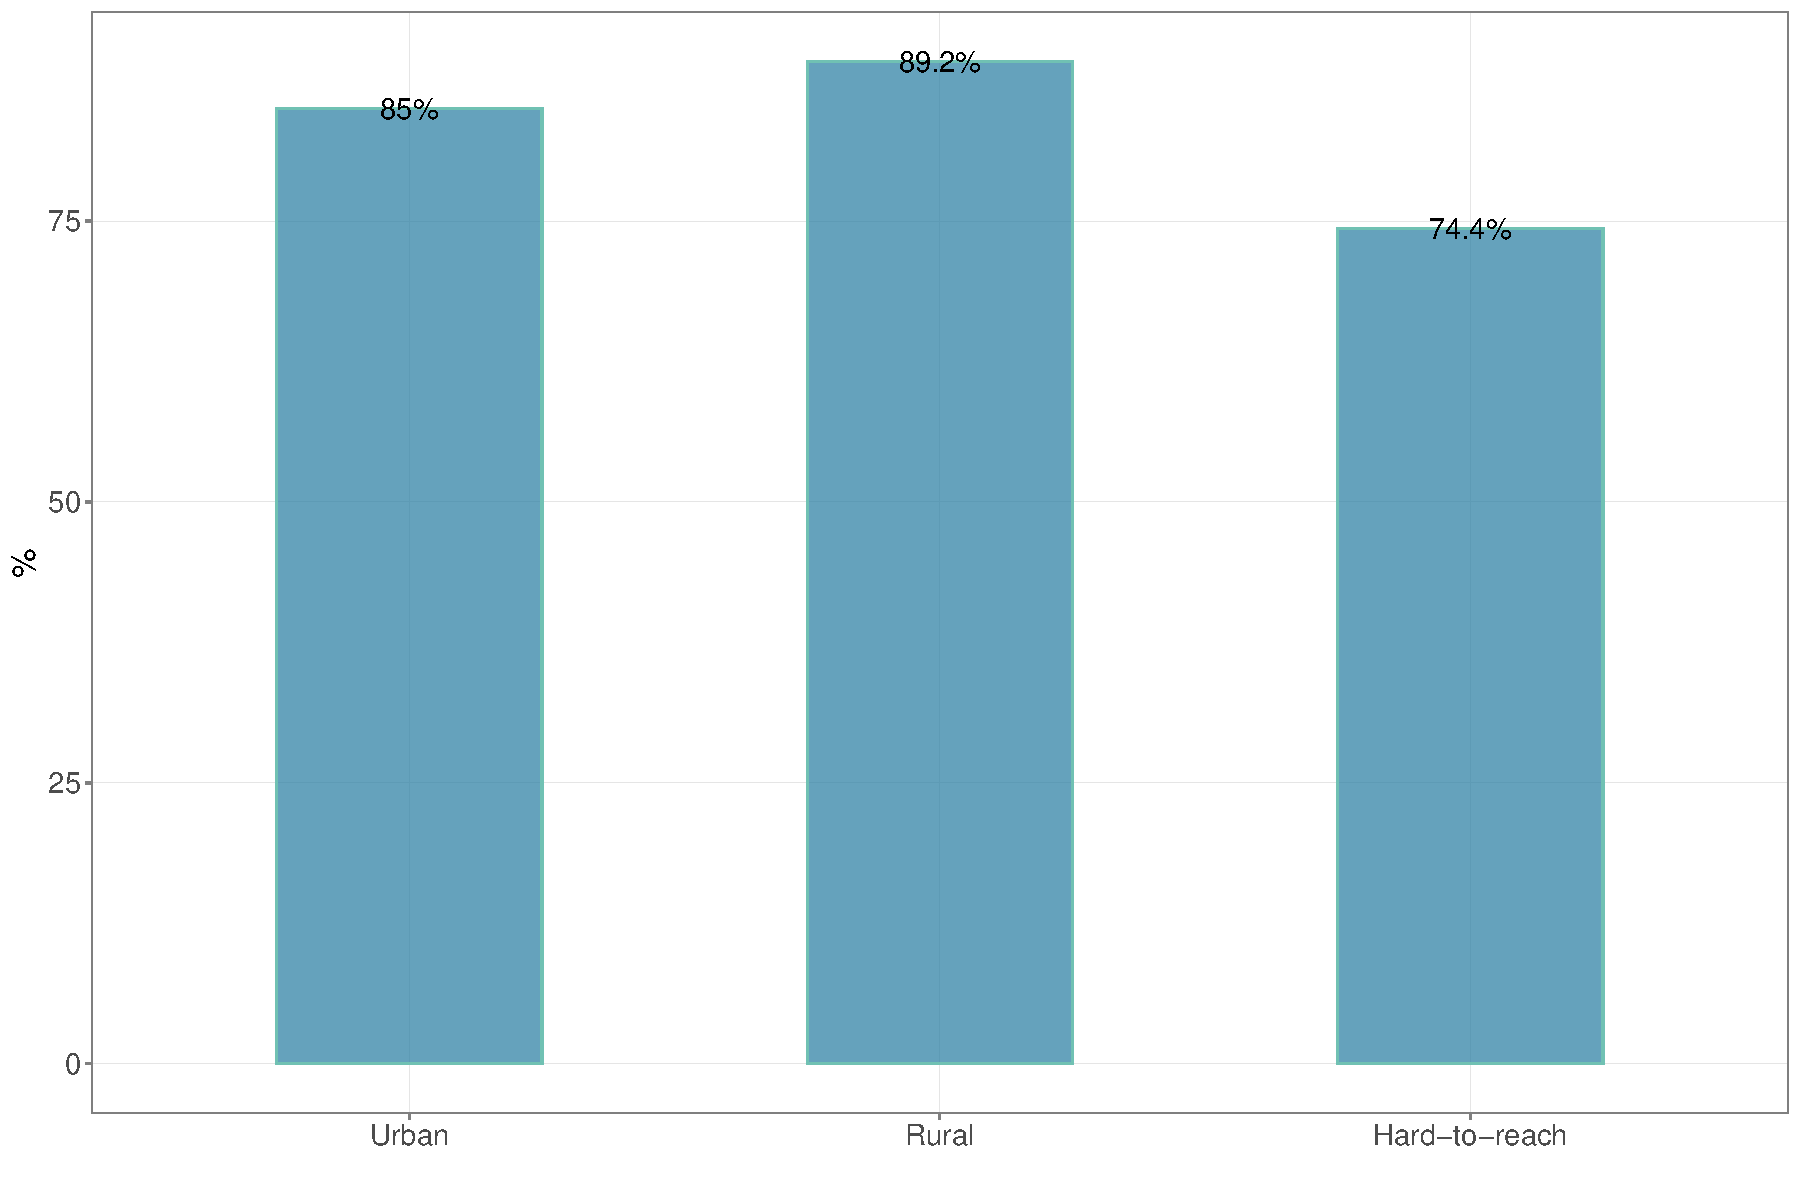
\includegraphics{kayinReport_files/figure-latex/ari1plot-1} 

}

\caption{Treatment-seeking for acute respiratory infection by location type}\label{fig:ari1plot}
\end{figure}

\begin{figure}[H]

{\centering 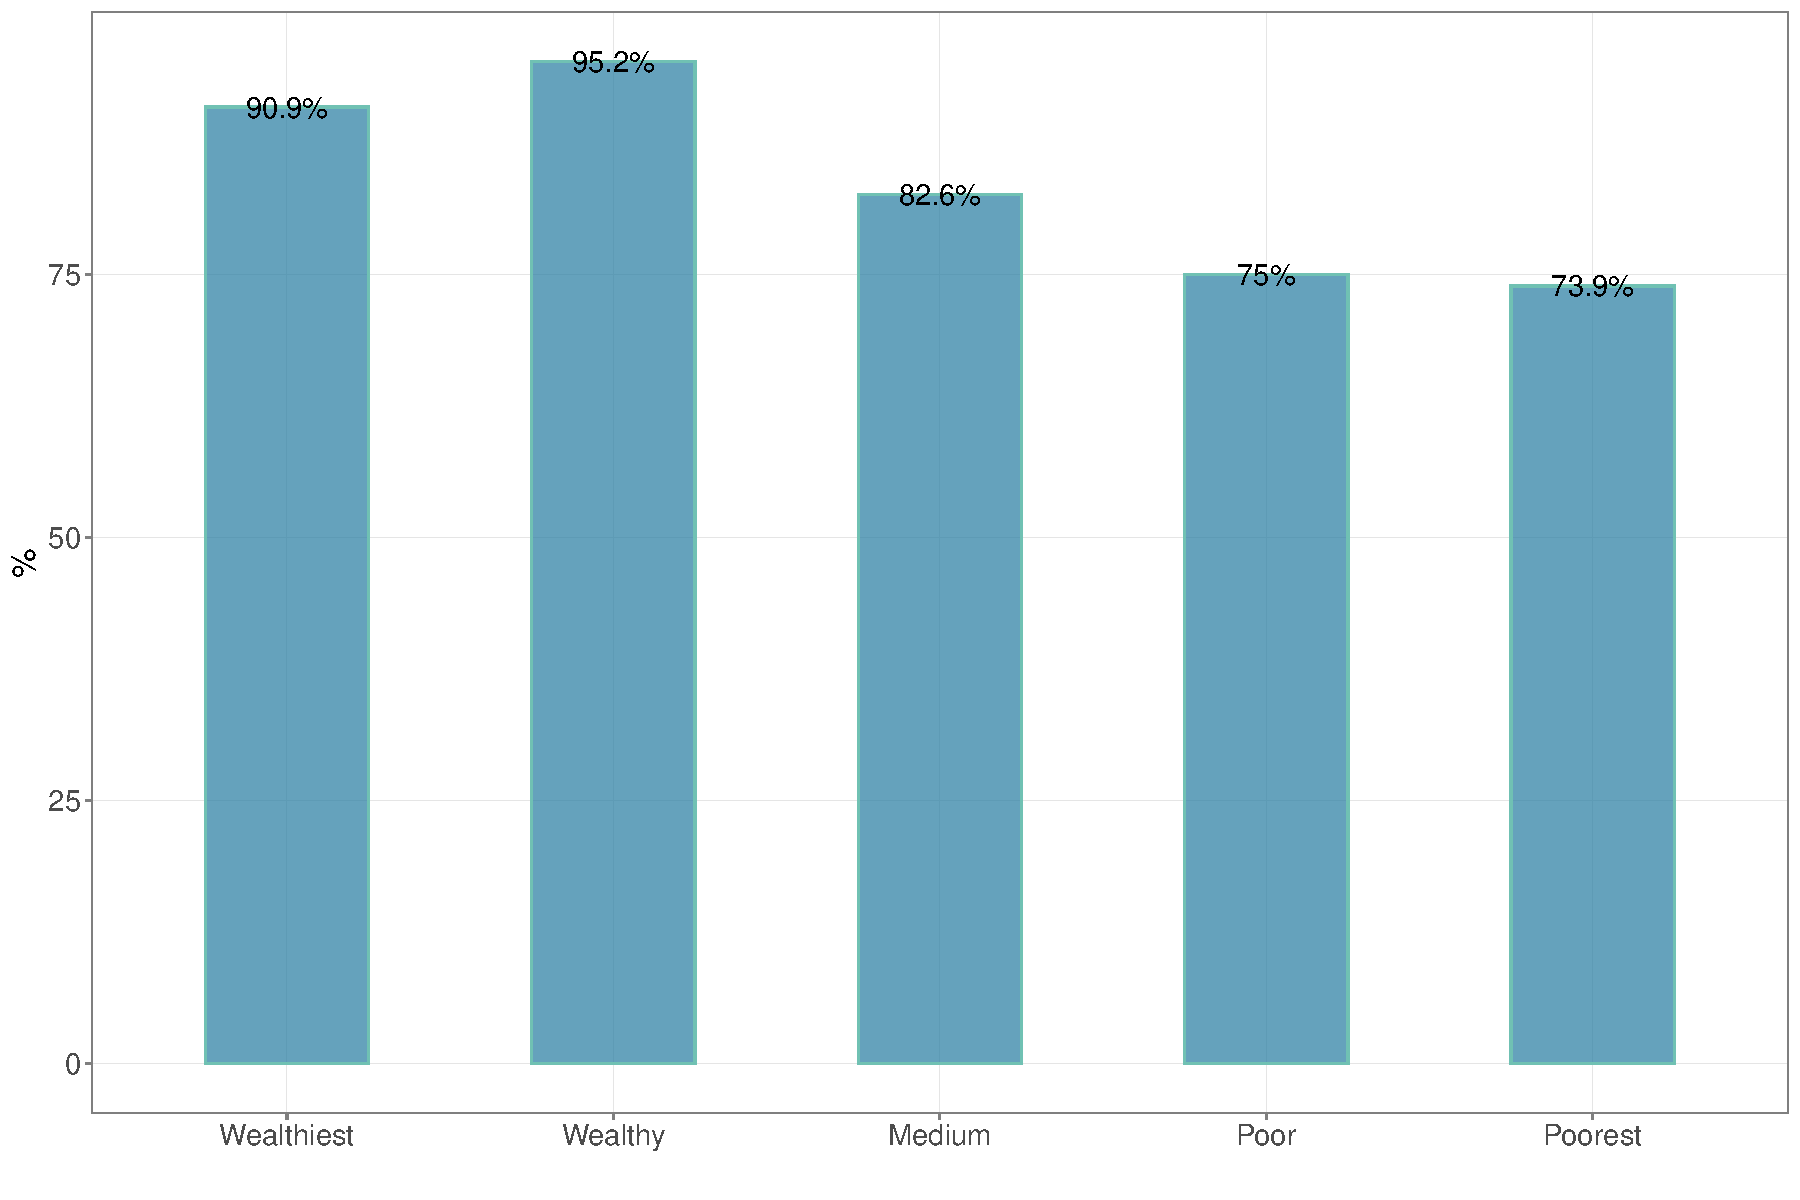
\includegraphics{kayinReport_files/figure-latex/ari2plot-1} 

}

\caption{Treatment-seeking for acute respiratory infection by wealth quintiles}\label{fig:ari2plot}
\end{figure}

\begin{figure}[H]

{\centering 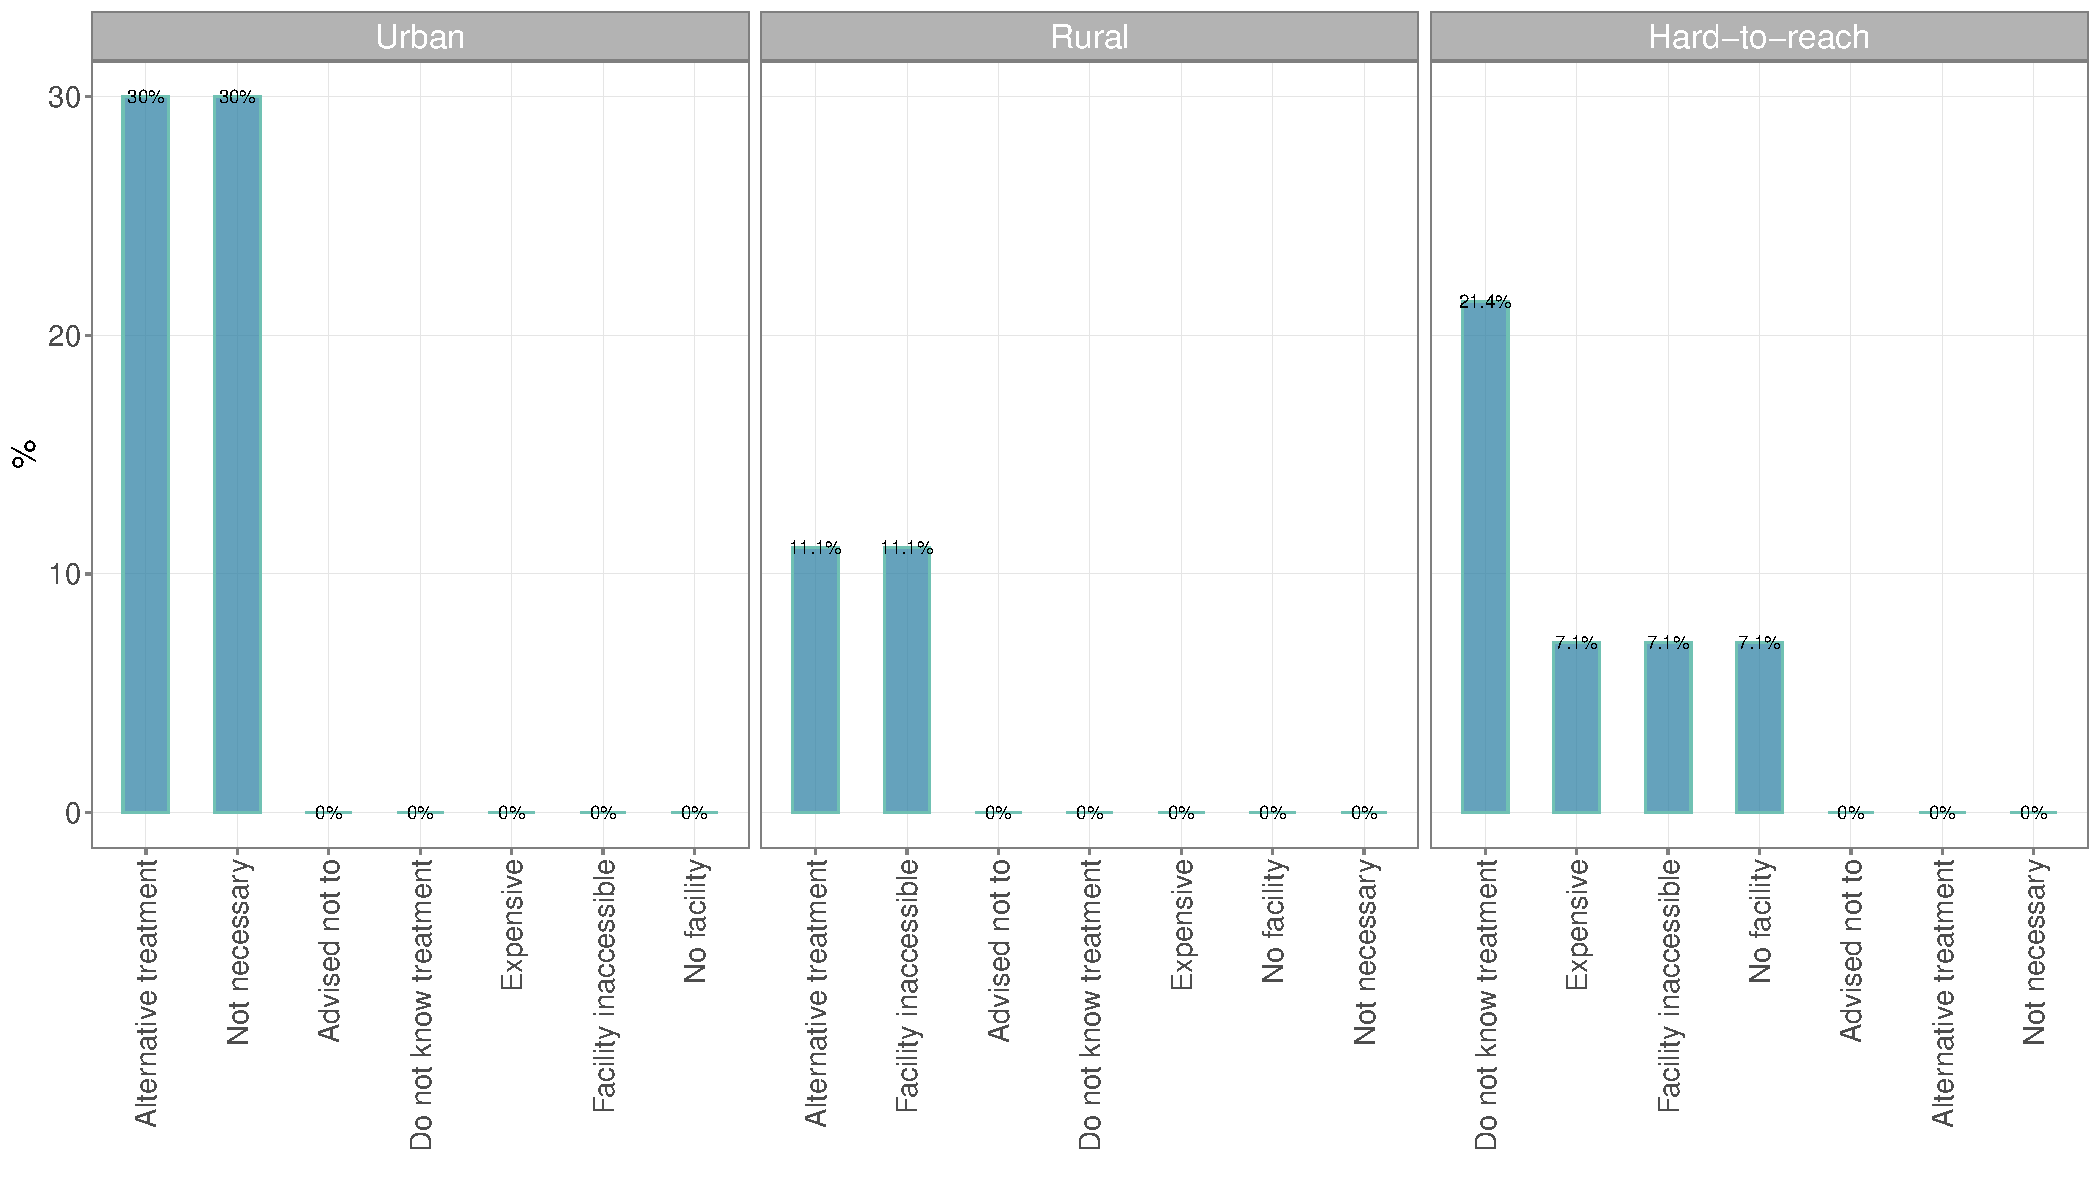
\includegraphics{kayinReport_files/figure-latex/ari3plot-1} 

}

\caption{Reasons for not seeking treatment by location type}\label{fig:ari3plot}
\end{figure}

\begin{figure}[H]

{\centering 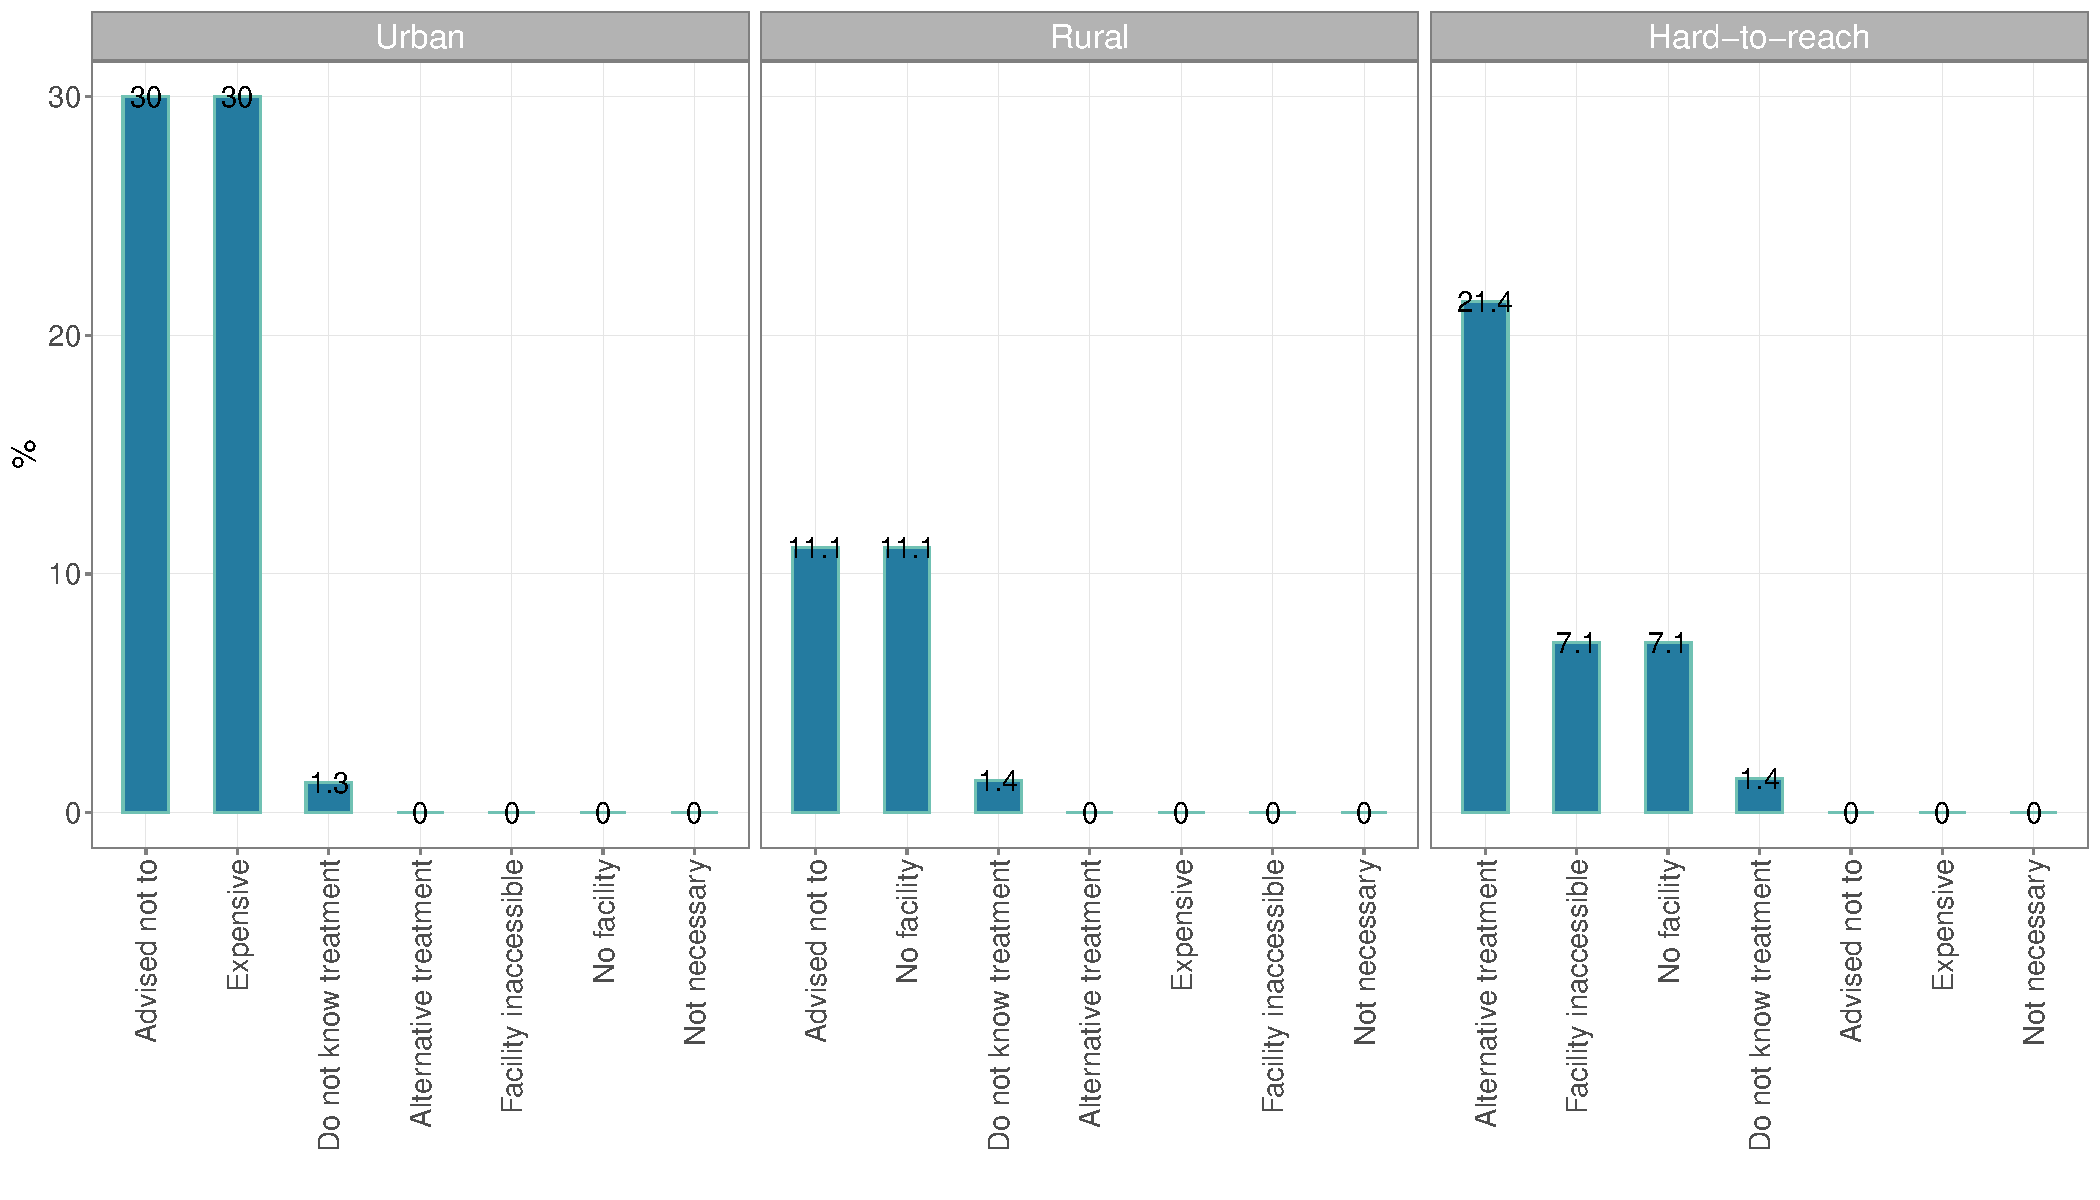
\includegraphics{kayinReport_files/figure-latex/ari4plot-1} 

}

\caption{Reasons for not seeking treatment by wealth quintile}\label{fig:ari4plot}
\end{figure}

\begin{landscape}\begin{table}[H]

\caption{\label{tab:ari2table}Where/who treatment is sought from}
\centering
\fontsize{9}{11}\selectfont
\begin{tabular}[t]{>{\bfseries}l>{\bfseries}l>{\ttfamily}r>{\ttfamily}r>{\ttfamily}r>{\ttfamily}r>{\ttfamily}r>{\ttfamily}r>{\ttfamily}r>{\ttfamily}r>{\ttfamily}r>{\ttfamily}r>{\ttfamily}r>{\ttfamily}r>{\ttfamily}r}
\toprule
\multicolumn{2}{c}{\textbf{ }} & \multicolumn{13}{c}{\textbf{Where/who treatment is sought from}} \\
\cmidrule(l{3pt}r{3pt}){3-15}
 &  & \makecell[c]{Township\\hospital\\(\%)} & \makecell[c]{Station\\hospital\\(\%)} & \makecell[c]{RHC/\\health\\assistant\\(\%)} & \makecell[c]{SRHC/\\midwife\\(\%)} & \makecell[c]{Private\\clinic/\\doctor\\(\%)} & \makecell[c]{Community\\health\\worker\\(\%)} & \makecell[c]{Traditional\\healer\\(\%)} & \makecell[c]{Untrained\\health\\worker\\(\%)} & \makecell[c]{Drug\\from\\shop\\(\%)} & \makecell[c]{EHO\\clinic/\\volunteer\\(\%)} & \makecell[c]{Family\\member\\(\%)} & \makecell[c]{NGOs/\\clinic\\(\%)} & \makecell[c]{Auxilliary\\midwife\\(\%)}\\
\midrule
\addlinespace[0.3em]
\multicolumn{15}{l}{\textbf{Kayin}}\\
\addlinespace[0.3em]
\multicolumn{15}{l}{\textit{\textbf{Geographic}}}\\
\hspace{1em}\hspace{1em} & Rural & 1.7 & 8.3 & 18.3 & 18.3 & 21.7 & 5.0 & 0.0 & 0 & 18.3 & 0.0 & 0.0 & 0 & 5.0\\
\cmidrule{2-15}
\hspace{1em}\hspace{1em} & Urban & 3.8 & 0.0 & 1.9 & 0.0 & 73.1 & 0.0 & 0.0 & 0 & 1.9 & 1.9 & 0.0 & 0 & 0.0\\
\cmidrule{2-15}
\hspace{1em}\hspace{1em} & Hard-to-reach & 1.3 & 8.0 & 0.0 & 2.7 & 10.7 & 10.7 & 2.7 & 0 & 25.3 & 26.7 & 2.7 & 0 & 1.3\\
\cmidrule{2-15}
\addlinespace[0.3em]
\multicolumn{15}{l}{\textit{\textbf{Wealth}}}\\
\hspace{1em}\hspace{1em} & Wealthiest & 3.6 & 0.0 & 3.6 & 0.0 & 57.1 & 0.0 & 0.0 & 0 & 3.6 & 3.6 & 0.0 & 0 & 0.0\\
\cmidrule{2-15}
\hspace{1em}\hspace{1em} & Wealthy & 2.4 & 9.5 & 9.5 & 2.4 & 42.9 & 2.4 & 2.4 & 0 & 7.1 & 2.4 & 4.8 & 0 & 2.4\\
\cmidrule{2-15}
\hspace{1em}\hspace{1em} & Medium & 0.0 & 7.3 & 7.3 & 9.8 & 31.7 & 9.8 & 0.0 & 0 & 17.1 & 9.8 & 0.0 & 0 & 0.0\\
\cmidrule{2-15}
\hspace{1em}\hspace{1em} & Poor & 2.4 & 4.9 & 7.3 & 9.8 & 9.8 & 9.8 & 0.0 & 0 & 34.1 & 12.2 & 0.0 & 0 & 7.3\\
\cmidrule{2-15}
\hspace{1em}\hspace{1em} & Poorest & 3.0 & 6.1 & 3.0 & 12.1 & 18.2 & 6.1 & 3.0 & 0 & 18.2 & 30.3 & 0.0 & 0 & 0.0\\
\bottomrule
\end{tabular}
\end{table}
\end{landscape}

\begin{figure}[H]

{\centering 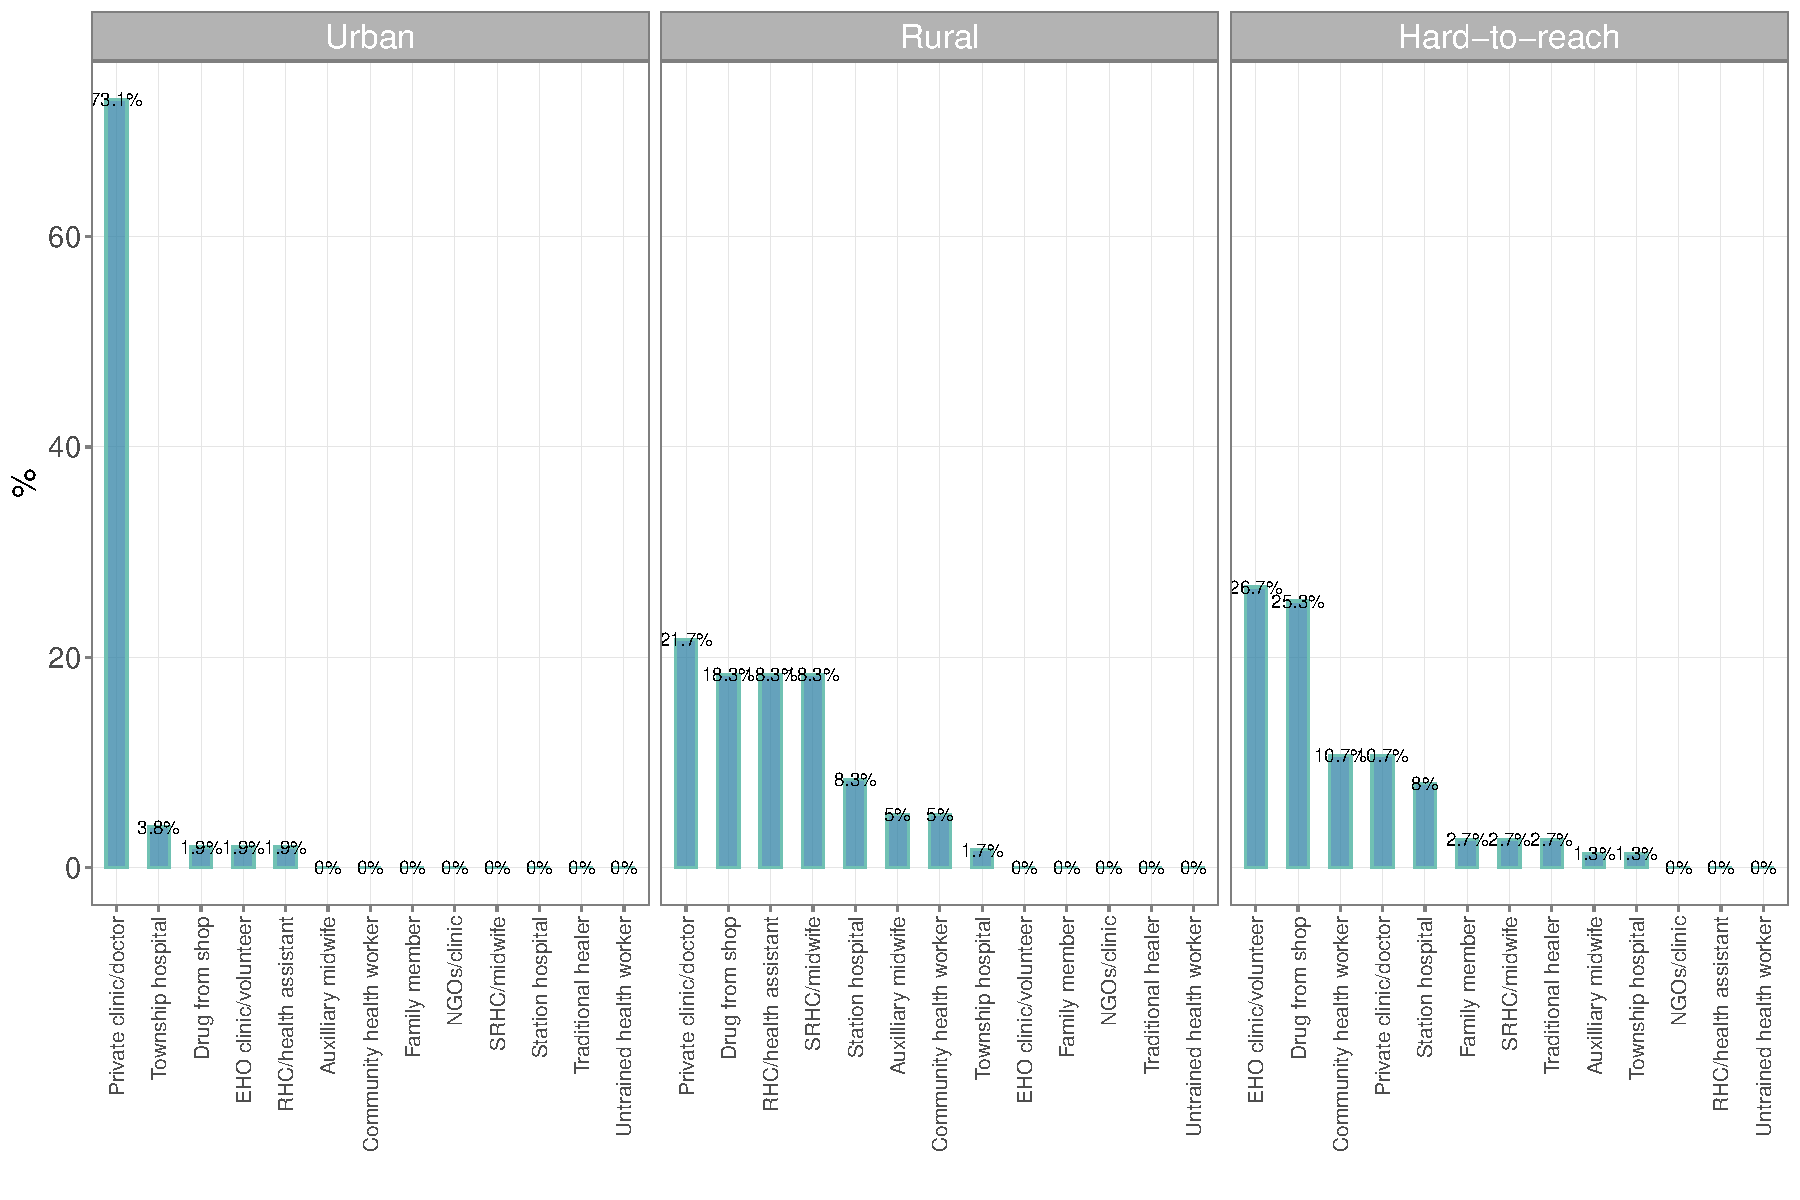
\includegraphics{kayinReport_files/figure-latex/ari5plot-1} 

}

\caption{Where/who treatment is sought from by location type}\label{fig:ari5plot}
\end{figure}

\begin{figure}[H]

{\centering 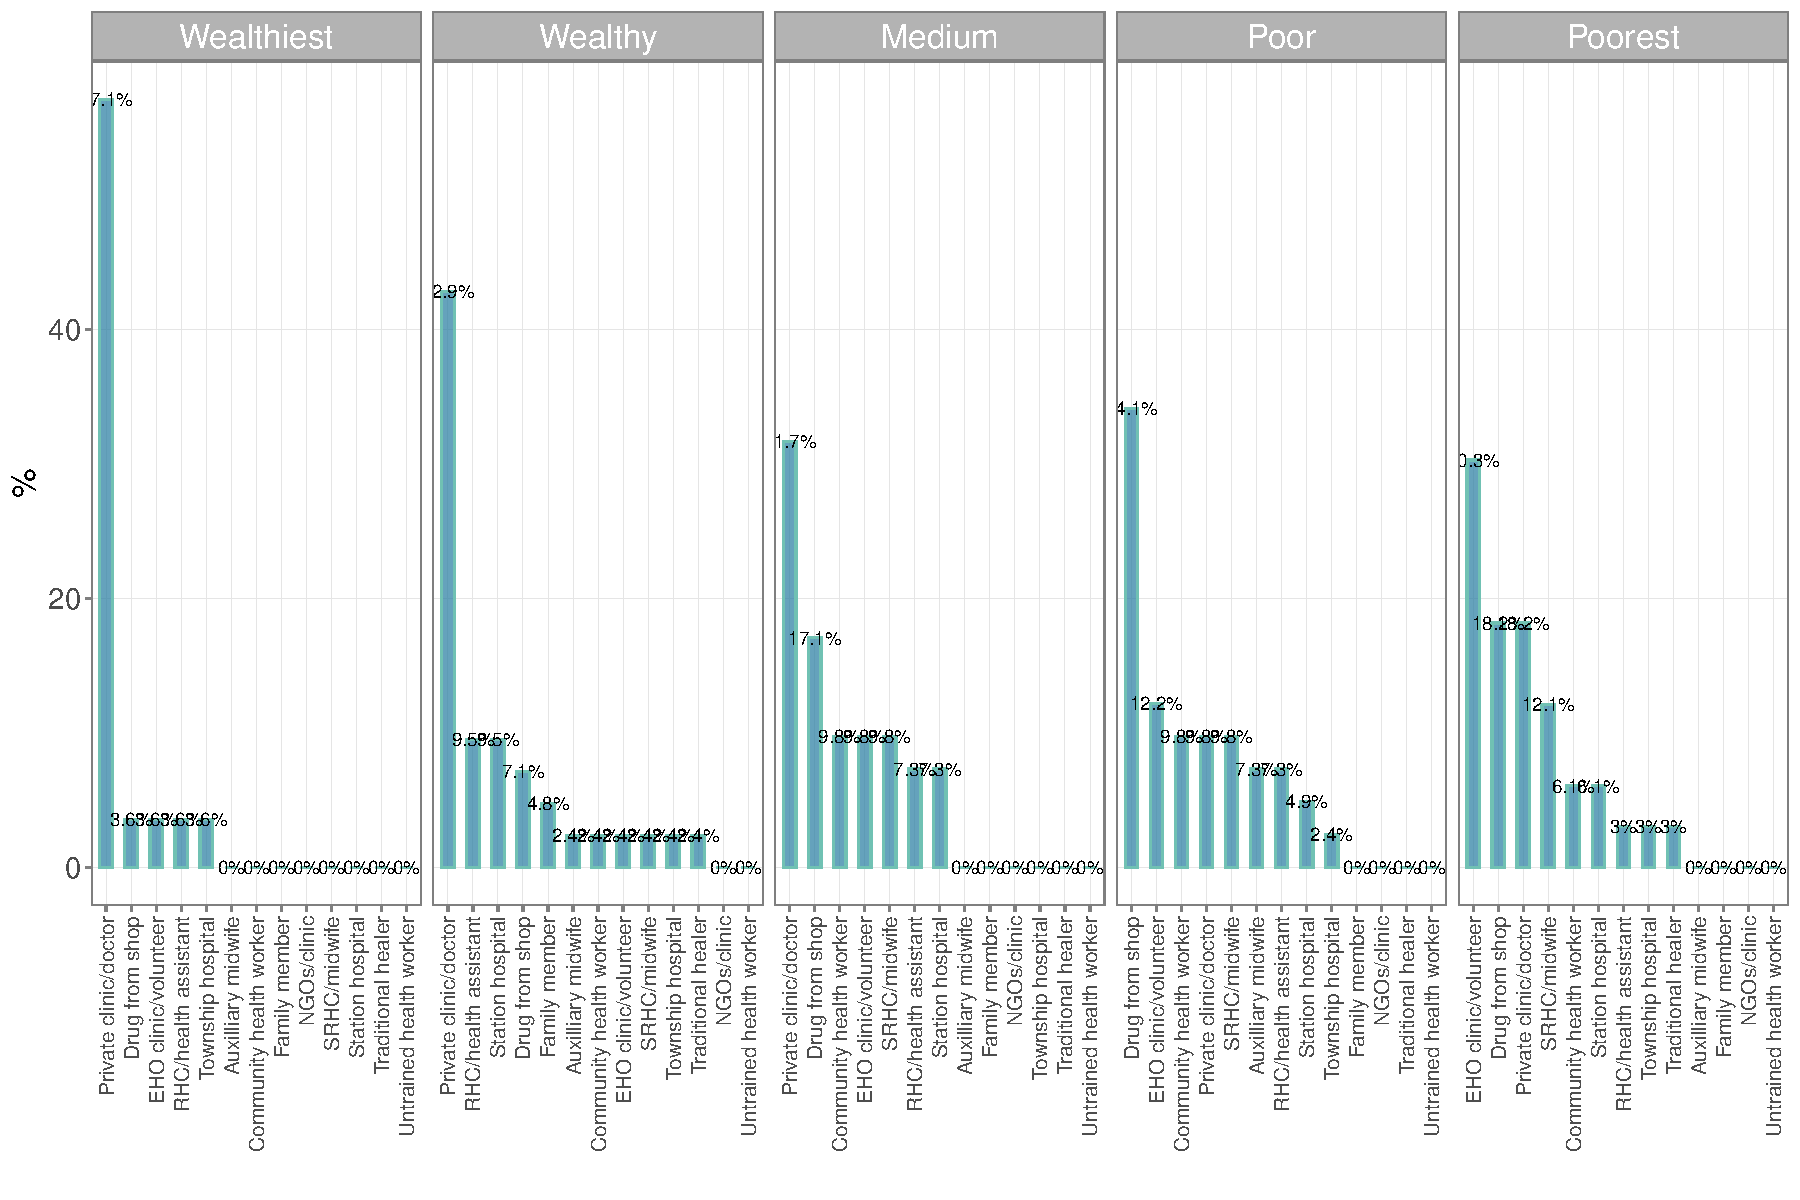
\includegraphics{kayinReport_files/figure-latex/ari6plot-1} 

}

\caption{Where/who treatment is sought from by wealth quintiles}\label{fig:ari6plot}
\end{figure}

\begin{landscape}\begin{table}[H]

\caption{\label{tab:ari3table}Payment for treatment}
\centering
\fontsize{10}{12}\selectfont
\begin{tabular}[t]{>{\bfseries}l>{\bfseries}l>{\ttfamily}r>{\ttfamily}r>{\ttfamily}r>{\ttfamily}r>{\ttfamily}r>{\ttfamily}r>{\ttfamily}r>{\ttfamily}r}
\toprule
\multicolumn{3}{c}{\textbf{ }} & \multicolumn{6}{c}{\textbf{Payment for}} & \multicolumn{1}{c}{\textbf{ }} \\
\cmidrule(l{3pt}r{3pt}){4-9}
 &  & \makecell[c]{Payment\\for\\service\\(MMK)} & \makecell[c]{Transportation\\(\%)} & \makecell[c]{Registration\\(\%)} & \makecell[c]{Medicine\\(\%)} & \makecell[c]{Laboratory\\fees\\(\%)} & \makecell[c]{Provider\\fees\\(\%)} & \makecell[c]{Gifts\\(\%)} & \makecell[c]{Took\\loan\\(\%)}\\
\midrule
\addlinespace[0.3em]
\multicolumn{10}{l}{\textbf{Kayin}}\\
\addlinespace[0.3em]
\multicolumn{10}{l}{\textit{\textbf{Geographic}}}\\
\hspace{1em}\hspace{1em} & Rural & 7076.7 & 0.0 & 0.0 & 100.0 & 0 & 0 & 0 & 3.8\\
\cmidrule{2-10}
\hspace{1em}\hspace{1em} & Urban & 12245.1 & 0.0 & 0.0 & 100.0 & 0 & 0 & 0 & 6.0\\
\cmidrule{2-10}
\hspace{1em}\hspace{1em} & Hard-to-reach & 5360.0 & 2.6 & 2.6 & 92.3 & 0 & 0 & 0 & 11.1\\
\cmidrule{2-10}
\addlinespace[0.3em]
\multicolumn{10}{l}{\textit{\textbf{Wealth}}}\\
\hspace{1em}\hspace{1em} & Wealthiest & 13648.1 & 0.0 & 0.0 & 100.0 & 0 & 0 & 0 & 3.8\\
\cmidrule{2-10}
\hspace{1em}\hspace{1em} & Wealthy & 9154.8 & 0.0 & 0.0 & 100.0 & 0 & 0 & 0 & 2.5\\
\cmidrule{2-10}
\hspace{1em}\hspace{1em} & Medium & 8739.0 & 0.0 & 0.0 & 95.7 & 0 & 0 & 0 & 5.9\\
\cmidrule{2-10}
\hspace{1em}\hspace{1em} & Poor & 3982.9 & 0.0 & 0.0 & 100.0 & 0 & 0 & 0 & 14.7\\
\cmidrule{2-10}
\hspace{1em}\hspace{1em} & Poorest & 4590.9 & 6.7 & 6.7 & 86.7 & 0 & 0 & 0 & 9.5\\
\bottomrule
\end{tabular}
\end{table}
\end{landscape}

\begin{figure}[H]

{\centering 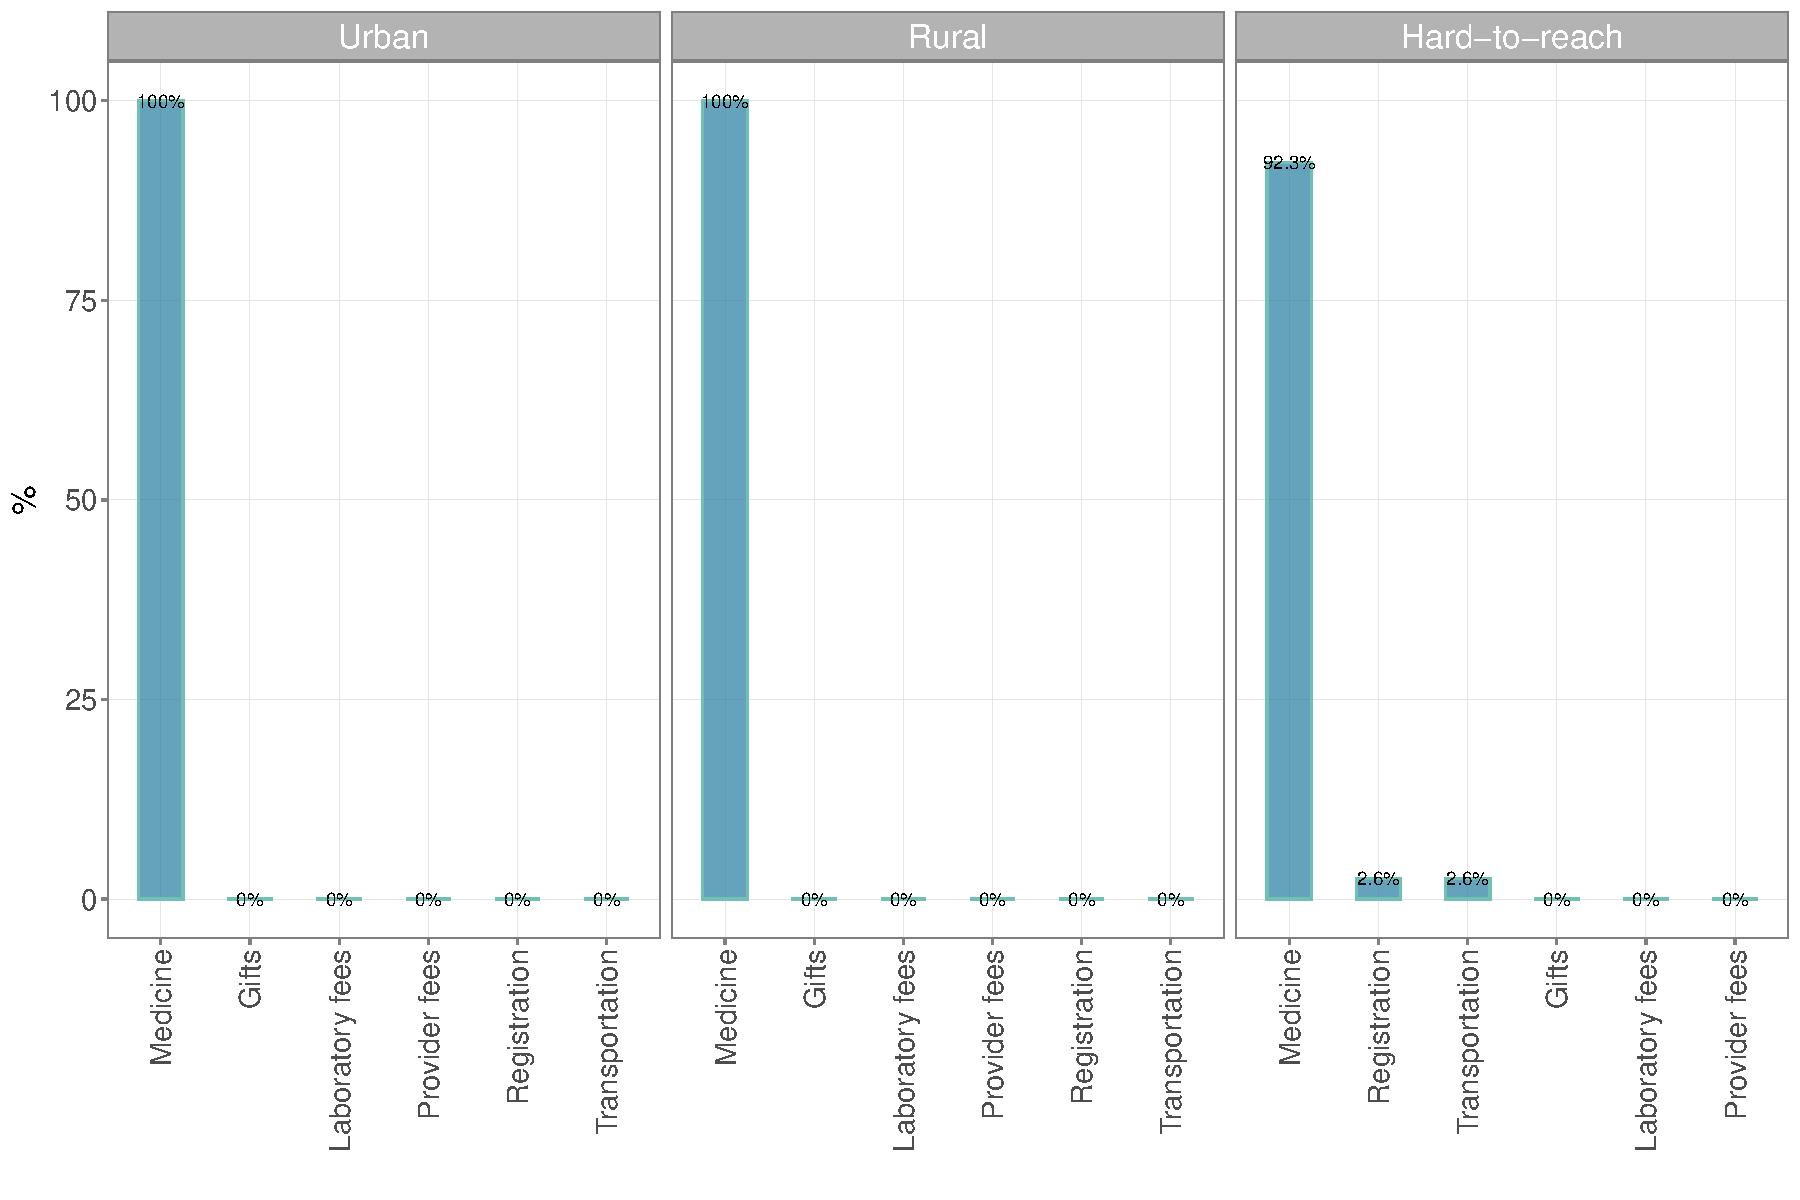
\includegraphics{kayinReport_files/figure-latex/ari7plot-1} 

}

\caption{Costs incurred for treatment by location type}\label{fig:ari7plot}
\end{figure}

\begin{figure}[H]

{\centering 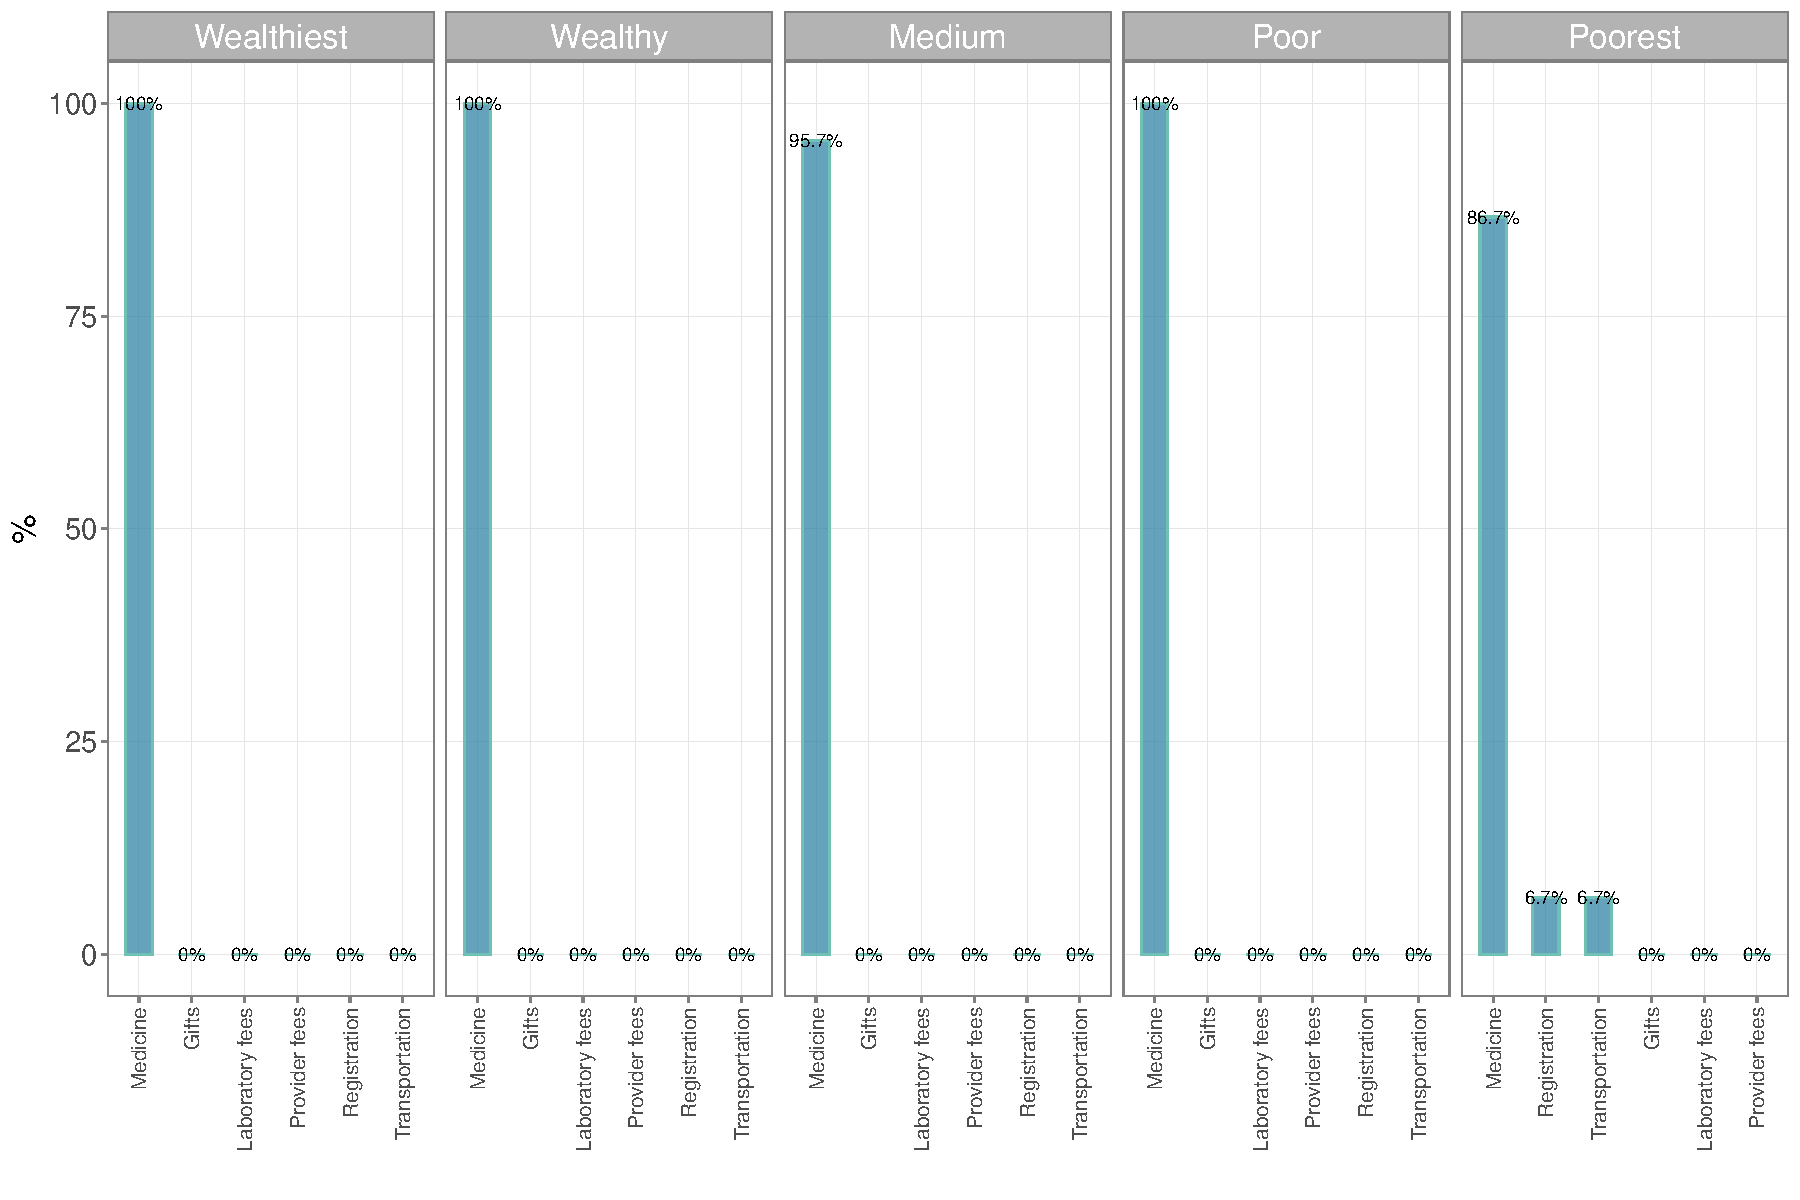
\includegraphics{kayinReport_files/figure-latex/ari8plot-1} 

}

\caption{Costs incurred for treatment by wealth quintiles}\label{fig:ari8plot}
\end{figure}

\hypertarget{fever}{%
\subparagraph{Fever}\label{fever}}

Treatment-seeking for fever in Kayin state can be characterised by households in urban and rural areas seeking treatment the most (91\% and 94\% respectively) whilst those in hard-to-reach areas seeking treatment slightly lesser (see Figure \ref{fig:fever1plot}). Most of households across wealth classes sought treatment for fever with the poorest households seeking care the least at 80\% (see Figure \ref{fig:fever2plot}).

When asked why treatment was not sought for fever, those from the urban areas thought that treatment was not necessary or sought alternative treatment. Households in rural areas also sought alternative treatment. Hard-to-reach households, on the other hand, had issues accesing facilities and are not aware of treatment for fever (see Figure \ref{fig:fever3plot}). Most households across wealth classes sought alternative treatment except for poorest households who thought treatment was not necessary and who found health facilities inaccessible or expensive (see Figure \ref{fig:fever4plot}). Time to treatment is generally the same between households in different location types and across wealth classes at about 1 day to treatment (see Table \ref{tab:fever1table}).

Those from urban and rural areas tended to see a private doctor, those from rural areas would often visit their SRHC and those from hard-to-reach areas predominantly went to their EHO clinic (see Figure \ref{fig:fever5plot}). Wealthier households often sought treatment from private doctor and the poorest households visit the SRHC or self-medicate (see Figure \ref{fig:fever6plot}.

Costs incurred for treatment were majority for medications (see Table \ref{tab:fever3table}, Figure \ref{fig:fever7plot} and Figure \ref{fig:fever8plot}).

\begin{landscape}\begin{table}[H]

\caption{\label{tab:fever1table}Treatment-seeking for fever}
\centering
\fontsize{10}{12}\selectfont
\begin{tabular}[t]{>{\bfseries}l>{\bfseries}l>{\ttfamily}r>{\ttfamily}r>{\ttfamily}r>{\ttfamily}r>{\ttfamily}r>{\ttfamily}r>{\ttfamily}r>{\ttfamily}r>{\ttfamily}r}
\toprule
\multicolumn{4}{c}{\textbf{ }} & \multicolumn{7}{c}{\textbf{Reasons for not seeking treatment}} \\
\cmidrule(l{3pt}r{3pt}){5-11}
 &  & \makecell[c]{Sought\\treatment\\(\%)} & \makecell[c]{Time to\\treatment\\(days)} & \makecell[c]{No\\facility\\(\%)} & \makecell[c]{Facility\\inaccessible\\(\%)} & \makecell[c]{Expensive\\(\%)} & \makecell[c]{Not\\necessary\\(\%)} & \makecell[c]{Advised\\not to\\(\%)} & \makecell[c]{Alternative\\treatment\\(\%)} & \makecell[c]{Do not know\\treamtent\\(\%)}\\
\midrule
\addlinespace[0.3em]
\multicolumn{11}{l}{\textbf{Kayin}}\\
\addlinespace[0.3em]
\multicolumn{11}{l}{\textit{\textbf{Geographic}}}\\
\hspace{1em}\hspace{1em} & Rural & 94.0 & 1.1 & 0.0 & 0.0 & 8.3 & 8.3 & 0 & 25.0 & 0.0\\
\cmidrule{2-11}
\hspace{1em}\hspace{1em} & Urban & 91.3 & 1.2 & 0.0 & 0.0 & 0.0 & 18.8 & 0 & 18.8 & 0.0\\
\cmidrule{2-11}
\hspace{1em}\hspace{1em} & Hard-to-reach & 79.0 & 1.4 & 5.0 & 10.0 & 5.0 & 5.0 & 0 & 0.0 & 5.0\\
\cmidrule{2-11}
\addlinespace[0.3em]
\multicolumn{11}{l}{\textit{\textbf{Wealth}}}\\
\hspace{1em}\hspace{1em} & Wealthiest & 91.0 & 1.1 & 0.0 & 0.0 & 0.0 & 0.0 & 0 & 22.2 & 0.0\\
\cmidrule{2-11}
\hspace{1em}\hspace{1em} & Wealthy & 90.3 & 1.3 & 0.0 & 0.0 & 11.1 & 11.1 & 0 & 11.1 & 0.0\\
\cmidrule{2-11}
\hspace{1em}\hspace{1em} & Medium & 92.9 & 1.1 & 0.0 & 0.0 & 0.0 & 14.3 & 0 & 14.3 & 0.0\\
\cmidrule{2-11}
\hspace{1em}\hspace{1em} & Poor & 92.9 & 1.2 & 0.0 & 0.0 & 0.0 & 0.0 & 0 & 28.6 & 14.3\\
\cmidrule{2-11}
\hspace{1em}\hspace{1em} & Poorest & 79.2 & 1.5 & 6.2 & 12.5 & 6.2 & 18.8 & 0 & 0.0 & 0.0\\
\bottomrule
\end{tabular}
\end{table}
\end{landscape}

\begin{figure}[H]

{\centering \includegraphics{kayinReport_files/figure-latex/fever1plot-1} 

}

\caption{Treatment-seeking for fever by location type}\label{fig:fever1plot}
\end{figure}

\begin{figure}[H]

{\centering \includegraphics{kayinReport_files/figure-latex/fever2plot-1} 

}

\caption{Treatment-seeking for fever by wealth quintiles}\label{fig:fever2plot}
\end{figure}

\begin{figure}[H]

{\centering \includegraphics{kayinReport_files/figure-latex/fever3plot-1} 

}

\caption{Reasons for not seeking treatment by location type}\label{fig:fever3plot}
\end{figure}

\begin{figure}[H]

{\centering \includegraphics{kayinReport_files/figure-latex/fever4plot-1} 

}

\caption{Reasons for not seeking treatment by wealth quintiles}\label{fig:fever4plot}
\end{figure}

\begin{landscape}\begin{table}[H]

\caption{\label{tab:fever2table}Where/who treatment is sought from}
\centering
\fontsize{9}{11}\selectfont
\begin{tabular}[t]{>{\bfseries}l>{\bfseries}l>{\ttfamily}r>{\ttfamily}r>{\ttfamily}r>{\ttfamily}r>{\ttfamily}r>{\ttfamily}r>{\ttfamily}r>{\ttfamily}r>{\ttfamily}r>{\ttfamily}r>{\ttfamily}r>{\ttfamily}r>{\ttfamily}r}
\toprule
\multicolumn{2}{c}{\textbf{ }} & \multicolumn{13}{c}{\textbf{Where/who treatment is sought from}} \\
\cmidrule(l{3pt}r{3pt}){3-15}
 &  & \makecell[c]{Township\\hospital\\(\%)} & \makecell[c]{Station\\hospital\\(\%)} & \makecell[c]{RHC/\\health\\assistant\\(\%)} & \makecell[c]{SRHC/\\midwife\\(\%)} & \makecell[c]{Private\\clinic/\\doctor\\(\%)} & \makecell[c]{Community\\health\\worker\\(\%)} & \makecell[c]{Traditional\\healer\\(\%)} & \makecell[c]{Untrained\\health\\worker\\(\%)} & \makecell[c]{Drug\\from\\shop\\(\%)} & \makecell[c]{EHO\\clinic/\\volunteer\\(\%)} & \makecell[c]{Family\\member\\(\%)} & \makecell[c]{NGOs/\\clinic\\(\%)} & \makecell[c]{Auxilliary\\midwife\\(\%)}\\
\midrule
\addlinespace[0.3em]
\multicolumn{15}{l}{\textbf{Kayin}}\\
\addlinespace[0.3em]
\multicolumn{15}{l}{\textit{\textbf{Geographic}}}\\
\hspace{1em}\hspace{1em} & Rural & 3.5 & 5.6 & 17.5 & 25.2 & 17.5 & 2.1 & 0.7 & 2.8 & 12.6 & 0.0 & 2.8 & 0 & 3.5\\
\cmidrule{2-15}
\hspace{1em}\hspace{1em} & Urban & 3.6 & 0.7 & 1.5 & 0.0 & 82.5 & 0.7 & 0.0 & 0.0 & 4.4 & 0.0 & 0.0 & 0 & 0.0\\
\cmidrule{2-15}
\hspace{1em}\hspace{1em} & Hard-to-reach & 2.0 & 7.0 & 1.0 & 7.0 & 11.0 & 9.0 & 1.0 & 1.0 & 22.0 & 29.0 & 2.0 & 0 & 3.0\\
\cmidrule{2-15}
\addlinespace[0.3em]
\multicolumn{15}{l}{\textit{\textbf{Wealth}}}\\
\hspace{1em}\hspace{1em} & Wealthiest & 2.8 & 2.8 & 2.8 & 0.0 & 77.5 & 0.0 & 0.0 & 0.0 & 4.2 & 0.0 & 0.0 & 0 & 0.0\\
\cmidrule{2-15}
\hspace{1em}\hspace{1em} & Wealthy & 3.4 & 5.7 & 6.9 & 8.0 & 54.0 & 1.1 & 0.0 & 1.1 & 5.7 & 3.4 & 3.4 & 0 & 0.0\\
\cmidrule{2-15}
\hspace{1em}\hspace{1em} & Medium & 2.2 & 5.5 & 7.7 & 17.6 & 22.0 & 7.7 & 0.0 & 4.4 & 11.0 & 11.0 & 2.2 & 0 & 2.2\\
\cmidrule{2-15}
\hspace{1em}\hspace{1em} & Poor & 4.5 & 6.1 & 16.7 & 18.2 & 16.7 & 4.5 & 1.5 & 0.0 & 15.2 & 9.1 & 0.0 & 0 & 3.0\\
\cmidrule{2-15}
\hspace{1em}\hspace{1em} & Poorest & 0.0 & 0.0 & 3.5 & 14.0 & 19.3 & 3.5 & 1.8 & 0.0 & 31.6 & 17.5 & 0.0 & 0 & 7.0\\
\bottomrule
\end{tabular}
\end{table}
\end{landscape}

\begin{figure}[H]

{\centering \includegraphics{kayinReport_files/figure-latex/fever5plot-1} 

}

\caption{Where/who treatment is sought from by location type}\label{fig:fever5plot}
\end{figure}

\begin{figure}[H]

{\centering \includegraphics{kayinReport_files/figure-latex/fever6plot-1} 

}

\caption{Where/who treatment is sought from by wealth quintiles}\label{fig:fever6plot}
\end{figure}

\begin{landscape}\begin{table}[H]

\caption{\label{tab:fever3table}Payment for treatment}
\centering
\fontsize{10}{12}\selectfont
\begin{tabular}[t]{>{\bfseries}l>{\bfseries}l>{\ttfamily}r>{\ttfamily}r>{\ttfamily}r>{\ttfamily}r>{\ttfamily}r>{\ttfamily}r>{\ttfamily}r>{\ttfamily}r}
\toprule
\multicolumn{3}{c}{\textbf{ }} & \multicolumn{6}{c}{\textbf{Payment for}} & \multicolumn{1}{c}{\textbf{ }} \\
\cmidrule(l{3pt}r{3pt}){4-9}
 &  & \makecell[c]{Payment\\for\\service\\(MMK)} & \makecell[c]{Transportation\\(\%)} & \makecell[c]{Registration\\(\%)} & \makecell[c]{Medicine\\(\%)} & \makecell[c]{Laboratory\\fees\\(\%)} & \makecell[c]{Provider\\fees\\(\%)} & \makecell[c]{Gifts\\(\%)} & \makecell[c]{Took\\loan\\(\%)}\\
\midrule
\addlinespace[0.3em]
\multicolumn{10}{l}{\textbf{Kayin}}\\
\addlinespace[0.3em]
\multicolumn{10}{l}{\textit{\textbf{Geographic}}}\\
\hspace{1em}\hspace{1em} & Rural & 13290.0 & 1.2 & 0 & 97.5 & 0 & 0 & 0 & 9.9\\
\cmidrule{2-10}
\hspace{1em}\hspace{1em} & Urban & 13923.4 & 0.0 & 0 & 100.0 & 0 & 0 & 0 & 12.8\\
\cmidrule{2-10}
\hspace{1em}\hspace{1em} & Hard-to-reach & 8271.0 & 5.5 & 0 & 94.5 & 0 & 0 & 0 & 8.5\\
\cmidrule{2-10}
\addlinespace[0.3em]
\multicolumn{10}{l}{\textit{\textbf{Wealth}}}\\
\hspace{1em}\hspace{1em} & Wealthiest & 17457.7 & 0.0 & 0 & 100.0 & 0 & 0 & 0 & 5.7\\
\cmidrule{2-10}
\hspace{1em}\hspace{1em} & Wealthy & 11106.9 & 2.6 & 0 & 94.7 & 0 & 0 & 0 & 6.2\\
\cmidrule{2-10}
\hspace{1em}\hspace{1em} & Medium & 7017.8 & 0.0 & 0 & 100.0 & 0 & 0 & 0 & 10.5\\
\cmidrule{2-10}
\hspace{1em}\hspace{1em} & Poor & 19218.8 & 4.9 & 0 & 95.1 & 0 & 0 & 0 & 19.0\\
\cmidrule{2-10}
\hspace{1em}\hspace{1em} & Poorest & 5154.4 & 3.1 & 0 & 96.9 & 0 & 0 & 0 & 13.6\\
\bottomrule
\end{tabular}
\end{table}
\end{landscape}

\begin{figure}[H]

{\centering \includegraphics{kayinReport_files/figure-latex/fever7plot-1} 

}

\caption{Costs incurred for treatment by location type}\label{fig:fever7plot}
\end{figure}

\begin{figure}[H]

{\centering \includegraphics{kayinReport_files/figure-latex/fever8plot-1} 

}

\caption{Costs incurred for treatment by wealth quintiles}\label{fig:fever8plot}
\end{figure}

\hypertarget{cnutrition-results}{%
\subsubsection{Child nutrition}\label{cnutrition-results}}

\hypertarget{stunting}{%
\paragraph{Prevalence of childhood stunting/stuntedness}\label{stunting}}

Global childhood stunting/stuntedness in Kayin state goes as high as 40\% in hard-to-reach areas and as low as 16\% in urban areas. There is a geographical gradient in the childhood stunting/stuntedness indicator such that urban areas tend to have the lowest prevalence whilst the hard-to-reach areas had the highest. This trend is consistent for moderate stunting/stuntedness and severe stunting/stuntedness (see Table \ref{tab:stunt2table} and Figure \ref{fig:stuntPlot}).

\begin{table}[H]

\caption{\label{tab:stunt2table}Child stunting/stuntedness}
\centering
\fontsize{10}{12}\selectfont
\begin{tabular}[t]{>{\bfseries}l>{\bfseries}l>{\ttfamily}r>{\ttfamily}r>{\ttfamily}r>{\ttfamily}r}
\toprule
 &  & \makecell[c]{Height-for-age\\z-score} & \makecell[c]{Global\\stunting/\\stuntedness\\(\%)} & \makecell[c]{Moderate\\stutning/\\stuntedness\\(\%)} & \makecell[c]{Severe\\stunting/\\stuntedness\\(\%)}\\
\midrule
\addlinespace[0.3em]
\multicolumn{6}{l}{\textbf{Kayin}}\\
\addlinespace[0.3em]
\multicolumn{6}{l}{\textit{\textbf{Geographic}}}\\
\hspace{1em}\hspace{1em} & Rural & -1.2 & 21.2 & 17.2 & 4.0\\
\cmidrule{2-6}
\hspace{1em}\hspace{1em} & Urban & -0.9 & 15.6 & 12.6 & 3.1\\
\cmidrule{2-6}
\hspace{1em}\hspace{1em} & Hard-to-reach & -1.6 & 40.2 & 29.3 & 10.9\\
\bottomrule
\end{tabular}
\end{table}

\begin{figure}[H]

{\centering \includegraphics{kayinReport_files/figure-latex/stuntPlot-1} 

}

\caption{Prevalence of childhood stunting/stuntedness}\label{fig:stuntPlot}
\end{figure}

\hypertarget{underweight}{%
\paragraph{Prevalence of childhood underweight}\label{underweight}}

Global childhood stunting/stuntedness in Kayin state goes as high as 24\% in hard-to-reach areas and as low as 13\% in urban and rural areas. There is a geographical gradient in the childhood underweight indicator such that urban areas tend to have the lowest prevalence whilst the hard-to-reach areas had the highest. This trend is consistent for moderate underweight and severe underweight (see Table \ref{tab:underweight2table} and Figure \ref{fig:underweightPlot}).

\begin{table}[H]

\caption{\label{tab:underweight2table}Child underweight}
\centering
\fontsize{10}{12}\selectfont
\begin{tabular}[t]{>{\bfseries}l>{\bfseries}l>{\ttfamily}r>{\ttfamily}r>{\ttfamily}r>{\ttfamily}r}
\toprule
 &  & \makecell[c]{Weight-for-age\\z-score} & \makecell[c]{Global\\underweight\\(\%)} & \makecell[c]{Moderate\\underweight\\(\%)} & \makecell[c]{Severe\\underweight\\(\%)}\\
\midrule
\addlinespace[0.3em]
\multicolumn{6}{l}{\textbf{Kayin}}\\
\addlinespace[0.3em]
\multicolumn{6}{l}{\textit{\textbf{Geographic}}}\\
\hspace{1em}\hspace{1em} & Rural & -1.0 & 15.9 & 13.5 & 2.4\\
\cmidrule{2-6}
\hspace{1em}\hspace{1em} & Urban & -0.9 & 13.2 & 9.4 & 3.8\\
\cmidrule{2-6}
\hspace{1em}\hspace{1em} & Hard-to-reach & -1.2 & 24.4 & 19.2 & 5.2\\
\bottomrule
\end{tabular}
\end{table}

\begin{figure}[H]

{\centering \includegraphics{kayinReport_files/figure-latex/underweightPlot-1} 

}

\caption{Prevalence of childhood underweight}\label{fig:underweightPlot}
\end{figure}

\hypertarget{whz}{%
\paragraph{Prevalence of childhood wasting by weight-for-height z-score}\label{whz}}

Global acute malnutrition by WHZ in Kayin state goes as high as 7\% in urban areas and 6\% in hard-to-reach areas and as low as 4\% in rural areas. Rural areas had the lowest prevalence of both moderate and severe wasting by WHZ. Urban areas had the highest rate of moderate wasting and severe wasting followed closely by those in hard-to-reach areas. Children in rural areas had the lowest prevalence of moderate and severe wasting by WHZ (see Table \ref{tab:whz2table} and Figure \ref{fig:whzPlot}).

\begin{table}[H]

\caption{\label{tab:whz2table}Child wasting by weight-for-height z-score}
\centering
\fontsize{10}{12}\selectfont
\begin{tabular}[t]{>{\bfseries}l>{\bfseries}l>{\ttfamily}r>{\ttfamily}r>{\ttfamily}r>{\ttfamily}r}
\toprule
 &  & \makecell[c]{Weight-for-height\\z-score} & \makecell[c]{Global\\acute\\malnutrition\\(\%)} & \makecell[c]{Moderate\\acute\\malnutrition\\(\%)} & \makecell[c]{Severe\\acute\\malnutrition\\(\%)}\\
\midrule
\addlinespace[0.3em]
\multicolumn{6}{l}{\textbf{Kayin}}\\
\addlinespace[0.3em]
\multicolumn{6}{l}{\textit{\textbf{Geographic}}}\\
\hspace{1em}\hspace{1em} & Rural & -0.5 & 4.0 & 3.4 & 0.6\\
\cmidrule{2-6}
\hspace{1em}\hspace{1em} & Urban & -0.5 & 6.8 & 5.5 & 1.3\\
\cmidrule{2-6}
\hspace{1em}\hspace{1em} & Hard-to-reach & -0.4 & 6.0 & 4.5 & 1.6\\
\bottomrule
\end{tabular}
\end{table}

\begin{figure}[H]

{\centering \includegraphics{kayinReport_files/figure-latex/whzPlot-1} 

}

\caption{Prevalence of childhood wasting by weight-for-height z-score}\label{fig:whzPlot}
\end{figure}

\hypertarget{muac}{%
\paragraph{Prevalence of childhood wasting by MUAC}\label{muac}}

Global acute malnutrition by MUAC in Kayin state goes as high as 6\% in hard-to-reach areas and as low as 2\% in urban and rural areas. There is a geographical gradient in the childhood acute malnutrition indicator such that urban areas tend to have the lowest prevalence whilst the hard-to-reach areas had the highest. This trend is consistent for moderate acute malnutrition and severe acute malnutrition. However, rural areas have a peculiar pattern in that the rate of moderate wasting by MUAC is lower than the rate of severe wasting which is an uncommon pattern (see Table \ref{tab:muac2table} and Figure \ref{fig:muacPlot}).

\begin{table}[H]

\caption{\label{tab:muac2table}Child wasting by MUAC}
\centering
\fontsize{10}{12}\selectfont
\begin{tabular}[t]{>{\bfseries}l>{\bfseries}l>{\ttfamily}r>{\ttfamily}r>{\ttfamily}r>{\ttfamily}r}
\toprule
 &  & \makecell[c]{MUAC\\(cm)} & \makecell[c]{Global\\acute\\malnutrition\\(\%)} & \makecell[c]{Moderate\\acute\\malnutrition\\(\%)} & \makecell[c]{Severe\\acute\\malnutrition\\(\%)}\\
\midrule
\addlinespace[0.3em]
\multicolumn{6}{l}{\textbf{Kayin}}\\
\addlinespace[0.3em]
\multicolumn{6}{l}{\textit{\textbf{Geographic}}}\\
\hspace{1em}\hspace{1em} & Rural & 15.3 & 2.0 & 0.4 & 1.6\\
\cmidrule{2-6}
\hspace{1em}\hspace{1em} & Urban & 15.1 & 2.3 & 1.5 & 0.8\\
\cmidrule{2-6}
\hspace{1em}\hspace{1em} & Hard-to-reach & 14.2 & 6.2 & 3.7 & 2.5\\
\bottomrule
\end{tabular}
\end{table}

\begin{figure}[H]

{\centering \includegraphics{kayinReport_files/figure-latex/muacPlot-1} 

}

\caption{Prevalence of childhood wasting by MUAC}\label{fig:muacPlot}
\end{figure}

\hypertarget{iycf-results}{%
\paragraph{Infant and young child feeding}\label{iycf-results}}

Infant and young child feeding indicators show that most mothers initiated breastfeeding early when they gave birth to their children who is less than 24 months old. However, exclusivity of breastfeeding is not maintained hence the significantly low levels of exclusive breastfeeding. Only up to 24\% in urban areas and 20\% in rural areas and 26\%\% in wealthiest and wealthy households are children consuming the minimum meal frequency required with hard-to-reach areas having the lowest at 10\% and the poorest having 15\%. Minimum dietary diversity goes up to 38\% in urban areas and 33\% in rural areas but then dropping significantly in hard-to-reach areas to 15\%. Only 13\% of poorest households have their children consume minimally diverse diets. Given low minimum meal frequency and low minimum dietary diversity, children with minimum acceptable diets are also low with only up to 12\% of those in urban areas, 19\% in rural areas and 10\% for hard-to-reach areas. Only 3\% of poorest households feed their children with the minimum acceptable diet (see Table \ref{fig:iycf1table} and Figure \ref{fig:iycf1plot} and Figure \ref{fig:iycf2plot}).

\begin{table}[H]

\caption{\label{tab:iycf1table}Infant and young child feeding}
\centering
\fontsize{10}{12}\selectfont
\begin{tabular}[t]{>{\bfseries}l>{\bfseries}l>{\ttfamily}r>{\ttfamily}r>{\ttfamily}r>{\ttfamily}r>{\ttfamily}r}
\toprule
 &  & \makecell[c]{Early\\initiation\\of\\breastfeeding\\(\%)} & \makecell[c]{Exclusive\\breastfeeding\\(\%)} & \makecell[c]{Minimum\\meal\\frequency\\(\%)} & \makecell[c]{Minimum\\dietary\\diversity\\(\%)} & \makecell[c]{Minimum\\acceptable\\diet\\(\%)}\\
\midrule
\addlinespace[0.3em]
\multicolumn{7}{l}{\textbf{Kayin}}\\
\addlinespace[0.3em]
\multicolumn{7}{l}{\textit{\textbf{Geographic}}}\\
\hspace{1em}\hspace{1em} & Rural & 84.8 & 9.8 & 18.8 & 32.9 & 4.3\\
\cmidrule{2-7}
\hspace{1em}\hspace{1em} & Urban & 83.2 & 4.8 & 24.0 & 38.0 & 11.5\\
\cmidrule{2-7}
\hspace{1em}\hspace{1em} & Hard-to-reach & 89.2 & 9.2 & 10.0 & 14.7 & 2.5\\
\cmidrule{2-7}
\addlinespace[0.3em]
\multicolumn{7}{l}{\textit{\textbf{Wealth}}}\\
\hspace{1em}\hspace{1em} & Wealthiest & 76.1 & 4.6 & 26.1 & 42.6 & 13.6\\
\cmidrule{2-7}
\hspace{1em}\hspace{1em} & Wealthy & 85.6 & 9.1 & 19.4 & 34.7 & 5.4\\
\cmidrule{2-7}
\hspace{1em}\hspace{1em} & Medium & 86.2 & 7.7 & 20.3 & 35.6 & 11.4\\
\cmidrule{2-7}
\hspace{1em}\hspace{1em} & Poor & 90.2 & 5.3 & 11.8 & 23.0 & 2.2\\
\cmidrule{2-7}
\hspace{1em}\hspace{1em} & Poorest & 87.4 & 11.7 & 14.8 & 12.6 & 2.5\\
\bottomrule
\end{tabular}
\end{table}

\begin{figure}[H]

{\centering \includegraphics{kayinReport_files/figure-latex/iycf1plot-1} 

}

\caption{Infant and young child feeding by location type}\label{fig:iycf1plot}
\end{figure}

\begin{figure}[H]

{\centering \includegraphics{kayinReport_files/figure-latex/iycf2plot-1} 

}

\caption{Infant and young child feeding by wealth quintiles}\label{fig:iycf2plot}
\end{figure}

\hypertarget{mhealth-results}{%
\subsubsection{Maternal health}\label{mhealth-results}}

\hypertarget{fplan-results}{%
\paragraph{Family planning}\label{fplan-results}}

When asked about preferences of when to have next child, the range of responses from women and husbands was about 4 to 5 years with the lower end mostly being reported in hard-to-reach areas and in poor and poorest households (see Table \ref{tab:fplan1table}). Currenlty pregnant women, on the other hand, prefer to have children sooner at about 2-4 years.

Current contraception use is highest in urban areas at 63\% followed by rural areas and hard-to-reach areas at 43\%. Only 36\% of the poorest women use are using contraception now. Of all contraceptive devices and methods, the injectables are the most commonly used by women in all areas and in all wealth classes followed by pills (see Table \ref{tab:fplan2table}).

Majority of women using contraceptives received family planning services from the private doctor, midwife or EHO clinic with women from urban areas receiving family planning services from private doctors, those from rural areas receiving services from midwives and hard-to-reach areas from EHO clinics (see Figure \ref{fig:fplan1plot}). Wealthier households received family planning services from government hospital, pharmacy or midwives while the poorest households receive services from the EHO clinics (see Figure \ref{fig:fplan2plot}).

A large proportion of women in urban and rural areas and wealthiest and wealthy households have received information on family planning. either from the hospital or from a midwife (see Table \ref{tab:fplan4table}). Majority of women regardless of location and regardless of wealth class know basic family planning knowledge (see Table \ref{tab:fplan4table}).

\begin{table}[H]

\caption{\label{tab:fplan1table}Months to wait until next pregnancy}
\centering
\fontsize{12}{14}\selectfont
\begin{tabular}[t]{>{\bfseries}l>{\bfseries}l>{\ttfamily}r>{\ttfamily}r>{\ttfamily}r}
\toprule
 &  & \makecell[c]{Time\\to\\wait\\for\\next\\child\\(months)} & \makecell[c]{Time\\to\\wait\\for\\next\\child\\for\\currently\\pregnant\\(months)} & \makecell[c]{Time\\to\\wait\\for\\next\\child\\according\\to\\husband\\(months)}\\
\midrule
\addlinespace[0.3em]
\multicolumn{5}{l}{\textbf{Kayin}}\\
\addlinespace[0.3em]
\multicolumn{5}{l}{\textit{\textbf{Geographic}}}\\
\hspace{1em}\hspace{1em} & Rural & 49.4 & 27.1 & 46.6\\
\cmidrule{2-5}
\hspace{1em}\hspace{1em} & Urban & 53.4 & 30.4 & 50.3\\
\cmidrule{2-5}
\hspace{1em}\hspace{1em} & Hard-to-reach & 47.9 & 25.4 & 46.9\\
\cmidrule{2-5}
\addlinespace[0.3em]
\multicolumn{5}{l}{\textit{\textbf{Wealth}}}\\
\hspace{1em}\hspace{1em} & Wealthiest & 54.0 & 24.1 & 52.7\\
\cmidrule{2-5}
\hspace{1em}\hspace{1em} & Wealthy & 49.9 & 22.6 & 47.0\\
\cmidrule{2-5}
\hspace{1em}\hspace{1em} & Medium & 49.6 & 43.5 & 48.2\\
\cmidrule{2-5}
\hspace{1em}\hspace{1em} & Poor & 48.4 & 27.3 & 47.3\\
\cmidrule{2-5}
\hspace{1em}\hspace{1em} & Poorest & 49.3 & 18.3 & 45.3\\
\bottomrule
\end{tabular}
\end{table}

\begin{landscape}\begin{table}[H]

\caption{\label{tab:fplan2table}Use of contraceptive methods}
\centering
\fontsize{6}{8}\selectfont
\begin{tabular}[t]{>{\bfseries}l>{\bfseries}l>{\ttfamily}r>{\ttfamily}r>{\ttfamily}r>{\ttfamily}r>{\ttfamily}r>{\ttfamily}r>{\ttfamily}r>{\ttfamily}r>{\ttfamily}r>{\ttfamily}r>{\ttfamily}r>{\ttfamily}r>{\ttfamily}r>{\ttfamily}r>{\ttfamily}r>{\ttfamily}r}
\toprule
\multicolumn{4}{c}{ } & \multicolumn{14}{c}{Contraceptive methods} \\
\cmidrule(l{3pt}r{3pt}){5-18}
 &  & \makecell[c]{Using\\contraceptives\\now\\(\%)} & \makecell[c]{Used\\contraceptives\\before\\(\%)} & \makecell[c]{Female\\sterilisation\\(\%)} & \makecell[c]{Male\\sterilisation\\(\%)} & \makecell[c]{IUD\\(\%)} & \makecell[c]{Implant\\(\%)} & \makecell[c]{Injectable\\(\%)} & \makecell[c]{Pills\\(\%)} & \makecell[c]{Male\\condom\\(\%)} & \makecell[c]{Female\\condom\\(\%)} & \makecell[c]{Lactational\\amenorrhea\\(\%)} & \makecell[c]{Rhythm\\method\\(\%)} & \makecell[c]{Withdrawal\\(\%)} & \makecell[c]{Emergency\\contraception\\(\%)} & \makecell[c]{Diaphragm\\(\%)} & \makecell[c]{Foam/jelly\\(\%)}\\
\midrule
\addlinespace[0.3em]
\multicolumn{18}{l}{\textbf{Kayin}}\\
\addlinespace[0.3em]
\multicolumn{18}{l}{\textit{\textbf{Geographic}}}\\
\hspace{1em}\hspace{1em} & Rural & 43.2 & 56.8 & 1.9 & 0.0 & 1.3 & 7.1 & 46.1 & 40.3 & 1.9 & 0.6 & 0 & 0 & 0.6 & 0 & 0.0 & 0\\
\cmidrule{2-18}
\hspace{1em}\hspace{1em} & Urban & 63.2 & 64.3 & 5.1 & 0.4 & 3.8 & 5.6 & 50.4 & 33.8 & 0.0 & 0.0 & 0 & 0 & 0.0 & 0 & 0.9 & 0\\
\cmidrule{2-18}
\hspace{1em}\hspace{1em} & Hard-to-reach & 43.8 & 45.0 & 2.4 & 0.6 & 0.6 & 8.3 & 54.2 & 33.9 & 0.0 & 0.0 & 0 & 0 & 0.0 & 0 & 0.0 & 0\\
\cmidrule{2-18}
\addlinespace[0.3em]
\multicolumn{18}{l}{\textit{\textbf{Wealth}}}\\
\hspace{1em}\hspace{1em} & Wealthiest & 62.6 & 65.4 & 5.9 & 0.0 & 5.0 & 6.7 & 48.7 & 31.9 & 0.8 & 0.0 & 0 & 0 & 0.0 & 0 & 0.8 & 0\\
\cmidrule{2-18}
\hspace{1em}\hspace{1em} & Wealthy & 63.5 & 66.5 & 0.8 & 0.8 & 3.2 & 6.5 & 44.4 & 43.5 & 0.0 & 0.0 & 0 & 0 & 0.8 & 0 & 0.0 & 0\\
\cmidrule{2-18}
\hspace{1em}\hspace{1em} & Medium & 50.8 & 55.2 & 3.9 & 0.0 & 0.0 & 5.8 & 56.3 & 34.0 & 0.0 & 0.0 & 0 & 0 & 0.0 & 0 & 0.0 & 0\\
\cmidrule{2-18}
\hspace{1em}\hspace{1em} & Poor & 43.5 & 45.7 & 1.0 & 1.0 & 1.0 & 8.0 & 48.0 & 39.0 & 1.0 & 1.0 & 0 & 0 & 0.0 & 0 & 0.0 & 0\\
\cmidrule{2-18}
\hspace{1em}\hspace{1em} & Poorest & 35.5 & 44.3 & 5.1 & 0.0 & 1.0 & 8.1 & 54.5 & 30.3 & 1.0 & 0.0 & 0 & 0 & 0.0 & 0 & 0.0 & 0\\
\bottomrule
\end{tabular}
\end{table}
\end{landscape}

\begin{figure}[H]

{\centering \includegraphics{kayinReport_files/figure-latex/fplan1plot-1} 

}

\caption{Use of contraceptive methods by location type}\label{fig:fplan1plot}
\end{figure}

\begin{figure}[H]

{\centering \includegraphics{kayinReport_files/figure-latex/fplan2plot-1} 

}

\caption{Use of contraceptive methods by wealth quintiles}\label{fig:fplan2plot}
\end{figure}

\begin{landscape}\begin{table}[H]

\caption{\label{tab:fplan3table}Where contraception services received}
\centering
\fontsize{10}{12}\selectfont
\begin{tabular}[t]{>{\bfseries}l>{\bfseries}l>{\ttfamily}r>{\ttfamily}r>{\ttfamily}r>{\ttfamily}r>{\ttfamily}r>{\ttfamily}r>{\ttfamily}r>{\ttfamily}r>{\ttfamily}r>{\ttfamily}r>{\ttfamily}r}
\toprule
 &  & \makecell[c]{Government\\hospital\\(\%)} & \makecell[c]{Government\\health\\centre\\(\%)} & \makecell[c]{Government\\village\\health\\worker\\(\%)} & \makecell[c]{UHC/MCH\\centre\\(\%)} & \makecell[c]{Private\\hospital\\(\%)} & \makecell[c]{Private\\doctor\\(\%)} & \makecell[c]{Pharmacy\\(\%)} & \makecell[c]{NGO\\(\%)} & \makecell[c]{EHO\\clinic\\(\%)} & \makecell[c]{Auxilliary\\midwife\\(\%)} & \makecell[c]{Midwife\\(\%)}\\
\midrule
\addlinespace[0.3em]
\multicolumn{13}{l}{\textbf{Kayin}}\\
\addlinespace[0.3em]
\multicolumn{13}{l}{\textit{\textbf{Geographic}}}\\
\hspace{1em}\hspace{1em} & Rural & 13.9 & 8.6 & 4.0 & 0.7 & 2.0 & 7.9 & 21.9 & 0.7 & 1.3 & 7.3 & 31.8\\
\cmidrule{2-13}
\hspace{1em}\hspace{1em} & Urban & 17.1 & 3.0 & 0.0 & 7.3 & 10.3 & 24.4 & 22.2 & 1.7 & 0.4 & 0.9 & 12.8\\
\cmidrule{2-13}
\hspace{1em}\hspace{1em} & Hard-to-reach & 7.0 & 7.6 & 10.1 & 0.0 & 2.5 & 0.6 & 12.0 & 0.6 & 48.1 & 0.6 & 10.8\\
\cmidrule{2-13}
\addlinespace[0.3em]
\multicolumn{13}{l}{\textit{\textbf{Wealth}}}\\
\hspace{1em}\hspace{1em} & Wealthiest & 24.3 & 5.4 & 0.0 & 6.3 & 14.4 & 21.6 & 15.3 & 2.7 & 0.0 & 0.9 & 9.0\\
\cmidrule{2-13}
\hspace{1em}\hspace{1em} & Wealthy & 16.7 & 5.3 & 1.5 & 3.0 & 4.5 & 19.7 & 25.0 & 0.8 & 3.8 & 0.8 & 18.9\\
\cmidrule{2-13}
\hspace{1em}\hspace{1em} & Medium & 8.0 & 6.0 & 1.0 & 4.0 & 5.0 & 7.0 & 21.0 & 0.0 & 16.0 & 4.0 & 28.0\\
\cmidrule{2-13}
\hspace{1em}\hspace{1em} & Poor & 6.6 & 6.6 & 11.0 & 2.2 & 2.2 & 6.6 & 23.1 & 1.1 & 20.9 & 5.5 & 14.3\\
\cmidrule{2-13}
\hspace{1em}\hspace{1em} & Poorest & 8.2 & 6.1 & 9.2 & 0.0 & 1.0 & 2.0 & 11.2 & 1.0 & 39.8 & 3.1 & 18.4\\
\bottomrule
\end{tabular}
\end{table}
\end{landscape}

\begin{figure}[H]

{\centering \includegraphics{kayinReport_files/figure-latex/fplan3plot-1} 

}

\caption{Service providers for contraception methods/devices by location type}\label{fig:fplan3plot}
\end{figure}

\begin{figure}[H]

{\centering \includegraphics{kayinReport_files/figure-latex/fplan4plot-1} 

}

\caption{Service providers for contraception methods/devices by wealth quintiles}\label{fig:fplan4plot}
\end{figure}

\begin{landscape}\begin{table}[H]

\caption{\label{tab:fplan4table}Information on family planning/contraception}
\centering
\fontsize{9}{11}\selectfont
\begin{tabular}[t]{>{\bfseries}l>{\bfseries}l>{\ttfamily}r>{\ttfamily}r>{\ttfamily}r>{\ttfamily}r>{\ttfamily}r>{\ttfamily}r>{\ttfamily}r>{\ttfamily}r>{\ttfamily}r>{\ttfamily}r>{\ttfamily}r>{\ttfamily}r>{\ttfamily}r}
\toprule
\multicolumn{3}{c}{ } & \multicolumn{11}{c}{Source of family planning information} & \multicolumn{1}{c}{ } \\
\cmidrule(l{3pt}r{3pt}){4-14}
 &  & \makecell[c]{Received\\family\\planning\\information\\(\%)} & \makecell[c]{Government\\hospital\\(\%)} & \makecell[c]{Government\\health\\centre\\(\%)} & \makecell[c]{Government\\village\\health\\worker\\(\%)} & \makecell[c]{UHC/MCH\\centre\\(\%)} & \makecell[c]{Private\\hospital\\(\%)} & \makecell[c]{Private\\doctor\\(\%)} & \makecell[c]{Pharmacy\\(\%)} & \makecell[c]{NGO\\(\%)} & \makecell[c]{EHO\\clinic\\(\%)} & \makecell[c]{Auxilliary\\midwife\\(\%)} & \makecell[c]{Midwife\\(\%)} & \makecell[c]{Appropriate\\family\\planning\\knowledge\\(\%)}\\
\midrule
\addlinespace[0.3em]
\multicolumn{15}{l}{\textbf{Kayin}}\\
\addlinespace[0.3em]
\multicolumn{15}{l}{\textit{\textbf{Geographic}}}\\
\hspace{1em}\hspace{1em} & Rural & 76.1 & 14.6 & 8.3 & 2.8 & 0.7 & 0.7 & 2.8 & 11.1 & 3.5 & 1.4 & 8.3 & 45.8 & 89.4\\
\cmidrule{2-15}
\hspace{1em}\hspace{1em} & Urban & 86.7 & 22.6 & 0.5 & 0.0 & 15.6 & 5.0 & 13.1 & 6.0 & 4.0 & 0.0 & 1.0 & 32.2 & 94.1\\
\cmidrule{2-15}
\hspace{1em}\hspace{1em} & Hard-to-reach & 68.4 & 4.2 & 7.3 & 12.1 & 1.2 & 0.0 & 1.2 & 7.9 & 1.8 & 43.6 & 4.2 & 16.4 & 87.8\\
\cmidrule{2-15}
\addlinespace[0.3em]
\multicolumn{15}{l}{\textit{\textbf{Wealth}}}\\
\hspace{1em}\hspace{1em} & Wealthiest & 87.9 & 32.5 & 2.4 & 0.0 & 13.3 & 4.8 & 9.6 & 8.4 & 6.0 & 0.0 & 0.0 & 22.9 & 97.3\\
\cmidrule{2-15}
\hspace{1em}\hspace{1em} & Wealthy & 85.3 & 22.4 & 4.3 & 0.9 & 8.6 & 4.3 & 9.5 & 6.0 & 3.4 & 5.2 & 1.7 & 33.6 & 93.4\\
\cmidrule{2-15}
\hspace{1em}\hspace{1em} & Medium & 79.6 & 9.7 & 4.9 & 2.9 & 7.8 & 1.9 & 3.9 & 6.8 & 0.0 & 13.6 & 3.9 & 44.7 & 85.6\\
\cmidrule{2-15}
\hspace{1em}\hspace{1em} & Poor & 69.6 & 3.3 & 4.4 & 12.1 & 3.3 & 0.0 & 3.3 & 13.2 & 5.5 & 15.4 & 7.7 & 31.9 & 89.1\\
\cmidrule{2-15}
\hspace{1em}\hspace{1em} & Poorest & 65.0 & 4.9 & 7.8 & 8.8 & 1.0 & 0.0 & 1.0 & 7.8 & 1.0 & 39.2 & 7.8 & 20.6 & 87.2\\
\bottomrule
\end{tabular}
\end{table}
\end{landscape}

\begin{figure}[H]

{\centering \includegraphics{kayinReport_files/figure-latex/fplan5plot-1} 

}

\caption{Information provider for family planning/contraception by location type}\label{fig:fplan5plot}
\end{figure}

\begin{figure}[H]

{\centering \includegraphics{kayinReport_files/figure-latex/fplan6plot-1} 

}

\caption{Information provider for family planning/contraception by wealth quintiles}\label{fig:fplan6plot}
\end{figure}

\hypertarget{anc}{%
\paragraph{Antenatal care}\label{anc}}

\hypertarget{ancCoverage}{%
\subparagraph{Antenatal care coverage}\label{ancCoverage}}

Only up to 26\% of women in rural areas had at least one ANC visit with a skilled/trained health professional. A slightly lesser proportion of women in urban areas (23\%) had at least one ANC visit with a skilled/trained health professional. Women in hard-to-reach areas had the significantly lower proportion of women who had at least one ANC visit with a skilled/trained health professional at 11\% (see Figure \ref{fig:anc1plot}). Across wealth classes, the wealthiest and the poorest women had the lowest proportion of women who had at least one ANC visit with a skilled/trained health professional at 16\% and 18\% respectively (see Figure \ref{fig:anc2plot}). This proportion doesn't improve with at least 4 ANC visits with any health professional or service provider (see Figure \ref{fig:anc1plot} and Figure \ref{fig:anc2plot}). Incurring costs for ANC is dictated by location and by wealth with those in urban and hard-to-reach areas most often having to pay for ANC-related costs whilst those in rural areas less so (see Table \ref{tab:anc1table}). A similar pattern exists across wealth classes with wealthiest and wealthy women most often have to pay for ANC-related costs whilst poor and poorest women not as often. With regard to amount of costs incurred, women in urban and hard-to-reach areas pay on average more than those in rural areas. When assessed by wealth classes, the mean costs incurred for ANC visits is highest for the wealthiest and for the poorest. This might indicate that the wealthiest are spending over and above routine ANC care and services because they can afford it whilst the poorest only attend ANC when there is something seriously wrong with the pregnancy which necessitates much more costly types of care.

\begin{landscape}\begin{table}[H]

\caption{\label{tab:anc1table}Antenatal care coverage}
\centering
\fontsize{9}{11}\selectfont
\begin{tabular}[t]{>{\bfseries}l>{\bfseries}l>{\ttfamily}r>{\ttfamily}r>{\ttfamily}r>{\ttfamily}r>{\ttfamily}r>{\ttfamily}r>{\ttfamily}r>{\ttfamily}r>{\ttfamily}r>{\ttfamily}r>{\ttfamily}r}
\toprule
\multicolumn{6}{c}{ } & \multicolumn{6}{c}{Costs incurred for ANC services} & \multicolumn{1}{c}{ } \\
\cmidrule(l{3pt}r{3pt}){7-12}
 &  & \makecell[c]{One\\ANC\\visit\\(\%)} & \makecell[c]{Four\\ANC\\visits\\(\%)} & \makecell[c]{Incur\\cost\\for\\ANC?\\(\%)} & \makecell[c]{Cost\\amount\\(MMK)} & \makecell[c]{Transport\\(\%)} & \makecell[c]{Registration\\(\%)} & \makecell[c]{Medicine\\(\%)} & \makecell[c]{Laboratory\\(\%)} & \makecell[c]{Provider\\(\%)} & \makecell[c]{Gifts\\(\%)} & \makecell[c]{Took\\a\\loan?\\(\%)}\\
\midrule
\addlinespace[0.3em]
\multicolumn{13}{l}{\textbf{Kayin}}\\
\addlinespace[0.3em]
\multicolumn{13}{l}{\textit{\textbf{Geographic}}}\\
\hspace{1em}\hspace{1em} & Rural & 26.3 & 20.5 & 26.7 & 75125.0 & 75.0 & 18.8 & 87.5 & 62.5 & 62.5 & 6.2 & 31.2\\
\cmidrule{2-13}
\hspace{1em}\hspace{1em} & Urban & 22.6 & 19.0 & 43.4 & 107043.8 & 48.5 & 18.2 & 78.8 & 48.5 & 66.7 & 6.1 & 9.1\\
\cmidrule{2-13}
\hspace{1em}\hspace{1em} & Hard-to-reach & 11.3 & 13.9 & 36.8 & 101500.4 & 71.4 & 42.9 & 23.8 & 38.1 & 19.0 & 9.5 & 19.0\\
\cmidrule{2-13}
\addlinespace[0.3em]
\multicolumn{13}{l}{\textit{\textbf{Wealth}}}\\
\hspace{1em}\hspace{1em} & Wealthiest & 15.6 & 11.7 & 53.3 & 137437.5 & 62.5 & 18.8 & 87.5 & 37.5 & 75.0 & 6.2 & 12.5\\
\cmidrule{2-13}
\hspace{1em}\hspace{1em} & Wealthy & 20.3 & 19.6 & 57.9 & 87975.1 & 45.5 & 22.7 & 72.7 & 50.0 & 63.6 & 9.1 & 18.2\\
\cmidrule{2-13}
\hspace{1em}\hspace{1em} & Medium & 23.1 & 20.8 & 31.6 & 70958.3 & 66.7 & 58.3 & 41.7 & 41.7 & 25.0 & 8.3 & 25.0\\
\cmidrule{2-13}
\hspace{1em}\hspace{1em} & Poor & 23.1 & 18.7 & 26.8 & 71181.8 & 54.5 & 9.1 & 63.6 & 81.8 & 45.5 & 0.0 & 9.1\\
\cmidrule{2-13}
\hspace{1em}\hspace{1em} & Poorest & 17.9 & 18.7 & 19.6 & 121888.9 & 100.0 & 22.2 & 33.3 & 33.3 & 22.2 & 11.1 & 22.2\\
\bottomrule
\end{tabular}
\end{table}
\end{landscape}

\begin{figure}[H]

{\centering \includegraphics{kayinReport_files/figure-latex/anc1plot-1} 

}

\caption{Antenatal care coverage by location type}\label{fig:anc1plot}
\end{figure}

\begin{figure}[H]

{\centering \includegraphics{kayinReport_files/figure-latex/anc2plot-1} 

}

\caption{Antenatal care coverage by wealth quintiles}\label{fig:anc2plot}
\end{figure}

\begin{landscape}\begin{table}[H]

\caption{\label{tab:anc1Table}Antenatal care service providers}
\centering
\fontsize{10}{12}\selectfont
\begin{tabular}[t]{>{\bfseries}l>{\bfseries}l>{\ttfamily}r>{\ttfamily}r>{\ttfamily}r>{\ttfamily}r>{\ttfamily}r>{\ttfamily}r>{\ttfamily}r>{\ttfamily}r>{\ttfamily}r>{\ttfamily}r>{\ttfamily}r}
\toprule
 &  & \makecell[c]{Specialist\\(\%)} & \makecell[c]{Doctor\\(\%)} & \makecell[c]{Nurse\\(\%)} & \makecell[c]{Health\\assistant\\(\%)} & \makecell[c]{Private\\doctor\\(\%)} & \makecell[c]{Lady\\health\\visitor\\(\%)} & \makecell[c]{Midwife\\(\%)} & \makecell[c]{Auxilliary\\midwife\\(\%)} & \makecell[c]{Traditional\\birth\\attendant\\(\%)} & \makecell[c]{Community\\health\\worker\\(\%)} & \makecell[c]{Ethnic\\health\\workers\\(\%)}\\
\midrule
\addlinespace[0.3em]
\multicolumn{13}{l}{\textbf{Kayin}}\\
\addlinespace[0.3em]
\multicolumn{13}{l}{\textit{\textbf{Geographic}}}\\
\hspace{1em}\hspace{1em} & Rural & 3.7 & 2.1 & 2.6 & 1.1 & 0.5 & 0.0 & 20.5 & 2.1 & 0.0 & 1.1 & 0.0\\
\cmidrule{2-13}
\hspace{1em}\hspace{1em} & Urban & 7.9 & 3.2 & 2.4 & 0.8 & 1.2 & 2.0 & 13.9 & 0.8 & 0.0 & 0.0 & 0.0\\
\cmidrule{2-13}
\hspace{1em}\hspace{1em} & Hard-to-reach & 0.0 & 3.4 & 1.7 & 0.0 & 0.4 & 0.4 & 7.6 & 2.1 & 0.4 & 1.7 & 9.7\\
\cmidrule{2-13}
\addlinespace[0.3em]
\multicolumn{13}{l}{\textit{\textbf{Wealth}}}\\
\hspace{1em}\hspace{1em} & Wealthiest & 10.2 & 3.1 & 2.3 & 0.8 & 0.8 & 1.6 & 7.0 & 0.0 & 0.0 & 0.0 & 0.0\\
\cmidrule{2-13}
\hspace{1em}\hspace{1em} & Wealthy & 5.6 & 3.5 & 2.1 & 0.0 & 1.4 & 1.4 & 13.3 & 0.0 & 0.0 & 0.7 & 0.7\\
\cmidrule{2-13}
\hspace{1em}\hspace{1em} & Medium & 2.3 & 2.3 & 3.1 & 0.8 & 0.8 & 0.0 & 17.7 & 1.5 & 0.0 & 0.8 & 3.1\\
\cmidrule{2-13}
\hspace{1em}\hspace{1em} & Poor & 2.2 & 3.7 & 1.5 & 0.7 & 0.7 & 0.7 & 17.2 & 3.0 & 0.7 & 0.7 & 2.2\\
\cmidrule{2-13}
\hspace{1em}\hspace{1em} & Poorest & 0.0 & 2.2 & 2.2 & 0.7 & 0.0 & 0.7 & 13.4 & 3.7 & 0.0 & 2.2 & 11.2\\
\bottomrule
\end{tabular}
\end{table}
\end{landscape}

\begin{figure}[H]

{\centering \includegraphics{kayinReport_files/figure-latex/anc1Plot-1} 

}

\caption{Antenatal care service providers by location type}\label{fig:anc1Plot}
\end{figure}

\begin{figure}[H]

{\centering \includegraphics{kayinReport_files/figure-latex/anc2Plot-1} 

}

\caption{Antenatal care service providers by wealth quintiles}\label{fig:anc2Plot}
\end{figure}

\newpage

\hypertarget{ancCounselling}{%
\subparagraph{Antenatal care counselling}\label{ancCounselling}}

Majority of women in rural and hard-to-reach areas received ANC counselling (87\% and 83\% respectively) whilst only 78\% of women from urban areas do attend. Across wealth classes, attendance of ANC counselling is roughly the same. A third of women in urban areas and wealthy and wealthiest women restricted eating certain foods during their most recent pregnancy (see Table \ref{tab:anc2table}).

\begin{table}[H]

\caption{\label{tab:anc2table}Antenatal care counselling}
\centering
\fontsize{9}{11}\selectfont
\begin{tabular}[t]{>{\bfseries}l>{\bfseries}l>{\ttfamily}r>{\ttfamily}r>{\ttfamily}r>{\ttfamily}r>{\ttfamily}r>{\ttfamily}r>{\ttfamily}r>{\ttfamily}r}
\toprule
\multicolumn{4}{c}{ } & \multicolumn{6}{c}{Restricted eating...} \\
\cmidrule(l{3pt}r{3pt}){5-10}
 &  & \makecell[c]{Attended\\ANC\\counselling\\(\%)} & \makecell[c]{Restricted\\eating\\certain\\foods?\\(\%)} & \makecell[c]{Vegetables\\(\%)} & \makecell[c]{Fruits\\(\%)} & \makecell[c]{Grains\\(\%)} & \makecell[c]{Meat\\(\%)} & \makecell[c]{Fish\\(\%)} & \makecell[c]{Dairy\\(\%)}\\
\midrule
\addlinespace[0.3em]
\multicolumn{10}{l}{\textbf{Kayin}}\\
\addlinespace[0.3em]
\multicolumn{10}{l}{\textit{\textbf{Geographic}}}\\
\hspace{1em}\hspace{1em} & Rural & 86.7 & 17.5 & 9.1 & 9.1 & 0 & 27.3 & 0.0 & 0\\
\cmidrule{2-10}
\hspace{1em}\hspace{1em} & Urban & 77.6 & 29.1 & 17.4 & 26.1 & 0 & 13.0 & 4.3 & 0\\
\cmidrule{2-10}
\hspace{1em}\hspace{1em} & Hard-to-reach & 82.5 & 11.6 & 20.0 & 10.0 & 0 & 0.0 & 0.0 & 10\\
\cmidrule{2-10}
\addlinespace[0.3em]
\multicolumn{10}{l}{\textit{\textbf{Wealth}}}\\
\hspace{1em}\hspace{1em} & Wealthiest & 83.3 & 33.3 & 10.0 & 30.0 & 0 & 20.0 & 0.0 & 0\\
\cmidrule{2-10}
\hspace{1em}\hspace{1em} & Wealthy & 78.9 & 30.0 & 8.3 & 8.3 & 0 & 16.7 & 8.3 & 0\\
\cmidrule{2-10}
\hspace{1em}\hspace{1em} & Medium & 81.6 & 23.3 & 30.0 & 20.0 & 0 & 10.0 & 0.0 & 0\\
\cmidrule{2-10}
\hspace{1em}\hspace{1em} & Poor & 85.4 & 16.3 & 25.0 & 25.0 & 0 & 0.0 & 0.0 & 0\\
\cmidrule{2-10}
\hspace{1em}\hspace{1em} & Poorest & 80.4 & 6.1 & 0.0 & 0.0 & 0 & 25.0 & 0.0 & 25\\
\bottomrule
\end{tabular}
\end{table}

\hypertarget{ancSupplementation}{%
\subparagraph{Antenatal care supplementation}\label{ancSupplementation}}

Consumption of vitamin B1 during pregnancy was most common among urban women at 80\% followed closely by women from rural areas at 76\%. Women from hard-to-reach areas consumed the least at 64\%. Iron-folic acid consumption follows a similar pattern with urban women consuming iron-folic acid (IFA) the most at 94\% followed by women from rural areas at 86\%. Women from hard-to-reach areas consumed the least at 64\% (see Figure \ref{fig:anc3Plot}). Across wealth classes, vitamin B1 and IFA consumption during pregnancy decreases from wealthiest to poorest women (see Figure \ref{fig:anc4Plot}). The number of days in which an IFA tablet was taken was at least more than 100 days with the length of consumption highest in urban and rural areas and among wealthy and wealthiest women. Those in urban areas got their IFA supplements mainly from the government hospital while those from rural and hard-to-reach areas got theirs from the SRHC/RHC and EHO clinics respectively. The wealthier the woman the more likely that they would have recieved IFA supplements from the government hospital. The poorer the woman the more likely that they would have received IFA supplements from the EHO clinic or the SRHC/RHC (see Table \ref{tab:anc3table}).

\begin{table}[H]

\caption{\label{tab:anc3table}Antenatal care supplementation}
\centering
\fontsize{9}{11}\selectfont
\begin{tabular}[t]{>{\bfseries}l>{\bfseries}l>{\ttfamily}r>{\ttfamily}r>{\ttfamily}r>{\ttfamily}r>{\ttfamily}r>{\ttfamily}r>{\ttfamily}r>{\ttfamily}r>{\ttfamily}r}
\toprule
\multicolumn{6}{c}{ } & \multicolumn{5}{c}{Source of iron-folic acid tablets} \\
\cmidrule(l{3pt}r{3pt}){7-11}
 &  & \makecell[c]{Vitamin\\B1\\(\%)} & \makecell[c]{Iron\\folic\\acid\\(\%)} & \makecell[c]{No.\\of\\days\\IFA\\taken\\(days)} & \makecell[c]{Cost\\of\\IFA\\(MMK)} & \makecell[c]{Government\\hospital\\(\%)} & \makecell[c]{EHO\\clinic\\(\%)} & \makecell[c]{Private\\doctor/\\clinic\\(\%)} & \makecell[c]{SRHC/\\RHC\\(\%)} & \makecell[c]{Routine\\ANC\\location\\in\\village/ward\\(\%)}\\
\midrule
\addlinespace[0.3em]
\multicolumn{11}{l}{\textbf{Kayin}}\\
\addlinespace[0.3em]
\multicolumn{11}{l}{\textit{\textbf{Geographic}}}\\
\hspace{1em}\hspace{1em} & Rural & 76.2 & 85.7 & 137.2 & 196.1 & 13.0 & 1.9 & 5.6 & 72.2 & 7.4\\
\cmidrule{2-11}
\hspace{1em}\hspace{1em} & Urban & 79.7 & 93.7 & 135.7 & 894.1 & 48.6 & 0.0 & 9.5 & 18.9 & 5.4\\
\cmidrule{2-11}
\hspace{1em}\hspace{1em} & Hard-to-reach & 64.0 & 64.0 & 117.2 & 81.8 & 9.1 & 54.5 & 3.6 & 12.7 & 12.7\\
\cmidrule{2-11}
\addlinespace[0.3em]
\multicolumn{11}{l}{\textit{\textbf{Wealth}}}\\
\hspace{1em}\hspace{1em} & Wealthiest & 83.3 & 96.7 & 144.4 & 607.7 & 48.3 & 0.0 & 13.8 & 27.6 & 3.4\\
\cmidrule{2-11}
\hspace{1em}\hspace{1em} & Wealthy & 77.5 & 90.0 & 135.5 & 1363.6 & 36.1 & 5.6 & 8.3 & 19.4 & 5.6\\
\cmidrule{2-11}
\hspace{1em}\hspace{1em} & Medium & 76.7 & 74.4 & 111.0 & 33.3 & 31.2 & 12.5 & 6.2 & 37.5 & 3.1\\
\cmidrule{2-11}
\hspace{1em}\hspace{1em} & Poor & 71.4 & 85.7 & 151.8 & 214.3 & 21.4 & 19.0 & 4.8 & 40.5 & 14.3\\
\cmidrule{2-11}
\hspace{1em}\hspace{1em} & Poorest & 63.6 & 66.7 & 110.9 & 104.7 & 4.5 & 38.6 & 2.3 & 36.4 & 11.4\\
\bottomrule
\end{tabular}
\end{table}

\begin{figure}[H]

{\centering \includegraphics{kayinReport_files/figure-latex/anc3Plot-1} 

}

\caption{Antenatal care supplementation by location type}\label{fig:anc3Plot}
\end{figure}

\begin{figure}[H]

{\centering \includegraphics{kayinReport_files/figure-latex/anc4Plot-1} 

}

\caption{Antenatal care supplementation by wealth quintiles}\label{fig:anc4Plot}
\end{figure}

\hypertarget{ancTesting}{%
\subparagraph{Antenatal care testing}\label{ancTesting}}

Only 19\% of women in urban areas and 18\% in rural areas had tests done during their ANC whilst only 3\% of women in hard-to-reach areas had tests done. The poor and poorest women had the least testing done at 11\% and 6\% respectively. The majority of the tests done wass for HIV/AIDS in rural and urban areas and among wealthiest women. The SRHC was the predominant provider of ANC testing services. About a quarter to a third of women incurred costs for ANC testing across various locations and across wealth classes (see Table \ref{tab:anc4table}).

\begin{landscape}\begin{table}[H]

\caption{\label{tab:anc4table}Antenatal care testing}
\centering
\fontsize{10}{12}\selectfont
\begin{tabular}[t]{>{\bfseries}l>{\bfseries}l>{\ttfamily}r>{\ttfamily}r>{\ttfamily}r>{\ttfamily}r>{\ttfamily}r>{\ttfamily}r>{\ttfamily}r>{\ttfamily}r>{\ttfamily}r>{\ttfamily}r>{\ttfamily}r>{\ttfamily}r}
\toprule
\multicolumn{3}{c}{ } & \multicolumn{4}{c}{Type of test} & \multicolumn{5}{c}{Location test was done} & \multicolumn{2}{c}{ } \\
\cmidrule(l{3pt}r{3pt}){4-7} \cmidrule(l{3pt}r{3pt}){8-12}
 &  & \makecell[c]{Tests\\done?\\(\%)} & \makecell[c]{Hepatitis\\B\\(\%)} & \makecell[c]{Hepatitis\\C\\(\%)} & \makecell[c]{HIV/AIDS\\(\%)} & \makecell[c]{Syphillis\\(\%)} & \makecell[c]{Government\\hospital\\(\%)} & \makecell[c]{EHO\\clinic\\(\%)} & \makecell[c]{Private\\doctor/\\clinic\\(\%)} & \makecell[c]{SRHC/\\RHC\\(\%)} & \makecell[c]{Routine\\ANC\\location\\in\\village/ward\\(\%)} & \makecell[c]{Incur\\costs?\\(\%)} & \makecell[c]{Cost\\amount\\(MMK)}\\
\midrule
\addlinespace[0.3em]
\multicolumn{14}{l}{\textbf{Kayin}}\\
\addlinespace[0.3em]
\multicolumn{14}{l}{\textit{\textbf{Geographic}}}\\
\hspace{1em}\hspace{1em} & Rural & 17.9 & 3.6 & 0 & 10.7 & 0.0 & 7.1 & 0.0 & 0 & 7.1 & 3.6 & 35.0 & 3683.3\\
\cmidrule{2-14}
\hspace{1em}\hspace{1em} & Urban & 19.0 & 4.8 & 0 & 4.8 & 4.8 & 4.8 & 0.0 & 0 & 4.8 & 4.8 & 32.3 & 4012.5\\
\cmidrule{2-14}
\hspace{1em}\hspace{1em} & Hard-to-reach & 3.1 & 0.0 & 0 & 1.6 & 0.0 & 0.0 & 1.6 & 0 & 0.0 & 0.0 & 25.0 & 1583.3\\
\cmidrule{2-14}
\addlinespace[0.3em]
\multicolumn{14}{l}{\textit{\textbf{Wealth}}}\\
\hspace{1em}\hspace{1em} & Wealthiest & 20.0 & 0.0 & 0 & 20.0 & 0.0 & 0.0 & 0.0 & 0 & 20.0 & 0.0 & 34.6 & 7500.0\\
\cmidrule{2-14}
\hspace{1em}\hspace{1em} & Wealthy & 18.2 & 9.1 & 0 & 0.0 & 9.1 & 9.1 & 0.0 & 0 & 0.0 & 0.0 & 45.2 & 2892.4\\
\cmidrule{2-14}
\hspace{1em}\hspace{1em} & Medium & 10.0 & 0.0 & 0 & 5.0 & 0.0 & 5.0 & 0.0 & 0 & 5.0 & 0.0 & 28.0 & 2897.8\\
\cmidrule{2-14}
\hspace{1em}\hspace{1em} & Poor & 11.1 & 3.7 & 0 & 7.4 & 0.0 & 3.7 & 0.0 & 0 & 0.0 & 3.7 & 24.0 & 1960.0\\
\cmidrule{2-14}
\hspace{1em}\hspace{1em} & Poorest & 6.0 & 0.0 & 0 & 2.0 & 0.0 & 0.0 & 2.0 & 0 & 2.0 & 2.0 & 21.1 & 1473.7\\
\bottomrule
\end{tabular}
\end{table}
\end{landscape}

\hypertarget{birth}{%
\paragraph{Birth/delivery}\label{birth}}

About 36 week gestational age was the average when women gave birth in Kayin state (see Table \ref{tab:gestAgetable}).

\begin{table}[H]

\caption{\label{tab:gestAgetable}Gestational age at birth (weeks)}
\centering
\fontsize{12}{14}\selectfont
\begin{tabular}[t]{>{\bfseries}l>{\bfseries}l>{\ttfamily}r}
\toprule
 &  & \makecell[c]{Gestational\\age\\(weeks)}\\
\midrule
\addlinespace[0.3em]
\multicolumn{3}{l}{\textbf{Kayin}}\\
\addlinespace[0.3em]
\multicolumn{3}{l}{\textit{\textbf{Geographic}}}\\
\hspace{1em}\hspace{1em} & Rural & 36.7\\
\cmidrule{2-3}
\hspace{1em}\hspace{1em} & Urban & 36.6\\
\cmidrule{2-3}
\hspace{1em}\hspace{1em} & Hard-to-reach & 37.0\\
\cmidrule{2-3}
\addlinespace[0.3em]
\multicolumn{3}{l}{\textit{\textbf{Wealth}}}\\
\hspace{1em}\hspace{1em} & Wealthiest & 36.9\\
\cmidrule{2-3}
\hspace{1em}\hspace{1em} & Wealthy & 36.4\\
\cmidrule{2-3}
\hspace{1em}\hspace{1em} & Medium & 36.7\\
\cmidrule{2-3}
\hspace{1em}\hspace{1em} & Poor & 36.9\\
\cmidrule{2-3}
\hspace{1em}\hspace{1em} & Poorest & 37.0\\
\bottomrule
\end{tabular}
\end{table}

Women in urban areas mostly gave birth in government hospitals while women from rural areas gave birth either at home or in government hospital. Almost all of women in hard-to-reach areas delivered at home. Women from poor and poorest households mostly delivered at home (see Table \ref{tab:birth1table}, Figure \ref{fig:birth1Plot} and Figure \ref{fig:birth2Plot}).

\begin{table}[H]

\caption{\label{tab:birth1table}Location of birth/delivery}
\centering
\fontsize{12}{14}\selectfont
\begin{tabular}[t]{>{\bfseries}l>{\bfseries}l>{\ttfamily}r>{\ttfamily}r>{\ttfamily}r>{\ttfamily}r>{\ttfamily}r>{\ttfamily}r}
\toprule
 &  & \makecell[c]{Home\\(\%)} & \makecell[c]{Government\\hospital\\(\%)} & \makecell[c]{Private\\doctor/\\clinic\\(\%)} & \makecell[c]{SRHC/RHC\\(\%)} & \makecell[c]{Routine\\ANC\\location\\in\\village\\(\%)} & \makecell[c]{EHO\\clinic\\(\%)}\\
\midrule
\addlinespace[0.3em]
\multicolumn{8}{l}{\textbf{Kayin}}\\
\addlinespace[0.3em]
\multicolumn{8}{l}{\textit{\textbf{Geographic}}}\\
\hspace{1em}\hspace{1em} & Rural & 50.8 & 34.4 & 3.3 & 11.5 & 0.0 & 0\\
\cmidrule{2-8}
\hspace{1em}\hspace{1em} & Urban & 30.1 & 63.0 & 5.5 & 0.0 & 1.4 & 0\\
\cmidrule{2-8}
\hspace{1em}\hspace{1em} & Hard-to-reach & 85.0 & 10.0 & 1.2 & 1.2 & 2.5 & 0\\
\cmidrule{2-8}
\addlinespace[0.3em]
\multicolumn{8}{l}{\textit{\textbf{Wealth}}}\\
\hspace{1em}\hspace{1em} & Wealthiest & 11.1 & 77.8 & 11.1 & 0.0 & 0.0 & 0\\
\cmidrule{2-8}
\hspace{1em}\hspace{1em} & Wealthy & 35.1 & 54.1 & 2.7 & 5.4 & 2.7 & 0\\
\cmidrule{2-8}
\hspace{1em}\hspace{1em} & Medium & 58.5 & 34.1 & 0.0 & 2.4 & 4.9 & 0\\
\cmidrule{2-8}
\hspace{1em}\hspace{1em} & Poor & 57.4 & 29.8 & 6.4 & 6.4 & 0.0 & 0\\
\cmidrule{2-8}
\hspace{1em}\hspace{1em} & Poorest & 87.1 & 9.7 & 0.0 & 3.2 & 0.0 & 0\\
\bottomrule
\end{tabular}
\end{table}

\begin{figure}[H]

{\centering \includegraphics{kayinReport_files/figure-latex/birth1Plot-1} 

}

\caption{Location for birth/delivery by location type}\label{fig:birth1Plot}
\end{figure}

\begin{figure}[H]

{\centering \includegraphics{kayinReport_files/figure-latex/birth2Plot-1} 

}

\caption{Location for birth/delivery by wealth quintiles}\label{fig:birth2Plot}
\end{figure}

Convenience, tradition and affordable cost were the main reasons for delivering at home for women in hard-to-reach areas. On the other hand, safety for mother and baby was the main reason for delivering in government hospitals for women in rural and urban areas (see Table \ref{tab:birth2table} and Figure \ref{fig:birth3Plot}). The same trend was noted in wealth classes in that the wealthier the mother, the more that safety of mothers and babies was considered for choice of birth/delivery location and the poorer the mother the more that convenience and tradition and cost were the reasons for cohice of birth/delivery location (see Figure \ref{fig:birth4Plot}).

\begin{table}[H]

\caption{\label{tab:birth2table}Reason for choosing birth/delivery location}
\centering
\fontsize{12}{14}\selectfont
\begin{tabular}[t]{>{\bfseries}l>{\bfseries}l>{\ttfamily}r>{\ttfamily}r>{\ttfamily}r>{\ttfamily}r>{\ttfamily}r}
\toprule
 &  & \makecell[c]{Convenience\\(\%)} & \makecell[c]{Tradition\\(\%)} & \makecell[c]{Close\\distance\\(\%)} & \makecell[c]{Safety\\for\\mother/baby\\(\%)} & \makecell[c]{Affordable\\cost\\(\%)}\\
\midrule
\addlinespace[0.3em]
\multicolumn{7}{l}{\textbf{Kayin}}\\
\addlinespace[0.3em]
\multicolumn{7}{l}{\textit{\textbf{Geographic}}}\\
\hspace{1em}\hspace{1em} & Rural & 11.8 & 9.8 & 2.0 & 45.1 & 15.7\\
\cmidrule{2-7}
\hspace{1em}\hspace{1em} & Urban & 11.5 & 1.6 & 1.6 & 55.7 & 16.4\\
\cmidrule{2-7}
\hspace{1em}\hspace{1em} & Hard-to-reach & 42.0 & 8.7 & 1.4 & 13.0 & 20.3\\
\cmidrule{2-7}
\addlinespace[0.3em]
\multicolumn{7}{l}{\textit{\textbf{Wealth}}}\\
\hspace{1em}\hspace{1em} & Wealthiest & 4.5 & 4.5 & 4.5 & 72.7 & 4.5\\
\cmidrule{2-7}
\hspace{1em}\hspace{1em} & Wealthy & 15.2 & 3.0 & 0.0 & 51.5 & 12.1\\
\cmidrule{2-7}
\hspace{1em}\hspace{1em} & Medium & 17.1 & 8.6 & 2.9 & 40.0 & 14.3\\
\cmidrule{2-7}
\hspace{1em}\hspace{1em} & Poor & 25.0 & 7.5 & 2.5 & 35.0 & 17.5\\
\cmidrule{2-7}
\hspace{1em}\hspace{1em} & Poorest & 39.2 & 7.8 & 0.0 & 9.8 & 29.4\\
\bottomrule
\end{tabular}
\end{table}

\begin{figure}[H]

{\centering \includegraphics{kayinReport_files/figure-latex/birth3Plot-1} 

}

\caption{Reasons for choice of birth/delivery location by location type}\label{fig:birth3Plot}
\end{figure}

\begin{figure}[H]

{\centering \includegraphics{kayinReport_files/figure-latex/birth4Plot-1} 

}

\caption{Reasons for choice of birth/delivery location by wealth quintiles}\label{fig:birth4Plot}
\end{figure}

Births/deliveries were mostly assisted by doctors and midwives in urban and rural areas. On the other hand, traditional birth attendants were the ones that women in hard-to-reach areas rely on when they give birth/deliver (see Table \ref{tab:birth3table} and Figure \ref{fig:birth5Plot}). A similar trend by wealth was noted in that wealtheir women were mostly assisted by doctors and midwives while poorer women were mostly assisted by traditional birth attendants or relatives (see Figure \ref{fig:birth6Plot}).

\begin{table}[H]

\caption{\label{tab:birth3table}Who assisted in birth/delivery}
\centering
\fontsize{9}{11}\selectfont
\begin{tabular}[t]{>{\bfseries}l>{\bfseries}l>{\ttfamily}r>{\ttfamily}r>{\ttfamily}r>{\ttfamily}r>{\ttfamily}r>{\ttfamily}r>{\ttfamily}r>{\ttfamily}r>{\ttfamily}r}
\toprule
 &  & \makecell[c]{Doctor\\(\%)} & \makecell[c]{Nurse\\(\%)} & \makecell[c]{Lady\\health\\visitor\\(\%)} & \makecell[c]{Midwife\\(\%)} & \makecell[c]{Auxilliary\\midwife\\(\%)} & \makecell[c]{Traditional\\birth\\attendant\\(\%)} & \makecell[c]{On\\my\\own\\(\%)} & \makecell[c]{Relatives\\(\%)} & \makecell[c]{EHO\\cadres\\(\%)}\\
\midrule
\addlinespace[0.3em]
\multicolumn{11}{l}{\textbf{Kayin}}\\
\addlinespace[0.3em]
\multicolumn{11}{l}{\textit{\textbf{Geographic}}}\\
\hspace{1em}\hspace{1em} & Rural & 31.7 & 0.0 & 0.0 & 30.2 & 4.8 & 31.7 & 0.0 & 0.0 & 1.6\\
\cmidrule{2-11}
\hspace{1em}\hspace{1em} & Urban & 59.5 & 3.8 & 0.0 & 24.1 & 2.5 & 6.3 & 1.3 & 1.3 & 0.0\\
\cmidrule{2-11}
\hspace{1em}\hspace{1em} & Hard-to-reach & 10.5 & 2.3 & 1.2 & 10.5 & 1.2 & 68.6 & 1.2 & 1.2 & 3.5\\
\cmidrule{2-11}
\addlinespace[0.3em]
\multicolumn{11}{l}{\textit{\textbf{Wealth}}}\\
\hspace{1em}\hspace{1em} & Wealthiest & 76.7 & 3.3 & 0.0 & 13.3 & 3.3 & 3.3 & 0.0 & 0.0 & 0.0\\
\cmidrule{2-11}
\hspace{1em}\hspace{1em} & Wealthy & 55.0 & 2.5 & 0.0 & 27.5 & 0.0 & 10.0 & 0.0 & 2.5 & 0.0\\
\cmidrule{2-11}
\hspace{1em}\hspace{1em} & Medium & 30.2 & 2.3 & 0.0 & 23.3 & 4.7 & 34.9 & 2.3 & 0.0 & 2.3\\
\cmidrule{2-11}
\hspace{1em}\hspace{1em} & Poor & 28.6 & 2.0 & 2.0 & 18.4 & 4.1 & 40.8 & 2.0 & 0.0 & 2.0\\
\cmidrule{2-11}
\hspace{1em}\hspace{1em} & Poorest & 6.1 & 1.5 & 0.0 & 19.7 & 1.5 & 66.7 & 0.0 & 1.5 & 3.0\\
\bottomrule
\end{tabular}
\end{table}

\begin{figure}[H]

{\centering \includegraphics{kayinReport_files/figure-latex/birth5Plot-1} 

}

\caption{Service provider for birth/delivery location by location type}\label{fig:birth5Plot}
\end{figure}

\begin{figure}[H]

{\centering \includegraphics{kayinReport_files/figure-latex/birth6Plot-1} 

}

\caption{Service provider for birth/delivery location by wealth quintiles}\label{fig:birth6Plot}
\end{figure}

Majority of children were born via normal delivery in rural and hard-to-reach areas whilst in urban areas, about 70\% of deliveries were normal and a third are caesarian deliveries (see Table \ref{tab:birth4table}). Almost half of wealthier women delivered via caesarian section.

\begin{table}[H]

\caption{\label{tab:birth4table}Birth/delivery method}
\centering
\fontsize{12}{14}\selectfont
\begin{tabular}[t]{>{\bfseries}l>{\bfseries}l>{\ttfamily}r>{\ttfamily}r>{\ttfamily}r>{\ttfamily}r}
\toprule
 &  & \makecell[c]{Normal\\(\%)} & \makecell[c]{Caesarian\\(\%)} & \makecell[c]{Vacuum\\(\%)} & \makecell[c]{Forceps\\(\%)}\\
\midrule
\addlinespace[0.3em]
\multicolumn{6}{l}{\textbf{Kayin}}\\
\addlinespace[0.3em]
\multicolumn{6}{l}{\textit{\textbf{Geographic}}}\\
\hspace{1em}\hspace{1em} & Rural & 76.2 & 22.2 & 0 & 1.6\\
\cmidrule{2-6}
\hspace{1em}\hspace{1em} & Urban & 69.6 & 30.4 & 0 & 0.0\\
\cmidrule{2-6}
\hspace{1em}\hspace{1em} & Hard-to-reach & 95.3 & 4.7 & 0 & 0.0\\
\cmidrule{2-6}
\addlinespace[0.3em]
\multicolumn{6}{l}{\textit{\textbf{Wealth}}}\\
\hspace{1em}\hspace{1em} & Wealthiest & 53.3 & 46.7 & 0 & 0.0\\
\cmidrule{2-6}
\hspace{1em}\hspace{1em} & Wealthy & 72.5 & 27.5 & 0 & 0.0\\
\cmidrule{2-6}
\hspace{1em}\hspace{1em} & Medium & 83.7 & 16.3 & 0 & 0.0\\
\cmidrule{2-6}
\hspace{1em}\hspace{1em} & Poor & 81.6 & 16.3 & 0 & 2.0\\
\cmidrule{2-6}
\hspace{1em}\hspace{1em} & Poorest & 97.0 & 3.0 & 0 & 0.0\\
\bottomrule
\end{tabular}
\end{table}

Costs for birth/delivery were incurred by at least three quarters of the women surveyed with women in hard-to-reach areas having the lowest proportion of those incurring costs at 73\% and almost all of women in urban and rural areas incurring costs. Most households who are wealthy incur costs when giving birth/delivery while three quarters of households that are poor incur costs. Urban and rural women and wealthy and wealthiest women incur the most costs when giving birth (see Table \ref{tab:birth5table}).

\begin{table}[H]

\caption{\label{tab:birth5table}Costs incurred for birth/delivery}
\centering
\fontsize{12}{14}\selectfont
\begin{tabular}[t]{>{\bfseries}l>{\bfseries}l>{\ttfamily}r>{\ttfamily}r>{\ttfamily}r}
\toprule
 &  & \makecell[c]{Incurred\\costs?\\(\%)} & \makecell[c]{Delivery\\cost\\(MMK)} & \makecell[c]{Took\\a\\loan?\\(\%)}\\
\midrule
\addlinespace[0.3em]
\multicolumn{5}{l}{\textbf{Kayin}}\\
\addlinespace[0.3em]
\multicolumn{5}{l}{\textit{\textbf{Geographic}}}\\
\hspace{1em}\hspace{1em} & Rural & 81.0 & 14864043 & 33.3\\
\cmidrule{2-5}
\hspace{1em}\hspace{1em} & Urban & 93.7 & 25219718 & 29.7\\
\cmidrule{2-5}
\hspace{1em}\hspace{1em} & Hard-to-reach & 73.3 & 4502381 & 20.6\\
\cmidrule{2-5}
\addlinespace[0.3em]
\multicolumn{5}{l}{\textit{\textbf{Wealth}}}\\
\hspace{1em}\hspace{1em} & Wealthiest & 96.7 & 27637931 & 20.7\\
\cmidrule{2-5}
\hspace{1em}\hspace{1em} & Wealthy & 92.5 & 27331250 & 35.1\\
\cmidrule{2-5}
\hspace{1em}\hspace{1em} & Medium & 76.7 & 11257576 & 21.2\\
\cmidrule{2-5}
\hspace{1em}\hspace{1em} & Poor & 77.6 & 13920833 & 28.9\\
\cmidrule{2-5}
\hspace{1em}\hspace{1em} & Poorest & 77.3 & 4394314 & 29.4\\
\bottomrule
\end{tabular}
\end{table}

\hypertarget{pnc}{%
\paragraph{Postnatal care}\label{pnc}}

Coverage of postnatal care is above 50\% of women in urban and rural areas but significantly lower in hard-to-reach areas at a little over a third of women (see Table \ref{tab:pnc1table} and Figure \ref{fig:pnc1Plot}). More women who are wealthier are covered by postnatal care services whilst much lesser proportion of women who are poor are provided with postnatal care (see Table \ref{tab:pnc1table} and Figure \ref{fig:pnc2Plot}).

\begin{table}[H]

\caption{\label{tab:pnc1table}Postnatal care coverage}
\centering
\fontsize{7}{9}\selectfont
\begin{tabular}[t]{>{\bfseries}l>{\bfseries}l>{\ttfamily}r>{\ttfamily}r>{\ttfamily}r>{\ttfamily}r>{\ttfamily}r>{\ttfamily}r>{\ttfamily}r>{\ttfamily}r>{\ttfamily}r>{\ttfamily}r}
\toprule
\multicolumn{4}{c}{ } & \multicolumn{8}{c}{Provider of postnatal care} \\
\cmidrule(l{3pt}r{3pt}){5-12}
 &  & \makecell[c]{Received\\postnatal\\care\\(\%)} & \makecell[c]{Time\\to\\care\\(days)} & \makecell[c]{Doctor\\(\%)} & \makecell[c]{Nurse\\(\%)} & \makecell[c]{Lady\\health\\visitor\\(\%)} & \makecell[c]{Midwife\\(\%)} & \makecell[c]{Auxilliary\\midwife\\(\%)} & \makecell[c]{Traditional\\birth\\attendant\\(\%)} & \makecell[c]{Relatives\\(\%)} & \makecell[c]{EHO\\cadres\\(\%)}\\
\midrule
\addlinespace[0.3em]
\multicolumn{12}{l}{\textbf{Kayin}}\\
\addlinespace[0.3em]
\multicolumn{12}{l}{\textit{\textbf{Geographic}}}\\
\hspace{1em}\hspace{1em} & Rural & 61.9 & 62.8 & 38.2 & 14.7 & 0.0 & 26.5 & 5.9 & 8.8 & 0 & 5.9\\
\cmidrule{2-12}
\hspace{1em}\hspace{1em} & Urban & 65.8 & 57.6 & 55.3 & 15.8 & 0.0 & 21.1 & 0.0 & 7.9 & 0 & 0.0\\
\cmidrule{2-12}
\hspace{1em}\hspace{1em} & Hard-to-reach & 36.0 & 48.6 & 8.3 & 8.3 & 4.2 & 25.0 & 16.7 & 20.8 & 0 & 16.7\\
\cmidrule{2-12}
\addlinespace[0.3em]
\multicolumn{12}{l}{\textit{\textbf{Wealth}}}\\
\hspace{1em}\hspace{1em} & Wealthiest & 66.7 & 40.6 & 57.1 & 28.6 & 0.0 & 7.1 & 0.0 & 7.1 & 0 & 0.0\\
\cmidrule{2-12}
\hspace{1em}\hspace{1em} & Wealthy & 75.0 & 50.1 & 58.3 & 20.8 & 4.2 & 12.5 & 0.0 & 4.2 & 0 & 0.0\\
\cmidrule{2-12}
\hspace{1em}\hspace{1em} & Medium & 46.5 & 108.3 & 33.3 & 6.7 & 0.0 & 33.3 & 13.3 & 6.7 & 0 & 6.7\\
\cmidrule{2-12}
\hspace{1em}\hspace{1em} & Poor & 55.1 & 29.1 & 31.6 & 5.3 & 0.0 & 21.1 & 21.1 & 10.5 & 0 & 10.5\\
\cmidrule{2-12}
\hspace{1em}\hspace{1em} & Poorest & 37.9 & 67.3 & 12.5 & 8.3 & 0.0 & 41.7 & 0.0 & 25.0 & 0 & 12.5\\
\bottomrule
\end{tabular}
\end{table}

\begin{figure}[H]

{\centering \includegraphics{kayinReport_files/figure-latex/pnc1Plot-1} 

}

\caption{Post-natal care coverage by location type}\label{fig:pnc1Plot}
\end{figure}

\begin{figure}[H]

{\centering \includegraphics{kayinReport_files/figure-latex/pnc2Plot-1} 

}

\caption{Post-natal care coverage by wealth quintiles}\label{fig:pnc2Plot}
\end{figure}

Most women from urban areas received their postnatal care from doctors while most women from rural and hard-to-reach areas got postnatal care from midwives, auxilliary midwives, traditional birth attendants or EHO clinics (see Figure \ref{fig:pnc3Plot}). Most women who are wealthy received posnatal care from doctors and most women who are poor received postnatal care from midwives, auxilliary midwives, traditional birth attendants or EHO clinics (see Figure \ref{fig:pnc3Plot}).

\begin{figure}[H]

{\centering \includegraphics{kayinReport_files/figure-latex/pnc3Plot-1} 

}

\caption{Post-natal care service provider by location type}\label{fig:pnc3Plot}
\end{figure}

\begin{figure}[H]

{\centering \includegraphics{kayinReport_files/figure-latex/pnc4Plot-1} 

}

\caption{Post-natal care service provider by wealth quintile}\label{fig:pnc4Plot}
\end{figure}

\newpage

Up to 40\% of women in rural areas incur costs for post-natal care followed by women from hard-to-reach areas at 32\%. Women in urban areas incurred costs the least at 21\%. The most common cost is for medicines (see Table \ref{tab:pnc3table}).

\begin{table}[H]

\caption{\label{tab:pnc3table}Costs of postnatal care}
\centering
\fontsize{9}{11}\selectfont
\begin{tabular}[t]{>{\bfseries}l>{\bfseries}l>{\ttfamily}r>{\ttfamily}r>{\ttfamily}r>{\ttfamily}r>{\ttfamily}r>{\ttfamily}r>{\ttfamily}r}
\toprule
\multicolumn{3}{c}{ } & \multicolumn{6}{c}{Reason for costs} \\
\cmidrule(l{3pt}r{3pt}){4-9}
 &  & \makecell[c]{Costs\\incurred?\\(\%)} & \makecell[c]{Transportation\\(\%)} & \makecell[c]{Registration\\(\%)} & \makecell[c]{Medicine\\(\%)} & \makecell[c]{Laboratory\\fees\\(\%)} & \makecell[c]{Provider\\fees\\(\%)} & \makecell[c]{Gifts\\(\%)}\\
\midrule
\addlinespace[0.3em]
\multicolumn{9}{l}{\textbf{Kayin}}\\
\addlinespace[0.3em]
\multicolumn{9}{l}{\textit{\textbf{Geographic}}}\\
\hspace{1em}\hspace{1em} & Rural & 39.5 & 0 & 0 & 100.0 & 0 & 0 & 0.0\\
\cmidrule{2-9}
\hspace{1em}\hspace{1em} & Urban & 21.2 & 0 & 0 & 100.0 & 0 & 0 & 0.0\\
\cmidrule{2-9}
\hspace{1em}\hspace{1em} & Hard-to-reach & 32.3 & 20 & 0 & 60.0 & 0 & 0 & 20.0\\
\cmidrule{2-9}
\addlinespace[0.3em]
\multicolumn{9}{l}{\textit{\textbf{Wealth}}}\\
\hspace{1em}\hspace{1em} & Wealthiest & 10.0 & 0 & 0 & 0.0 & 0 & 0 & 0.0\\
\cmidrule{2-9}
\hspace{1em}\hspace{1em} & Wealthy & 36.7 & 0 & 0 & 100.0 & 0 & 0 & 0.0\\
\cmidrule{2-9}
\hspace{1em}\hspace{1em} & Medium & 10.0 & 0 & 0 & 0.0 & 0 & 0 & 0.0\\
\cmidrule{2-9}
\hspace{1em}\hspace{1em} & Poor & 53.8 & 20 & 0 & 80.0 & 0 & 0 & 0.0\\
\cmidrule{2-9}
\hspace{1em}\hspace{1em} & Poorest & 28.0 & 0 & 0 & 66.7 & 0 & 0 & 33.3\\
\bottomrule
\end{tabular}
\end{table}

\hypertarget{nbc}{%
\paragraph{Newborn care}\label{nbc}}

Almost all women in urban areas and slightly more than 50\% of women in rural areas received newborn care within 24 hours of delivery but only a third of women in hard-to-reach areas receive newborn care within 24 hours (see Table \ref{tab:nbc1table} and Figure \ref{fig:nbc1Plot}). These rates stay the same when newborn care within 48 hours is considered. A greater proportion of women who are wealthy receive newborn care within 24 hours or within 48 hours while a much lesser proportion of women who are poor recieve this care (see Figure \ref{fig:nbc2Plot}).

\begin{table}[H]

\caption{\label{tab:nbc1table}Newborn care coverage}
\centering
\fontsize{7}{9}\selectfont
\begin{tabular}[t]{>{\bfseries}l>{\bfseries}l>{\ttfamily}r>{\ttfamily}r>{\ttfamily}r>{\ttfamily}r>{\ttfamily}r>{\ttfamily}r>{\ttfamily}r>{\ttfamily}r>{\ttfamily}r>{\ttfamily}r}
\toprule
\multicolumn{4}{c}{ } & \multicolumn{8}{c}{Provider of newborn care} \\
\cmidrule(l{3pt}r{3pt}){5-12}
 &  & \makecell[c]{Newborn\\care\\within\\24 hours\\(\%)} & \makecell[c]{Newborn\\care\\within\\48 hours\\(\%)} & \makecell[c]{Doctor\\(\%)} & \makecell[c]{Nurse\\(\%)} & \makecell[c]{Lady\\health\\visitor\\(\%)} & \makecell[c]{Midwife\\(\%)} & \makecell[c]{Auxilliary\\midwife\\(\%)} & \makecell[c]{Traditional\\birth\\attendant\\(\%)} & \makecell[c]{Relatives\\(\%)} & \makecell[c]{EHO\\cadres\\(\%)}\\
\midrule
\addlinespace[0.3em]
\multicolumn{12}{l}{\textbf{Kayin}}\\
\addlinespace[0.3em]
\multicolumn{12}{l}{\textit{\textbf{Geographic}}}\\
\hspace{1em}\hspace{1em} & Rural & 63.5 & 65.1 & 34.3 & 17.1 & 0 & 25.7 & 8.6 & 8.6 & 0 & 5.7\\
\cmidrule{2-12}
\hspace{1em}\hspace{1em} & Urban & 82.3 & 83.5 & 62.3 & 7.5 & 0 & 20.8 & 3.8 & 5.7 & 0 & 0.0\\
\cmidrule{2-12}
\hspace{1em}\hspace{1em} & Hard-to-reach & 33.7 & 34.9 & 20.0 & 12.0 & 0 & 8.0 & 16.0 & 32.0 & 0 & 12.0\\
\cmidrule{2-12}
\addlinespace[0.3em]
\multicolumn{12}{l}{\textit{\textbf{Wealth}}}\\
\hspace{1em}\hspace{1em} & Wealthiest & 90.0 & 90.0 & 69.6 & 8.7 & 0 & 13.0 & 4.3 & 4.3 & 0 & 0.0\\
\cmidrule{2-12}
\hspace{1em}\hspace{1em} & Wealthy & 77.5 & 80.0 & 56.0 & 20.0 & 0 & 20.0 & 0.0 & 4.0 & 0 & 0.0\\
\cmidrule{2-12}
\hspace{1em}\hspace{1em} & Medium & 51.2 & 53.5 & 29.4 & 11.8 & 0 & 29.4 & 17.6 & 5.9 & 0 & 5.9\\
\cmidrule{2-12}
\hspace{1em}\hspace{1em} & Poor & 63.3 & 63.3 & 44.0 & 4.0 & 0 & 16.0 & 16.0 & 16.0 & 0 & 4.0\\
\cmidrule{2-12}
\hspace{1em}\hspace{1em} & Poorest & 34.8 & 36.4 & 17.4 & 13.0 & 0 & 21.7 & 4.3 & 30.4 & 0 & 13.0\\
\bottomrule
\end{tabular}
\end{table}

\begin{figure}[H]

{\centering \includegraphics{kayinReport_files/figure-latex/nbc1Plot-1} 

}

\caption{Newborn care coverage by location type}\label{fig:nbc1Plot}
\end{figure}

\begin{figure}[H]

{\centering \includegraphics{kayinReport_files/figure-latex/nbc2Plot-1} 

}

\caption{Newborn care coverage by wealth quintiles}\label{fig:nbc2Plot}
\end{figure}

Women in urban areas receive newborn care mostly from doctors and women from rural areas receive newborn care either from doctors or midwives. Women from hard-to-reach areas predominantly receive newborn care from midwives, auxilliary midwives and traditional birth attendants (see Figure \ref{fig:nbc3Plot} and Figure \ref{fig:nbc4Plot}).

\begin{figure}[H]

{\centering \includegraphics{kayinReport_files/figure-latex/nbc3Plot-1} 

}

\caption{Newborn care service provider by location type}\label{fig:nbc3Plot}
\end{figure}

\begin{figure}[H]

{\centering \includegraphics{kayinReport_files/figure-latex/nbc4Plot-1} 

}

\caption{Newborn care service provider by wealth quintiles}\label{fig:nbc4Plot}
\end{figure}

A relatively low proportion of newborn care received by most women incurred costs with much lesser women in hard-to-reach areas paying for newborn care (see Table \ref{tab:nbc2table}, Figure \ref{fig:nbc5Plot} and Figure \ref{fig:nbc6Plot}). Almost all of these costs are for medications.

\begin{landscape}\begin{table}[H]

\caption{\label{tab:nbc2table}Costs of newborn care}
\centering
\fontsize{10}{12}\selectfont
\begin{tabular}[t]{>{\bfseries}l>{\bfseries}l>{\ttfamily}r>{\ttfamily}r>{\ttfamily}r>{\ttfamily}r>{\ttfamily}r>{\ttfamily}r>{\ttfamily}r>{\ttfamily}r>{\ttfamily}r}
\toprule
\multicolumn{4}{c}{ } & \multicolumn{6}{c}{Reason for costs} & \multicolumn{1}{c}{ } \\
\cmidrule(l{3pt}r{3pt}){5-10}
 &  & \makecell[c]{Costs\\incurred?\\(\%)} & \makecell[c]{Cost\\amount\\(MMK)} & \makecell[c]{Transportation\\(\%)} & \makecell[c]{Registration\\(\%)} & \makecell[c]{Medicine\\(\%)} & \makecell[c]{Laboratory\\fees\\(\%)} & \makecell[c]{Provider\\fees\\(\%)} & \makecell[c]{Gifts\\(\%)} & \makecell[c]{Took\\a\\loan?\\(\%)}\\
\midrule
\addlinespace[0.3em]
\multicolumn{11}{l}{\textbf{Kayin}}\\
\addlinespace[0.3em]
\multicolumn{11}{l}{\textit{\textbf{Geographic}}}\\
\hspace{1em}\hspace{1em} & Rural & 29.3 & 20966667 & 0 & 0 & 75.0 & 0 & 25 & 0 & 33.3\\
\cmidrule{2-11}
\hspace{1em}\hspace{1em} & Urban & 37.9 & 18472222 & 0 & 0 & 47.1 & 0 & 0 & 0 & 12.5\\
\cmidrule{2-11}
\hspace{1em}\hspace{1em} & Hard-to-reach & 16.7 & 2920000 & 0 & 0 & 50.0 & 0 & 0 & 50 & 60.0\\
\cmidrule{2-11}
\addlinespace[0.3em]
\multicolumn{11}{l}{\textit{\textbf{Wealth}}}\\
\hspace{1em}\hspace{1em} & Wealthiest & 29.6 & 20142857 & 0 & 0 & 66.7 & 0 & 0 & 0 & 25.0\\
\cmidrule{2-11}
\hspace{1em}\hspace{1em} & Wealthy & 43.8 & 18500000 & 0 & 0 & 44.4 & 0 & 0 & 0 & 7.7\\
\cmidrule{2-11}
\hspace{1em}\hspace{1em} & Medium & 8.7 & 15000000 & 0 & 0 & 0.0 & 0 & 0 & 0 & 0.0\\
\cmidrule{2-11}
\hspace{1em}\hspace{1em} & Poor & 35.5 & 20200000 & 0 & 0 & 60.0 & 0 & 20 & 0 & 36.4\\
\cmidrule{2-11}
\hspace{1em}\hspace{1em} & Poorest & 29.2 & 6116667 & 0 & 0 & 40.0 & 0 & 0 & 40 & 42.9\\
\bottomrule
\end{tabular}
\end{table}
\end{landscape}

\begin{figure}[H]

{\centering \includegraphics{kayinReport_files/figure-latex/nbc5Plot-1} 

}

\caption{Costs for newborn care by location type}\label{fig:nbc5Plot}
\end{figure}

\begin{figure}[H]

{\centering \includegraphics{kayinReport_files/figure-latex/nbc6Plot-1} 

}

\caption{Costs for newborn care by wealth quintiles}\label{fig:nbc6Plot}
\end{figure}

Majority of women interviewed fed their newborn children colostrum from their breastmilk (see Table \ref{tab:nbc3table}).

\begin{table}[H]

\caption{\label{tab:nbc3table}Fed colostrum to newborn}
\centering
\fontsize{12}{14}\selectfont
\begin{tabular}[t]{>{\bfseries}l>{\bfseries}l>{\ttfamily}r}
\toprule
 &  & \makecell[c]{Fed\\colostrum\\to\\newboarn\\(\%)}\\
\midrule
\addlinespace[0.3em]
\multicolumn{3}{l}{\textbf{Kayin}}\\
\addlinespace[0.3em]
\multicolumn{3}{l}{\textit{\textbf{Geographic}}}\\
\hspace{1em}\hspace{1em} & Rural & 87.3\\
\cmidrule{2-3}
\hspace{1em}\hspace{1em} & Urban & 88.6\\
\cmidrule{2-3}
\hspace{1em}\hspace{1em} & Hard-to-reach & 89.5\\
\cmidrule{2-3}
\addlinespace[0.3em]
\multicolumn{3}{l}{\textit{\textbf{Wealth}}}\\
\hspace{1em}\hspace{1em} & Wealthiest & 86.7\\
\cmidrule{2-3}
\hspace{1em}\hspace{1em} & Wealthy & 92.5\\
\cmidrule{2-3}
\hspace{1em}\hspace{1em} & Medium & 93.0\\
\cmidrule{2-3}
\hspace{1em}\hspace{1em} & Poor & 87.8\\
\cmidrule{2-3}
\hspace{1em}\hspace{1em} & Poorest & 84.8\\
\bottomrule
\end{tabular}
\end{table}

Very few women across locations and wealth class are able to identify key dangers signs to watch out for in the newborn (see Figure \ref{fig:nbc7Plot}). A great proportion of women cannot identify any danger sign and this proportion increases from urban to rural to hard-to-reach areas and from wealthiest to poorest households (see Figure \ref{fig:nbc8Plot}).

\begin{table}[H]

\caption{\label{tab:nbc4table}Knowledge of danger signs}
\centering
\fontsize{9}{11}\selectfont
\begin{tabular}[t]{>{\bfseries}l>{\bfseries}l>{\ttfamily}r>{\ttfamily}r>{\ttfamily}r>{\ttfamily}r>{\ttfamily}r>{\ttfamily}r>{\ttfamily}r>{\ttfamily}r}
\toprule
\multicolumn{2}{c}{ } & \multicolumn{7}{c}{Danger signs} & \multicolumn{1}{c}{ } \\
\cmidrule(l{3pt}r{3pt}){3-9}
 &  & \makecell[c]{Feeding\\less\\(\%)} & \makecell[c]{Convulsion\\(\%)} & \makecell[c]{High/low\\temperature\\(\%)} & \makecell[c]{Local\\infection\\(\%)} & \makecell[c]{No\\less\\movement\\(\%)} & \makecell[c]{Fast/\\difficulty\\breathing\\(\%)} & \makecell[c]{Yellow\\skin\\(\%)} & \makecell[c]{Does\\not\\know\\any\\danger\\signs\\(\%)}\\
\midrule
\addlinespace[0.3em]
\multicolumn{10}{l}{\textbf{Kayin}}\\
\addlinespace[0.3em]
\multicolumn{10}{l}{\textit{\textbf{Geographic}}}\\
\hspace{1em}\hspace{1em} & Rural & 0.0 & 0 & 1.9 & 0 & 0 & 1.9 & 17.3 & 78.8\\
\cmidrule{2-10}
\hspace{1em}\hspace{1em} & Urban & 4.3 & 0 & 1.4 & 0 & 0 & 2.9 & 27.5 & 63.8\\
\cmidrule{2-10}
\hspace{1em}\hspace{1em} & Hard-to-reach & 3.8 & 0 & 1.3 & 0 & 0 & 0.0 & 5.1 & 89.7\\
\cmidrule{2-10}
\addlinespace[0.3em]
\multicolumn{10}{l}{\textit{\textbf{Wealth}}}\\
\hspace{1em}\hspace{1em} & Wealthiest & 4.2 & 0 & 8.3 & 0 & 0 & 4.2 & 25.0 & 58.3\\
\cmidrule{2-10}
\hspace{1em}\hspace{1em} & Wealthy & 0.0 & 0 & 0.0 & 0 & 0 & 0.0 & 27.3 & 72.7\\
\cmidrule{2-10}
\hspace{1em}\hspace{1em} & Medium & 2.5 & 0 & 0.0 & 0 & 0 & 0.0 & 27.5 & 70.0\\
\cmidrule{2-10}
\hspace{1em}\hspace{1em} & Poor & 9.8 & 0 & 0.0 & 0 & 0 & 2.4 & 7.3 & 80.5\\
\cmidrule{2-10}
\hspace{1em}\hspace{1em} & Poorest & 0.0 & 0 & 1.6 & 0 & 0 & 1.6 & 4.9 & 91.8\\
\bottomrule
\end{tabular}
\end{table}

\begin{figure}[H]

{\centering \includegraphics{kayinReport_files/figure-latex/nbc7Plot-1} 

}

\caption{Knowledge of danger signs by location type}\label{fig:nbc7Plot}
\end{figure}

\begin{figure}[H]

{\centering \includegraphics{kayinReport_files/figure-latex/nbc8Plot-1} 

}

\caption{Costs for newborn care by wealth quintiles}\label{fig:nbc8Plot}
\end{figure}

\newpage

A high proportion of women practice inappropriate delivery wound care and umbilical cord stump care (see Table \ref{tab:nbc5table}). This proportion increases from urban to rural to hard-to-reach women and from wealthiest to poorest women.

\begin{table}[H]

\caption{\label{tab:nbc5table}Care of cord and delivery wound}
\centering
\fontsize{12}{14}\selectfont
\begin{tabular}[t]{>{\bfseries}l>{\bfseries}l>{\ttfamily}r>{\ttfamily}r}
\toprule
 &  & \makecell[c]{Inappropriate\\cord\\care\\(\%)} & \makecell[c]{Inappropriate\\delivery\\wound\\care\\(\%)}\\
\midrule
\addlinespace[0.3em]
\multicolumn{4}{l}{\textbf{Kayin}}\\
\addlinespace[0.3em]
\multicolumn{4}{l}{\textit{\textbf{Geographic}}}\\
\hspace{1em}\hspace{1em} & Rural & 46.4 & 23.5\\
\cmidrule{2-4}
\hspace{1em}\hspace{1em} & Urban & 37.8 & 26.2\\
\cmidrule{2-4}
\hspace{1em}\hspace{1em} & Hard-to-reach & 48.1 & 7.4\\
\cmidrule{2-4}
\addlinespace[0.3em]
\multicolumn{4}{l}{\textit{\textbf{Wealth}}}\\
\hspace{1em}\hspace{1em} & Wealthiest & 35.7 & 25.0\\
\cmidrule{2-4}
\hspace{1em}\hspace{1em} & Wealthy & 37.1 & 20.7\\
\cmidrule{2-4}
\hspace{1em}\hspace{1em} & Medium & 41.5 & 5.3\\
\cmidrule{2-4}
\hspace{1em}\hspace{1em} & Poor & 43.5 & 23.3\\
\cmidrule{2-4}
\hspace{1em}\hspace{1em} & Poorest & 54.1 & 17.5\\
\bottomrule
\end{tabular}
\end{table}

\newpage

\hypertarget{mnutrition}{%
\subsubsection{Maternal nutrition}\label{mnutrition}}

\hypertarget{mwasting}{%
\paragraph{Maternal wasting}\label{mwasting}}

There is a relatively low prevalence of maternal wasting by MUAC in Kayin state with women in rural and hard-to-reach areas having the highest proportion at 2\% global wasting (see Table \ref{tab:mMuac1table} and Figure \ref{fig:mMuacPlot}). Moderate wasting by MUAC is about the same in urban, rural and hard-to-reach areas. Women in rural and hard-to-reach areas have about the same prevalence of severe wasting by MUAC while women in urban areas have less than half of this prevalence of severe wasting by MUAC.

\begin{table}[H]

\caption{\label{tab:mMuac1table}Maternal acute undernutrition}
\centering
\fontsize{12}{14}\selectfont
\begin{tabular}[t]{>{\bfseries}l>{\bfseries}l>{\ttfamily}r>{\ttfamily}r>{\ttfamily}r>{\ttfamily}r}
\toprule
 &  & \makecell[c]{MUAC\\(cm)} & \makecell[c]{GAM\\MUAC\\less\\than\\210 cm\\(\%)} & \makecell[c]{MAM\\MUAC\\less\\than\\210 cm\\and greater\\than\\or equal to\\185 cm\\(\%)} & \makecell[c]{SAM\\MUAC\\less\\than\\185 cm\\(\%)}\\
\midrule
\addlinespace[0.3em]
\multicolumn{6}{l}{\textbf{Kayin}}\\
\addlinespace[0.3em]
\multicolumn{6}{l}{\textit{\textbf{Geographic}}}\\
\hspace{1em}\hspace{1em} & Rural & 26.5 & 2.1 & 1.6 & 0.5\\
\cmidrule{2-6}
\hspace{1em}\hspace{1em} & Urban & 28.3 & 1.4 & 1.2 & 0.2\\
\cmidrule{2-6}
\hspace{1em}\hspace{1em} & Hard-to-reach & 25.1 & 1.8 & 1.4 & 0.4\\
\bottomrule
\end{tabular}
\end{table}

\begin{figure}[H]

{\centering \includegraphics{kayinReport_files/figure-latex/mMuacPlot-1} 

}

\caption{Prevalence of maternal wasting by MUAC}\label{fig:mMuacPlot}
\end{figure}

\hypertarget{mddw}{%
\paragraph{Minimum dietary diversity for women}\label{mddw}}

Up to 75\% of women in urban areas achieved minimum dietary diversity of consuming 5 out of 10 food groups in the past day followed by women in rural and hard-to-reach areas at 67\% and 70\% respectively. Wealthy women had the highest proportion of women achieving minimum dietary diversity while poorer women less so (see Table \ref{tab:mddw1table})

\begin{table}[H]

\caption{\label{tab:mddw1table}Minimum dietary diversity for women}
\centering
\fontsize{9}{11}\selectfont
\begin{tabular}[t]{>{\bfseries}l>{\bfseries}l>{\ttfamily}r}
\toprule
 &  & \makecell[c]{Minimum dietary diversity\\for women\\(\%)}\\
\midrule
\addlinespace[0.3em]
\multicolumn{3}{l}{\textbf{Kayin}}\\
\addlinespace[0.3em]
\multicolumn{3}{l}{\textit{\textbf{Geographic}}}\\
\hspace{1em}\hspace{1em} & Rural & 66.9\\
\cmidrule{2-3}
\hspace{1em}\hspace{1em} & Urban & 75.3\\
\cmidrule{2-3}
\hspace{1em}\hspace{1em} & Hard-to-reach & 69.1\\
\cmidrule{2-3}
\addlinespace[0.3em]
\multicolumn{3}{l}{\textit{\textbf{Wealth}}}\\
\hspace{1em}\hspace{1em} & Wealthiest & 78.9\\
\cmidrule{2-3}
\hspace{1em}\hspace{1em} & Wealthy & 75.8\\
\cmidrule{2-3}
\hspace{1em}\hspace{1em} & Medium & 69.0\\
\cmidrule{2-3}
\hspace{1em}\hspace{1em} & Poor & 64.7\\
\cmidrule{2-3}
\hspace{1em}\hspace{1em} & Poorest & 66.8\\
\bottomrule
\end{tabular}
\end{table}

\hypertarget{study2-results}{%
\subsection{Cohort study}\label{study2-results}}

For the results of the cohort study, the regression discontinuity was demonstrated through a regression plot of children's anthropometric indices and MUAC for those who were born a month before the start of recruitment for the MCCT program (control program) and those who were born a month after the start of the recruitment for the MCCT program (intervention).

An intention-to-treat analysis was applied with intervention cases were identified purely based on their eligibility for the program. Further analysis of actual receipt of benefits from MCCT should be included at midline.

\hypertarget{child-anthropometric-indicators}{%
\subsubsection{Child anthropometric indicators}\label{child-anthropometric-indicators}}

Figure \ref{fig:rd2a}, Figure \ref{fig:rd3a}, Figure \ref{fig:rd4a} and Figure \ref{fig:rd5a} show regression plots of weight-for-age z-score, height-for-age z-score, weight-for-height z-score and MUAC for children in the control and the intervention groups. Control data is for those before 1 October on the x-axis (left-side of red line on the plot) and the intervention data is for those on and after 1 October on the x-axis (right-side of red line on the plot). In all these cases, no statistically significant regression discontinuity can be appreciated; that is both control and intervention cases are anthropometrically similar groups though there are beginning signs of increases noted in the intervention group.

\begin{figure}[H]

{\centering \includegraphics{kayinReport_files/figure-latex/rd2a-1} 

}

\caption{Weight-for-age z-score regression discontinuity}\label{fig:rd2a}
\end{figure}

\begin{figure}[H]

{\centering \includegraphics{kayinReport_files/figure-latex/rd3a-1} 

}

\caption{Height-for-age z-score regression discontinuity}\label{fig:rd3a}
\end{figure}

\begin{figure}[H]

{\centering \includegraphics{kayinReport_files/figure-latex/rd4a-1} 

}

\caption{Weight-for-height z-score regression discontinuity}\label{fig:rd4a}
\end{figure}

\begin{figure}[H]

{\centering \includegraphics{kayinReport_files/figure-latex/rd5a-1} 

}

\caption{MUAC regression discontinuity}\label{fig:rd5a}
\end{figure}

\hypertarget{maternal-anthropometric-indicators}{%
\subsubsection{Maternal anthropometric indicators}\label{maternal-anthropometric-indicators}}

For maternal wasting by MUAC, a similar pattern of beginning but non-significant discontinuity can be noted as shown in Figure \ref{fig:rd7a}.

\begin{figure}[H]

{\centering \includegraphics{kayinReport_files/figure-latex/rd7a-1} 

}

\caption{Maternal MUAC regression discontinuity}\label{fig:rd7a}
\end{figure}

\newpage

\hypertarget{discussion-and-recommendations}{%
\section{Discussion and Recommendations}\label{discussion-and-recommendations}}

The results of the population-based baseline survey in Kayin State indicate that child undernutrition specifically stunting/stuntedness and underweight is one of the highest in Myanmar with children in hard-to-reach areas (which also tend to be the poorest in the state) being the worst affected in the state. Results from child health and nutrition related indicators describes the situation in the state of poor infant and young child feeding and breastfeeding practices and low coverage and access to child health services such as immunisation as immediate factors that may explain the level of child undernutrition in the state. In addition, maternal health as proxied by services for mothers during pregnancy, on giving birth and post-pregnancy indicate mostly disparate results of relative better access among wealthy women and lesser access for poorer women. Overall, most mothers who access these maternal health services pay out-of-pocket hence exacerbating the wealth disparity in access to these services. Maternal undernutrition as proxied by maternal wasting by MUAC is, however, low though dietary diversity of women is not optimal.

More distal factors such as food insecurity as proxied by food consumption, coping strategies, household food expenditure share are not at critical levels for the state on aggregate but wealth disparities with regard to these food security indicators support the idea that poverty is a distal driver of child undernutrition in the state. Water and sanitation and hygiene indicators, another distal factor impacting on child health and nutrition, though on aggregate are acceptable are much worse for poor households.

Treatment-seeking for childhood illnesses in Kayin state is to partly explained by wealth disparity though results seem to indicate a more complex mechanism of decisionmaking within households that the current results cannot completely explain.

It is within this context that the MCCT program is embedded aiming to address primarily the distal factor of poverty and its correlates so that households can address immediate and intermediate factors of access to nutritious food and access to services which in turn can impact on the child undernutrition situation specifically stunting. However, the results of the population-based survey indicate that current coverage of the MCCT program in Kayin state is too low to possibly make an impact.

The results from the cohort of intervention and control mother and children recruited for the evaluation component of the study seem to support this concern. Whilst there is beginning discontinuity noted between intervention and control groups after one year of intervention, the difference is not significant enough to be able to associate this effect on the MCCT program. This can be partly explained by a relatively short period of exposure to be able to make an impact on stunting/stuntedness. But it is also explained by the low coverage achieved by the program currently.

Given this, it is critical that the MCCT program achieve high levels of coverage as an immediate point of action. Secondly, other factors that a cash transfer program will most likley not impact should be considered for other types of interventions. This includes efforts to improve water, sanitation and hygiene services particularly in hard-to-reach and in poor households. Social and behavioural change communication, a component of the current intervention, also has a role in impacting on diet-related practices specifically on infant and young child feeding and in addition it should include key messages on appropriate hygiene practices and treatment-seeking practices based on nuanced and contextualised understanding of existing practices and behaviours.

\renewcommand\refname{References}
\bibliography{bibliography.bib}


\end{document}
